\documentclass[11pt,a4paper]{scrreprt}
\usepackage{warwickthesis,setspace,graphicx}     %!  setspace is used to control linepacing
\usepackage[square,numbers,sort&compress]{natbib}                    %! needed for Harvard style of references.
                                                %! for more notes see the bibliography section below
\phdthesis                         %% use either, the default is \phdthesis.

%\thesisdraft                       %% Uncomment this if you want a draft
                                     %% version; this will print a timestamp
                                     %% on each page of your thesis.

\onehalfspacing                      %! This is the default and gives an acceptable "double spaced" thesis
                                     %! It is the minimum spacing accepted by the graduate school, and there is no reason to increase the spacing.
% \singlespacing                     %! Uncomment if you want single-spacing, 
%\doublespacing                     %! uncomment if you want real double-spacing for some perverse reason. 

%\setlength{\textheight}{9.0in}      %! Uncomment this for a slightly
                                     %! longer page. The default is now 8.5in (from Feb 2010)
                                     %! regulations require page numbers to be at least 1.5cm into the page.
                                     %! You can even try a longer page to save paper.

\renewcommand{\thesisdepartmentname}{Department of Physics}%! The name of
                                                  %   the department

%! \renewcommand{\thesissubmission}{Submitted to the University of Warwick\\
%!              in partial fulfilment of the requirements\\
%!                   for admission to the degree of\\}
%!
%!!!!!!!! default is:
%!
\renewcommand{\thesissubmission}{Submitted to the University of Warwick\\
                        for the degree of}
%!
%! In the title page this wording will be preceeded by:  thesis\\
%!                 and ended by:  Doctor of Philosophy   (or the
%!                                               selected alternative names
%! use \\ where you want a new line

\renewcommand{\thesisauthor}{Andrew J. Bennieston}%% Your official name.

\renewcommand{\thesismonth}{MonthHere}%% Your month of graduation.

\renewcommand{\thesisyear}{2012}      %% Your year of graduation.

\renewcommand{\thesistitle}{Put A Sensible Title Here}     %% The title of your thesis; use
                                     %% mixed-case.

%! \renewcommand{\thesistitletypesize}{\LARGE}   %! Put this in if you
                                  %!   want a Large title the default is \large

\renewcommand{\thesisauthorpreviousdegrees}{M.Phys. (Hons)}
                                     %% Your previous degrees, abbreviated;
                                     %% separate multiple degrees by commas.

\renewcommand{\thesissupervisor}{Y. A. Ramachers}
                                     %% Your thesis supervisor; use mixed-case
                                     %% and don't use any titles or degrees.

\renewcommand{\thesisauthoraddress}{Department of Physics\\
University of Warwick\\
Coventry CV4 7AL}

%! For the library declaration page only
%! \renewcommand{\thesiscopyrightagree}{agree}
                        %! agreement to allow single photocopies
%! \renewcommand{\thesiscopyrightagree}{do not agree}
                        %! refusal  to allow single photocopies
%! \renewcommand{\thesiscopyrightagree}{agree/do not agree}
                        %! undecided !!
                        %! default is agree

\usepackage{thesismods} % Style modifications by A. J. Bennieston
\begin{document}

\def\thechapter{\Roman{chapter}}

%%* Made default
\thesiscopyrightpage                 %! Generate the copyright page.

%%* Uncomment a ttitle page.
%\thesistitlepage                     %% Generate the title page.
\pdfbookmark[0]{Title page}{title} % Sets a PDF bookmark for the title page
\thesistitlecolourpage           %! Generates a COLOUR title page.

%%* Start roman page numbering here for contents, etc
\pagenumbering{roman} %! Begins roman numerals start from page i.

\pdfbookmark[0]{Contents}{contents}
\tableofcontents                     %% Generate table of contents.
\listoftables                      %% Uncomment this to generate list of tables.
\listoffigures                     %% Uncomment this to generate list of figures.

\begin{thesisacknowledgments}        %% Use this to write your
%  \input ack.tex                    %% acknowledgments; it can be anything
                                     %% allowed in LaTeX2e par-mode.

\end{thesisacknowledgments}

\begin{thesisdeclaration}        %! Use this to declare the extent of
                 %! the original work,
                 %! collaboration, other published
                                 %! material etc.it can be anything
                                 %% allowed in LaTeX2e par-mode.
Replace this text with a declaration of the extent of the original work,
collaboration, other published material etc. You can use any \LaTeX\
constructs.

\end{thesisdeclaration}


\begin{thesisabstract}               %% Use this to write your thesis
                                     %% abstract; it can be anything
                                     %% allowed in LaTeX2e par-mode.
%!  \begin{singlespace}       %! uncomment this if you need single spacing
%   \input abstract.tex       %!           don't forget the end spacing!
                                     %! It must fit on one page.
                                     %! single spacing and smaller
                                     %! font size
                                     %!  is allowed here.
%!   \end{singlespace}
\end{thesisabstract}

\begin{thesisabbreviations}       

\begin{acronym}[LAr TPC]

\acro{CA}{Cellular Automaton}
\acro{CARLA}{Cellular Automaton for Reconstruction in Liquid Argon}
\acro{CC}{Charged Current}
\acro{CCD}{Charge Coupled Device}
\acro{CCQE}{Charged Current Quasi-Elastic}
\acro{DBSCAN}{Density-Based Spatial Clustering of Applications with Noise}
\acro{FSM}{Finite State Machine}
\acro{KDTree}{$k$-dimensional tree}
\acro{LAr}{Liquid Argon}
\acro{LAr TPC}{Liquid Argon Time-Projection Chamber}
\acro{MC}{Monte Carlo}
\acro{MWPC}{Multi-Wire Proportional Chamber}
\acro{NC}{Neutral Current}
\acro{OPTICS}{Ordering Points To Identify the Clustering Structure}
\acro{PCB}{Printed Circuit Board}
\acro{TGEM}{Thick Gas Electron Multiplier}
\acro{TPC}{Time-Projection Chamber}

\end{acronym}

\end{thesisabbreviations}         

                                  
%%* Start arabic numbering of main text here
\pagenumbering{arabic} %! Begins arabic numerals start from page 1.
\setcounter{chapter}{0}
\def\thechapter{\arabic{chapter}}


\chapter{Introduction}
This thesis explores reconstruction procedures for use in a \ac{LAr TPC}. Fully automated reconstruction of neutrino events in these environments has not been successfully demonstrated previously, although several collaborations across the world are working towards this goal. This thesis discusses a number of algorithms and techniques, and assesses their applicability to the field of reconstruction in fine-grained detector environments.

These environments present a number of challenges, including multiple scattering occurring throughout the active detector volume. Furthermore, in neutrino experiments, the primary vertices of events are not well-localised to a single interaction point. This means that algorithms must exhibit some degree of translational invariance, i.e. they must be insensitive to the precise starting point of the event.

Many of the techniques presented existed as algorithms in other fields of science, mostly the machine vision and learning disciplines of computer science, while others are more traditional particle physics techniques that were adapted for the unique environment provided by \acs{LAr TPC}s. Each technique is described in terms of its theoretical or computational basis before the implementation details are explained and the results of applying the technique to \acs{LAr TPC} data are presented.

The ultimate goal is to present options for a fully automated reconstruction chain, going from detector readout at one end to physics information at the other. This chain should require no manual intervention\footnote{Many existing ``bubble chamber''-like experiments use some degree of human interaction to scan events and pick out starting points for less sophisticated computer algorithms.} and should be free of arbitrarily defined cuts or thresholds. In every case, where a parameter, cut value or threshold is required, it should be justified in terms of the data and the performance of the algorithm.

In addition to the algorithms and techniques themselves, this thesis also presents a framework known as \emph{Latte}, in which fully automated reconstruction and analysis tasks may be performed, making use of a pipeline architecture to simplify the flow of data from one algorithm to the next, and automating tasks such as reading event data from disk, looping over events, and writing results back to disk. The algorithms presented here all work in conjunction with this framework, and each algorithm implemented contains a control module for use with Latte.

The emphasis throughout this thesis is on small, self-contained algorithms that are verified against truth data to the maximum extent possible. These can be used as building blocks to establish a reconstruction chain that has known properties.

The structure of this thesis is to present the current status of neutrino physics in chapter \ref{chapter:NeutrinoPhysics} before explaining the relevance of \ac{LAr TPC}s to the global experimental neutrino programme in chapter \ref{chapter:DetectorPhysics}, as well as looking at the details of \ac{LAr TPC}s from a detector physics perspective. In chapter \ref{chapter:Latte}, the Latte framework is described in detail, along with a number of the smaller algorithms and services it provides. While these algorithms are grouped together here, they are in no way less important than those that are the subject of an entire chapter.

Chapter \ref{chapter:CellularAutomaton} describes a clustering algorithm which uses a cellular automaton to find track-like objects in heterogeneous event structures (i.e. those containing tracks and additional, unrelated hits from detector noise, co-developing showers, etc.), while chapter \ref{chapter:KalmanFilter} describes a Kalman filter designed for obtaining momentum estimates for muon tracks. Chapter \ref{chapter:PID} describes particle identification techniques of relevance for extracting muon tracks from a reconstructed event, and chapter \ref{chapter:Analysis} attempts to put these building blocks together into an end-to-end analysis.


\chapter{Neutrino Physics}\label{chapter:NeutrinoPhysics}

\section{History}
The neutrino was first proposed by Wolfgang Pauli in December 1930 as a radical solution to the problem of energy conservation in beta decay. It had been observed that the electron from beta decay had a continuous energy distribution, which could only be consistent with the law of conservation of energy if a third particle was also emitted. This particle, which Pauli called a \emph{neutron}, was incorporated into Enrico Fermi's 1934 theory of beta decay as the \emph{neutrino}\citep{Fermi1934,Wilson1968}. The neutrino was postulated to be (almost) massless and electrically neutral. Its role in beta decay meant it must carry spin $\half$. The neutrino remained a theoretical ghost until it was conclusively discovered in 1956 by Frederick Reines and Clyde Cowan\citep{Reines1956}, in an experiment which agreed with the predicted interaction cross-section of $6.3\times 10^{-44} \cm^2$.

In 1964, John Bahcall published a solar model which predicted the neutrino flux from the Sun\citep{Bahcall1964}. This model was put to the test by Raymond Davis, Jr. in what is now known as the Homestake experiment\citep{Davis1964}; a carefully designed radiochemical experiment which measured the solar neutrino flux by counting the decays of $^{37}\Ar$ atoms which were produced in charged current neutrino interactions on $^{37}\Cl$ nuclei. After a period of 20 years of data-taking, theoretical and experimental refinements, the Homestake experiment concluded that there was a discrepancy between experiment and theory; the rate measured experimentally was approximately one third the predicted rate. This became known as the \emph{solar neutrino problem}.

Meanwhile, it was discovered that the neutrino that appears in pion decay ($\pi^\pm \rightarrow \mu^\pm + \nu$) differs somehow from that produced in $\beta$ decay\citep{Danby1962}; the neutrinos from pion decay always produced muons in a charged current interaction, while those from $\beta$ decay produced electrons. This distinction between neutrino \emph{flavours} led Pontecorvo to predict mixing (\emph{oscillation}) between neutrino flavours in 1958\citep{Pontecorvo1958}, and in particular $\nu_e \leftrightarrow \nu_\mu$ oscillations in 1968\citep{Pontecorvo1968}.

The Kamiokande experiment further reinforced the solar neutrino problem, with an experimental result showing that only about half of the expected neutrino flux was observed with a detection mechanism that involved imaging the Čerenkov light produced when electrons from neutrino interactions pass through water\citep{Hirata1989}. The Kamiokande experiment was originally designed to search for proton decay, and in studying their backgrounds they discovered another problem with neutrinos; the \emph{atmospheric neutrino problem}, in which the measured flux of neutrinos from cosmic ray interactions in the atmosphere ($p\rightarrow \pi \rightarrow \mu + \nu \rightarrow \nu + e$) was only about 60\% of that expected.

With an observed deficit in both electron ($\nu_e$) and muon ($\nu_\mu$) neutrinos, the oscillation predicted by Pontecorvo provided a likely explanation, but it was only in 2002 that this was confirmed. The Sudbury Neutrino Observatory (SNO) measured the flux of $^8\mathrm{B}$ solar neutrinos\citep{Ahmad2001} with a water Čerenkov detector filled with heavy water ($\mathrm{D}_2\mathrm{O}$). SNO was sensitive to charged current (CC), elastic scattering (ES) and neutral current (NC) neutrino interactions of the form:
\begin{eqnarray*}
CC: & \nu_e + d \rightarrow e^{-} + p + p \\
ES: & \nu + e^{-} \rightarrow \nu + e^{-} \\
NC: & \nu + d \rightarrow \nu + p + n 
\end{eqnarray*}

The Kamiokande experiment was sensitive to the CC and ES interactions, but not to the NC interaction. It was this additional sensitivity that allowed SNO to measure not only the $\nu_e$ flux, but also the \emph{total} neutrino flux, independent of flavour. While the CC flux was found to be low, by an amount consistent with Kamiokande and Homestake, the total rate of interactions from all flavours of neutrino, measured through the NC channel, implied a neutrino flux which was precisely that predicted by the solar model, and John Bahcall's work was finally validated, over 30 years after the solar neutrino problem was discovered.

The SNO results provided a clear indication that neutrino flavour oscillations were taking place: the pure $\nu_e$ from the Sun were undergoing flavour change, appearing at Earth as $\nu_\mu$ and $\nu_\tau$. The theory of neutrino oscillations---expanded by Maki, Nakagawa and Sakata in 1962\citep{Maki1962}---requires that the neutrinos have mass, and introduces a $3\times 3$ unitary mixing matrix (the PMNS matrix) analogous to the CKM matrix\footnote{After Cabibbo, Kobayashi and Maskawa.} for quark flavour mixing (see chapter \ref{sec:neutrino_oscillations}).

It is now known that the dominant mechanism for the reduction of $\nu_e$ in the solar neutrino flux is a resonant interaction known as the MSW\footnote{After Mikheyev, Smirnov and Wolfenstein.} effect, which occurs in the electron-rich solar environment. Once the neutrinos leave the Sun, their propagation through the vacuum to Earth makes no substantial change. The MSW effect is due to charged current elastic forward scattering of neutrinos in environments where there is a high density of the corresponding flavoured charged lepton\citep{Zuber2004}.

\section{CP Violation}
It is thought that in the very early universe, immediately after the big bang, matter and antimatter were created in equal amounts. The visible universe today is dominated by matter, a situation that requires some asymmetry in the way matter and antimatter interact\citep{Perkins2000}(p. 317).

This asymmetry is known as $\Charge\Parity$ violation, where $\Charge\Parity$ is the combined operation of the charge conjugation operator $\Charge$ (which swaps particles for antiparticles, and vice versa), and the parity operator $\Parity$ (which flips the signs of all spatial coordinates). $\Charge\Parity$ violation is one of the three Sakharov conditions\citep{Sakharov1967} required to generate the measured baryon asymmetry of the universe:
\begin{enumerate}
    \item Existence of a baryon number violating process.
    \item Existence of $\Charge$ and $\Charge\Parity$ violation.
    \item Interactions outside of thermal equilibrium.
\end{enumerate}

The first condition is required in order for baryons to be produced at all. Under the assumption that such a mechanism exists, the second condition introduces an asymmetry which favours the production of baryons over that of antibaryons. This must occur outside of thermal equilibrium, such that the creation processes and annihilation processes have different rates.

$\Charge\Parity$ violation has been observed in the quark sector, but the level to which it has been observed is insufficient to produce the asymmetry we see in the universe today. Neutrino oscillations open up the possibility for $\Charge\Parity$ violation to occur in the lepton sector, producing a lepton asymmetry which may then be converted to a baryon asymmetry\citep{Riotto1999}.

\section{Neutrino Oscillations}\label{sec:neutrino_oscillations}
The mixing of three massive neutrinos can be parametrised with a $3\times 3$ unitary\footnote{$U^\dagger U = \mathbb{1}$} matrix $U$, known as the PMNS matrix.\footnote{After Pontecorvo, Maki, Nakagawa and Sakata.} The matrix $U$ relates the three neutrino flavour states $\nu_\alpha$ to the three mass states $\nu_i$. The flavour state $\rstate{\alpha}$ can be expressed as a superposition of mass states $\rstate{i}$ through components of $U$\citep{Kayser1981}:
\begin{equation}\label{eqn:flavour_mass_mixing}
\rstate{\alpha} = \sum_i U_{\alpha i}^* \rstate{i}
\end{equation}

Given this relationship between a flavour state $\rstate{\alpha}$ and the mass states $\rstate{i}$, it is possible to determine the probability that a neutrino produced in state $\rstate{\alpha}$ is observed at some later time to be in state $\rstate{\beta}$. A full treatment is too long to describe here\footnote{See, for instance, \citep{Kayser1981} for a complete treatment using wave-packets.} so, as is traditional, several simplifications will be made. The first is to assume a plane-wave form for the neutrino states; while this is unphysical, it allows for the trivial development of the expression for the oscillation probability. It is then necessary to manually impose the requirement that the neutrino is localised in space and propagates at a fixed speed, so that the system evolves purely as a function of the distance travelled by the neutrino, $x$. Then:
\begin{equation}\label{eqn:plane_wave_nu_propagation}
\ket{\nu(x,t)} = e^{-i p\cdot x}\ket{\nu(0)} 
\end{equation}

The expression $p\cdot x = Et - \vec{p}\cdot\vec{x}$ is dependent on the mass of the neutrino involved, so it must be expanded in the mass basis as follows:
\begin{equation}\label{eqn:mass_expansion_of_propagation}
\ket{\nu(x)} = \sum_i A_i e^{-i p_i\cdot x}  \rstate{i}
\end{equation}

The amplitude $A_i$ is the amplitude of the mass state $\rstate{i}$ at $x=0$. Neutrinos are always produced as flavour eigenstates, so the amplitudes of the mass states are given by transforming using the PMNS matrix $U$:
\begin{equation}\label{eqn:mass_state_amplitudes}
A_i = \braket{\nu_i}{\nu_\alpha} = U_{\alpha i}^*
\end{equation}

After the neutrino has propagated some distance $x$ (during which time we deal with the mass states), it is detected by observing the flavour state. This requires a second transformation:
\begin{equation}\label{eqn:nu_mass_to_flavour_transf}
\lstate{\beta} = \sum_j U_{\beta j} \lstate{j}
\end{equation}

The oscillation amplitude is obtained by putting together the two transformations, along with the propagation term:\footnote{Note that $\braket{\nu_j}{\nu_i} = \delta_{ij}$, i.e. the mass states are orthogonal and are eigenstates of the Hamiltonian.}
\begin{align}\label{eqn:oscillation_amplitude}
\braket{\nu_\beta(x)}{\nu_\alpha(0)} & = \sum_j \sum_i U_{\beta j} \lstate{j} U_{\alpha i}^* e^{-i p_i\cdot x}\rstate{i} \\
 & = \sum_i U_{\beta i} U_{\alpha i}^* e^{-i p_i\cdot x} \nonumber
\end{align}

The phase $\phi_i = p_i\cdot x$ is problematic, since a plane wave has well-defined momentum and energy, and therefore mass through $E^2 = p^2 + m^2$, but we measure flavour states, not mass states\footnote{Actually, knowledge of the mass states involved destroys the oscillation probability, see \citep{Kayser1981} for details.} so we must introduce some uncertainty into the energy or the momentum. In principle, we must integrate over the range of allowed momenta, but in the spirit of simplification, a widely adopted strategy is to force all neutrino mass states to have the same momentum $\vec{p}$. This introduces small variations in energy (through the mass differences) and saves the oscillation probability. The phase is now given by:
\begin{equation}\label{eqn:phase}
\phi_i = E_i t - \vec{p}\cdot\vec{x}
\end{equation}

Under the assumption that the neutrino is highly relativistic, i.e. the mass states $m_i \ll E$, it is possible to expand:
\begin{align}\label{eqn:energy_expansion}
E_i & = \sqrt{|\vec{p}|^2 + m_i^2} \nonumber \\
 & \approx |\vec{p}|\left(1 + \frac{m_i^2}{2|\vec{p}|^2}\right) 
\end{align}

In a highly relativistic scenario, the distance $L$ from source to detector is approximately the travel time $t$, and the energy $E$ is approximately the magnitude of the momentum, $|\vec{p}|$. Making these substitutions yields:
\begin{align}\label{eqn:phase_expanded}
\phi_i &=\displaystyle |\vec{p}|\left(1 + \frac{m_i^2}{2|\vec{p}|^2}\right)L - |\vec{p}|L \\
 &= \displaystyle \frac{m_i^2 L}{2E} \nonumber
\end{align}

The oscillation probability amplitude can then be written as:
\begin{equation}\label{eqn:osc_prob_amplitude}
\braket{\nu_\beta(L)}{\nu_\alpha(0)} = \sum_i U_{\beta i} U_{\alpha i}^* \exp\left(-i \frac{m_i^2 L}{2E}\right)
\end{equation}
with a corresponding probability:\footnote{The ``distance'' labels $(L)$ and $(0)$ are omitted from this point forward.}
\begin{align}\label{eqn:osc_probability}
P(\nu_\alpha \rightarrow \nu_\beta) & = \left|\braket{\nu_\beta}{\nu_\alpha}\right|^2 \\
 & = \sum_{ij} U_{\beta i} U_{\alpha i}^* U_{\beta j}^* U_{\alpha j} \exp\left(-i\frac{(m_i^2 - m_j^2)L}{2E}\right) \nonumber
\end{align}
Writing $\Delta m_{ij}^2 = m_i^2 - m_j^2$ gives:\footnote{The rearrangement here is for convenience; the expression remains the same, but now we have two clearly identifiable terms.}
\begin{align}
P(\nu_\alpha \rightarrow \nu_\beta) = & \sum_i U_{\beta i} U_{\alpha i}^* \sum_j U_{\beta j}^* U_{\alpha j}^* \nonumber \\
 & + \sum_{ij} U_{\beta i} U_{\alpha i}^* U_{\beta j}^* U_{\alpha j} \left[ \exp\left(-i\frac{\Delta m_{ij}^2 L}{2E}\right) - 1\right]
 \end{align}

The first term in equation \eqref{eqn:osc_probability} reduces to $\delta_{\alpha\beta}$ since $U$ is unitary. The second term can be rewritten with the understanding that terms with $j > i$ are the complex conjugate of terms with $j < i$, and that the phase difference is $0$ when $j = i$. We now obtain:
\begin{align}\label{eqn:osc_probability_again}
P(\nu_\alpha \rightarrow \nu_\beta) = &~ \delta_{\alpha\beta} + 2\sum_{i > j} U_{\beta i} U_{\alpha i}^* U_{\beta i}^* U_{\alpha i}\left(e^{-i\Delta m_{ij}^2 L / 2E} - 1 \right) 
\end{align}

The term inside parentheses can be split into real and imaginary parts, giving (after a little effort):
\begin{align}\label{eqn:osc_prob_threeparts}
P(\nu_\alpha \rightarrow \nu_\beta) = & ~\delta_{\alpha\beta} \nonumber \\
 &~ - 4\sum_{i> j} \Re \left( U_{\beta i} U_{\alpha i}^* U_{\beta j}^* U_{\alpha j} \right) \sin^2\left(\frac{\Delta m_{ij}^2 L}{4E}\right) \nonumber \\
 &~ + 2\sum_{i> j} \phantom{^2} \Im \left( U_{\beta i} U_{\alpha i}^* U_{\beta j}^* U_{\alpha j}\right) \sin \left(\frac{\Delta m_{ij}^2 L}{2E}\right) 
\end{align}

The first term of equation \eqref{eqn:osc_prob_threeparts} states that in the absence of oscillations, we would detect the same flavour that we started with. The second term (which takes the real parts of the PMNS matrix elements, and involves a $\sin^2$ term) is $\Charge\Parity$ even, behaving identically for particles and antiparticles (for which the oscillation probability is found by taking the complex conjugate of each $U$ term). This $\Charge\Parity$ even term is responsible for neutrino oscillations. The third term is $\Charge\Parity$ odd, and disappears completely if $U$ is real.\footnote{In the special case of two neutrino flavours, $U$ must be real. This restriction is lifted for three flavours.} The third term also vanishes if we are considering \emph{survival}, i.e. $P(\nu_\alpha \rightarrow \nu_\alpha)$, for which the \emph{survival probability} is:
\begin{equation}\label{eqn:survival_probability}
P(\nu_\alpha \rightarrow \nu_\alpha) = 1 - 4\sum_{i>j} |U_{\alpha i}|^2 |U_{\alpha j}|^2 \sin^2 \left(\frac{\Delta m_{ij}^2 L}{4E}\right)
\end{equation}

\section{The PMNS Matrix}
The PMNS matrix $U$ can be parametrised by three Euler angles and (in general) six phases. For the case of three massive Dirac neutrinos ($\nu_i \ne \bar{\nu}_i$), five of the phases can be absorbed by the particle fields. Three absorbed phases correspond to unobservable rotations of the neutrino flavour eigenstates, two correspond to relative phases of the mass eigenstates. This leaves just one $\Charge\Parity$ violating Dirac phase. For Majorana neutrinos ($\nu_i = \bar{\nu}_i$) there are two additional Majorana phases, which cannot be absorbed.\footnote{Majorana neutrinos, neutrino mass mechanisms, and lepton-number violating processes such as neutrinoless double-$\beta$ decay will not be described further in this thesis. For more details, consult a good book on neutrino physics\citep{Zuber2004,Giunti2007}.} In the usual formulation\citep{PDG2011}, the matrix $U \equiv VP$ (where $P$ encapsulates the Majorana phases) is expressed as follows, where $c_{ij} \equiv \cos\theta_{ij}$ and $s_{ij} \equiv \sin\theta_{ij}$ represent the cosines and sines of the mixing angles.
% Can use: \enlargethispage{\baselineskip}
% to keep from splitting footnotes across the page

\begin{equation}\label{eqn:pmns-matrix_split}
V \equiv \left( \begin{array}{ccc} 1& 0 & 0 \\ 0 & c_{23} & s_{23} \\ 0 & -s_{23} & c_{23} \end{array}\right)
\left( \begin{array}{ccc} c_{13} & 0 & s_{13}e^{-i\delta} \\ 0 & 1 & 0 \\ -s_{13}e^{i\delta} & 0 & c_{13} \end{array} \right)
\left( \begin{array}{ccc} c_{12} & s_{12} & 0 \\ -s_{12} & c_{12} & 0 \\ 0 & 0 & 1 \end{array} \right)
\end{equation}

\begin{equation}\label{eqn:majorana-matrix}
P \equiv \diag \left( 1, ~ \exp\left[\frac{i\alpha_{21}}{2}\right], ~ \exp\left[\frac{i\alpha_{31}}{2}\right] \right)
\end{equation}

In the expression for $V$ above, each sub-matrix represents a rotation corresponding (roughly) to mixing between two neutrinos. This was used historically as a simplification for oscillation probability calculations, and each sub-matrix was assigned a name based on the neutrino source for an experiment which most readily provided sensitivity: ``solar'' for $\theta_{12}$, ``atmospheric'' for $\theta_{23}$, and ``reactor'' for $\theta_{13}$. The latest oscillation results are analysed in the context of a full three-neutrino mixing scenario, where it is more convenient to represent the matrix $V$ in a combined form:

\begin{equation}\label{eqn:pmns_matrix_combined}
V \equiv \left( \begin{array}{ccc}
 c_{12}c_{13} & s_{12}c_{13} & s_{13}e^{-i\delta} \\
 -s_{12}c_{23} - c_{12}s_{23}s_{13}e^{i\delta} & c_{13}c_{23} - s_{12}s_{23}s_{13}e^{i\delta} & s_{23}c_{13} \\
 s_{12}s_{23} - c_{12}c_{23}s_{13}e^{i\delta} & -c_{12}s_{23} - s_{12}c_{23}s_{13}e^{i\delta} & c_{23}c_{13}
 \end{array}
\right)
\end{equation}

\subsection{Solar Neutrinos and $\theta_{12}$}
The best measurements of the angle $\theta_{12}$ and the mass splitting $\Delta m^2_{21}$ come from solar neutrino experiments including the Homestake ($\Cl$), SAGE\citep{SAGE2002}, GALLEX\citep{GALLEX1999} and GNO\citep{GNO2005} (all $\Ga$) radiochemical experiments, as well as from the Super-Kamiokande and SNO ($\Hydrogen_2\Oxygen$ and $\Deuterium_2\Oxygen$, respectively) water Čerenkov detectors.

From a global three-flavour oscillation analysis, taking into account data from all contributing experiments, the values for the ``solar'' parameters $\theta_{12}$ and $\Delta m^2_{21}$ are shown in figure \ref{fig:theta_12_confidence}, with contours highlighting the allowed region of the parameter space. The best-fit values are\citep{Mezzetto2010}:
\begin{equation}\label{eqn:solar_parameters}
\sin^2 \theta_{12} = 0.318^{+0.019}_{-0.016} , ~~~~ \Delta m^2_{21} =  7.59^{+0.23}_{-0.18} \times 10^{-5} \eV^2
\end{equation}

\begin{figure}
\centering
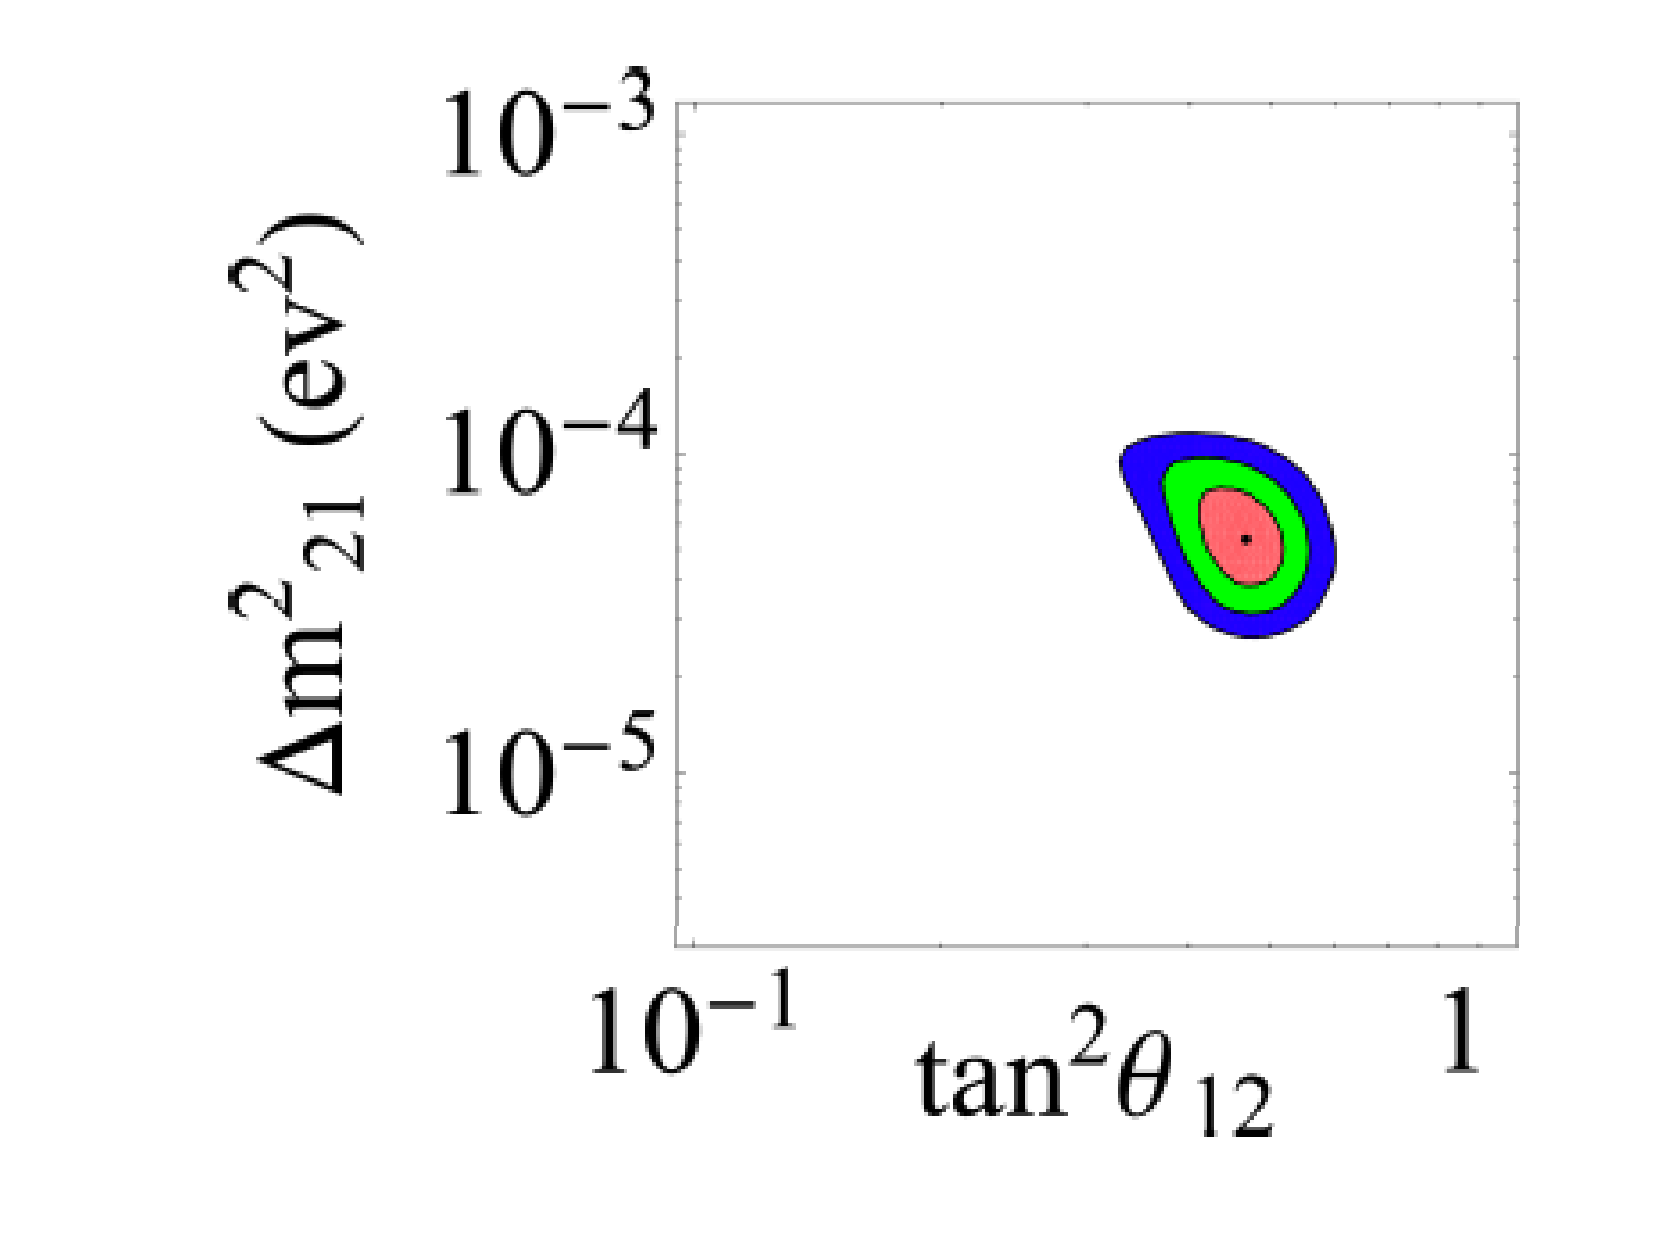
\includegraphics[width=0.6\textwidth]{chapters/neutrinophysics_images/theta_12}
\caption[Allowed region for $\theta_{12}$ and $\Delta m^2_{21}$]{\label{fig:theta_12_confidence}The current knowledge of the values of $\theta_{12}$ and $\Delta m^2_{21}$ represented as a plot of $\Delta m^2_{21}$ against $\tan^2\theta_{12}$. The contours give the $68.27\%$, $95.45\%$ and $99.74\%$ confidence level allowed regions for a global solar neutrino analysis. Figure adapted from \citep{Bellini2012}.}
\end{figure}

\subsection{Atmospheric Neutrinos and $\theta_{23}$}
Measurements of $\theta_{23}$ and the mass splitting $\Delta m^2_{31}$ were obtained from experiments measuring atmospheric neutrino oscillations from Super-Kamiokande\citep{SuperK2006}, combined with results from the K2K\citep{K2K2006} and MINOS\citep{MINOS2008} long-baseline accelerator neutrino experiments. Figure \ref{fig:theta_23_confidence} represents the allowed regions based on each experiment's results, along with the MINOS best fit value. The best-fit values are\citep{Mezzetto2010}:
\begin{equation}\label{eqn:atmospheric_parameters}
\sin^2 \theta_{23} = 0.50^{+0.07}_{-0.06}, ~~~~\left|\Delta m^2_{32} \right| \approx \left| \Delta m^2_{31} \right| = 2.40^{+0.12}_{-0.11} \times 10^{-3} \eV^2
\end{equation}

\begin{figure}
\centering
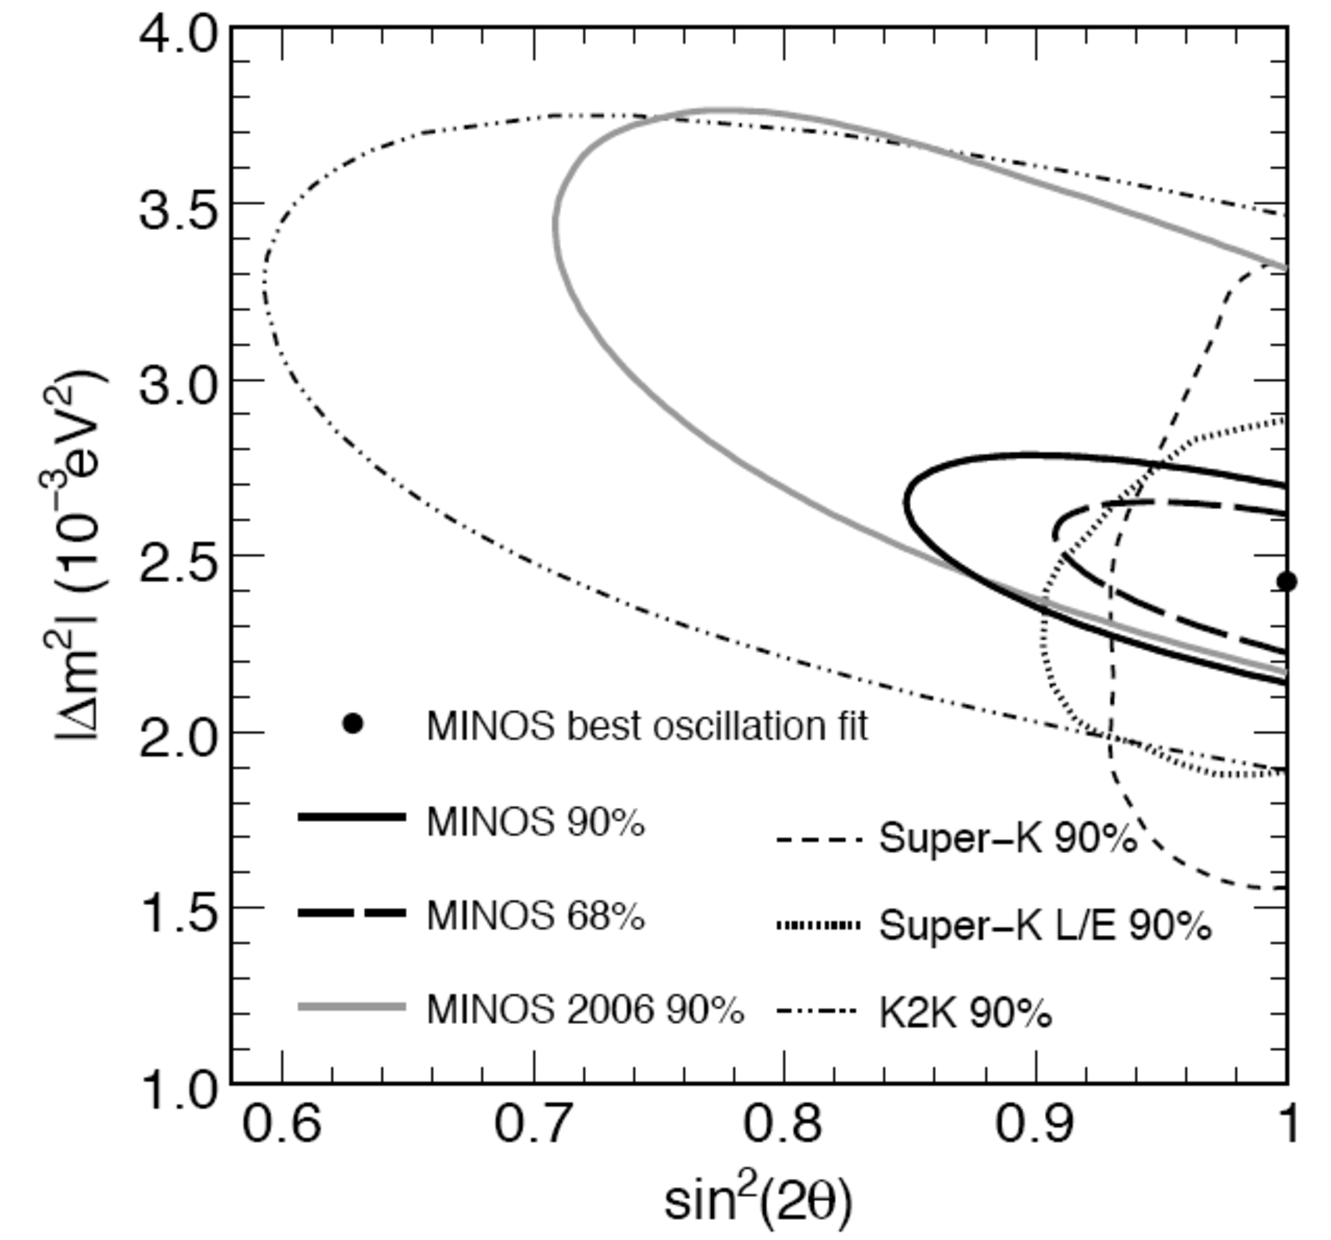
\includegraphics[width=0.6\textwidth]{chapters/neutrinophysics_images/theta_23}
\caption[Allowed region for $\theta_{23}$ and $\Delta m^2_{31}$]{\label{fig:theta_23_confidence}The current knowledge of the values of $\theta_{23}$ and $\Delta m^2_{31}$ as measured by the MINOS, Super-Kamiokande and K2K experiments, with allowed regions at $68\%$ and $90\%$ confidence levels. Figure taken from \citep{PDG2011}.}
\end{figure}

\subsection{Reactor Neutrinos and $\theta_{13}$}
From the PMNS matrix, equation \eqref{eqn:pmns_matrix_combined}, it is clear that the CP violating phase $\delta$ is always associated with a $\sin\theta_{13}$ term. This means that CP violation in the lepton sector requires a non-zero $\theta_{13}$. The T2K\citep{Abe2011} experiment published indications that $\theta_{13}$ was non-zero in 2011, but the measurement was claimed in 2012 by the Daya Bay reactor neutrino experiment. The Daya Bay collaboration published a result for non-zero $\theta_{13}$ with $5.2\sigma$ significance\citep{An2012}, quoting a measured value of:
\begin{equation}\label{eqn:reactor_parameters_dyb}
\sin^2 2\theta_{13} = 0.092 \pm 0.016 (\mathrm{stat}) \pm 0.005 (\mathrm{sys})
\end{equation}

Within a month of the Daya Bay result, the RENO reactor neutrino experiment also published a measurement of $\sin^2 2\theta_{13}$\citep{Ahn2012}:
\begin{equation}\label{eqn:reactor_parameters_reno}
\sin^2 2\theta_{13} = 0.103 \pm 0.013 (\mathrm{stat}) \pm 0.011 (\mathrm{sys})
\end{equation}

Since both the Daya Bay and RENO results are from rate-only analyses, i.e. looking for a deficit of $\bar{\nu}_e$ in the far detector, compared to the flux predicted based on measurements in the near detectors, and in the absence of oscillations, it is reasonably straightforward to combine the two results. The combination process involves averaging the values, weighted by their combined errors (weight $w = 1/\sigma^2$). In order for this to work, the errors should ideally be Gaussian distributed, and uncorrelated. While this is true for the statistical errors, it cannot be trivially assumed for the systematics, which may exhibit some correlation between the two experiments.

Ideally, such a combination would take the predicted and measured fluxes in each reactor--detector pair (across both experiments), and use a $\chi^2$ minimisation, weighted by the statistical and systematic uncertainties presented for each detector. In the absence of this detailed information, the best one can do is to assume Gaussian, uncorrelated errors, and proceed accordingly. This assumption is somewhat backed up by the parabolic shape of the $\chi^2$ versus $\sin^2 2\theta_{13}$ curves presented by the experiments\citep{An2012, Ahn2012}.

It turns out that the combined statistical and systematic errors for the two experiments are the same:
\begin{align}
\sigma_{\mathrm{Daya~Bay}} & = \sqrt{0.016^2 + 0.005^2} = 0.017 \\
\sigma_{\mathrm{RENO}} & = \sqrt{0.013^2 + 0.011^2} = 0.017 \nonumber
\end{align}
This simplifies the weighted average to a simple mean:
\begin{equation}
\left<\sin^2 2\theta_{13}\right> = \frac{0.092 + 0.103}{2} = 0.098
\end{equation}
The error on this combined quantity is $\sigma = \sqrt{1 / \sum w}$, which reduces to:
\begin{equation}
\sigma_{\mathrm{Combined}} = \frac{\sigma}{\sqrt{2}} = 0.012
\end{equation}
The combined result is therefore:
\begin{equation}\label{eqn:theta_13_combined}
\left<\sin^2 2\theta_{13}\right> = 0.098 \pm 0.012
\end{equation}

A more thorough combination, bringing in the T2K and MINOS results on $\theta_{13}$, is beyond the scope of this thesis, though such an analysis would allow the production of a confidence region plot showing the parameter space for $\theta_{13}$ and the $\Charge\Parity$ violating phase $\delta$ (the reactor experiments are measuring $\bar{\nu}_e$ disappearance, which is not sensitive to $\delta$; a $\nu_e$ appearance measurement is required).

\begin{figure}
\centering
\rotatebox{-90}{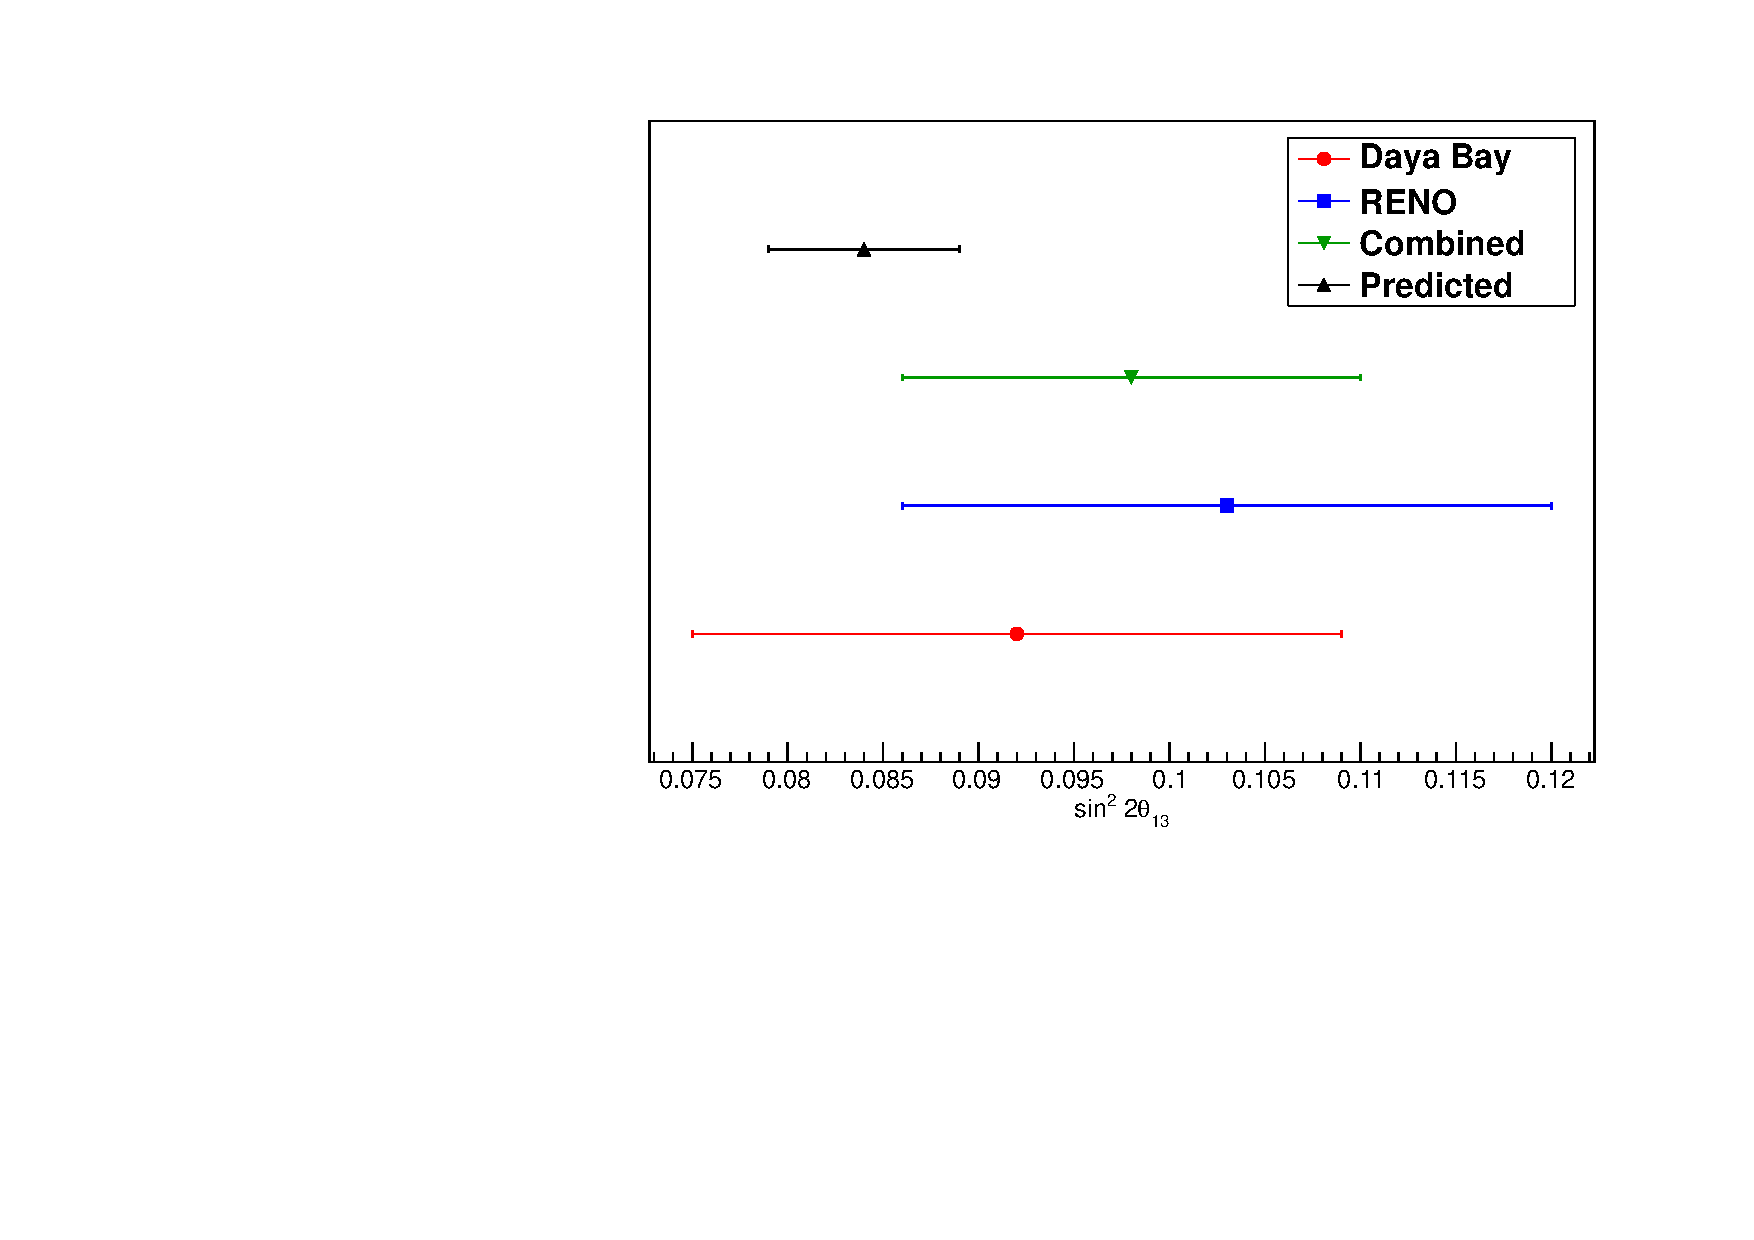
\includegraphics[width=0.6\textwidth]{chapters/neutrinophysics_images/theta_13_results}}
\caption[Comparison of measurements of $\sin^2 2\theta_{13}$]{\label{fig:theta-13_results}Comparison of measurements of $\sin^2 2\theta_{13}$ from the Daya Bay experiment (red), the RENO experiment (blue), a combination of the two results (green) and prediction by Harrison and Scott (black).}
\end{figure}

It is worth noting that in 2004, a prediction compatible with this value of $\sin^2 2\theta_{13}$ was made by Harrison and Scott, by relating $\sin\theta_{13}$ to the two mass-squared differences, $\Delta m^2_{21}$ and $\Delta m^2_{31}$\citep{Harrison2004}. Their prediction, motivated by the results available at the time, states:
\begin{equation}\label{eqn:theta_13_prediction}
\sin \theta_{13} = \sqrt{\frac{2\Delta m^2_{21}}{3\Delta m^2_{31}}}
\end{equation}

Converting this to a statement about $\sin^2 2\theta_{13}$, and neglecting terms with $\Delta m^4$ (or, equivalently, $\sin^4 \theta$) yields:
\begin{equation}\label{eqn:sin2_2theta_13_prediction}
\sin^2 2\theta_{13} = \frac{8 \Delta m^2_{21}}{3 \Delta m^2_{31}}
\end{equation}
Substituting in the global best-fit values for the two mass splittings, and propagating through the errors, one obtains:
\begin{equation}\label{eqn:prediction_sin2_2theta_13}
\sin^2 2\theta_{13,\,\mathrm{predicted}} = 0.084 \pm 0.005
\end{equation}

The two experimental results, along with the combined result and the predicted value, are shown in fig. \ref{fig:theta-13_results}.

\section{Open Questions in Neutrino Physics}
With a non-zero $\theta_{13}$ firmly established, the experimental focus will now shift to the determination of the $\Charge\Parity$ violating phase $\delta$. $\Charge\Parity$ violation in the lepton sector manifests as a difference between the vacuum oscillation probabilities for neutrinos and for antineutrinos, and could form part of an attractive mechanism for generating the observed baryon asymmetry of the universe through processes such as leptogenesis\citep{Riotto1999}.

Since the sign of the mass splitting $\Delta m^2_{31}$ is not known, there remains a question of \emph{hierarchy}; that is, whether there are two light neutrino mass states and one heavier (the so-called \emph{normal} hierarchy), or two heavy and one light (the \emph{inverted} hierarchy). 

The possible Majorana nature of neutrinos is currently being probed by neutrinoless double-$\beta$ decay experiments, including SuperNEMO\citep{SuperNEMO} and part of the physics programme for the SNO+ upgrade\citep{SNO+} to the SNO project.


\chapter{Detector Physics}\label{chapter:DetectorPhysics}
\section{Particle Detectors}
Particle detectors for high-energy physics experiments typically include a number of components, each designed to perform one specific task. A common design, based on a central interaction region (i.e. in collider experiments) uses a fine-grained tracker close to the interaction region, with calorimeters and coarse trackers further out. Muon chambers around the outside provide a signal if a particle penetrates the calorimeters and leaves the detector entirely. In this scenario, detector elements are designed to perform either tracking or calorimetry. A tracker provides details of the passage of ionising particles through a detector, usually in the form of spatial points or \emph{hits}. Hits are combined using a track reconstruction algorithm, yielding parameters which estimate the path a particle took (usually a straight line, or a curve or helix in a magnetic field). Tracks may be back-projected to estimate the interaction vertex, and curvature in a magnetic field provides a measurement of particle momentum~\citep{Green2008}. 

The history of tracking detectors began with the bubble chamber, in which each event consists of images of the bubbles produced when ionising particles pass through a detector, recorded onto photographic plates. The signal readout was performed by manually scanning each photographic plate. Wire chambers and drift chambers also provide this tracking capability, and they are preferred since the readout is electronic, and can be automated. In a drift chamber, ionising particles release electrons from the gas that fills the chamber. These electrons drift in an electric field (provided by field wires) towards a signal wire where the charge is read out. The position resolution of such a detector depends on the wire pitch. The current generation of particle physics experiments also makes use of Silicon trackers, which use the properties of Silicon semiconductors to trap ionisation charge into pixels which can be read out electronically. These can provide extremely high resolution (on the order of $\micron$) but are also rather expensive.

Calorimeters deal with the determination of the kinetic energy of a particle (or of an electromagnetic or hadronic shower produced by an initial particle). The energy losses are measured by a detector medium which produces light or charge signals proportional to the energy deposited. With a sufficiently large calorimeter, particles of interest will come to a stop completely within the calorimeter, and the total kinetic energy can be measured. Liquid Argon is currently used in the calorimeters of a number of experiments, including the electromagnetic calorimeter of the ATLAS~\citep{ATLAS1999} experiment. Liquid Argon is usually used to build sampling calorimeters, in which layers containing liquid Argon are alternated with layers of a high-density absorber such as Lead. This technology provides calorimetry in conjunction with high stopping power. The scintillation light from the liquid Argon is generally wavelength shifted in order that the peak wavelength coincides with the peak photon detection efficiency of a photosensitive device. Liquid Argon calorimetry is therefore a demonstrated and proven technology~\citep{Aprile2006}.

\section{Physics Motivation}
Many of the fundamental results of experimental neutrino physics have been provided by large underground neutrino detectors such as SNO and Super-Kamiokande. These couple a large target mass with the shielding that several hundred metres of rock provides against many sources of background events (cosmic rays, for instance). The next generation of experiments will require an order of magnitude increase in detector size to reach new physics goals.

A large, high-mass detector on the order of $100\kton$ to $1\Mton$ would provide sensitivity for a number of new scientific opportunities, including a precision measurement of the neutrino mixing angle $\theta_{13}$ as well as sensitivity to the $\Charge\Parity$ violating phase $\delta$ (and hence to leptonic $\Charge\Parity$ violation measurements). In addition to this conventional neutrino physics programme, such a detector would be able to study neutrinos from supernovae, permitting studies of the mechanisms of the explosions, as well as having a sensitivity to proton decay with lifetimes of up to $10^{35}$ years, a number of significance to several theoretical models~\citep{Laguna2009}.

\section{Liquid Argon Time Projection Chambers}
Ionising radiation moving through \ac{LAr} generates both ionisation charge and scintillation light signals, though the energy resolution of the scintillation light is typically poor compared to that of the ionisation charge, since only a small number of the emitted photons can usually be detected~\citep{Aprile2006}. \aclp{LAr TPC} were first proposed by Carlo Rubbia in 1977~\citep{Rubbia1977}, when he noted that \ac{LAr} has several useful properties as a detector medium, including high density, long electron drift times, and relatively high abundance making it cheap to obtain in large quantities.

The ionisation charge produced by a primary ionising particle can be drifted through an applied electric field to a readout plane (anode), see fig. \ref{fig:tpc-schematic}.

\begin{figure}
\centering
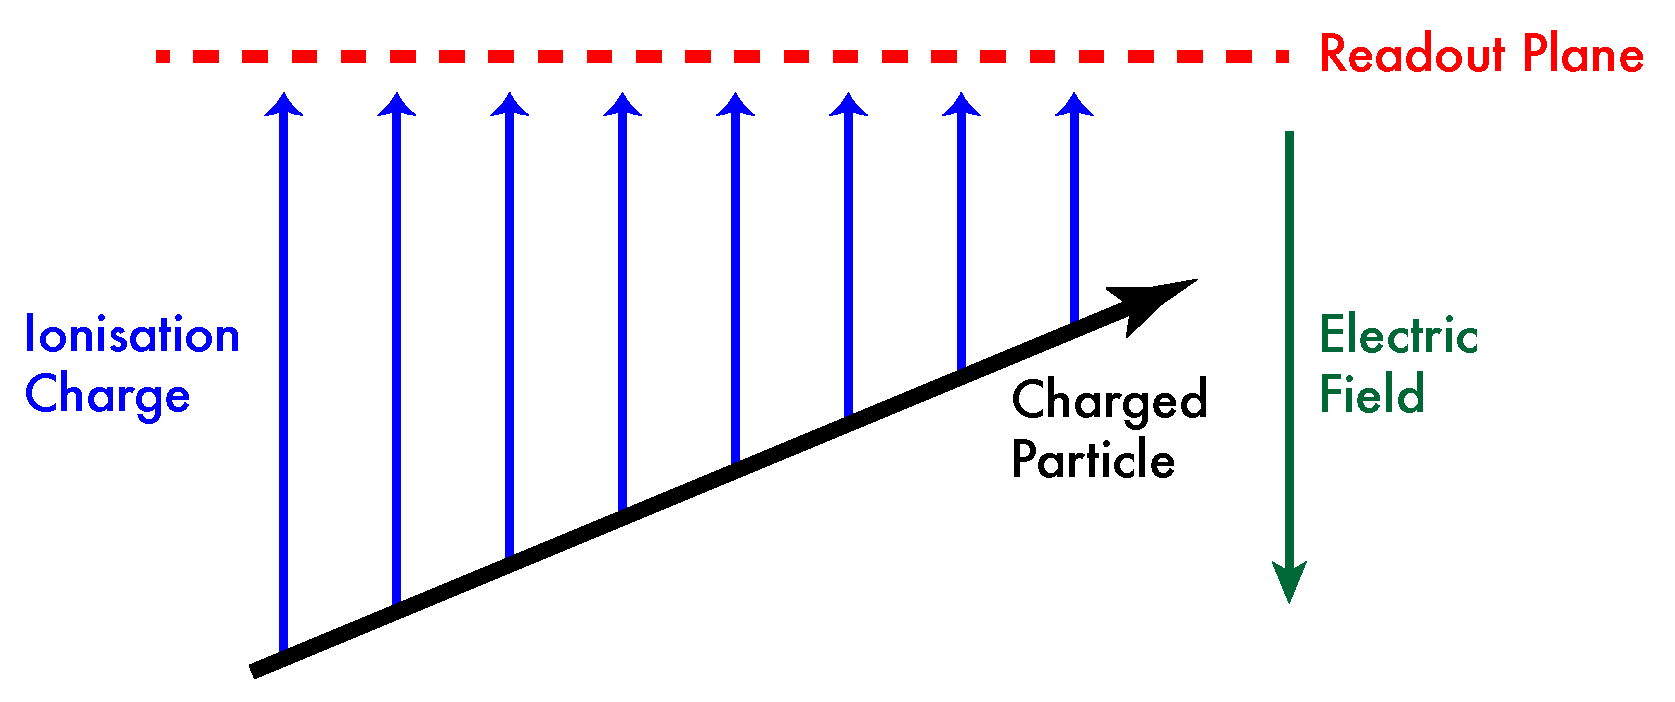
\includegraphics[width=\textwidth]{chapters/detectorphysics_images/TPC-Schematic}
\caption[Schematic diagram of the operation of a time-projection chamber]{\label{fig:tpc-schematic}Schematic diagram of the operation of a time-projection chamber. An incident ionising particle produces ionisation charge, which drifts in an applied electric field to a readout plane. The readout plane provides a two-dimensional $(x,y)$ position measurement, and the depth $z$ can be determined from the drift time $t$ taken for charge to arrive at the readout plane.}
\end{figure}

\subsection{Production of Ionisation Charge}\label{sec:production-ionisation-charge}
The amount of ionisation charge $Q$ that drifts to a readout plane is smaller than that initially produced by the passage of an ionising particle $Q_0$, since some of the electron-ion pairs undergo recombination processes, i.e. $Q = \mathcal{R}Q_0$ with some \emph{quenching factor} $\mathcal{R}$. The recombination is described empirically by Birk's Law~\citep{Birks1964}:
\begin{equation}\label{eqn:birks_law}
    Q = \frac{Q_0}{1 + k_E / \epsilon}
\end{equation}
where $k_E$ is a recombination constant, to be fitted to data, and $\epsilon$ is the applied electric field strength. In terms of the stopping power $dE/dx$, this is written:
\begin{equation}\label{eqn:birks_law_dEdx}
    Q = \frac{Q_0}{1 + k_Q\, dE/dx}
\end{equation}
with $k_Q(\epsilon) = k_E / \epsilon$.

The {\sc Icarus} experiment~\citep{Amoruso2004} measured the quenching factor $\mathcal{R}$ as a function of the applied field and $dE/dx$, finding $\mathcal{R} = 0.71$ for $dE/dx$ from minimum ionising particles up to $\sim 30 \MeV \gram^{-1} \cm^2$ in an applied field of $0.5 \kvolt \cm^{-1}$. They found, however, that their data was best described with an additional normalisation constant $A$:
\begin{equation}\label{eqn:icarus_quenching}
Q = A\frac{Q_0}{1 + k_E/\epsilon \, dE/dx}
\end{equation}
with $A=0.800\pm0.003$ and $k_E = 0.0486\pm 0.0006 \kvolt \cm^{-1}$. This updated quenching factor has been applied in the Warwick \emph{Lamu} simulation package for liquid Argon detectors (see section \ref{sec:lamu} for further details).

\subsection{Drifting Charge}
Charge transport through a medium such as \ac{LAr} is governed by the mobility $\mu$ of charge carriers (electrons)~\citep{Aprile2006}. The drift velocity $\vec{v}$ is:
\begin{equation}\label{eqn:charge_transport}
    \vec{v} = \mu \vec{E}
\end{equation}
where $\mu$ is constant for low electric fields $\vec{E}$. An electron is considered to be \emph{quasifree} when the mobility in the absence of an electric field, $\mu_0$, is greater than $10 \cm^2 \volt^{-1} \second^{-1}$. For \ac{LAr}, where $\mu_0 = 625 \pm 15 \cm^2 \volt^{-1} \second^{-1}$~\citep{Aprile2006}, the drift velocity is large and drift lengths are limited primarily by impurities in the Argon, which capture the charge.

Another constraint on the drift length is the reduction in spatial resolution due to \emph{transverse diffusion} of drifting charge. As the charge drifts from the point of creation to the readout plane, diffusion perpendicular to the direction of motion acts to spread out the electron cloud. For long drift lengths, this reduces the $xy$ resolution which can be achieved at the readout plane.

\subsection{Wire Readout}
In most current and planned \acsp{TPC} the readout plane consists of a grid of wires, attached to charge amplifiers and subsequent electronics to read the charge signal that collects on each wire. Coincidence of signals on $x$ and $y$ wires provides a two-dimensional view of charge arriving at the readout plane. The {\sc Icarus} T600~\citep{Amerio2004} detector, with a $500\ton$ fiducial mass, demonstrated the success of wire plane readout on a small scale. Projects including MODULAr~\citep{Baibussinov2008} plan to carry the concept to larger detectors by grouping many {\sc Icarus}-style modules together. Alternative plans by collaborations such as LANNDD~\citep{Cline2003} use a single \ac{LAr} volume, internally segmented by readout planes.

Whilst the wires are inexpensive, large wire plane detectors require many electronics (readout) channels, each of which carries significant cost. For a $100\kton$ detector, this cost is substantial, and can be reduced only by using longer wires (which requires higher tension in the wires themselves, and presents an engineering challenge) or by increasing the inter-wire spacing, thus reducing the spatial resolution of the detector. Another option would be to increase the drift length, but this also results in degraded spatial resolution due to transverse diffusion of charge as it drifts.

\subsection{Thick Gas Electron Multipliers}
A \ac{TGEM} is a \ac{PCB} of thickness on the order of $1\mm$, with copper cladding on both sides. Holes are drilled into the \ac{PCB} at regular intervals, with diameters on the order of $1\mm$ and spaced by $< 1\mm$. The holes may be further shaped by etching e.g. to smooth rough edges from the drilling process. An electric potential is applied across the two Copper electrodes, creating a strong field in the holes and extending into the region around them. Electrons arriving at the \ac{TGEM} are focused into the holes by this field. The high field strength ($> 1.5 \kvolt \mm^{-1}$) within the holes causes rapid acceleration of the electrons.

If the \ac{TGEM} is in gaseous Argon, the accelerated electrons cause ionisation of Argon in the hole, freeing more electrons in an avalanche process. In this way, the \ac{TGEM} acts as a charge multiplier. In liquid Argon, the mean free path of electrons is much shorter than in gas, and the electrons do not gain sufficient energy to ionise an Argon atom (the ionisation energy of Argon is $23.4\eV$~\citep{Aprile2006}). Some of the electrons do, however, gain enough energy to excite electrons in Argon atoms ($11.55\eV$ threshold~\citep{Stewart2010}), which subsequently emit photons and allow for optical readout of the \ac{TGEM}~\citep{Lightfoot2009}.

The light produced by excitation processes in the holes of a \ac{TGEM} immersed in liquid Argon could be imaged and a reconstruction procedure applied to obtain the $(x,y)$ position of the hole(s) in which light was produced. As an alternative to wire plane readout, this optical readout procedure could have a much lower cost, due primarily to a reduction in the number of readout channels required. One approach would be to image a large area (on the order of $1 \metre^2$) with a single \ac{CCD} camera. This scenario is complicated by the necessity to focus the light onto the \ac{CCD}, and the time resolution which could be achieved is limited by the frame rate of the \ac{CCD}. In order for the time resolution to match that of the $xy$ plane, a \ac{CCD} that operates at frequencies of $\sim 1\MHz$ (and with high efficiency in the cold environment of \ac{LAr}) would be required. Such devices do not yet exist.

The second option is to use a sparse array of Silicon photomultipliers. These devices have high quantum efficiency and provide single photon sensitivity. Using a grid of silicon photomultipliers, it is possible to determine the position of a light source based on the relative intensities recorded at several detectors (see section \ref{sec:point-source-recon}).

\section{Point Light Source Reconstruction}\label{sec:point-source-recon}
In order that the position resolution and associated measurement uncertainty associated with reconstructing point light sources on a plane could be estimated, I wrote a simulation that produces a \emph{flux map} for a detector plane some distance $\Delta z$ from a plane of point light sources. This detector flux map is then used to calculate the integrated light intensity seen by a photosensitive device with a given area, active area and quantum efficiency. Such device areas can be positioned on the detector plane, and the output from the simulation then provides a list of intensities at each detector from a given distribution of sources. A visualisation of this output is show in fig. \ref{fig:flux-example}.

\begin{figure}
\centering
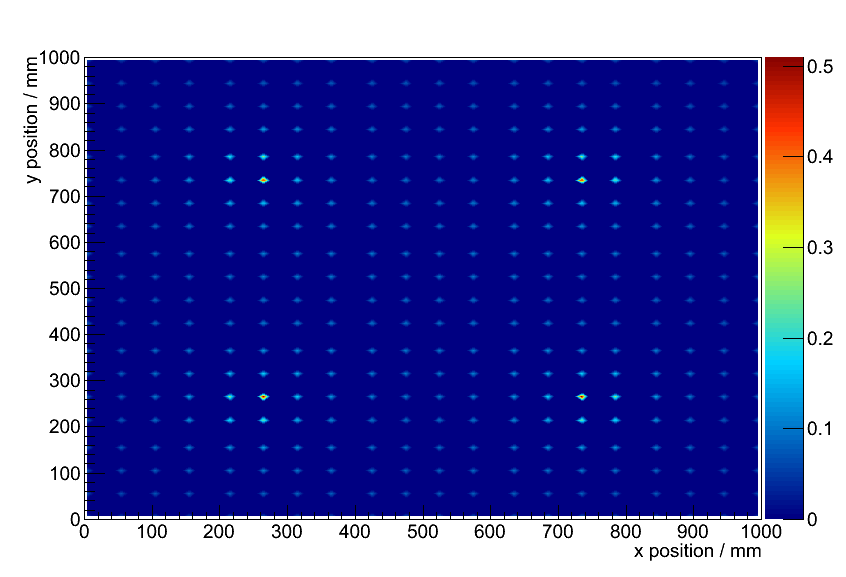
\includegraphics[width=0.85\textwidth]{chapters/detectorphysics_images/four-sources}
\caption[Simulation of light intensity recorded by a sparse array of photodetectors]{\label{fig:flux-example}Simulation of light intensity recorded by a sparse array of photodetectors from four light sources, normalised to the intensity of the sources. The sources are located at $(0.25, 0.25) \metre$, $(0.25, 0.75) \metre$, $(0.75, 0.25)\metre$ and $(0.75, 0.75) \metre$.} 
\end{figure}

This simulation was used by G. Rutter and M. Richards to develop an iterative algorithm for position reconstruction~\citep{Rutter2011}. The algorithm requires an initial estimate of the position of a source, which can be obtained from a global approach such as that used to reconstruct position in Anger cameras~\citep{Anger1958}. Once this seed position is established, the closest $2\times 2$ square of photosensors surrounding the source is chosen and the reconstructed position iteratively refined by assuming that light from the source propagates freely (i.e. spherically). The ratio of intensities seen by detectors $D_1$ and $D_2$ is given by~\citep{Rutter2011}:
\begin{equation}\label{eqn:ratio-detector-intensities}
\alpha = \frac{I_1}{I_2} = \frac{r_2^2}{r_1^2} = \frac{x_2^2 + y_2^2 + h^2}{x_1^2 + y_1^2 + h^2} 
\end{equation}
where the height $h$ is fixed and the coordinates are distances to the detectors $D_1$ and $D_2$. A similar ratio $\beta$ is constructed for detectors $D_1$ and $D_3$. The detector which is shared between the two ratios ($D_1$) is the one which recorded the highest light intensity. The radius $r$ is from source to detector.

Since the inter-detector spacing is fixed, the value of $x_1$ fixes the value of $x_2$, and similarly for the $y$ values. By fixing $x$ values, the $y$ values can be recomputed using equation \eqref{eqn:ratio-detector-intensities}, providing an improved estimate of the $y$ position of the source. This process can be repeated with the $y$ values fixed to improve the $x$ estimate, iteratively converging on the true source position until the difference in coordinates between iterations becomes small compared with other experimental uncertainties (or to a predefined tolerance), see fig. \ref{fig:iterative-source-recon}. The total uncertainty resulting from this procedure is shown as a function of the distance between source and detector planes in fig. \ref{fig:detector-spacing}, where the detectors are arranged in a square grid over a $1\metre^2$ area, with the quoted number of detectors per row, and the reconstruction is of a single point light source. This provides an optimisation procedure for determining the detector coverage required to obtain the desired uncertainty on position resolution.

The spatial resolution is limited by statistical uncertainty, which gives rise to the curved shape seen in fig. \ref{fig:detector-spacing}. A small distance between the source and detector planes yields small effective photodetector areas, reduction in the number of photons received from the source, and a corresponding deterioration in resolution. A large distance results in reduced photon flux over the active area of the photodetector, and again reduces the spatial resolution. These effects generate the curves displayed in the figure, which can be viewed as an optimisation of the spacing between the source and detector planes, for a given array geometry.

The advantage of using this iterative procedure over simply fitting the intensity measurements as for an Anger camera is that the iteration can continue until the uncertainty on the position of the light source falls below some threshold. Fitting provides a source position with some associated uncertainty, but the iterative procedure can be used to reduce this uncertainty to a chosen acceptable level, matching the desired position resolution of the detector. If the photodetector grid layout does not physically provide sufficient resolution, continued iteration of the algorithm will eventually provide no improvement to the knowledge of the position of the light source, and this is the basis for the optimisation described above.

\begin{figure}
\centering
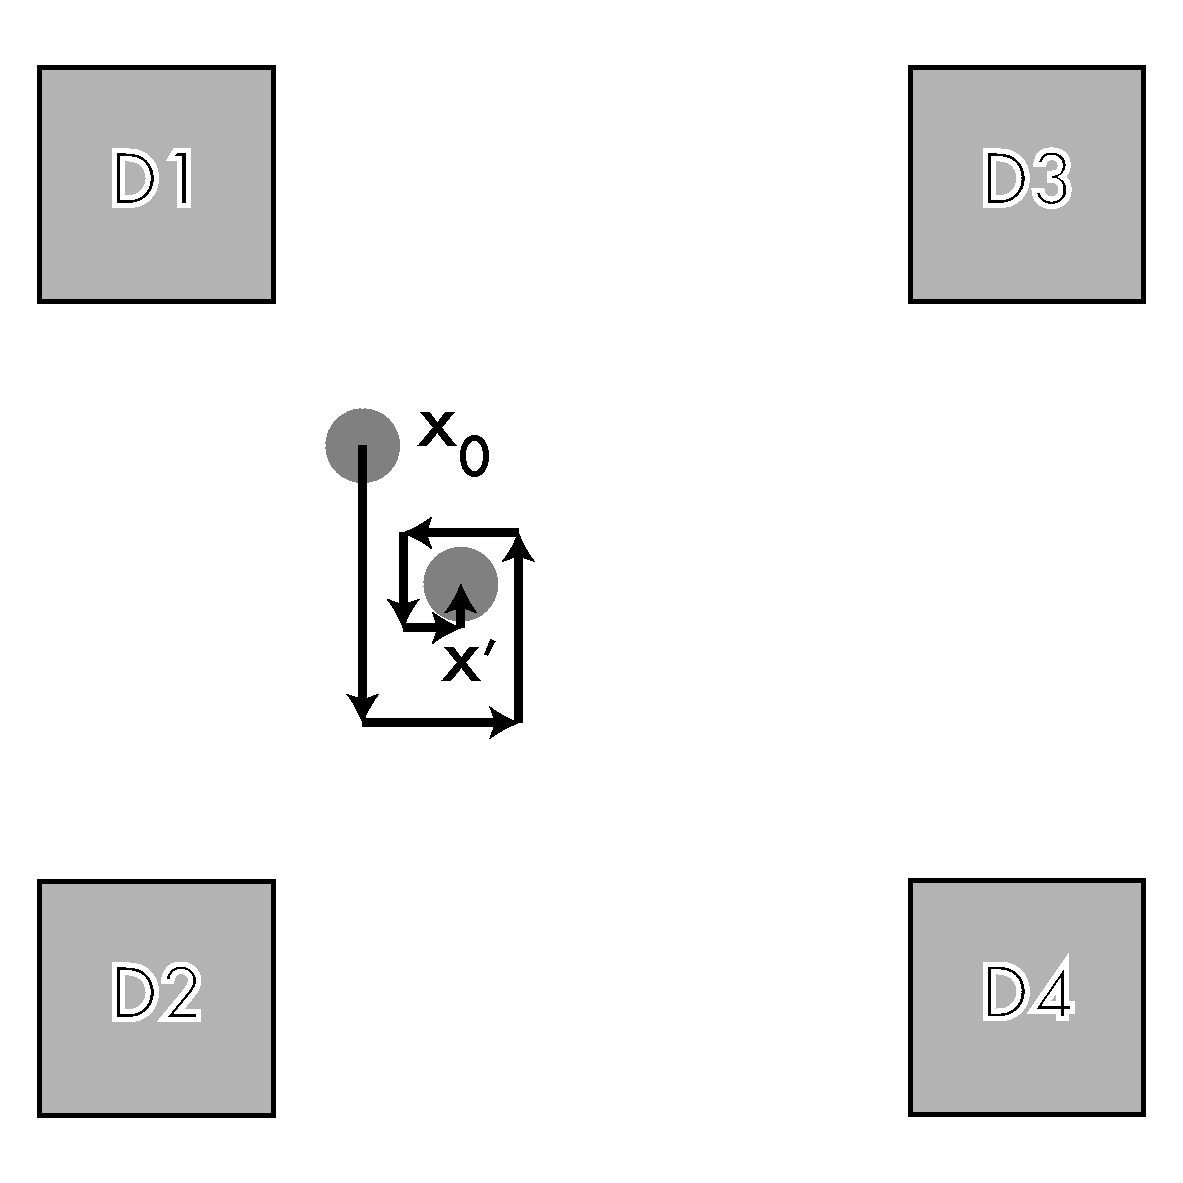
\includegraphics[width=0.5\textwidth]{chapters/detectorphysics_images/Iterative-Source-Recon}
\caption[Iterative point light source position reconstruction]{\label{fig:iterative-source-recon}Iterative reconstruction of the position of a point light source using the ratio of light intensities captured by the surrounding photodetectors. Each step updates either the $x$ or $y$ coordinate by constraining the $y$ or $x$ coordinate and using the known spacing between detectors.}
\end{figure}

\begin{figure}
\centering
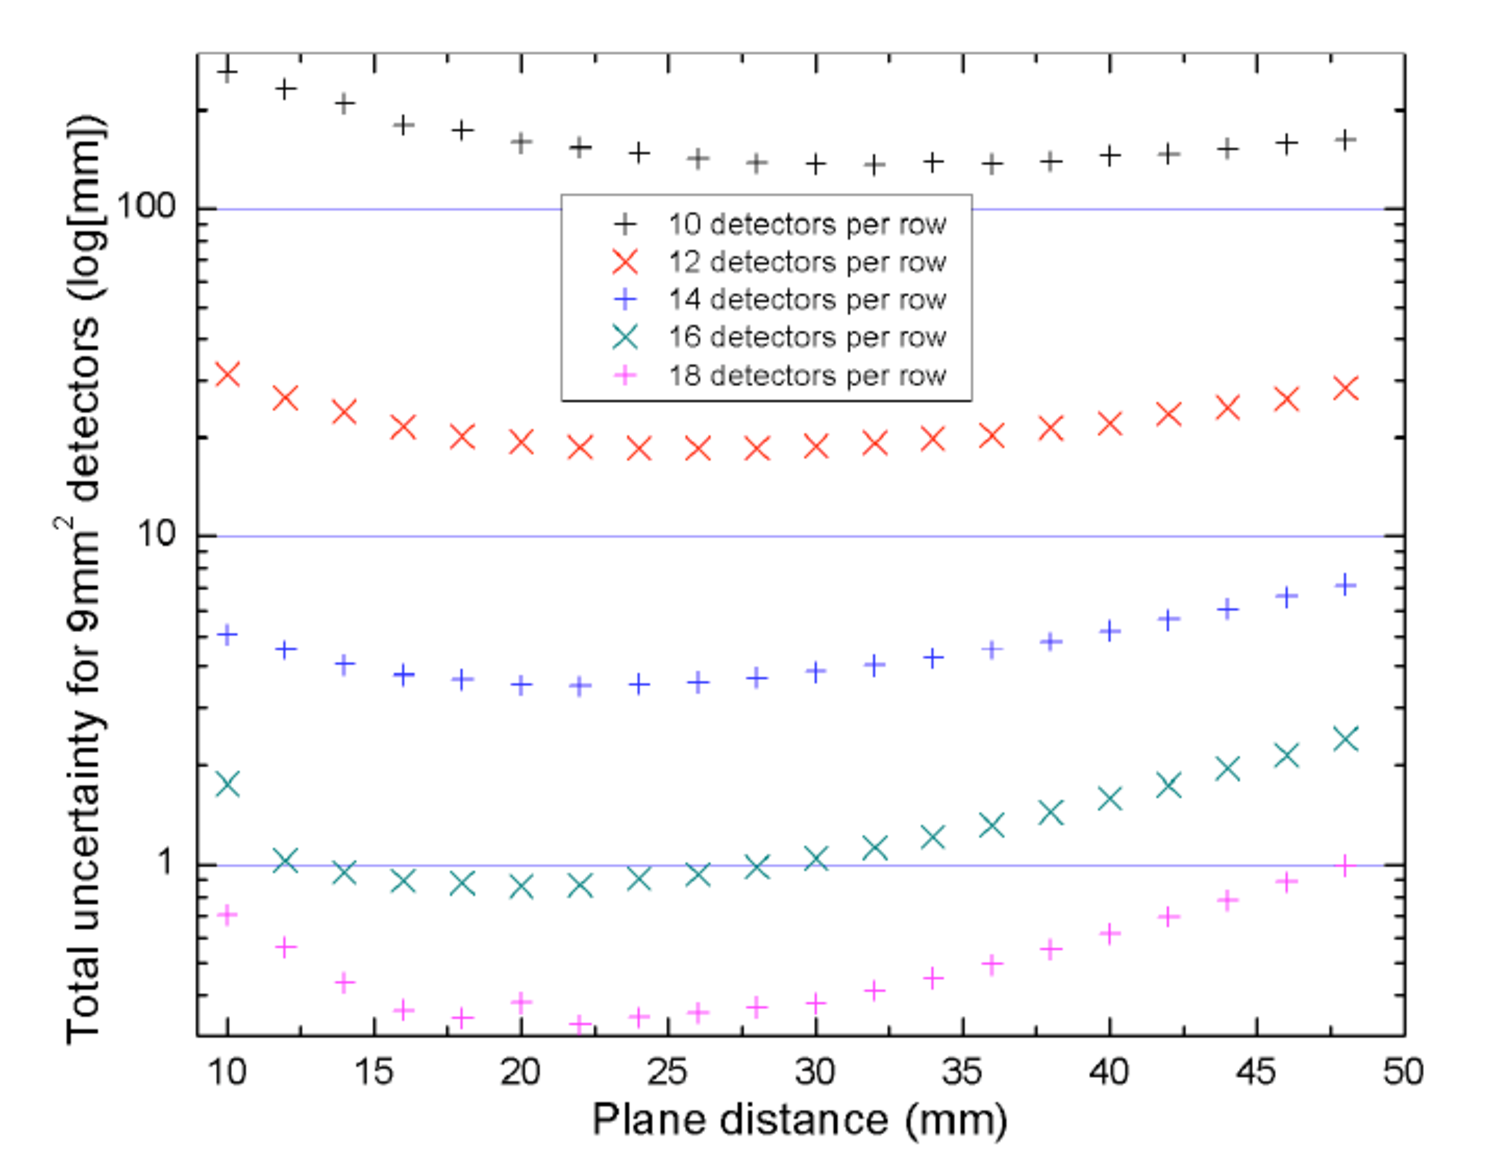
\includegraphics[width=0.6\textwidth]{chapters/detectorphysics_images/detector-spacing}
\caption[Uncertainty on position resolution for several sparse array detector densities]{\label{fig:detector-spacing}The uncertainty on the reconstructed position of a point light source resulting from the iterative procedure discussed in the text, as a function of source--detector plane spacing, for five different sparse array densities (detector--detector spacings). Figure taken from \citep{Rutter2011}.}
\end{figure}

\section{The Lamu Simulation}\label{sec:lamu}
Lamu is a Geant4~\citep{Geant4} simulation for liquid Argon volumes which consist of cylinders of configurable radius and height. It includes full modelling of physics processes according to the {\sc qgsp\_bic\_hp}\footnote{{\sc qgsp\_bic\_hp} is a standard Geant4 physics list, which applies a string model for the interactions of high energy hadrons. In addition to the basic string model ({\sc qgsp}), the list uses binary cascade modelling ({\sc bic}) for primary protons and neutrons below $10\GeV$ and high-precision data ({\sc hp}) for low energy neutrons. See \url{http://geant4.cern.ch/support/proc_mod_catalog/physics_lists/referencePL.shtml} for details.} physics list, with all electromagnetic and hadronic processes enabled. The energy loss of particles is modelled taking into account the quenching described in chapter \ref{sec:production-ionisation-charge}, and the \ac{LAr} volume is divided into $(3\times 3\times 3) \mm^3$ cubic voxels.\footnote{The $3\mm$ voxel side length was chosen to match the wire pitch of existing \acs{LAr TPC} detectors, including the {\sc Icarus}~\citep{Amerio2004} detector.} Charged particles are tracked through these voxels to zero energy or until they leave the detector, and the energy deposited in each voxel leads to a mapping between voxel coordinates and the total energy deposited within that voxel. The output from the simulation is this mapping, without any attempt to model drifting charge, readout technologies or subsequent electronics, all of which are dependent on experiment-specific details. A \ac{LAr} specific quenching factor is used to scale the energy deposited in each voxel by the passage of a charged particle through it. This factor is described in section \ref{sec:production-ionisation-charge}. The result is a three-dimensional point cloud corresponding to the energy deposition in the detector volume by a particular event. Events are stored in {\sc Root}~\citep{Root} files for subsequent analysis.

\subsection{Characterisation \& Testing of the Lamu Simulation}
In order to characterise the Lamu simulation, a number of tests were performed using simulated single particles produced by the Geant4 General Particle Source (GPS) generator~\citep{GeantGPS}.

In the first test, muons of fixed kinetic energy were started at the centre of a cylindrical detector volume, with radius $R$ and height $H=2R$. The radius was initially set to $1\metre$ and 100 events were generated. The radially outermost hit in each event was found, and the number of events with such hits lying within $10\cm$ of the detector wall recorded. The radius was increased in $1\metre$ intervals until greater than 95\% of the events were fully contained, i.e. the outermost hit was more than $10\cm$ from the wall. This study was performed at energies from $100\MeV$ to $5000\MeV$ in $100\MeV$ intervals, and the results are shown in fig. \ref{fig:lamu-containment-radius}.

The purpose of this study was to determine the maximum range of a muon of a given energy in liquid Argon, enabling the remainder of the work in this thesis to be done in the context of a simulation with geometry chosen so as to fully contain a muon produced at the centre of the detector. For example, all $\nu_\mu$ charged current events with an initial neutrino energy of $4500\MeV$ were simulated in a detector of $25\metre$ radius, in order to ensure that the resulting muons were fully contained.

\begin{figure}
\centering
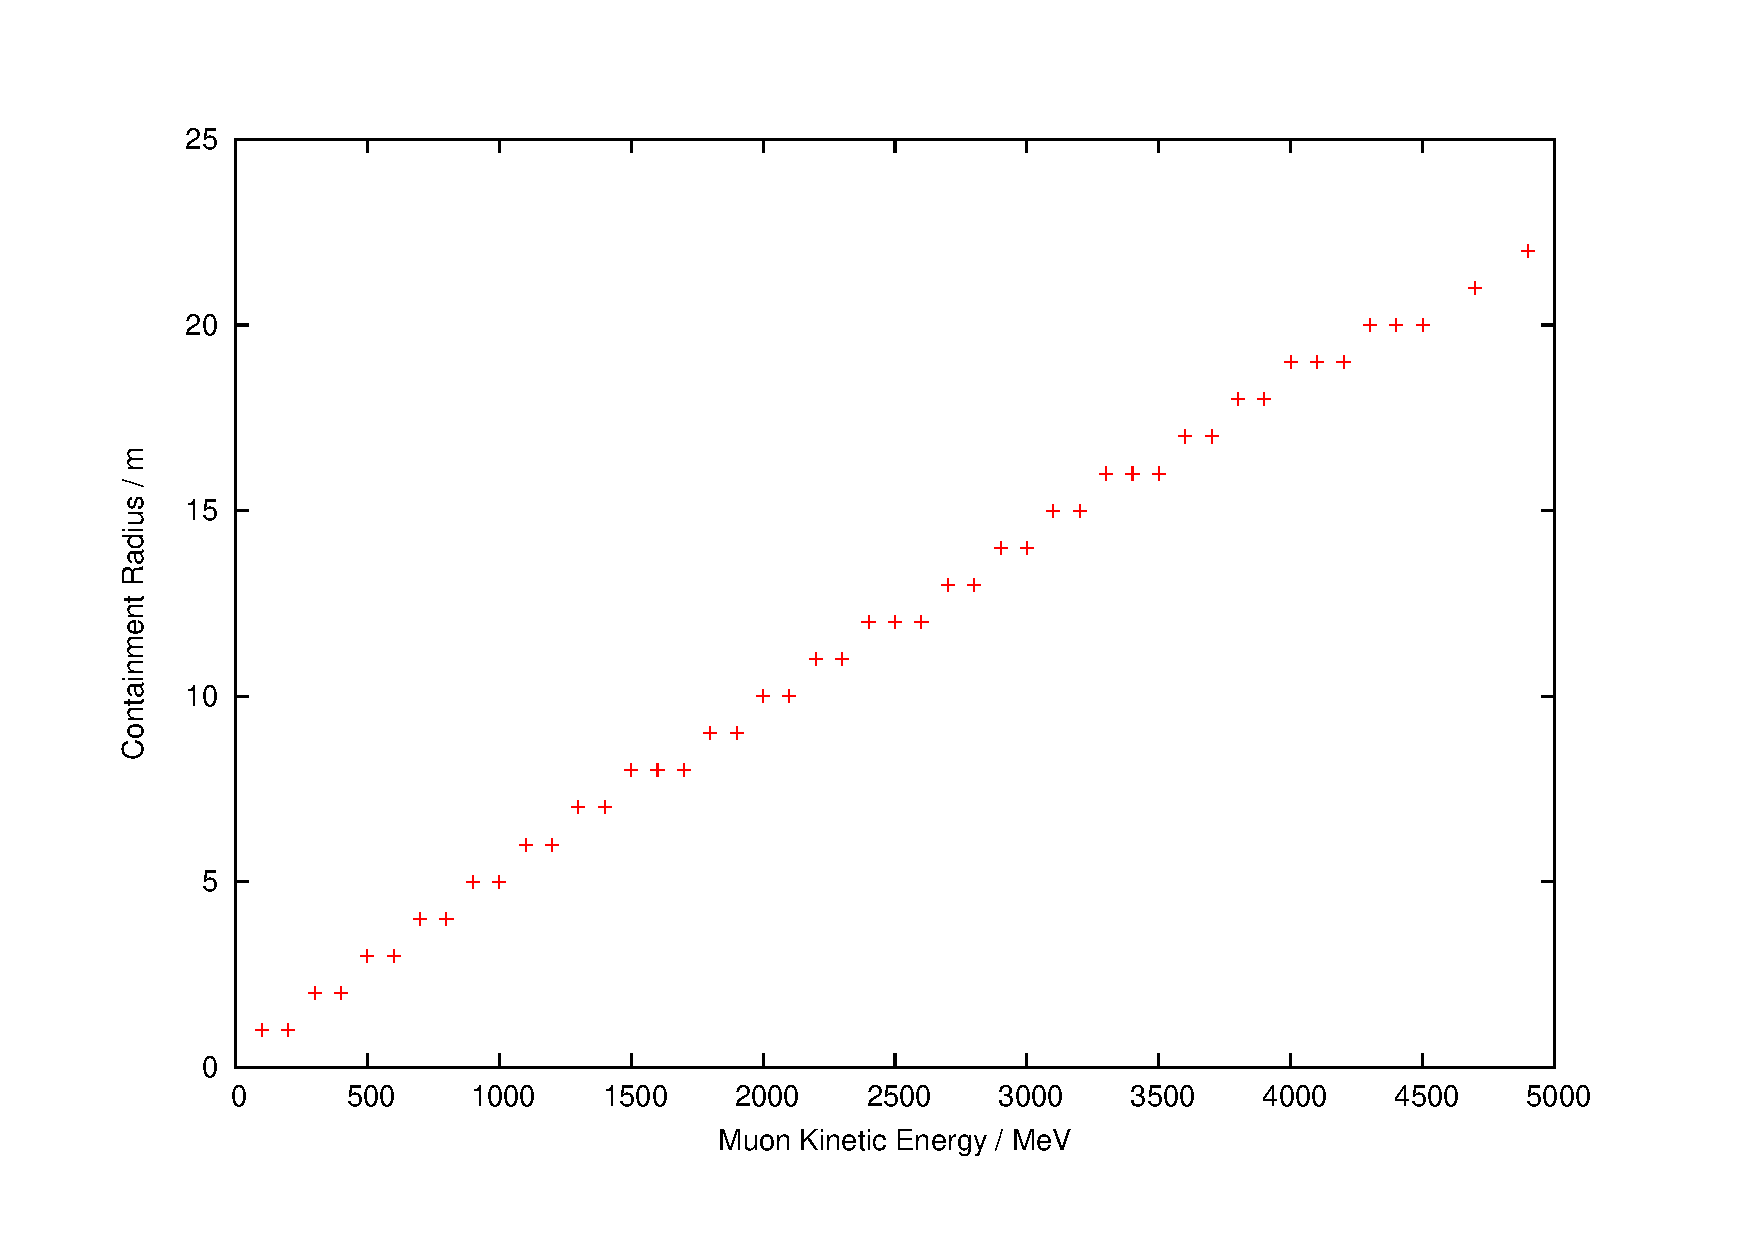
\includegraphics[angle=-90,width=0.9\textwidth]{chapters/detectorphysics_images/containment_radius}
\caption[Detector radius required for full containment as a function of energy]{\label{fig:lamu-containment-radius}Minimum detector radius required in order to fully contain muon tracks, as a function of the muon kinetic energy. This information is used to ensure that subsequent studies have fully contained primary particles.}
\end{figure}

The second test relates to the ionisation charge quenching factor built into the Lamu simulation. For this test, particles of several species were tracked through the detector with a fixed initial kinetic energy, and the total energy deposited was recorded by summing the energy deposited in each voxel. The results of this study are shown in fig. \ref{fig:detector_energy_ratios}, giving the ratio of energy deposited in the simulated \ac{LAr} volume to the initial kinetic energy of the particle. This is plotted separately for muons, protons, electrons, and charged pions.

For each plot, the calculation of energy deposited took into account only hits produced by a particle of the species under consideration. For muons, the ratio is fairly consistent with the quenching formula since a muon will behave much the same irrespective of energy (within the range considered). For protons and charged pions, the higher energy particles are more likely to undergo hadronic interactions resulting in particles of different species. In this way, the energy deposited by protons drops as the proton energy increases, since most of the energy is carried away by products of hadronic interactions. The same applies for pions.

In the case of electrons, as the energy increases, the chance of an electromagnetic shower occurring also increases in analogy to the hadronic showers of protons and charged pions. However, the ratio curve plotted in fig. \ref{fig:detector_energy_ratios_electron} does not show a significant drop since the (charged) products of an electromagnetic shower are themselves electrons, and all energy deposited by electrons was counted towards the deposition from the primary particle.

\begin{figure}
\centering
\subfigure[Muon]{
    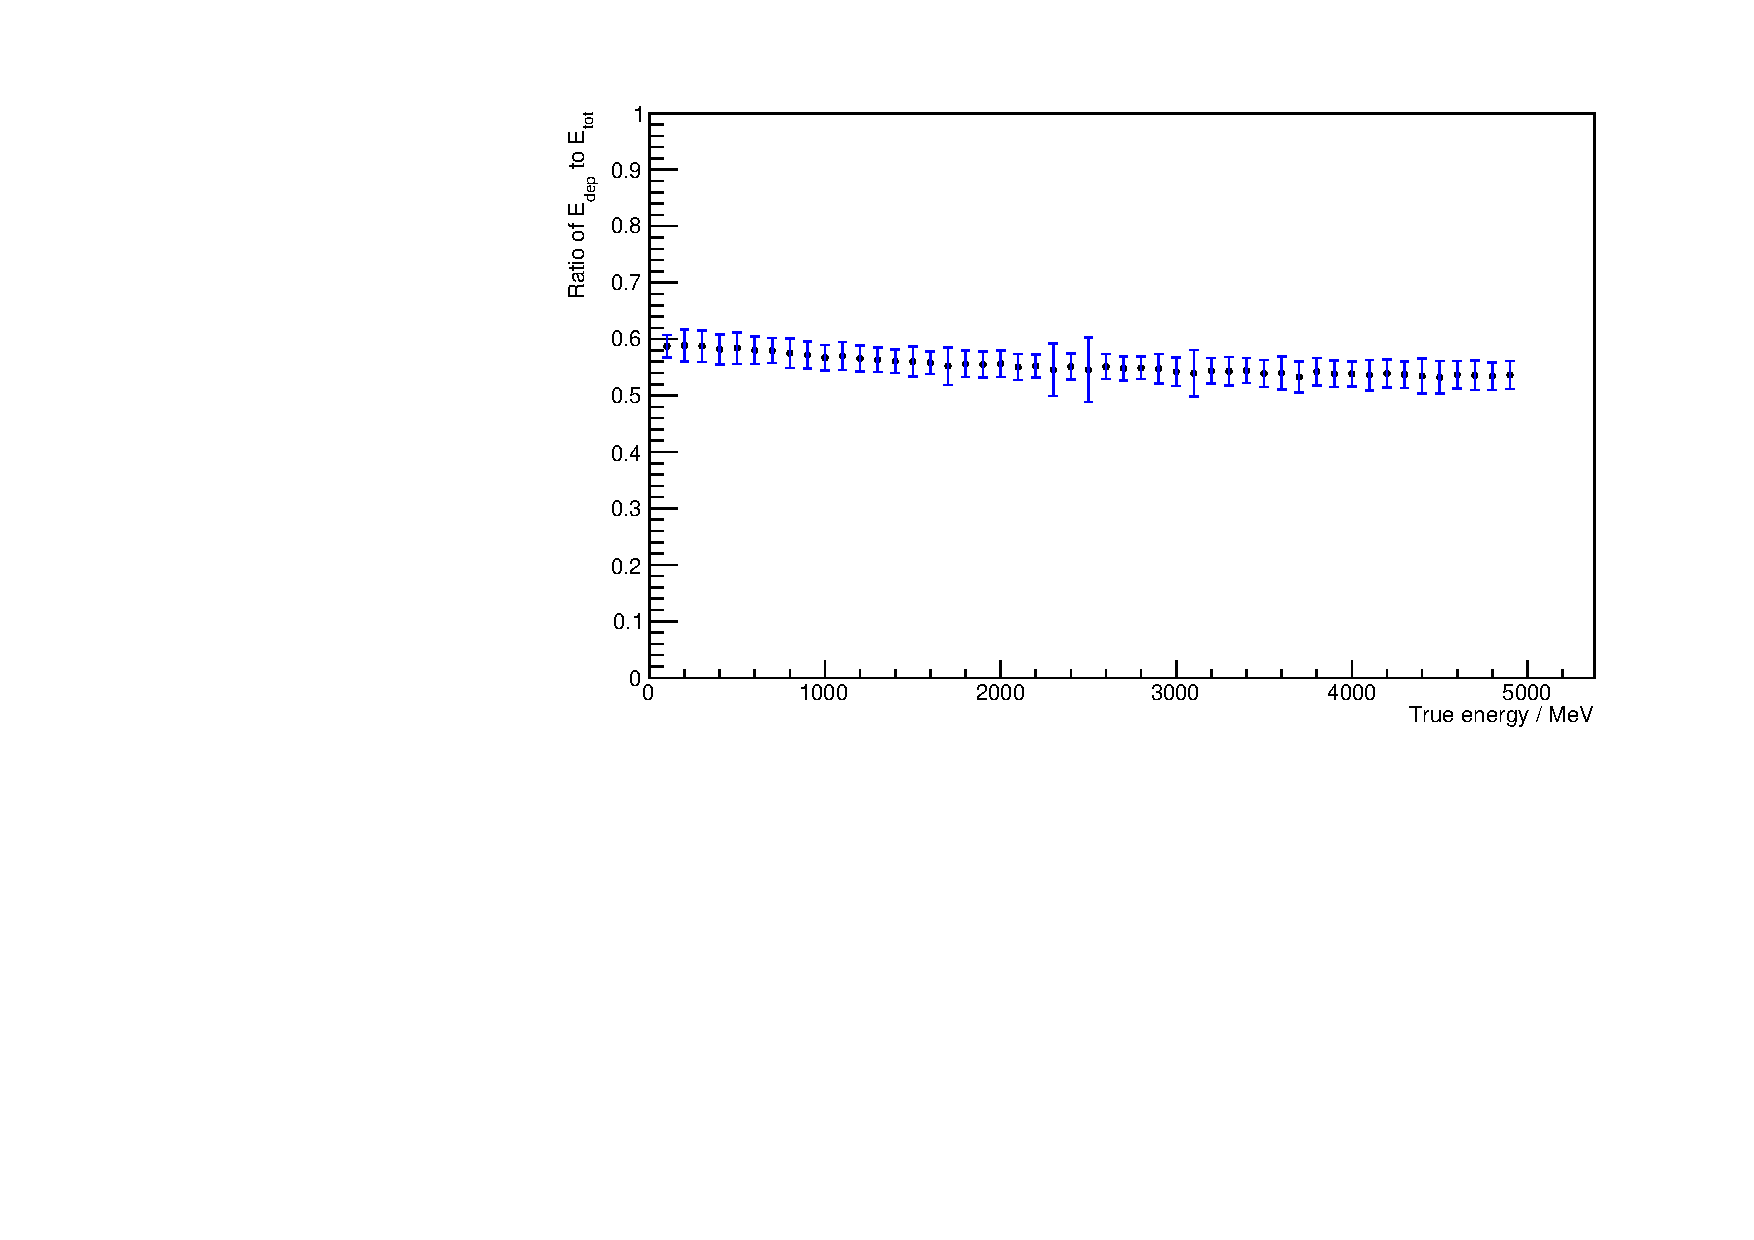
\includegraphics[angle=-90,width=0.45\textwidth]{chapters/detectorphysics_images/muon-energy-ratio}
    \label{fig:detector_energy_ratios_muon}
    }
\subfigure[Proton]{
    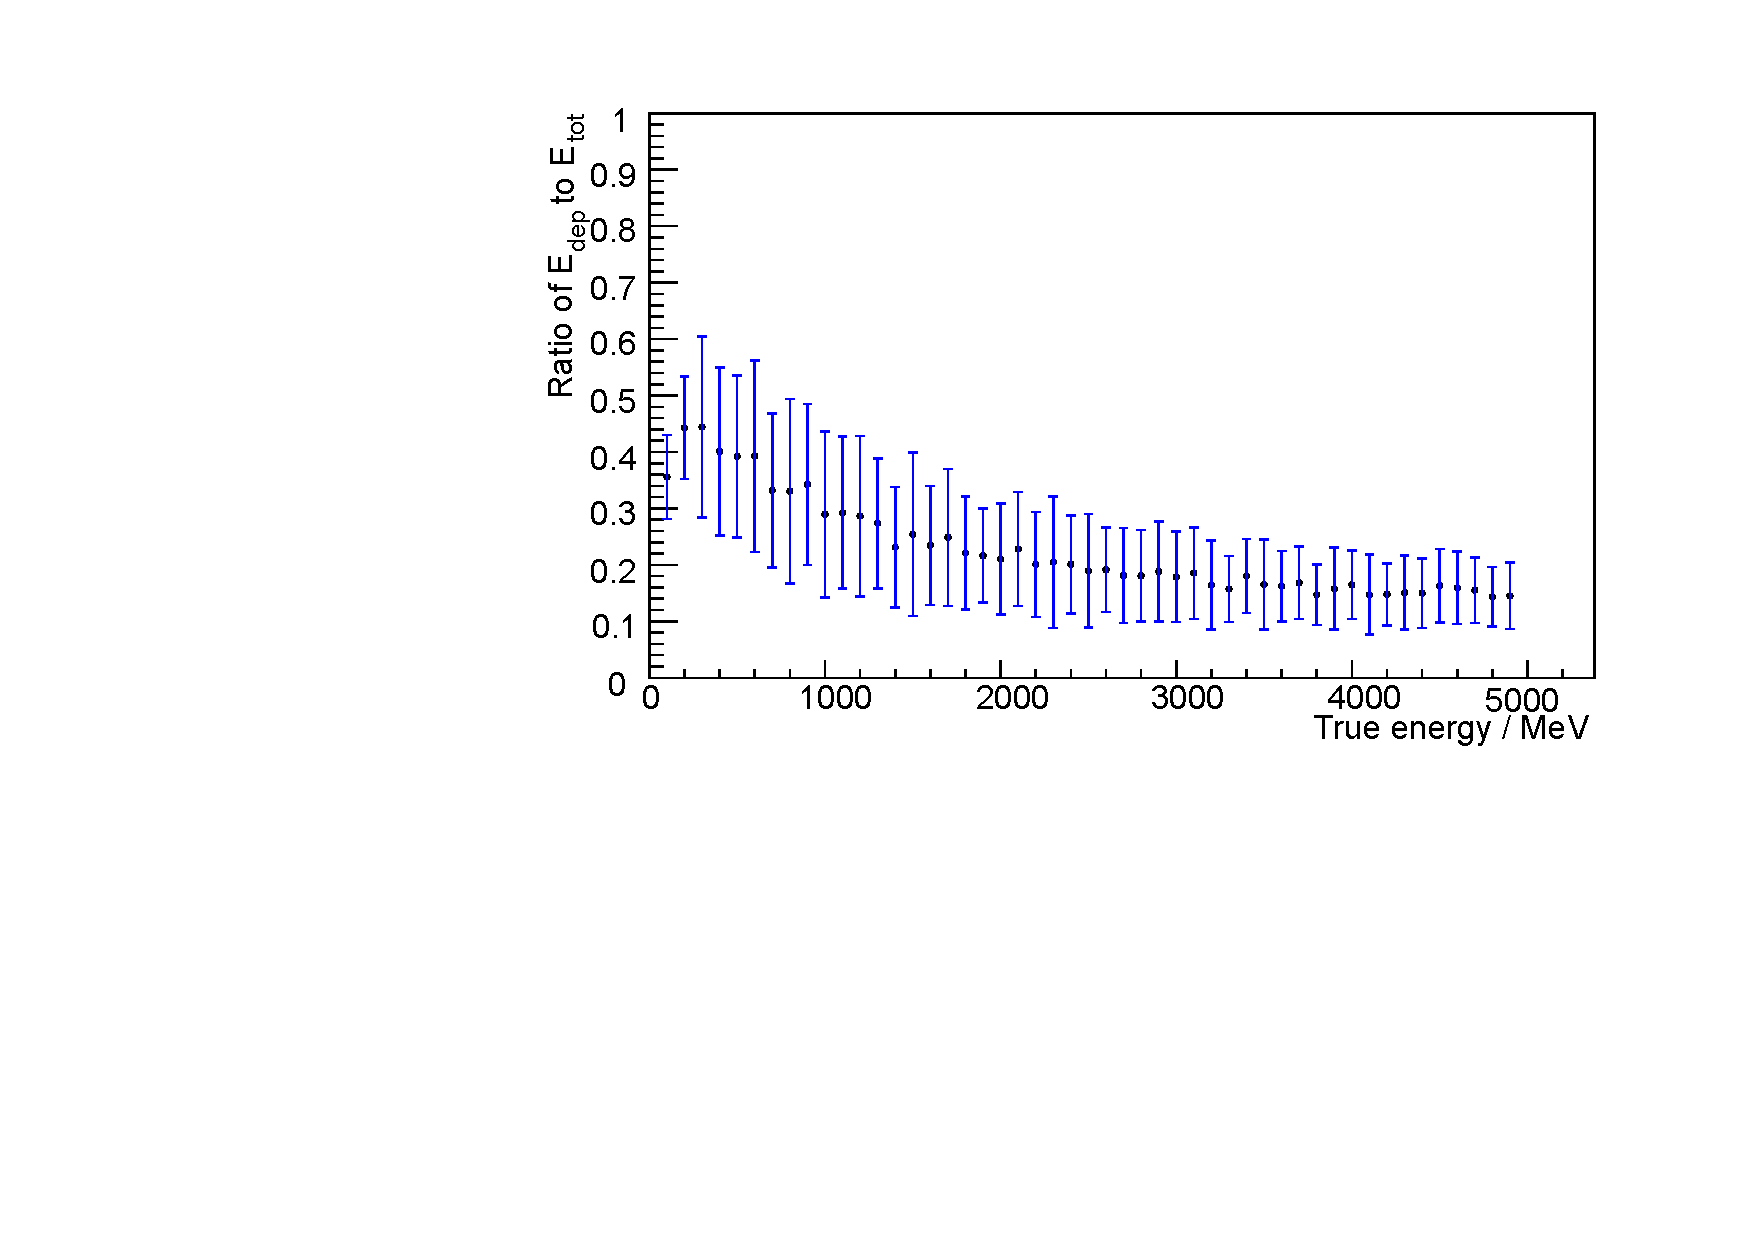
\includegraphics[angle=-90,width=0.45\textwidth]{chapters/detectorphysics_images/proton-energy-ratio}
    \label{fig:detector_energy_ratios_proton}
    }
\subfigure[Electron]{
    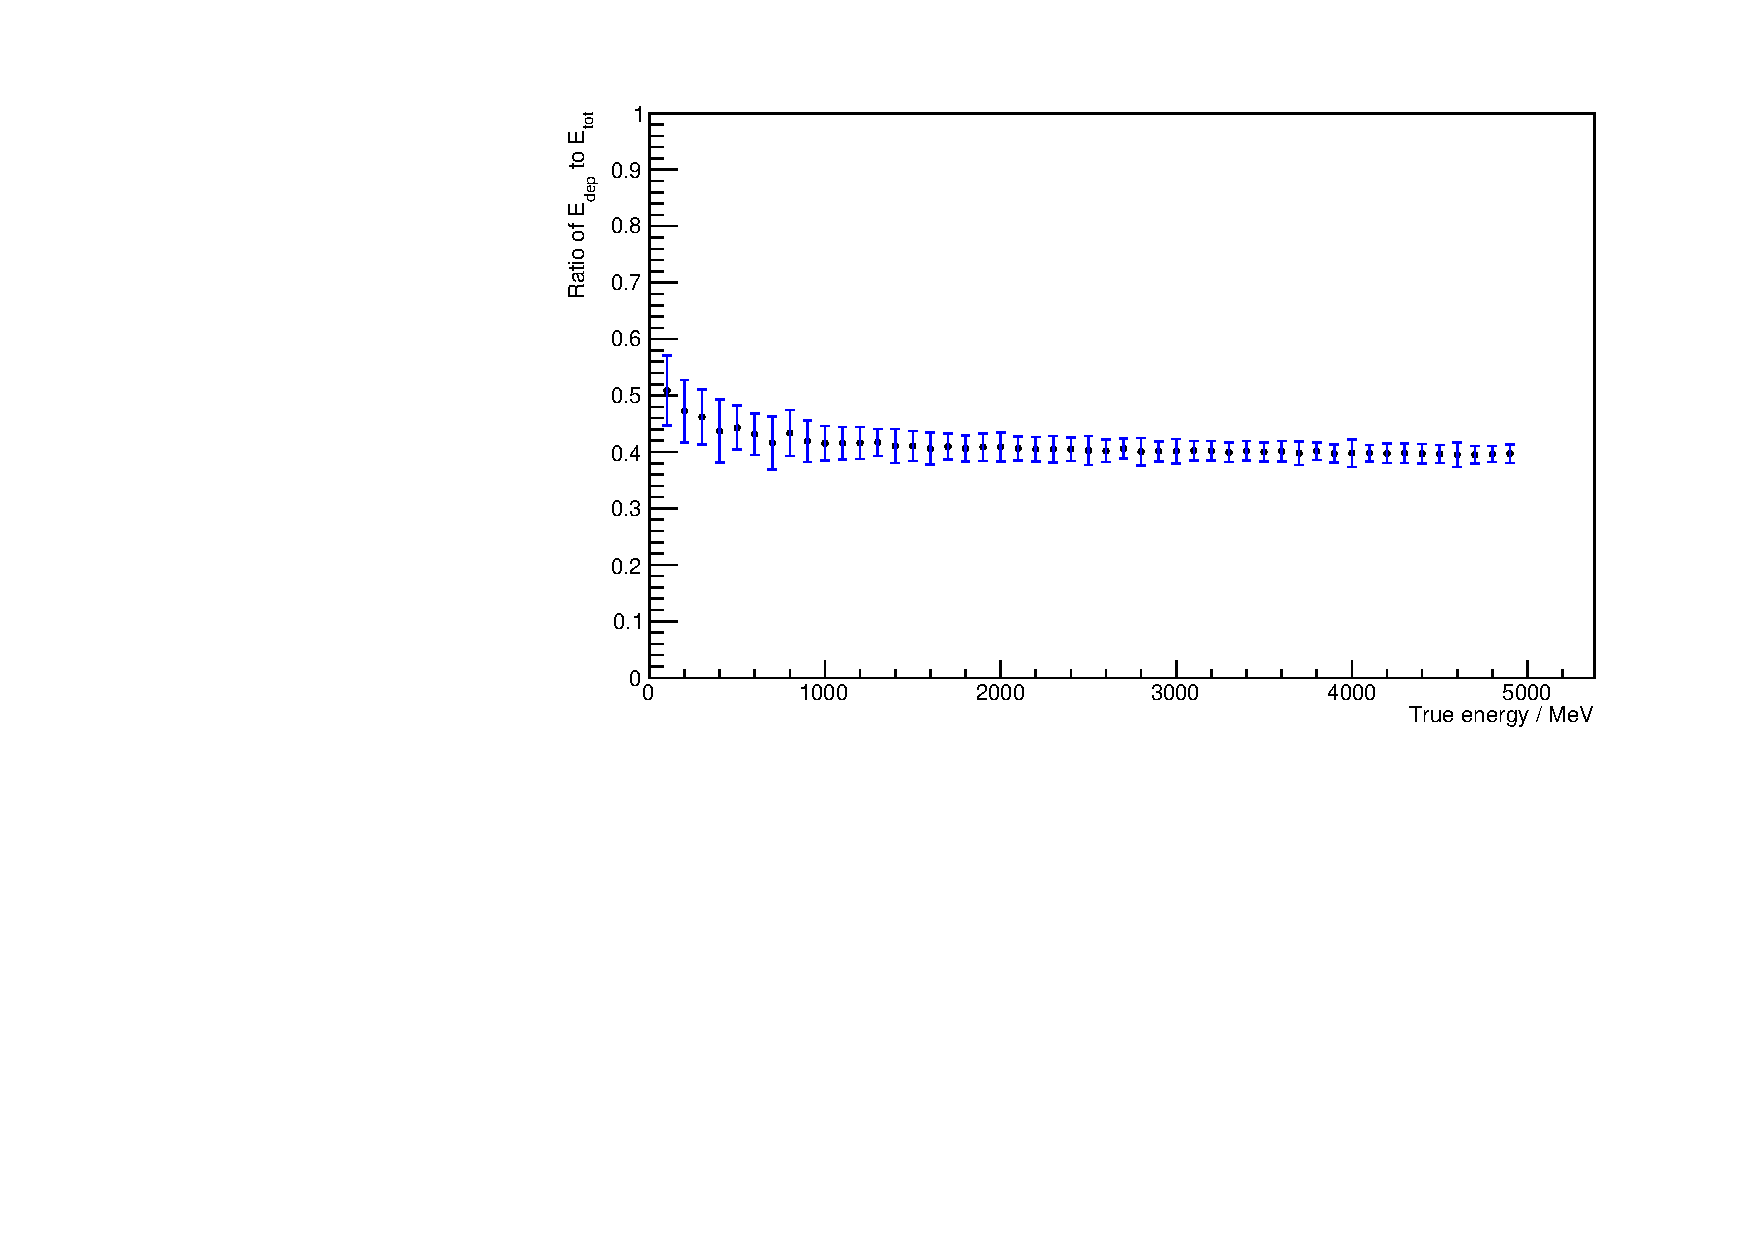
\includegraphics[angle=-90,width=0.45\textwidth]{chapters/detectorphysics_images/electron-energy-ratio}
    \label{fig:detector_energy_ratios_electron}
    }
\subfigure[Charged Pion]{
    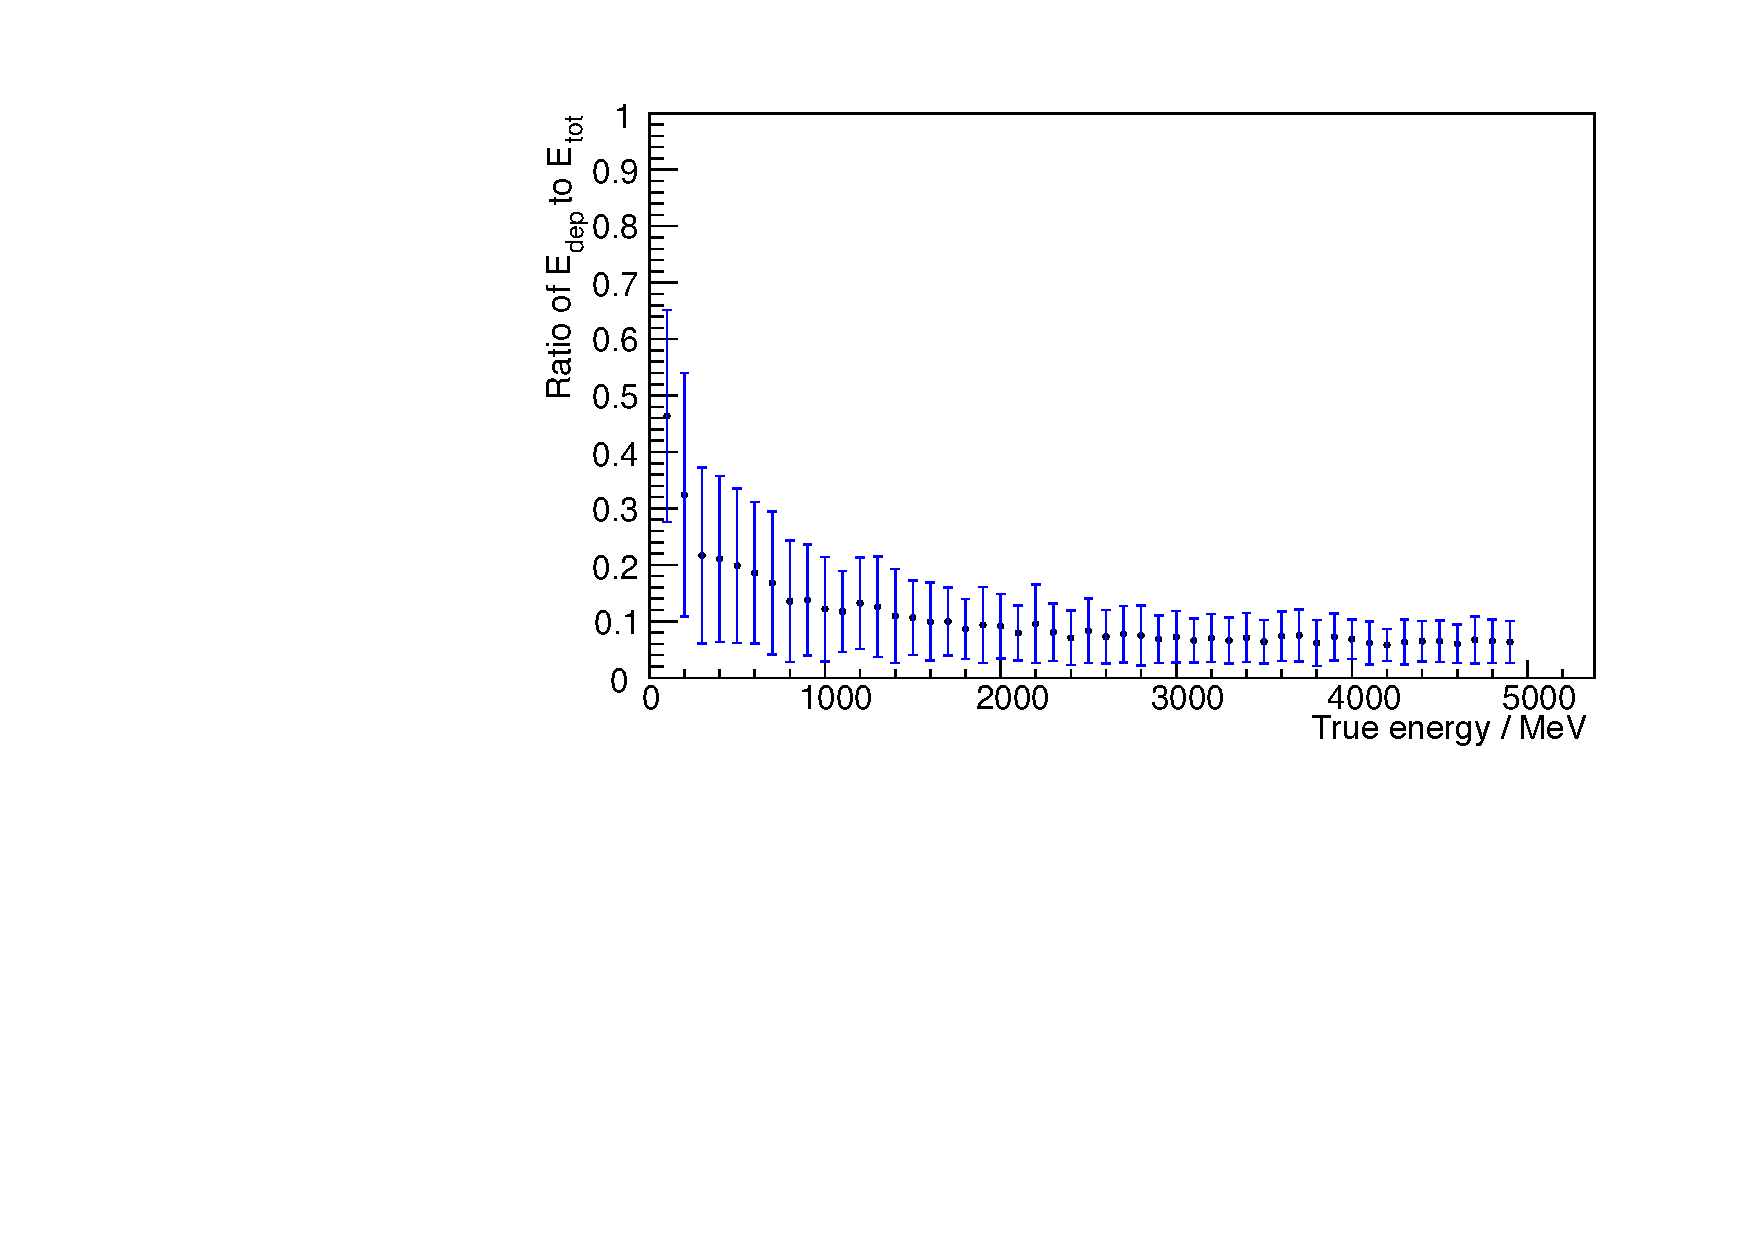
\includegraphics[angle=-90,width=0.45\textwidth]{chapters/detectorphysics_images/pi+-energy-ratio}
    \label{fig:detector_energy_ratios_charged_pion}
    }
\caption[Ratio of energy deposited to kinetic energy, by particle species]{\label{fig:detector_energy_ratios}Ratio of energy deposited in the Lamu simulation to the initial kinetic energy of the particle, by particle species (errors are statistical). See text for discussion.}
\end{figure}

\section{The TrackGen Toy Track Simulation}
In addition to the full physics simulation provided by Lamu (see section \ref{sec:lamu}), it is useful to be able to test algorithms for event reconstruction using simplified ``toy'' tracks. The TrackGen simulation is a Python program which produces events containing one or more straight line segments, tracked through cubic voxels with ``energy'' deposition $L\cdot dE/dx$ where $L$ is the length of the track segment through a voxel and $dE/dx$ is a constant `energy loss' per unit length for the track concerned. The calculated `energy' is deposited at the centre of each voxel. There is no attempt to model physics processes such as Bethe-Bloch energy loss or scattering. Similarly, no detector properties are taken into account. This produces very clean (but still voxellised) events which, in principle, can be used to test the baseline efficiency of a reconstruction algorithm without dealing with a combination of algorithm effects and physics effects.

The core of the TrackGen simulation deals with calculating the intersection of straight lines with a set of voxels, determining the segment length through a voxel, and keeping track of the energy deposits. It is possible to set the voxel size (as a parameter to the TrackGen program) but only cubic voxels are supported, i.e. a single side length is specified, rather than the more general three that would be required for arbitrary cuboid voxels. In addition to the core tracker, several event generator modules produce different sets of straight lines, corresponding to different event topologies of interest. The topologies of most relevance to the reconstruction of neutrino events are:

\begin{enumerate}
    \item Single straight line; corresponding to a muon track without scattering.
    \item Single line with kink; corresponding to a muon track with a single large scatter.
    \item Two lines originating at a vertex, with fixed opening angle; corresponding to an interaction vertex and e.g. $\ccqe$ final state.
    \item Multiple lines originating at a vertex; corresponding to a higher-energy $\nu$ interaction producing multiple final state particles.
\end{enumerate}

The TrackGen simulation has event generator modules for each of these topologies, producing events consisting of one or more straight line segments, each tracked through a voxellised space. Output is to an SQLite3~\citep{SQLite} database file with a simple table structure.

\section{Neutrino Event Generation with Genie}\label{sec:genie}
The Genie~\citep{Genie} neutrino event generator is used to generate sets of final state particles (including momenta) from the interactions of neutrinos of a given flavour on Argon nuclei at a variety of energies. These final state particles are fed into the Lamu simulation as input trajectories and tracked through a \ac{LAr} volume.

Genie allows for the selection of interaction type, e.g. \ac{CCQE} scattering, but it is recommended that users limit themselves to selecting only charged current or neutral current interactions, since there is not a one-to-one mapping between physical interaction and final state topology, and physicists are mostly concerned with final state topologies. For instance, when one talks about a \ac{CCQE} event, one typically thinks of a $\ccqe$ final state. The reality is that a $\ccqe$ final state can occur in a number of ways, with \ac{CCQE} interactions a major contributor. Furthermore, a \ac{CCQE} interaction can produce other final states, particularly if the resulting nucleon undergoes further interactions in the nucleus before emerging (see figure \ref{fig:feynman-cc} for illustration). For this reason, the events generated for this thesis using Genie were made by specifying only charged or neutral current interactions, without imposing limitations on the subtype of the interaction. The results were subsequently filtered to ``cherrypick'' the topologies of interest, and a note made of the fraction of the total events generated which passed the filter. In the remainder of this thesis, the term CCQE is used, for convenience, to mean ``\emph{charged current interactions producing a $\ccqe$ final state}''.

\begin{figure}
\centering
\subfigure{
    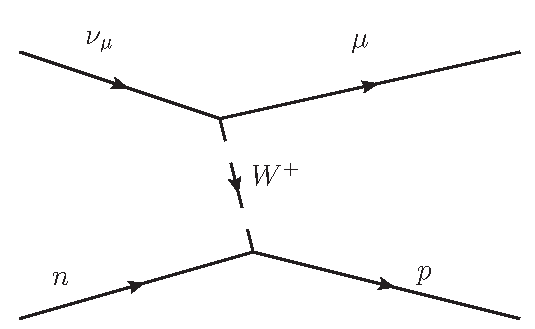
\includegraphics[width=0.45\textwidth]{chapters/detectorphysics_images/ccqe}
    \label{fig:feynman-ccqe}
}
\subfigure{
    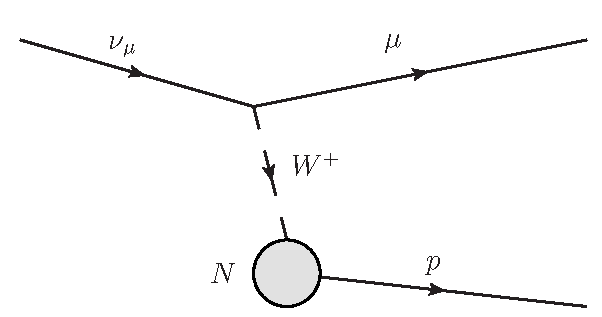
\includegraphics[width=0.45\textwidth]{chapters/detectorphysics_images/cc-mu-p}
    \label{fig:feynman-cc-mu-p}
}
\caption[Charged current neutrino interactions producing a $\ccqe$ final state]{\label{fig:feynman-cc}The difference between true charged current quasi-elastic (CCQE) interactions (left), and charged current interactions producing a $\ccqe$ final state (right). The left-hand diagram is included in the possibilities for the right-hand diagram, but in a more general sense any interaction could occur in the nucleus, and we see only the products that leave. Genie allows us to select events based on these products, leaving the details of the interaction that produced them to be decided by Genie itself.}
\end{figure}

\section{Neutrino Experiments Using Liquid Argon TPCs}
A number of existing and planned experiments use a \acs{LAr TPC}. This section summarises the main experiments, including notable prototypes or future planned experiments, describing the technology used in the detector, the status of any software framework, and the issues faced by those experiments.

\subsection{The Fermilab Liquid Argon Experiments}
A number of proposed and running experiments at Fermilab use \acs{LAr TPC}s. There is a software framework called \emph{LArSoft}, which will be shared by the ArgoNeuT~\citep{ArgoNeuT}, MicroBooNE~\citep{MicroBooNE} and LBNE~\citep{LBNE} experiments.

\subsubsection{The LArSoft Framework}
LArSoft aims to be a complete set of reconstruction, simulation and analysis tools, shared by the liquid Argon neutrino experiments based at Fermilab. It accepts data from GENIE and Geant simulations, as well as real data from the ArgoNeuT experiment. The development goals are to provide wire calibration, hit finding and clustering, endpoint finding, 3D tracking, 3D shower finding, vertex finding and calorimetry~\citep{LArSoft2011}. The sections below on each Fermilab experiment contain further details of the use of the LArSoft framework for their reconstruction tasks.

\subsubsection{ArgoNeuT}
ArgoNeuT~\citep{ArgoNeuT} is a small \acs{LAr TPC} exposed to the Fermilab NuMI (Neutrinos at the Main Injector) beam. ArgoNeuT is the first phase of Fermilab's path towards using a massive \acs{LAr TPC} in the LBNE experiment.

The detector itself consists of a vacuum-insulated cryostat holding $550$ litres of liquid Argon, with a \acs{TPC} active area of $40\times47\times90\cm^3$, or approximately $170$ litres. The maximum drift length is $47\cm$ and there is a uniform electric field of $500\volt\cm^{-1}$ between the cathode and the anode, which consists of three wire planes with $4\mm$ wire pitch in each plane and a $4\mm$ spacing between planes. Liquid Argon is circulated through a closed-loop cooling and filtration system which removes electronegative impurities.

The first (\emph{shield}) wire plane is not instrumented, and acts to shield the outer two planes from induced signals created by drifting electrons in the main \acs{TPC} volume. The second (\emph{induction}) plane consists of $240$ wires at $+60\degree$ to the beam axis. Drifting electrons induce a signal in these wires after passing the shield plane. The third (\emph{collection}) plane consists of $240$ wires at $-60\degree$ to the beam axis, and collects the electrons at the end of their drift.

At each beam spill, $2\times240$ signals are collected from the wires, pre-amplified, filtered and digitized. A wire-plane \emph{hit} is characterised by the peak signal amplitude and the coordinates in the (\emph{wire--time}) plane. Hits from both planes are reconstructed into space coordinates associated with the tracks of ionising particles through the drift volume and associated with the energy deposited at those coordinates.

The DBSCAN algorithm is used to cluster hits into tracks, using an elliptical neighbourhood based on the geometry of the wire planes. Lines are found in each 2D plane of clustered hits using the Hough transform, and those lines with similar slopes and connecting endpoints are merged together on a plane by plane basis. At this stage, candidate interaction points are found by looking at the longest 2D clusters in each plane. Some confusion is caused by $\delta$ rays, which must be filtered out.

Tracks found in each plane are combined into 3D by matching the drift coordinates of each hit and requiring that the hits coincide within a time window allowing for the drift time between planes. Geometric data is provided in the form of direction cosines and the effective length of the track portion that was exposed to a single wire. This allows for the computation of $dE/dx$ information, which is corrected using Birk's model for electron recombination.

\subsubsection{MicroBooNE}
The MicroBooNE~\citep{MicroBooNE} experiment has three primary objectives; to resolve the source of the MiniBooNE low energy excess,\footnote{MiniBooNE saw a $3\sigma$ excess of events producing low energy $e^-$ or $\gamma$ final states~\citep{MiniBooNE}.} to measure a variety of neutrino cross-sections, and to provide technical experience in the construction and operation of a large \acs{LAr TPC} in preparation for LBNE and future experiments.

The detector will consist of a $2.325\times 2.5604 \times 10.368 \metre^3$ liquid Argon volume with the longest dimension along the beam. The readout will consist of wire planes on a $3\mm$ wire pitch and with $3\mm$ separation, operating in a configuration similar to ArgoNeuT. A drift field of $500\volt\cm^{-1}$ will be applied across the $61.8\metre^3$ drift volume (approximately $86$ tonnes of liquid Argon). Pre-amplification and pulse shaping will be performed inside the cryostat with cold electronics, before further amplification stages outside the cryostat, leading to the eventual digitisation of the pulses.

The offline software for MicroBooNE uses the LarSoft toolkit, and includes a simulation using Geant4. The first stages of reconstruction calibrate the wire signals and localise them into spatial hits. These are grouped into clusters, then further grouped into \emph{prongs}, which represent either tracks or showers. Vertex finding proceeds by looking for prongs originating from a common point. The clustering is performed in two dimensions (wire-plane projections) using DBSCAN and edge or vertex finding algorithms based on the Harris function (see chapter \ref{sec:two-dim-feature-detection}). Track finding is performed in 2D using the Hough transform, with matched lines being combined into 3D tracks. LarSoft does not currently provide a way to perform full three-dimensional track reconstruction without first using two-dimensional projections.

MicroBooNE faces a number of challenges during the construction and operation, including the readout of a large number of wire channels in cryogenic environments, maintaining liquid Argon purity in a large detector without resorting to vacuum processes, ensuring that wires do not break inside the large cryostat volume, and demonstrating successful simulation and reconstruction of events in a large \acs{LAr TPC}.

\subsubsection{LBNE}
The LBNE~\citep{LBNE} collaboration aim to build a long baseline neutrino oscillation experiment using a large \acs{LAr TPC} as the far detector. With a $1300\km$ baseline and an intense neutrino beam providing neutrino energies between $0.5\GeV$ and $5.0\GeV$, the aim is to make precision measurements of $\theta_{13}$ and to determine the $\Charge\Parity$ violating phase $\delta_{CP}$ using a combination of traditional near detectors at Fermilab, and a $10\kton$ \acs{LAr TPC} far detector.

The \acs{LAr TPC} will consist of two cryostats built side-by-side, with their long axes parallel to the beam, and separated by a wall which is centered on the beam centre. Each cryostat will be $13.9\times 14\times 25.3\metre^3$ and have a fiducial mass of $5\kton$ or a total mass of $6.7\kton$ (giving $13.5\kton$ for the entire far detector).

The TPC itself will consist of alternating rows of anode and cathode planes with a uniform electric field of $500\volt\cm^{-1}$ in the drift spaces. The maximum drift distance (i.e. the separation of the planes) is $2.3\metre$, and the cathode will consist of three instrumented wire planes (two induction and one collection) and a fourth, uninstrumented, plane to shield the others from electrostatic discharge and improve signal-to-noise ratio on the first induction plane. The planes will be oriented vertically and at $\pm45\degree$ to the vertical, improving resolution along the beam compared to the $\pm60\degree$ configuration of ArgoNeuT and MicroBooNE, and will have a $4.5\mm$ wire pitch. With $2650$ wires in each cathode plane, there will be a total of $153600$ readout channels per cryostat. Readout electronics will be in the liquid Argon, and will include pre-amplification, pulse shaping and digitisation.

LBNE will use the LArSoft framework and take advantage of the reconstruction procedures demonstrated by both ArgoNeuT and MicroBooNE.

\subsection{Laguna LBNO}

\subsubsection{Detector Design}
\subsubsection{Software Framework}

\subsection{Icarus}
The Icarus T600 detector is a $600\ton$ \acs{LAr TPC} operating at the Gran Sasso National Laboratory in the CNGS (CERN to Gran Sasso) neutrino beam. It has three readout wire planes, at $0\degree, +60\degree$ and $-60\degree$ to the vertical, all with a $3\mm$ wire pitch.

The first stage of reconstruction consists of converting individual wire signals into hits by recording their spatial position and calorimetric information. These are clustered into 2D structures in each wire plane, which are categorised as tracks or showers. The DBSCAN algorithm has been proposed for this clustering.

Three-dimensional reconstruction is performed by matching clusters in at least two 2D planes, there is no fully three-dimensional reconstruction at present.



\chapter{The Latte Framework}\label{chapter:Latte}

\section{Introduction}
The Latte framework forms the software basis for almost all of the reconstruction algorithms described in this thesis. It acts as both a set of utilities and a unifying central control mechanism. This chapter discusses several of the algorithms provided, ending with an overview of the control structures of the Latte framework itself. Some components of Latte form a significant contribution to the work in this thesis, and are discussed separately in subsequent chapters.

\section{Nearest Neighbour Search using \acs{KDTree}}\label{sec:latte_kdtree}
The \ac{KDTree} is a data structure for partitioning a $k$-dimensional space by representing the points as nodes in a binary tree. Using a \ac{KDTree} it is possible to perform nearest-neighbour search in $O(\log N)$ time\citep{Bentley1975},\footnote{$N$ is the number of data points to be partitioned. The KDTree itself is built in $O(kN\log N)$ time.} compared with the brute-force search complexity of $O(N^2)$. An introductory tutorial on \aclp{KDTree} appears in \citep{Moore1991}. The \ac{KDTree} is not a clustering algorithm, but its rapid near-neighbour search forms a central part of several clustering algorithms, as well as being used for the charge weighting procedure (see chapter \ref{sec:cellularautomaton_charge_weighting}) and the cell generation (chapter \ref{sec:cellularautomaton_cell_generation}) stage of the \acl{CA} track reconstruction procedure.

The implementation currently used is that of the \emph{SciPy}\citep{SciPy} library of Python code for scientific computing.

\section{Charge Weighting}\label{sec:cellularautomaton_charge_weighting}
Data from a \ac{LAr TPC} is assumed to be in the form of $(x, y, z)$ voxels with an associated charge deposit $Q$. The voxel shape is determined entirely by the readout mechanism; a 2D readout plane determines the $xy$ resolution while the readout sampling rate determines the $z$ resolution as expected for a \ac{TPC}. This structure is retained in the Geant4 simulation through the use of cubic voxels with a side length of $1\mm$. In order to transform this data into a representation more closely resembling the true passage of ionising radiation through the detector, a charge weighting procedure is applied. This procedure adjusts the spatial coordinates of each charge deposit (voxel) by taking the charge-weighted average of the spatial coordinates of all hits within a sphere of some radius (default: $2\mm$) centered on that voxel:

\begin{equation}\label{eqn:charge_weighted_avg_position}
	\vec{x}^\prime = \frac{\displaystyle \sum_i \vec{x}_i Q_i}{\displaystyle \sum_i Q_i}
\end{equation}

The neighbouring hits are discovered using the \ac{KDTree} algorithm described in section \ref{sec:latte_kdtree}.

Charge weighting\footnote{This is not, strictly speaking, the usual definition of charge weighting, in which a set of hits is reduced to a smaller set of charge-weighted hits, but more of a smoothing process to reduce the geometric effects of the readout system. Hits are retained here primarily to facilitate accessing truth information.} in this way moves the position of each charge deposit closer to the local charge cloud, bringing track-like charge deposits closer to a straight line (see figure \ref{fig:ca_charge_weighting}). For each point, the sum is taken over the unweighted positions of neighbours and a new dataset is generated, containing the weighted positions. This results in a stable, deterministic output.

\begin{figure}
\centering
\subfigure[Hits as central points of voxels]{
	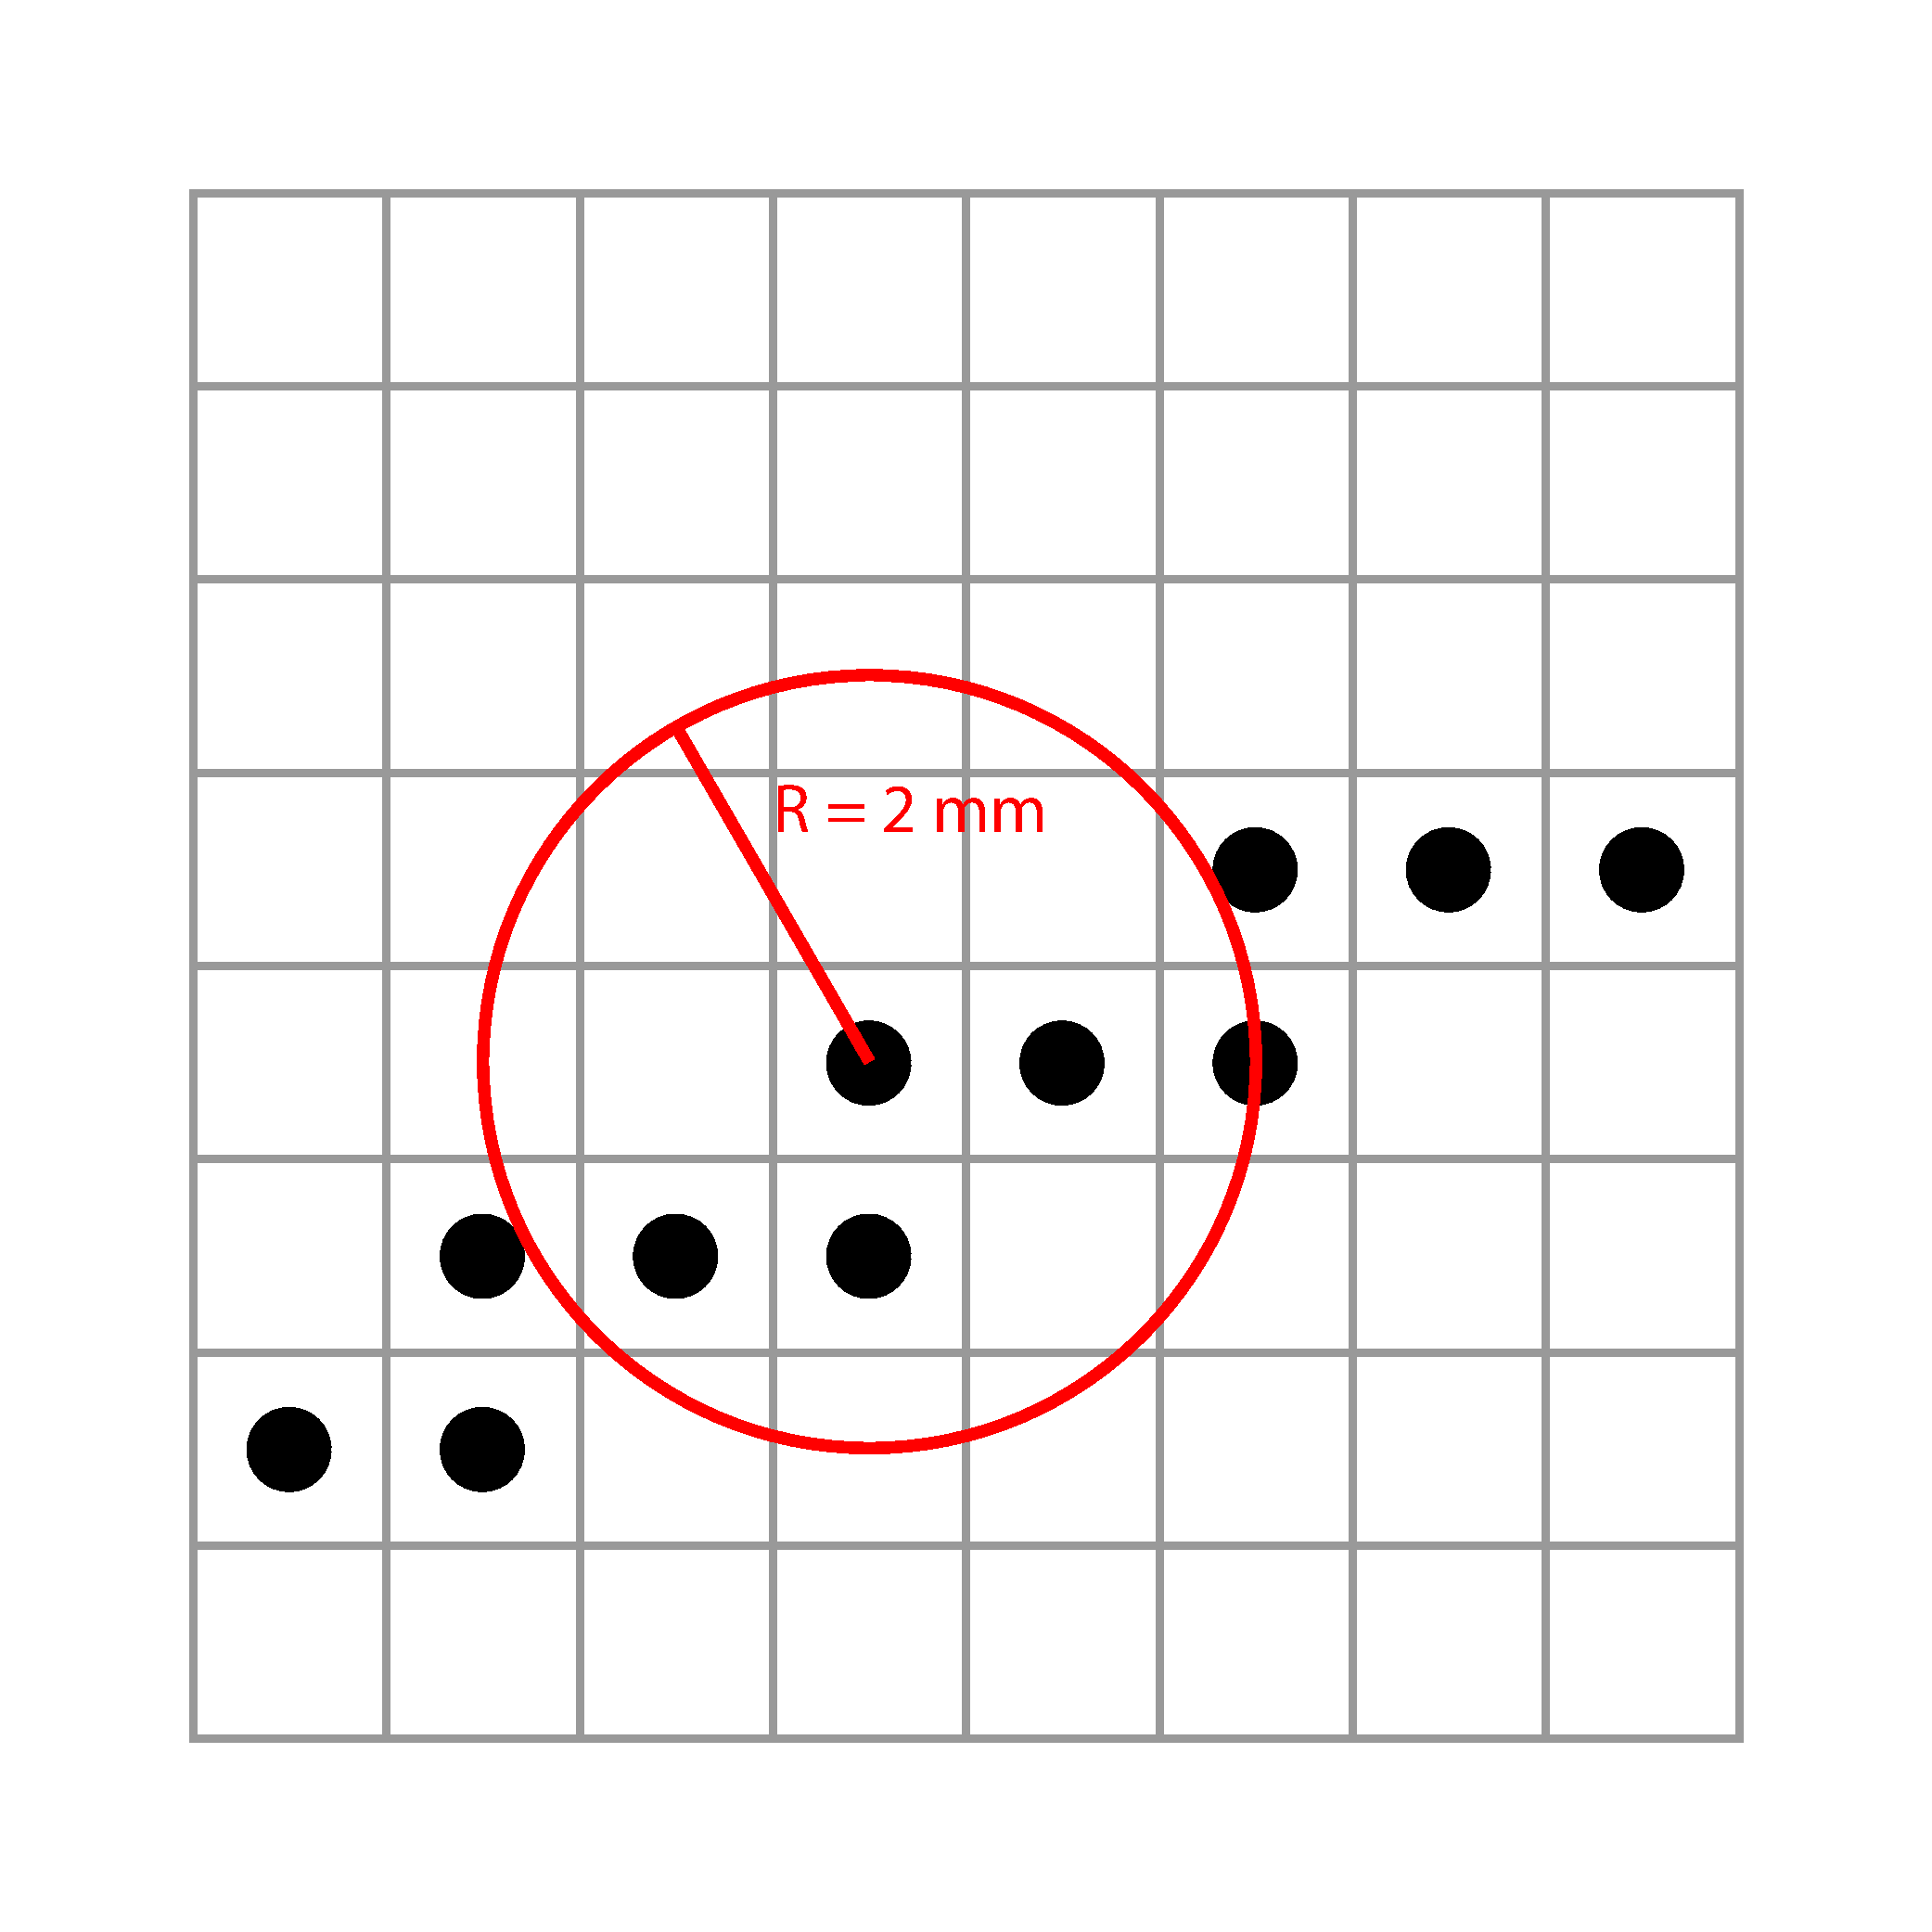
\includegraphics[width=0.4\textwidth]{chapters/cellularautomaton_images/ChargeWeighting1}
	\label{fig:ca_charge_weighting_1}
}
\subfigure[Hits shifted from voxel centres]{
	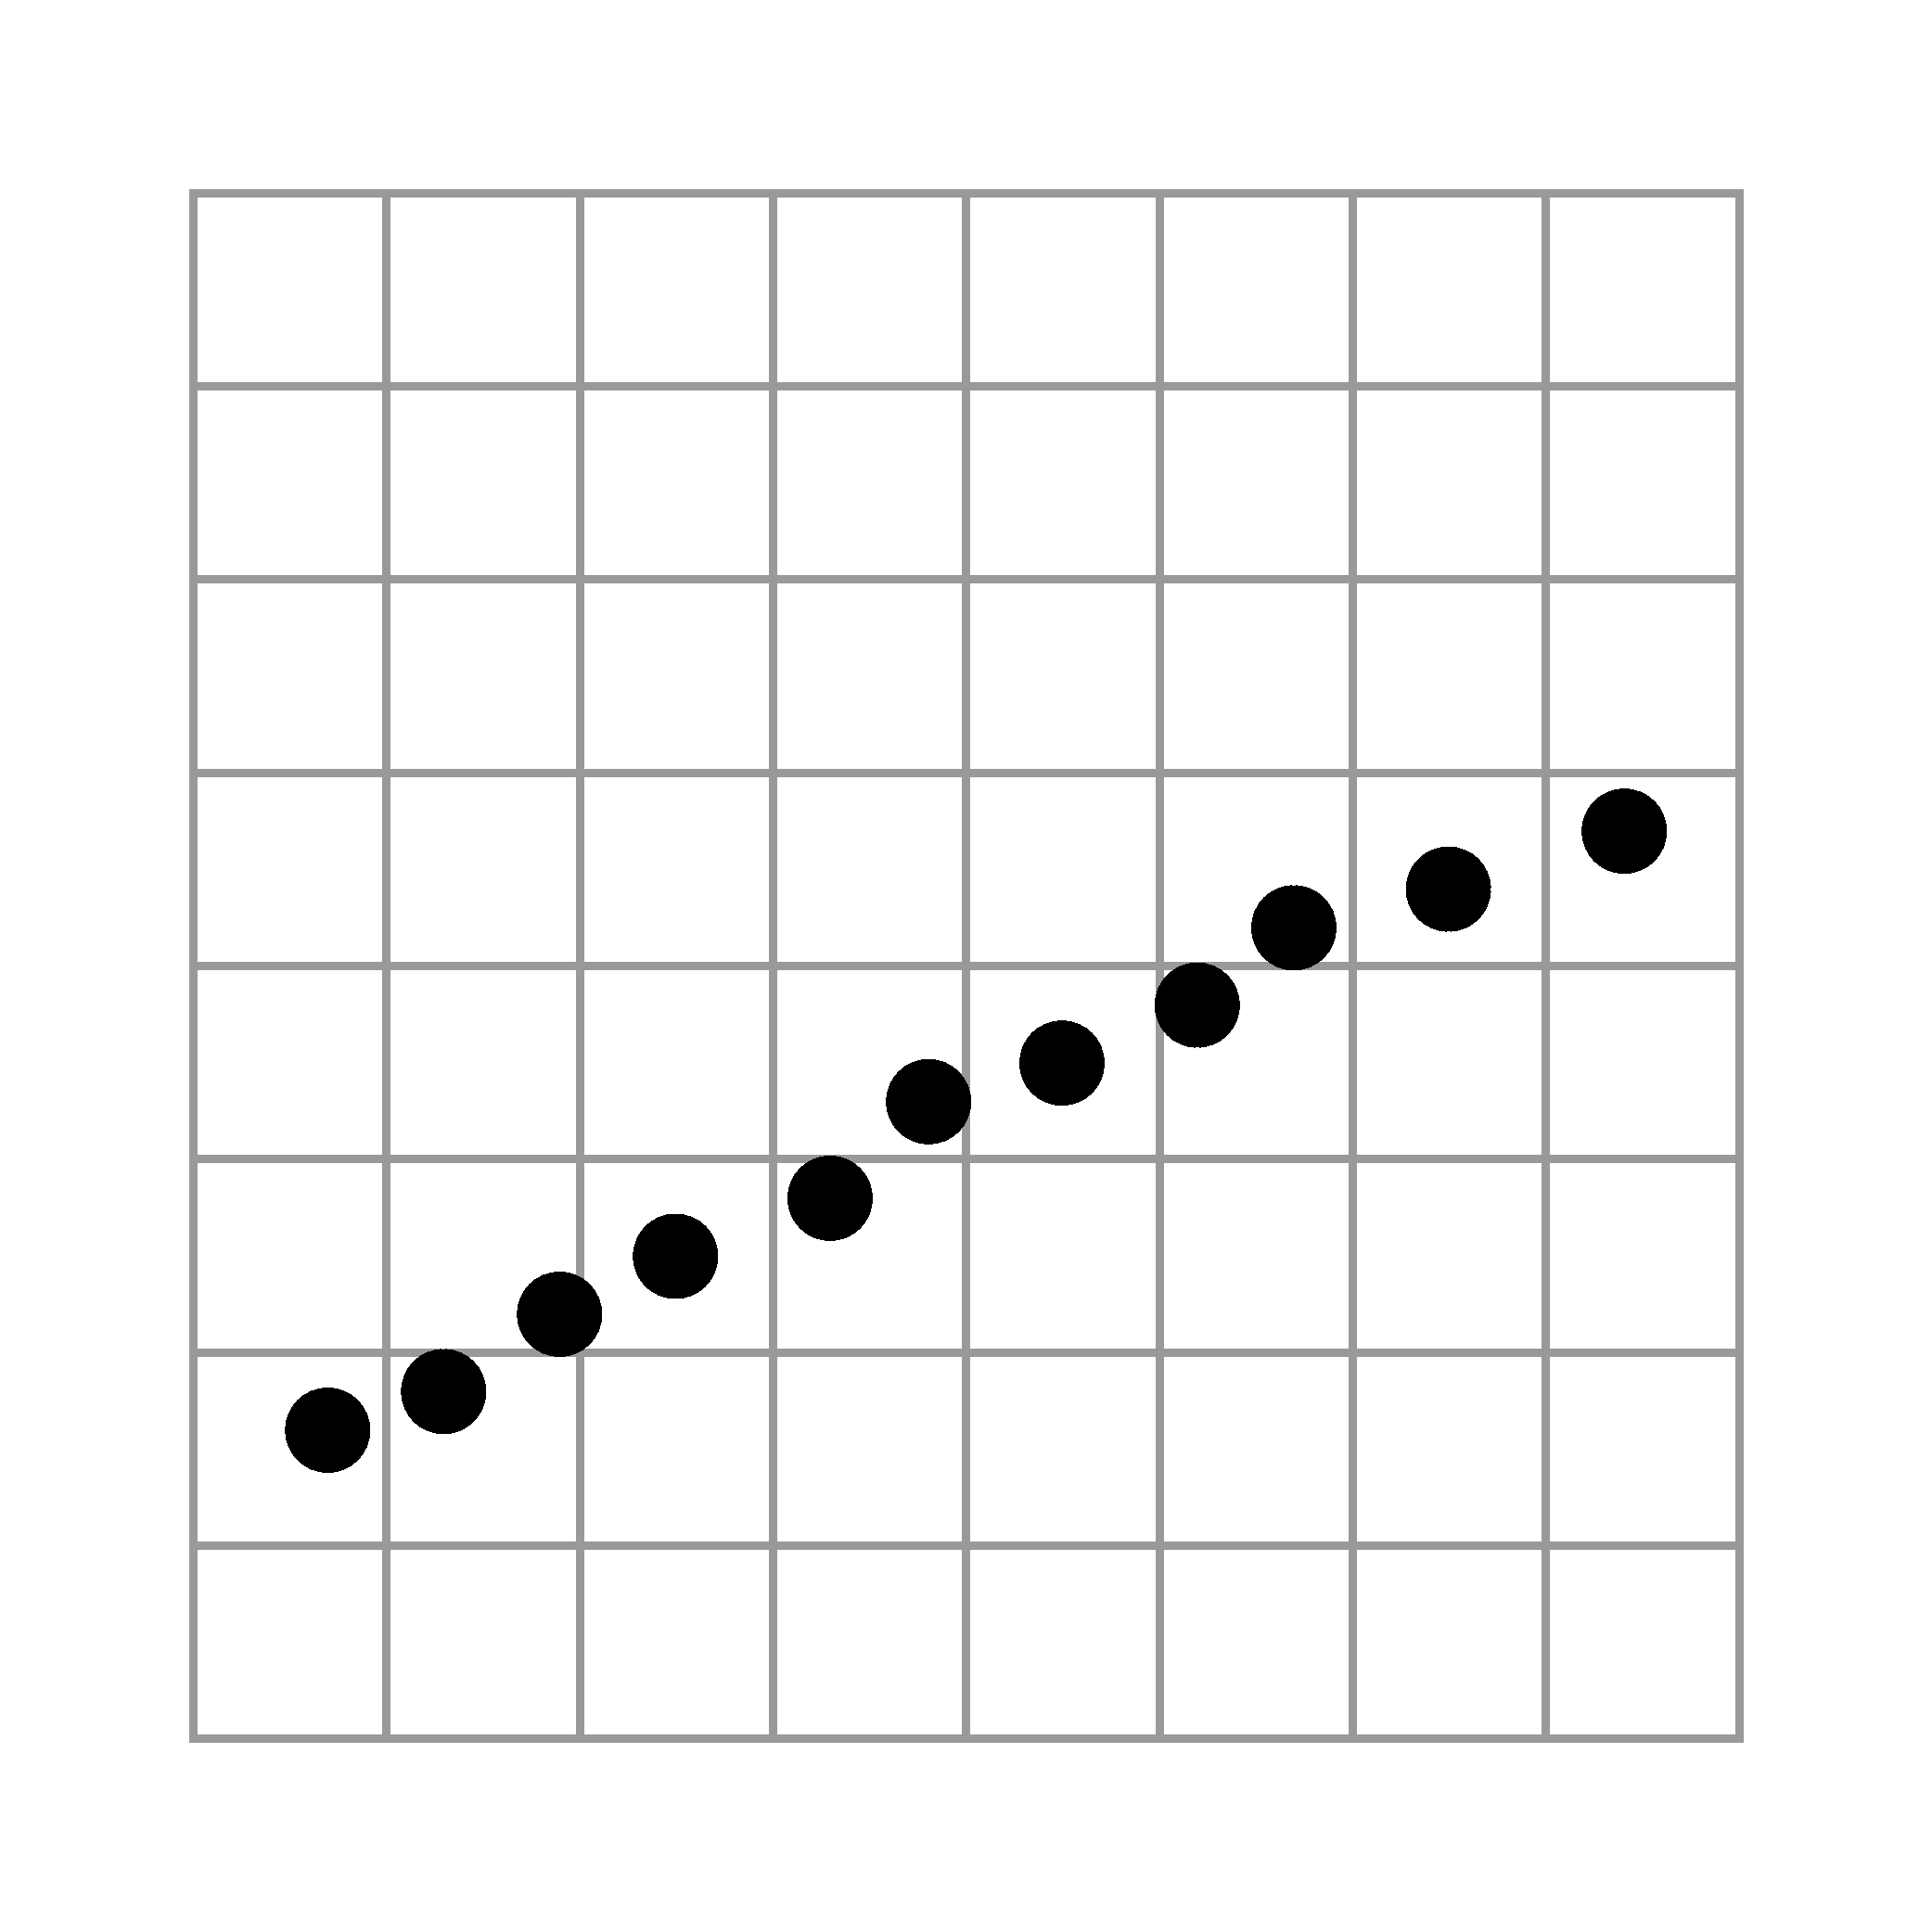
\includegraphics[width=0.4\textwidth]{chapters/cellularautomaton_images/ChargeWeighting2}
	\label{fig:ca_charge_weighting_2}
}
\caption[Diagram of the effect of charge weighting on hit position]{\label{fig:ca_charge_weighting}Schematic diagram of the effect of the charge weighting procedure on hit positions. In \subref{fig:ca_charge_weighting_1} each hit is positioned at the centre of a voxel. In \subref{fig:ca_charge_weighting_2} the hit positions have been adjusted based on the charge-weighted positions of surrounding hits within a $2\mm$ radius; this shifts them from the voxel centres and out of a regular grid structure.}
\end{figure}

\section{Density-based Clustering}
\subsection{\acs{DBSCAN}}\label{sec:latte_dbscan}
The \ac{DBSCAN} algorithm was proposed in 1996 as a means for clustering spatial data based on the varying densities of point clouds\citep{Ester1996}. The algorithm is characterised by its requirement that, for the neighbourhood $\epsilon$ around a given point in the cluster, the number of points $N$ in $\epsilon$ must exceed some threshold value $N_\mathrm{min}$. In this manner, the clustering is determined by identifying areas of high point density. Areas of low point density (i.e. any points not clustered) are identified as \emph{noise} and clustered together as such.

The \ac{DBSCAN} algorithm has been applied to spatial data obtained from a \ac{LAr TPC} by the ArgoNeuT experiment\cite{Spitz2011} to identify clusters in two 2D views, which are subsequently recombined into 3D based on wire readout timing information.

\ac{DBSCAN} has two configurable parameters; $\epsilon$, the radius around a given point within which neighbours must lie, and $N_\mathrm{min}$, the minimum number of those neighbours for a point to be considered part of a dense cluster. While these parameters can be optimised, they remain global, and \ac{DBSCAN} will not typically identify regions of changing density and cluster accordingly. This tends to result in a \ac{DBSCAN} clustering which wraps around the vertex of charged-current neutrino events (for example).

\subsection{\acs{OPTICS}}
The \ac{OPTICS} algorithm\citep{Ankerst1999} extends \ac{DBSCAN} by performing a \emph{hierarchical clustering}; an ordering operation which is equivalent to returning the density-based clusterings associated with a broad range of values of the parameter $\epsilon$. For example, given a fixed value of $N_\mathrm{min}$, clusters obtained with a small $\epsilon$ (that is, high density clusters) are completely contained within the clusters obtained for a larger $\epsilon$ (lower density). \ac{OPTICS} exploits this relationship to provide information about the clustering on all $\epsilon$ scales, allowing clusters to be extracted from spatial data with varying densities.

\section{Feature Detection}\label{sec:latte_feature_detection}
Feature detection refers to the procedure of locating interest points within an image or event. Latte provides two-dimensional feature detection using the method described in \citep{Morgan2010}. Three-dimensional feature detection is currently based on running the two-dimensional feature finder in multiple projections and combining the results.

\subsection{Two-dimensional Feature Detection}
Two-dimensional feature detection uses the \emph{structure tensor} $S$, which is a second-moment matrix defined in terms of the intensity variation of a two-dimensional image:\citep{Morgan2010}
\begin{equation}\label{eqn:structure_tensor}
    S(x,y) = g(\sigma_s) \ast \left[ \begin{array}{cc} I_x(x,y)^2 & I_x(x,y)I_y(x,y) \\ I_x(x,y)I_y(x,y) & I_y(x,y)^2 \end{array} \right]
\end{equation}
where $\ast$ represents convolution, and $I_x(x,y)$ is the partial derivative of the image with respect to $x$ (similarly for $I_y(x,y)$). A Gaussian window $g(\sigma_s)$ is defined as
\begin{equation}\label{eqn:feature_det_gaussian_window}
    g(\sigma) = exp\left( \frac{-(x^2 + y^2)}{2\sigma^2} \right)
\end{equation}
and is used for averaging, as well as noise-reduction.

The eigenvectors and eigenvalues of $S(x,y)$ describe \emph{local} intensity variations within the image. Functions of $S(x,y)$ can therefore be constructed such that their local maxima correspond to features of a desired type. For example, the `V'-like corner of a particle decay vertex will have large intensity changes in all directions. Since it is this type of feature that we are interested in, the F\"orstner-Noble response function $R_N(x,y)$ is used within Latte:
\begin{equation}\label{eqn:forstner-noble}
    R_N(x,y) = \left\{ \begin{array}{cl} \frac{\det S}{\tr S} & \mathrm{if~} \tr S > 0 \\ 0 & \mathrm{if~} \tr S = 0 \end{array} \right.
\end{equation}

This function has local maxima at corner-like features, so the coordinates of these structures correspond to interest points such as decay vertices, interaction points and track endpoints; an example is shown in figure \ref{fig:feature-response}. Note that the feature detection service is used to provide the rough spatial location of a feature that warrants further investigation, and should not be used for precision operations such as vertex fitting.

\begin{figure}
    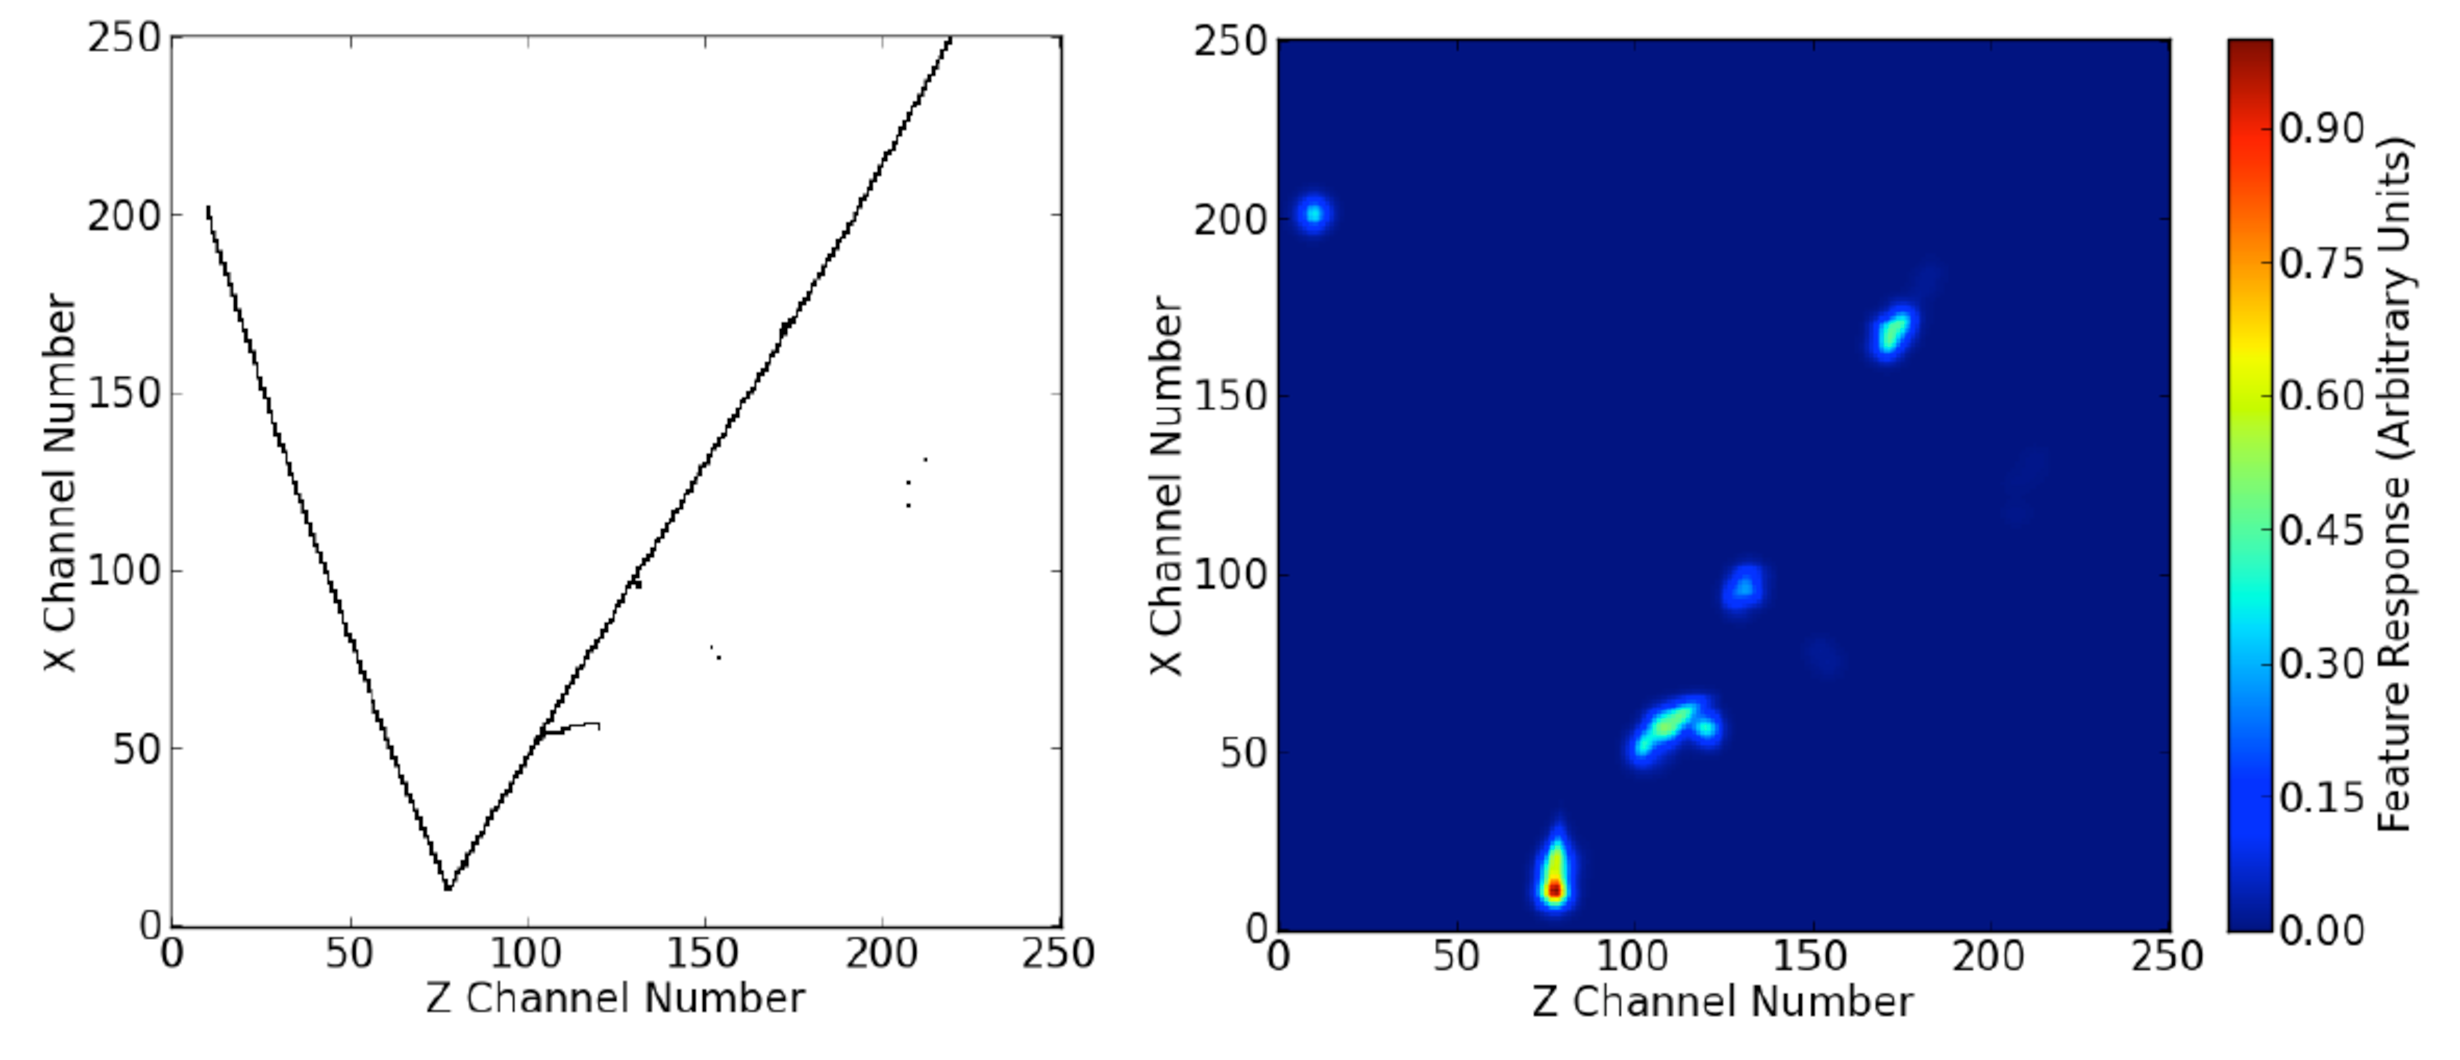
\includegraphics[width=\textwidth]{chapters/latte_images/feature-response}
    \caption[Feature response for a typical neutrino event]{\label{fig:feature-response}A typical neutrino event and the feature response as determined by the feature detection algorithm. The initial vertex and track endpoints are clearly visible, as well as several sites along the right (muon) track where delta electrons were produced.}
\end{figure}

\subsection{Three-dimensional Feature Detection}
Three-dimensional feature detection follows the algorithm outlined below, which uses multiple passes over two-dimensional projections.
\begin{enumerate}
    \item Run 2D feature detection in each of $xy$, $xz$ and $yz$ projections.
    \item Match interest points from each 2D run by requiring a shared coordinate (within some tolerance), e.g. features at $(1,0)$ in $xy$ and $(1,3)$ in $xz$ would be matched.
    \item For each such matching, make a new 3D feature using the information from both points, e.g. for the features above, create a feature at $(1,0,3)$ in $xyz$.
    \item Merge together features in 3D which are within some radial tolerance of each other. This deals with the potential duplicates which may be produced when a feature is visible in all three projections.
    \item Return a list of 3D features which survive the previous steps.
\end{enumerate}

Three-dimensional feature detection implemented in this way is imperfect, since we throw away information from one dimension in each projection, only to recombine the results later. A better approach would be to extend the mathematical definition of the structure tensor, $S$, to 3D (which is trivial) and define a new response function $R_N$ which yields a scalar having large values for corner-like features, and small values elsewhere (which is not trivial).

Despite this limitation, the three-dimensional feature response performs remarkably well. Figure \ref{fig:feature_3d} shows three performance metrics for feature detection applied to 1000 \ac{CCQE} neutrino interactions resulting in a $\mu^{-} + p$ final state. The total number of features found in an event is typically small, with between zero and two features found in most events. For the features found, the displacement from the true interaction vertex is typically small, though this has a long tail all the way to $1000\mm$, which is the radius of the detector used in this simulation. Finally, the normalised response at the true vertex is typically close to $1$, where normalised response is the response at a given feature, divided by the largest response value in the entire event. These characteristics apply even though delta electrons are a large source of noise, having typically high feature response values and appearing throughout the spatial extent of the event.

\begin{figure}
\centering
\subfigure[ ]{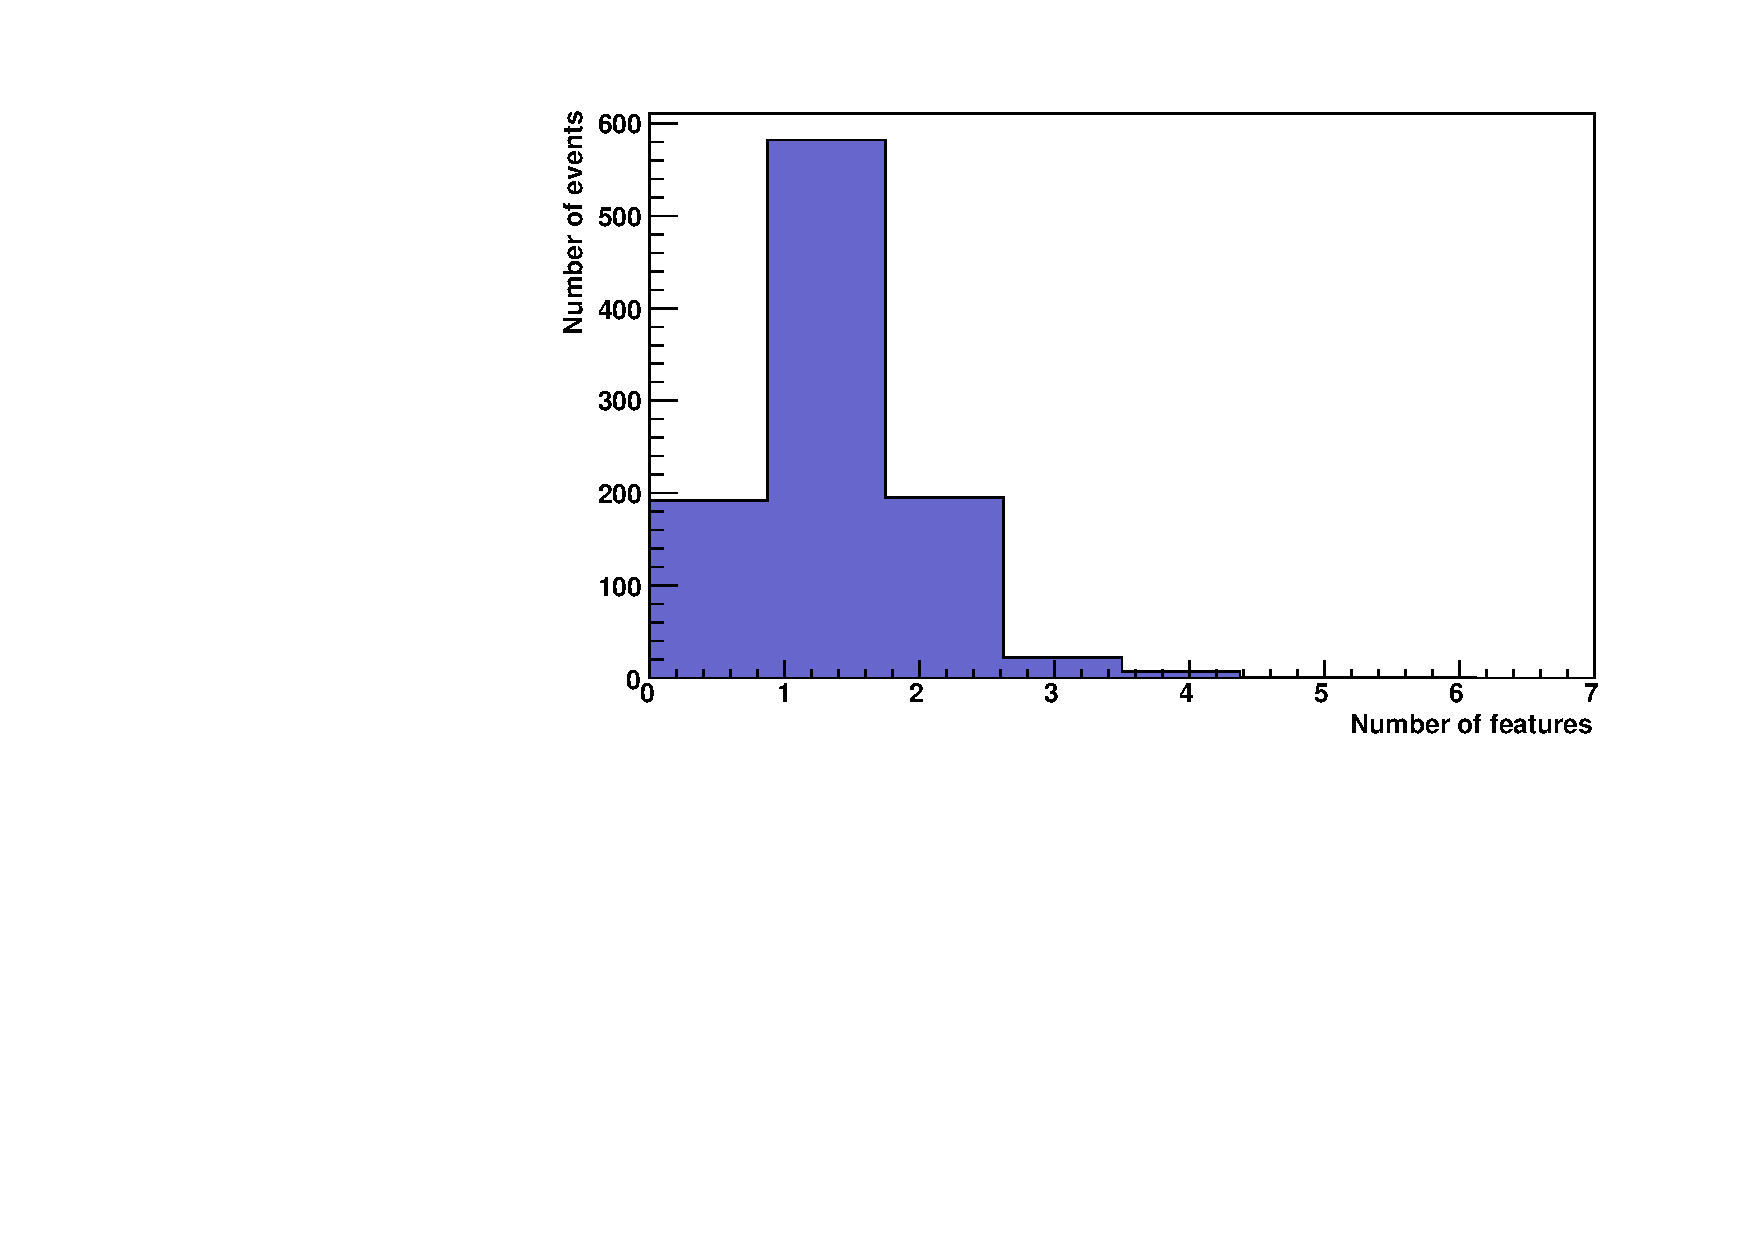
\includegraphics[width=0.35\textwidth,angle=-90]{chapters/latte_images/feature-counts-qel}\label{fig:feature_3d_counts}}
\subfigure[ ]{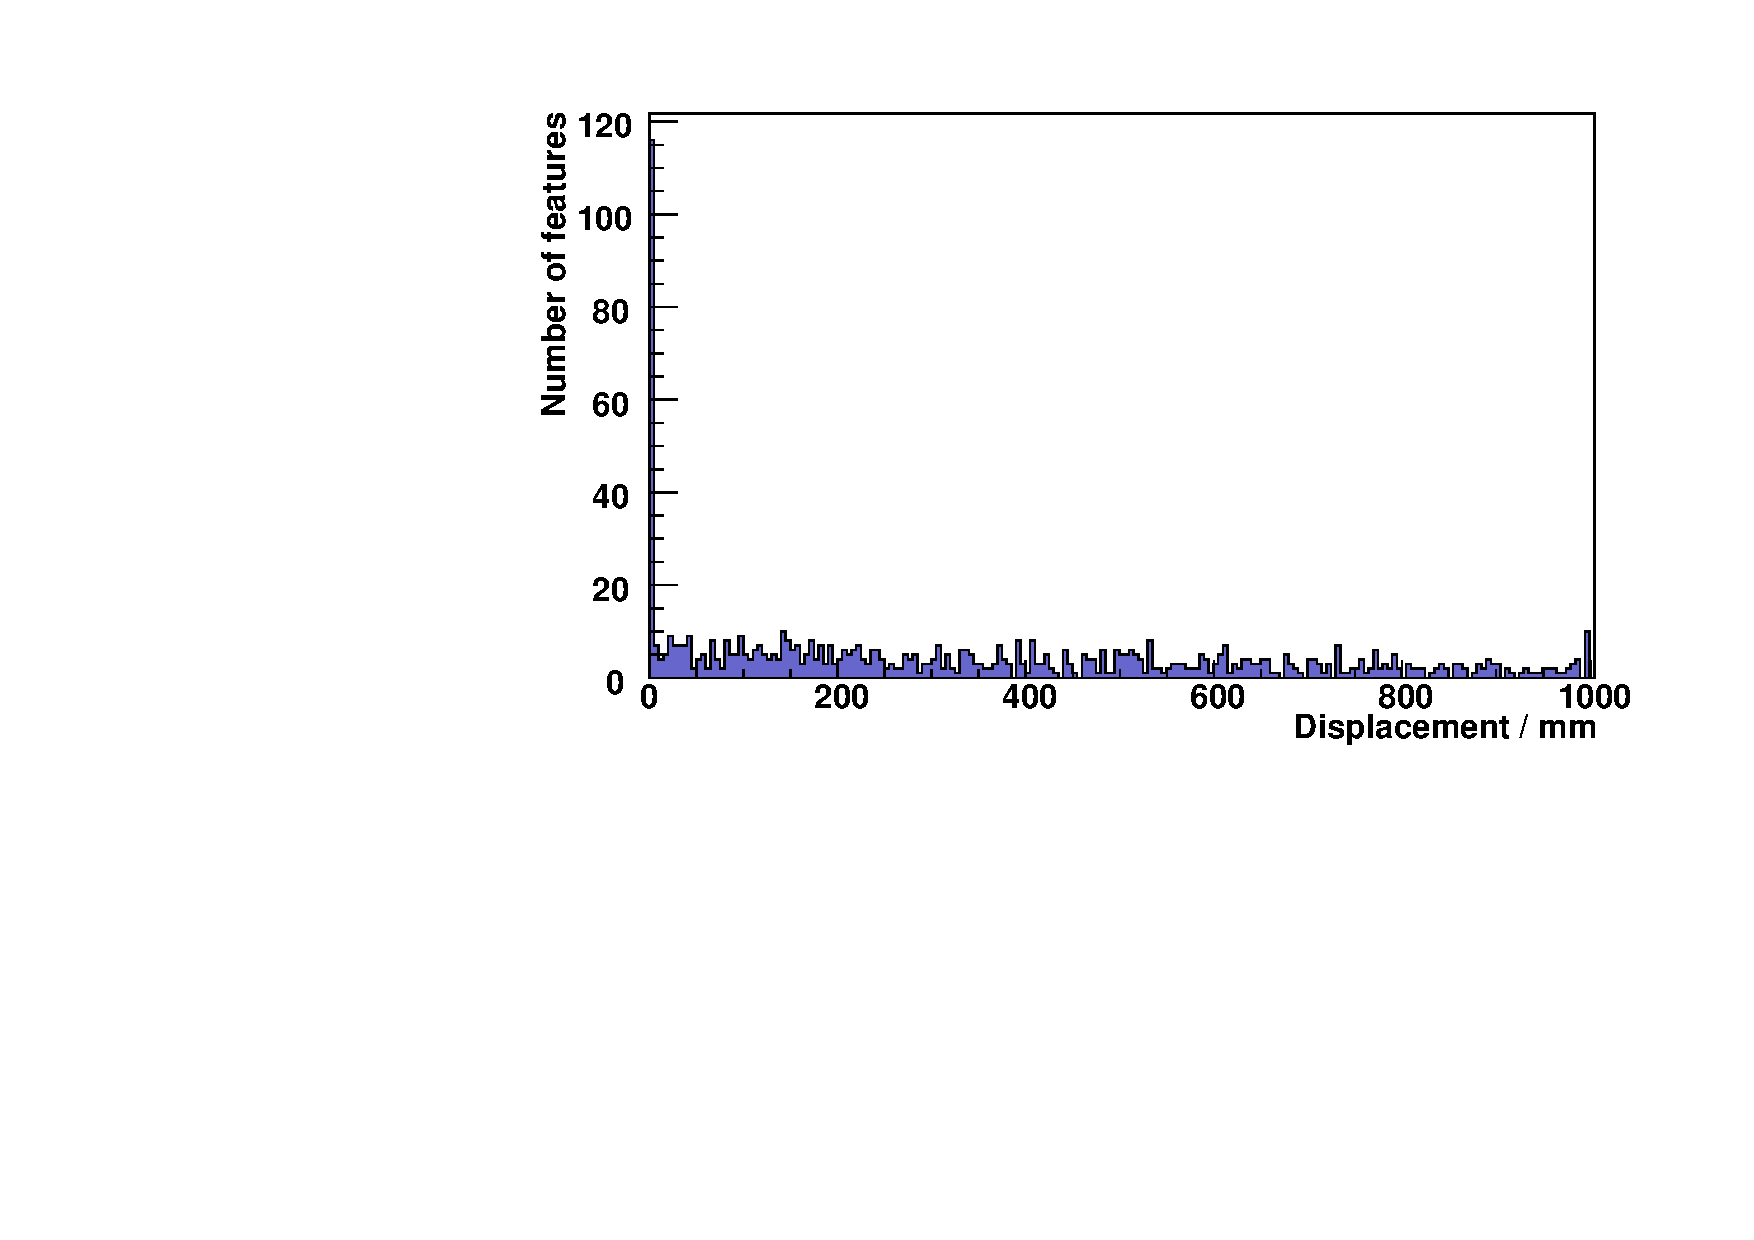
\includegraphics[width=0.35\textwidth,angle=-90]{chapters/latte_images/feature-displacement-qel}\label{fig:feature_3d_displacement}}
\subfigure[ ]{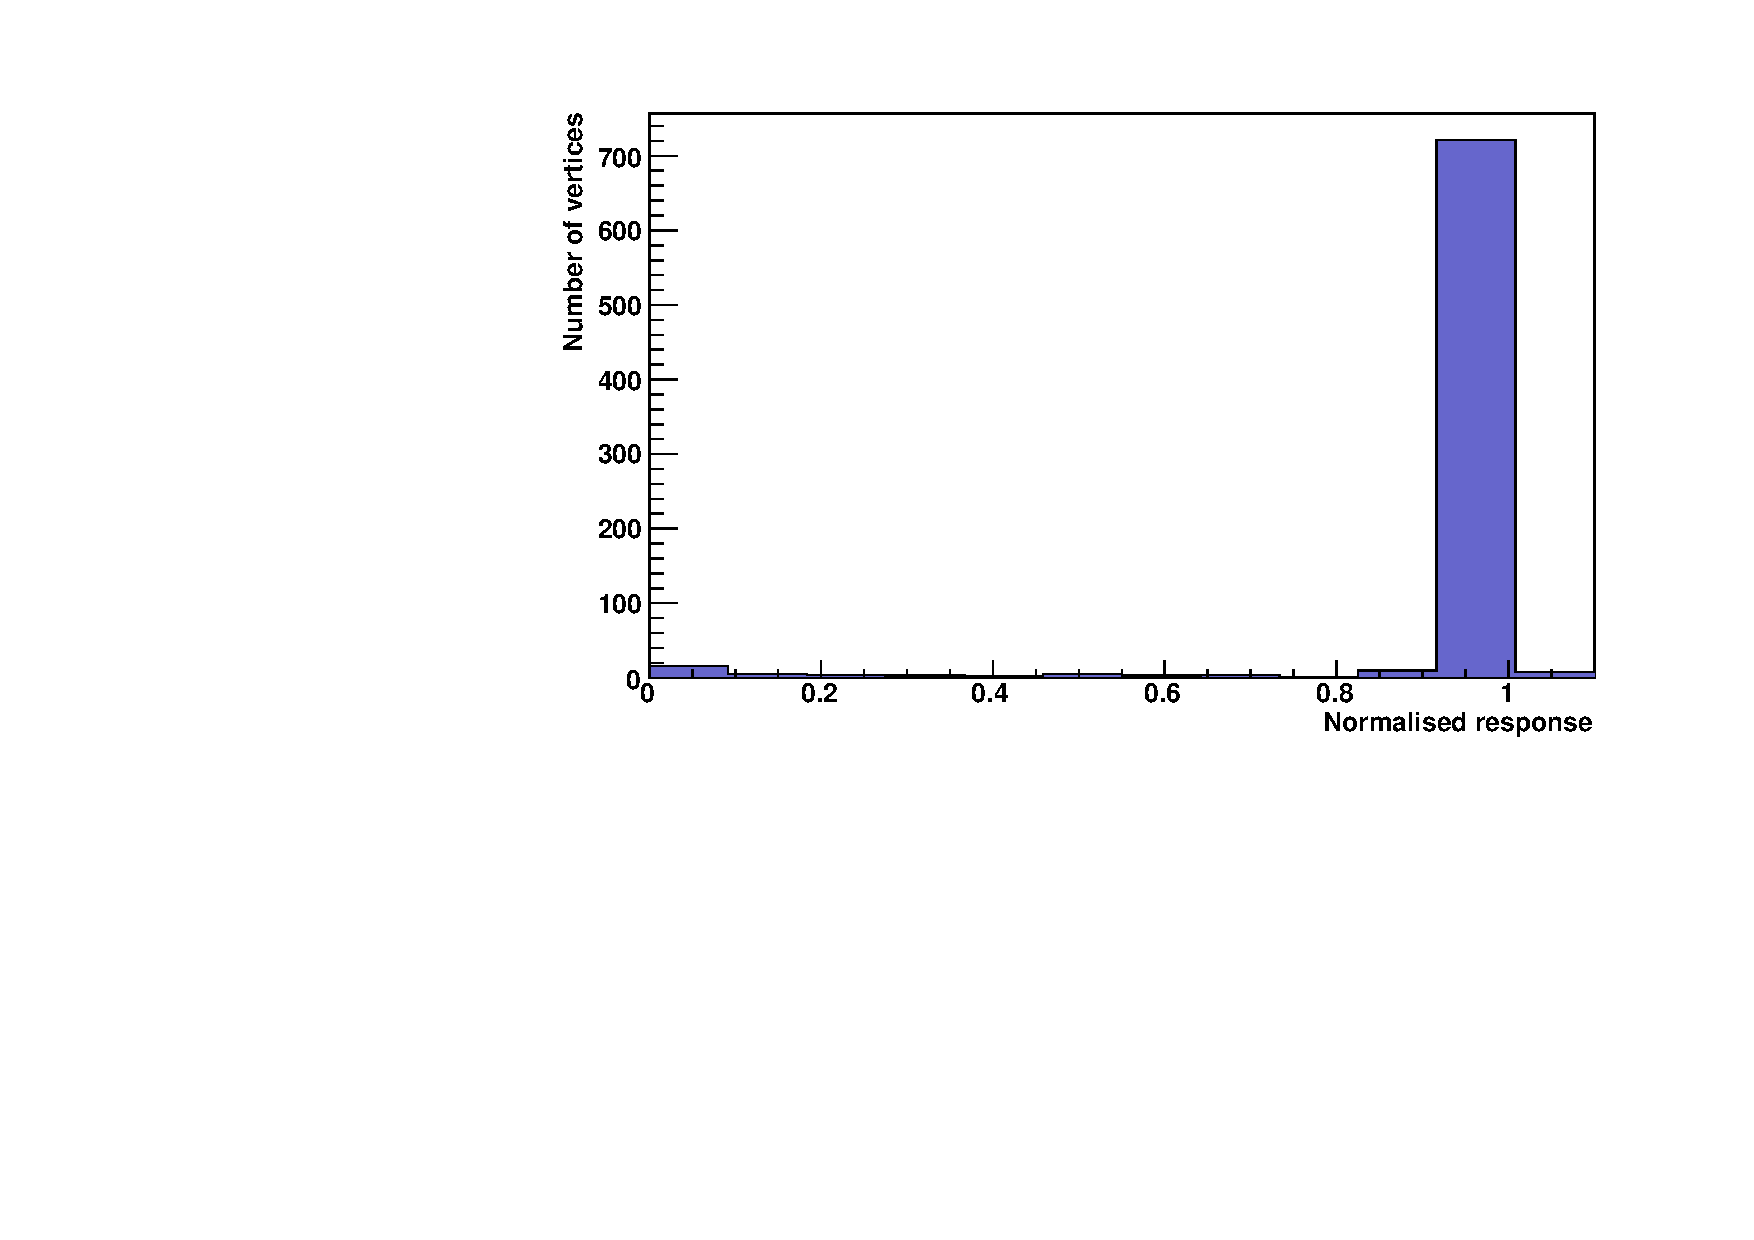
\includegraphics[width=0.35\textwidth,angle=-90]{chapters/latte_images/vertex-feature-response-qel}\label{fig:feature_3d_vertex_response}}
\caption[Performance of the feature detection service in 3D]{\label{fig:feature_3d}Performance of three-dimensional feature detection applied to \acs{CCQE} events. \subref{fig:feature_3d_counts} A small number of features are found in most events. \subref{fig:feature_3d_displacement} The distance between a feature found and the true event vertex is typically small (i.e. features are reasonably well located) but may be anywhere up to the radius of the detector, due to the noise introduced by delta electrons. \subref{fig:feature_3d_vertex_response} The vertex itself typically provides the strongest response of all features in the event.}
\end{figure}

\section{Feature Masking}
Latte provides a service to \emph{mask out} (remove) hits within a spherical region around a feature. The feature masking service presents a new view of the data, which does not include hits positioned less than some radius away from a central point. Each such point can be the location of a feature as determined by the feature detection algorithms of section \ref{sec:latte_feature_detection}, or in a special case the point $(0,0,0)$, referred to as \emph{origin masking}.

This service is useful because it allows algorithms to run on modified views of the event data, which often produces better results. One example would be in a clustering algorithm such as DBSCAN (see \ref{sec:latte_dbscan}), where the local point density affects the clustering. In this case, introducing a gap which corresponds to a feature such as a vertex results in a better clustering of tracks.

\section{Track Merging}\label{sec:cellularautomaton_merging}
Merging is performed using a cylindrical track road algorithm. Track candidates containing more than 100 hits are treated as key tracks for merging. A straight line in 3D is computed for each key track by the procedure below:

\begin{itemize}
	\item Determine a unit vector along the line of the track by using principal components analysis and choosing the component with the largest eigenvalue. This becomes the vector $\vec{n}$ along the line of the track.
	\item Determine a point on the line by computing the centroid coordinate of the hits corresponding to the track. This becomes the vector $\vec{p}$.
\end{itemize}

Each track is then represented by an infinite line in 3D, defined by equation \ref{eq:ca_track_3d_line} where the parameter $\lambda$ is a scalar representing distance along the line from the point $\vec{p}$ at which the point $\vec{l}$ is found.
\begin{equation}\label{eq:ca_track_3d_line}
\vec{l} = \vec{p} + \lambda \vec{n}
\end{equation}

The key tracks are iterated over, beginning with the longest, and hits from other (non-key) tracks are considered for merging into the key track if the distance $d$ from the hit to the line corresponding to the key track is less than some radius $r$. This defines a cylinder of radius $r$ around the key track, inside which any hits from other tracks are merged into the key track. The cylinder extends indefinitely either end of the key track; in practice this is not a problem due to the sparse nature of events resulting from neutrino interactions. Figure \ref{fig:ca_merging_cylinder} illustrates this merging process at a point where a track has been split into two pieces and a third cluster has been identified in the area.

\begin{figure}
\centering
\subfigure[Unmerged tracks]{\label{fig:ca_merging_initial}
	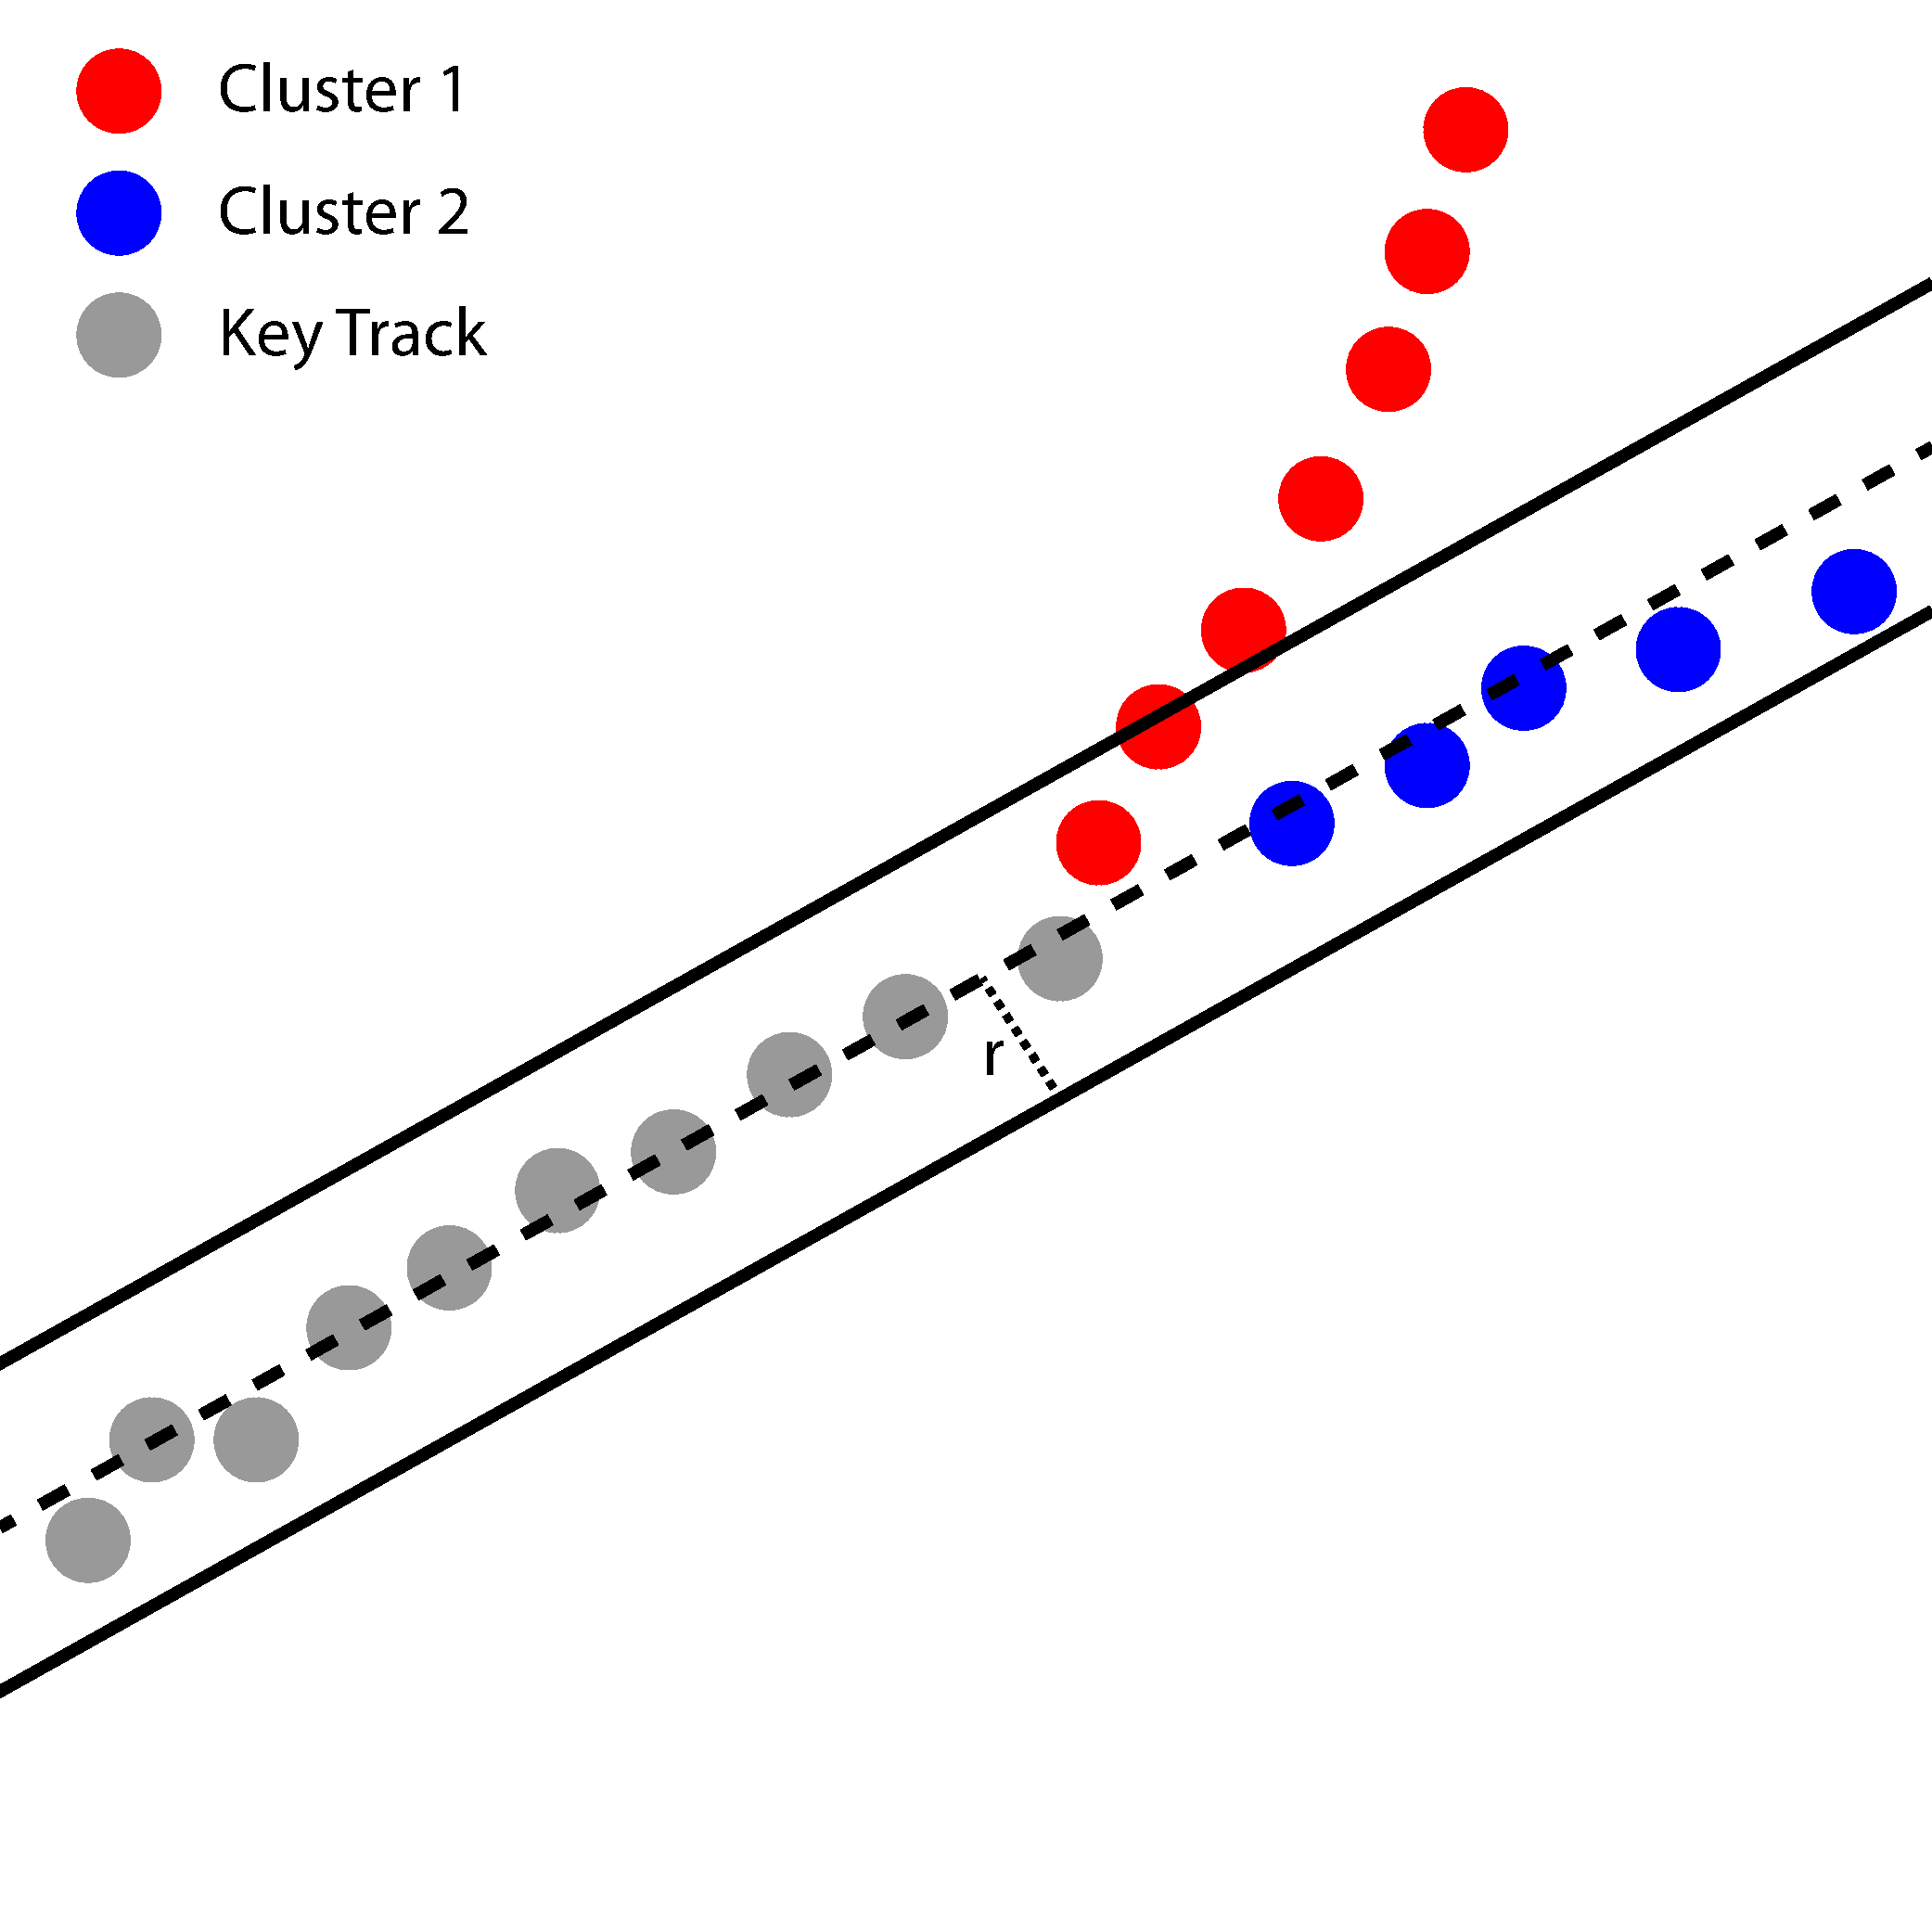
\includegraphics[width=0.35\textwidth]{chapters/cellularautomaton_images/Merging1}
}
\subfigure[Merged tracks]{\label{fig:ca_merging_final}
	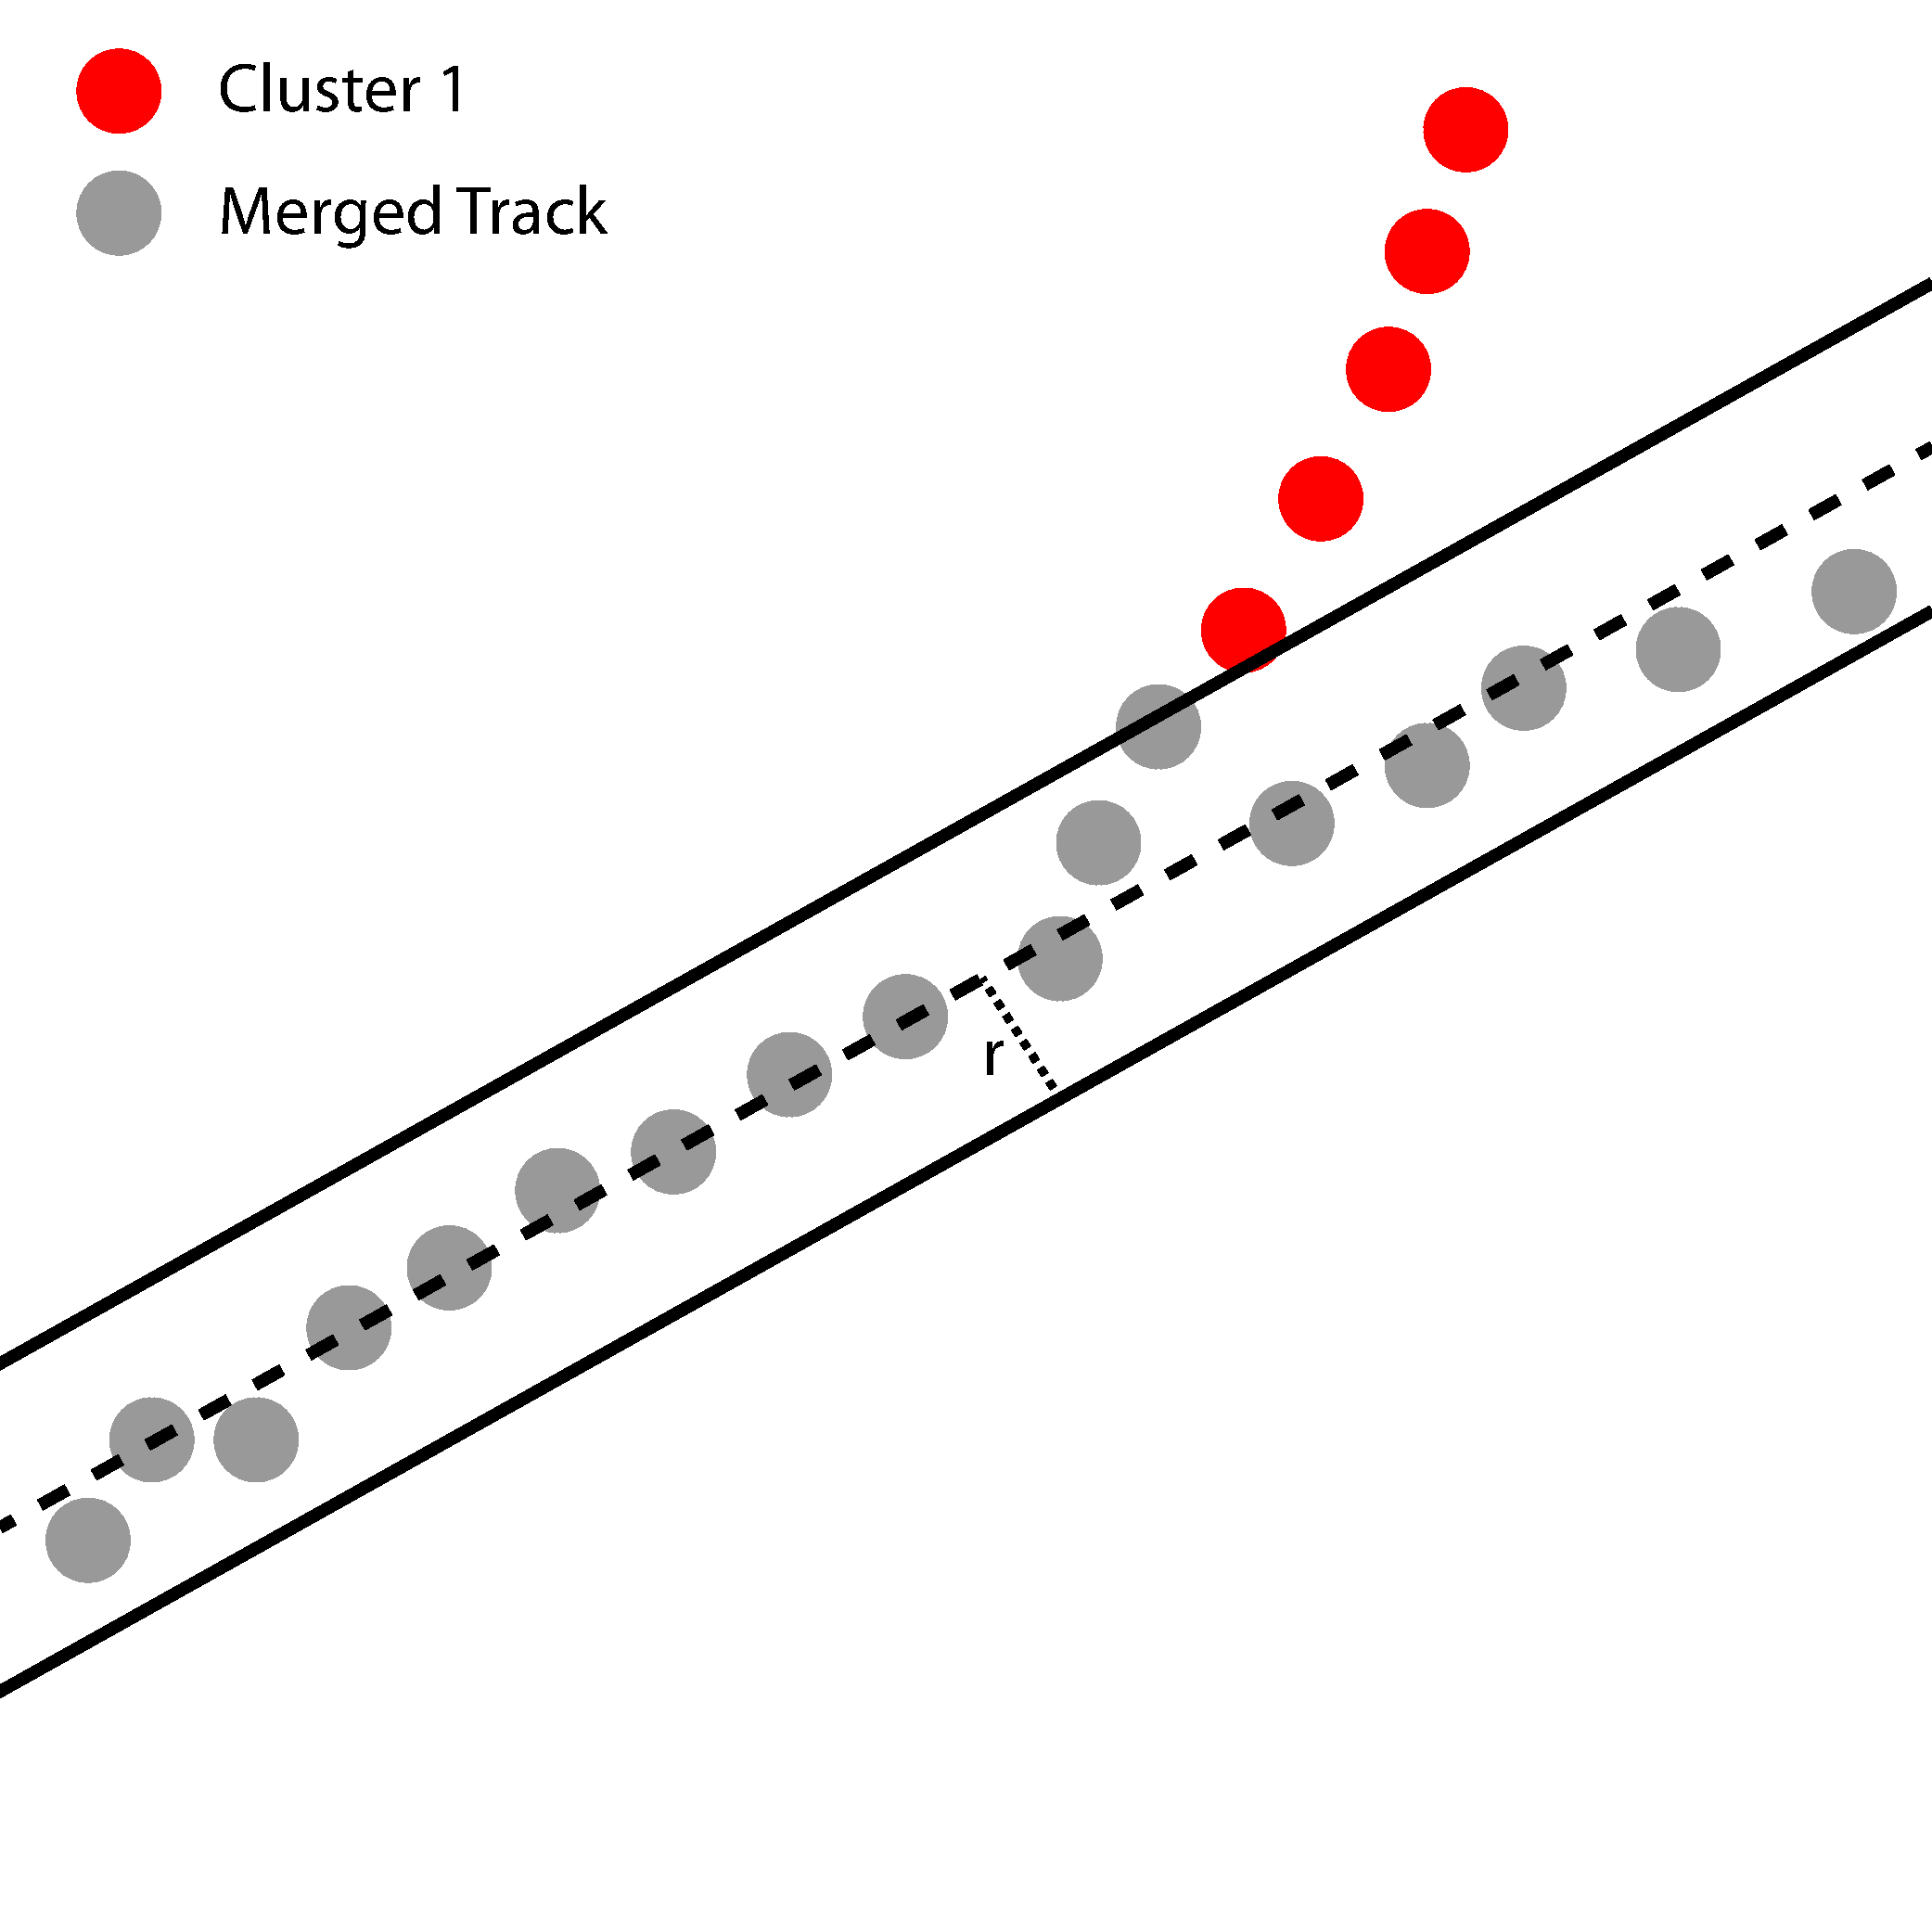
\includegraphics[width=0.35\textwidth]{chapters/cellularautomaton_images/Merging2}
}
\caption[Track road merging algorithm operating on clustered hits]{\label{fig:ca_merging_cylinder}The track road cylinder merging algorithm operating on the output of the \ac{CA}. \subref{fig:ca_merging_initial} shows the initial state with a key track and two smaller clusters. The cylinder drawn around the key track encloses all of cluster 2, but only two hits from cluster 1. \subref{fig:ca_merging_final} shows the resulting merged tracks; hits within the cylinder have been merged such that cluster 2 disappears altogether. Cluster 1 remains but has fewer hits than before.}
\end{figure}

The distance from a hit to the line is defined by taking two points $\vec{x}_1, \vec{x}_2$ on the line (by picking two values of $\lambda$) and, with $\vec{x}_0$ as the coordinates of a hit, the distance is given by equation \ref{eq:ca_dist_hit_line} (see also figure \ref{fig:ca_perp_dist}).
\begin{equation}\label{eq:ca_dist_hit_line}
d = \frac{|(\vec{x}_2 - \vec{x}_1) \times (\vec{x}_1 - \vec{x}_0)|}{|\vec{x}_2 - \vec{x}_1|}
\end{equation}

Hits which are merged into a key track are removed from their original track. Tracks which become empty as a result of this procedure are discarded. This procedure may leave some very small track fragments, which can be cleaned up by applying a range cut requiring any final state track to have some minimum number of hits. Currently, this range cut is set at 20 hits, corresponding to a straight-line track approximately $20\mm$ long, or a minimum ionising particle with $4.2\MeV$ kinetic energy.\footnote{A minimum ionising particle deposits $2.1\MeV \cm^{-1}$ in liquid Argon\citep{Aprile2006}.}

\begin{figure}
\centering
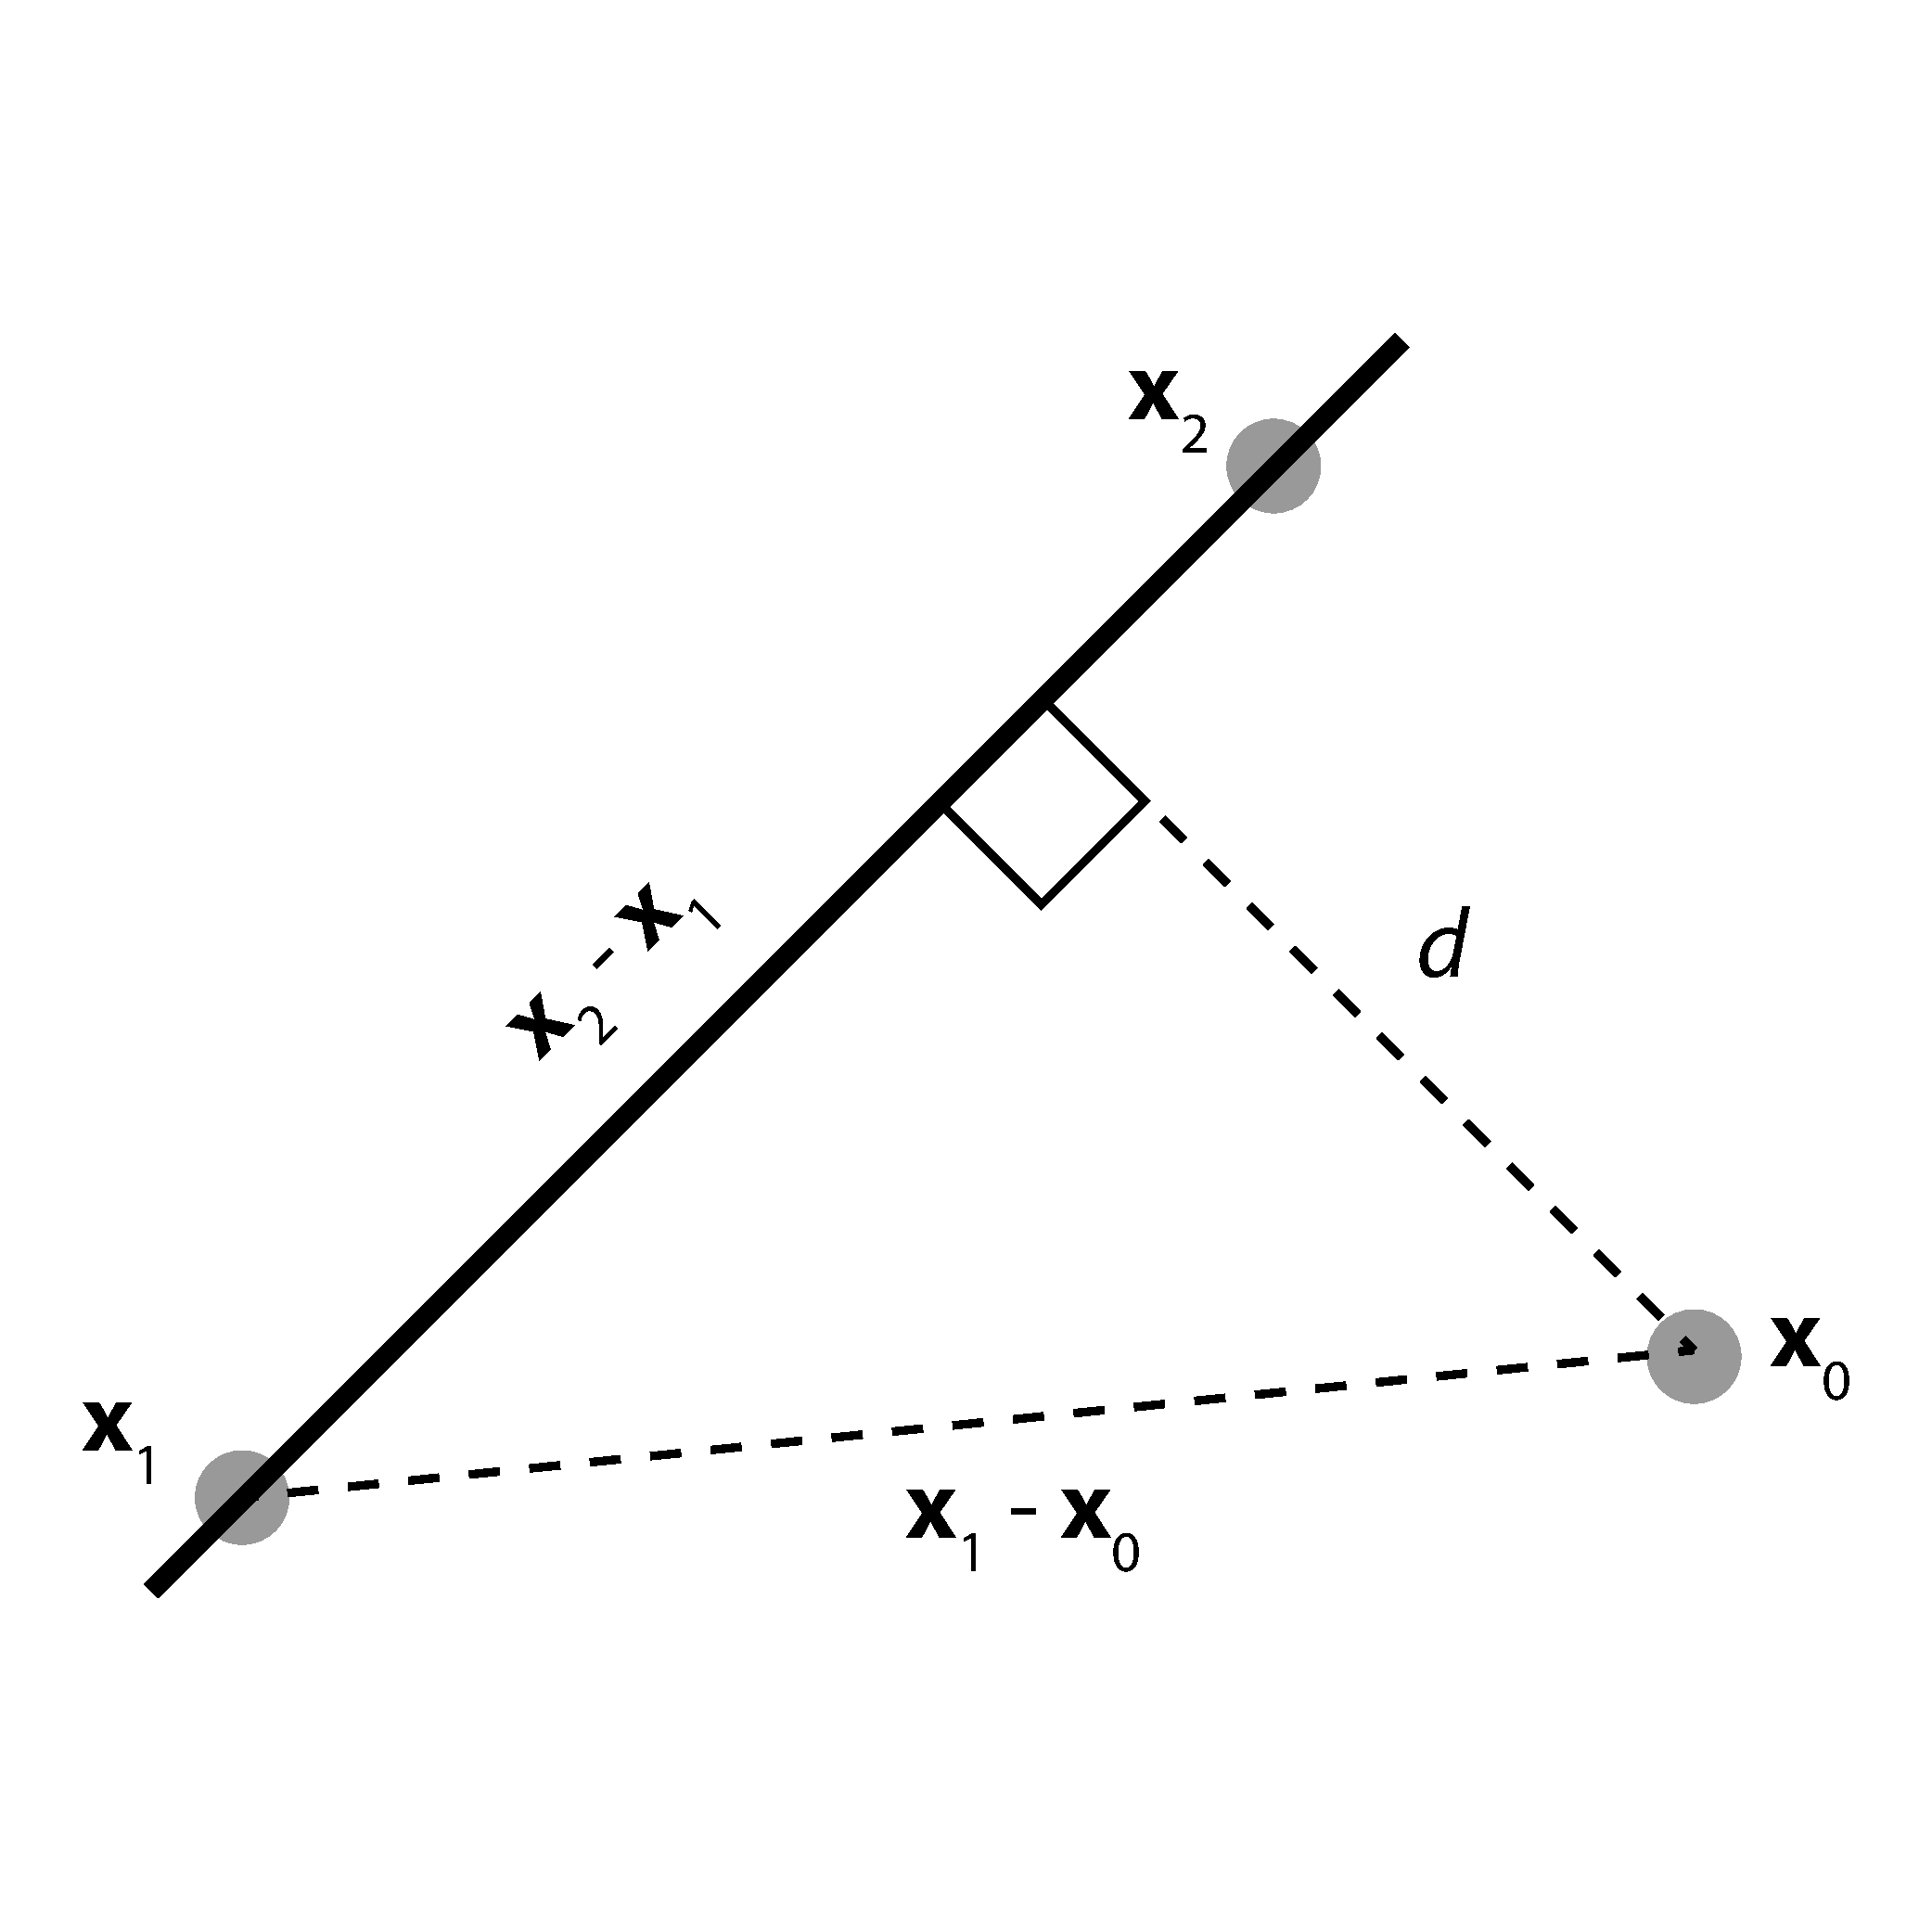
\includegraphics[width=0.5\textwidth]{chapters/cellularautomaton_images/PerpDist}
\caption[Perpendicular distance from a point to a line in 3D]{\label{fig:ca_perp_dist}Illustration of the perpendicular distance $d$ from the point $\vec{x}_0$ to the line between the points $\vec{x}_1$ and $\vec{x}_2$ according to equation \ref{eq:ca_dist_hit_line}.}
\end{figure}


\section{Truth Information}
When working with simulated events, it is often important to be able to access the \emph{truth information}, i.e. the information which was used to generate those events. The Latte framework provides two simulation packages. The first, \emph{PyTrackGen}, generates events consisting of one or more straight line tracks, and is designed to provide simplified representations of common event topologies. The second, \emph{Lamu}, provides a full Geant4 physics simulation, and can be seeded with events from the Genie event generator, or from manually constructed particle sources.

Both kinds of simulation write the truth information corresponding to lines or particles into their output formats, and the Latte framework provides a mechanism to access this information, query it for particle properties, and even make decisions based on it.

It is possible, for instance, to select only hits produced by electrons, or to obtain the true energy of the primary muon from a neutrino interaction. Such quantities are often compared against reconstructed quantities to provide a measure of the success of an algorithm.

\section{Range Cuts}
Latte provides a mechanism to filter event objects based on the number of hits they contain. For track-like objects, this corresponds approximately to the range of the particle. Range cuts can be applied based on the truth information (e.g. to select events where a proton track travelled more than some minimum reconstructible distance), or on reconstructed track objects (e.g. to cut out short track stubs, or to identify long tracks which may correspond to muons).

The range cuts are provided as either filters or wrappers. The filters allow for the selection of events based on track ranges recorded in truth information, while the wrappers present a reduced view of the event, in which the short tracks are not visible.

\section{Latte Control}
Latte Control is a mechanism for applying a sequence of algorithms to a set of events. In its simplest form, it allows the user to set up a \emph{pipeline} composed of service algorithms which are run in sequence on each event stored in a {\sc Root}\citep{Root} file.

\subsection{Event Objects}
A Latte \emph{Event} is essentially a Python dictionary\footnote{A set of key--value pairs. Some languages call them associative arrays, or maps.} with string keys mapped to arbitrary values. The \emph{LamuRun} file reader produces a single key called `raw', which maps to another dictionary containing keys for accessing the raw, simulated data. An \emph{Event object} in Latte Control is a fairly simple wrapper around this plain dictionary.

The wrapper exists primarily to abstract the idea of an event, so that the bulk of the Latte Control framework can deal with the abstract concept of an \emph{event-like object}. An event-like object is any Python object that provides all of the methods in the \texttt{latte.control.event.Event} class. This is useful because it allows us to wrap one event object inside another, thus modifying the behaviour of the event without having to change the original.

The base class, \texttt{latte.control.event.Event}, has the following functionality:
\begin{itemize}
\item A constructor, used internally by event loops (see chapter \ref{sec:latte-event-loops}). This is not usually called by a user of the framework.
\item \texttt{getFilename()}, which retrieves the file from which the event was read.
\item \texttt{getEventID()}, which returns the integer ID of the event within a file.
\item \texttt{getCurrentHitSelection()}, which returns a list of hits.
\item \texttt{getCurrentTracks()}, which returns a list of clusters (tracks).
\item \texttt{getKeys()}, which returns a list of keys defined in the event dictionary.
\item \texttt{hasKey(key)}, which returns \texttt{True} if the key exists, \texttt{False} otherwise.
\item \texttt{setKeyValue(key, value)}, which sets the key \texttt{key} to value \texttt{value}.
\item \texttt{addToKeyValue(key, value)}, which adds \texttt{value} to key \texttt{key}, creating it if it does not already exist.
\item \texttt{getKeyValue(key)}, which retrieves the value associated with the \texttt{key}.
\item \texttt{getUnderlyingEvent()}, which returns the event-like object that this object wraps (or \texttt{self} if it is the innermost layer).
\item \texttt{hasUnderlyingEvent()}, which returns \texttt{True} if this event object wraps another, \texttt{False} otherwise.
\end{itemize}

Most of the methods above allow for access to the keys and values of the dictionary itself. A wrapper class can modify these methods, and by doing so modify the details of how the dictionary is accessed. This allows for great flexibility in defining alternative views of events, for instance, where the set of hits presented differs from the set in the real event (e.g. by application of a range cut, or selection of hits from certain particle types).

In practice, the two most frequently altered methods are \texttt{getCurrentHitSelection()} and \texttt{getCurrentTracks()}. Most algorithms in Latte use these two methods to access the hits or clusters they will work on. In order to provide a modified set of hits or clusters, one simply needs to write an event wrapper to perform the necessary tasks. Event wrappers are discussed in the next section; this is the mechanism by which the range cuts and other modifying services in Latte work, without losing the original event data.

\subsection{Services \& Event Wrappers}
Algorithms made available in the Latte framework can be used with Latte Control in one of two ways. For general purpose reconstruction algorithms, Latte Control provides a corresponding \emph{Service}, which accepts an event object and performs some task. For example, the \emph{Merging} service provides an interface to the track merging algorithms provided in Latte and, when called, runs them on the active track selection. Services usually provide algorithms which are processor-intensive and add new information to the event, for example the allocation of hits to clusters, or the merging of multiple clusters based on certain criteria. Services typically augment an event object with the additional information they are able to provide.

In contrast, there are many cases where the goal of an algorithm is to present a different \emph{view} of the same data. One such example is the charge weighting algorithm, which shifts the position of each hit. Such algorithms are typically brought into the Latte Control framework as \emph{event wrappers}, which intercept attempts to access certain data that are already associated with an event, and present a modified version of that data. In this way, the original data is preserved, and can be retrieved by simply \emph{unwrapping} the event. Each event wrapper provides a \emph{wrapping service} which is used to apply the wrapper at an arbitrary point in the pipeline.

\subsection{Pipelines}
Each event is processed by a \emph{pipeline}, which is simply a sequence of service objects that are called in turn. Some services perform complex tasks such as clustering, while others wrap or unwrap an event, thus changing the views of data available for subsequent services. As events propagate through the pipeline, reconstructed information is added to them by the appropriate services, and may be written to disk (for example) at various points.

Since a Pipeline appears (to an outside observer) as just another callable object which accepts events, it is possible to put pipelines within pipelines, for example to group related services into logical \emph{tasks} (such as grouping clustering and merging of tracks into a \emph{tracking} task), or to provide decision making, using a service which chooses to execute one of several pipelines based on the value (or existence) of certain data in the event.

This flexibility means that the pipeline structure of Latte Control is capable of performing complicated analyses without needing further core support. A user can simply stick together the components they need, in the correct order, then leverage the power of Latte Control to run their analysis job over the available data.

\subsection{Event Loops}\label{sec:latte-event-loops}
At the highest level, Latte Control provides an event loop which is capable of reading a range of events from a {\sc Root} file and passing each event in turn through a pipeline of Latte Control services. In this manner, it is possible to easily write reconstruction scripts which configure a number of services, stick them together in an arbitrary order into a pipeline, and have that pipeline applied to each event in a file. This provides a powerful mechanism for writing physics analysis scripts which make use of the Latte-provided services as well as intermediate or final \emph{analysis} services, using the data available in an event to measure physically useful quantities. Since the objects representing pipeline segments persist between events, they can also be used to build up statistics over an entire set of events. When the event loop finishes, the analysis object can be queried for the set of statistical data it has collected.



%% --------------------------------------------------
%% CHAPTER: Cellular Automaton
%% --------------------------------------------------
\chapter{A Cellular Automaton for Track Reconstruction}\label{chapter:CellularAutomaton}

\section{Cellular Automata}
A \acf{CA} is a \ac{FSM} which usually consists of a regular grid of cells in a finite number of dimensions, each of which exists in one of a finite number of states. A neighbourhood is defined to be some region around any given cell, and the next generation is formed by updating the state of each cell according to a fixed rule which takes into account the current cell state as well as the state of its neighbours. Typically, this rule is identical for each cell and at each time step. The update rule is usually applied simultaneously to the whole grid.

The concept was originally devised by John von Neumann\citep{vonNeumann1966} in the 1940s as a method of creating self-reproducing machines using a \ac{CA} with 29 states. Cellular automata became popular in the 1970s with the development of the \emph{Game of Life} by John Conway (see, for example, \citep{Gardner1970}). In \emph{Life}, cells exist in one of two states (live or dead) and the neighbourhood is defined to be the 8 cells surrounding a central cell on a square grid. The update rules are simple but result in varied and complex behaviour. Figure \ref{fig:ca_life_four_steps} illustrates these rules for the first four states of a simple initial pattern.

\begin{enumerate}
\item Any live cell with $< 2$ live neighbours dies (under-population).
\item Any live cell with 2 or 3 live neighbours lives on.
\item Any live cell with $> 3$ live neighbours dies (over-population).
\item Any dead cell with exactly 2 live neighbours becomes live (reproduction).
\end{enumerate}

\begin{figure}
\centering
\subfigure[Step 1]{
	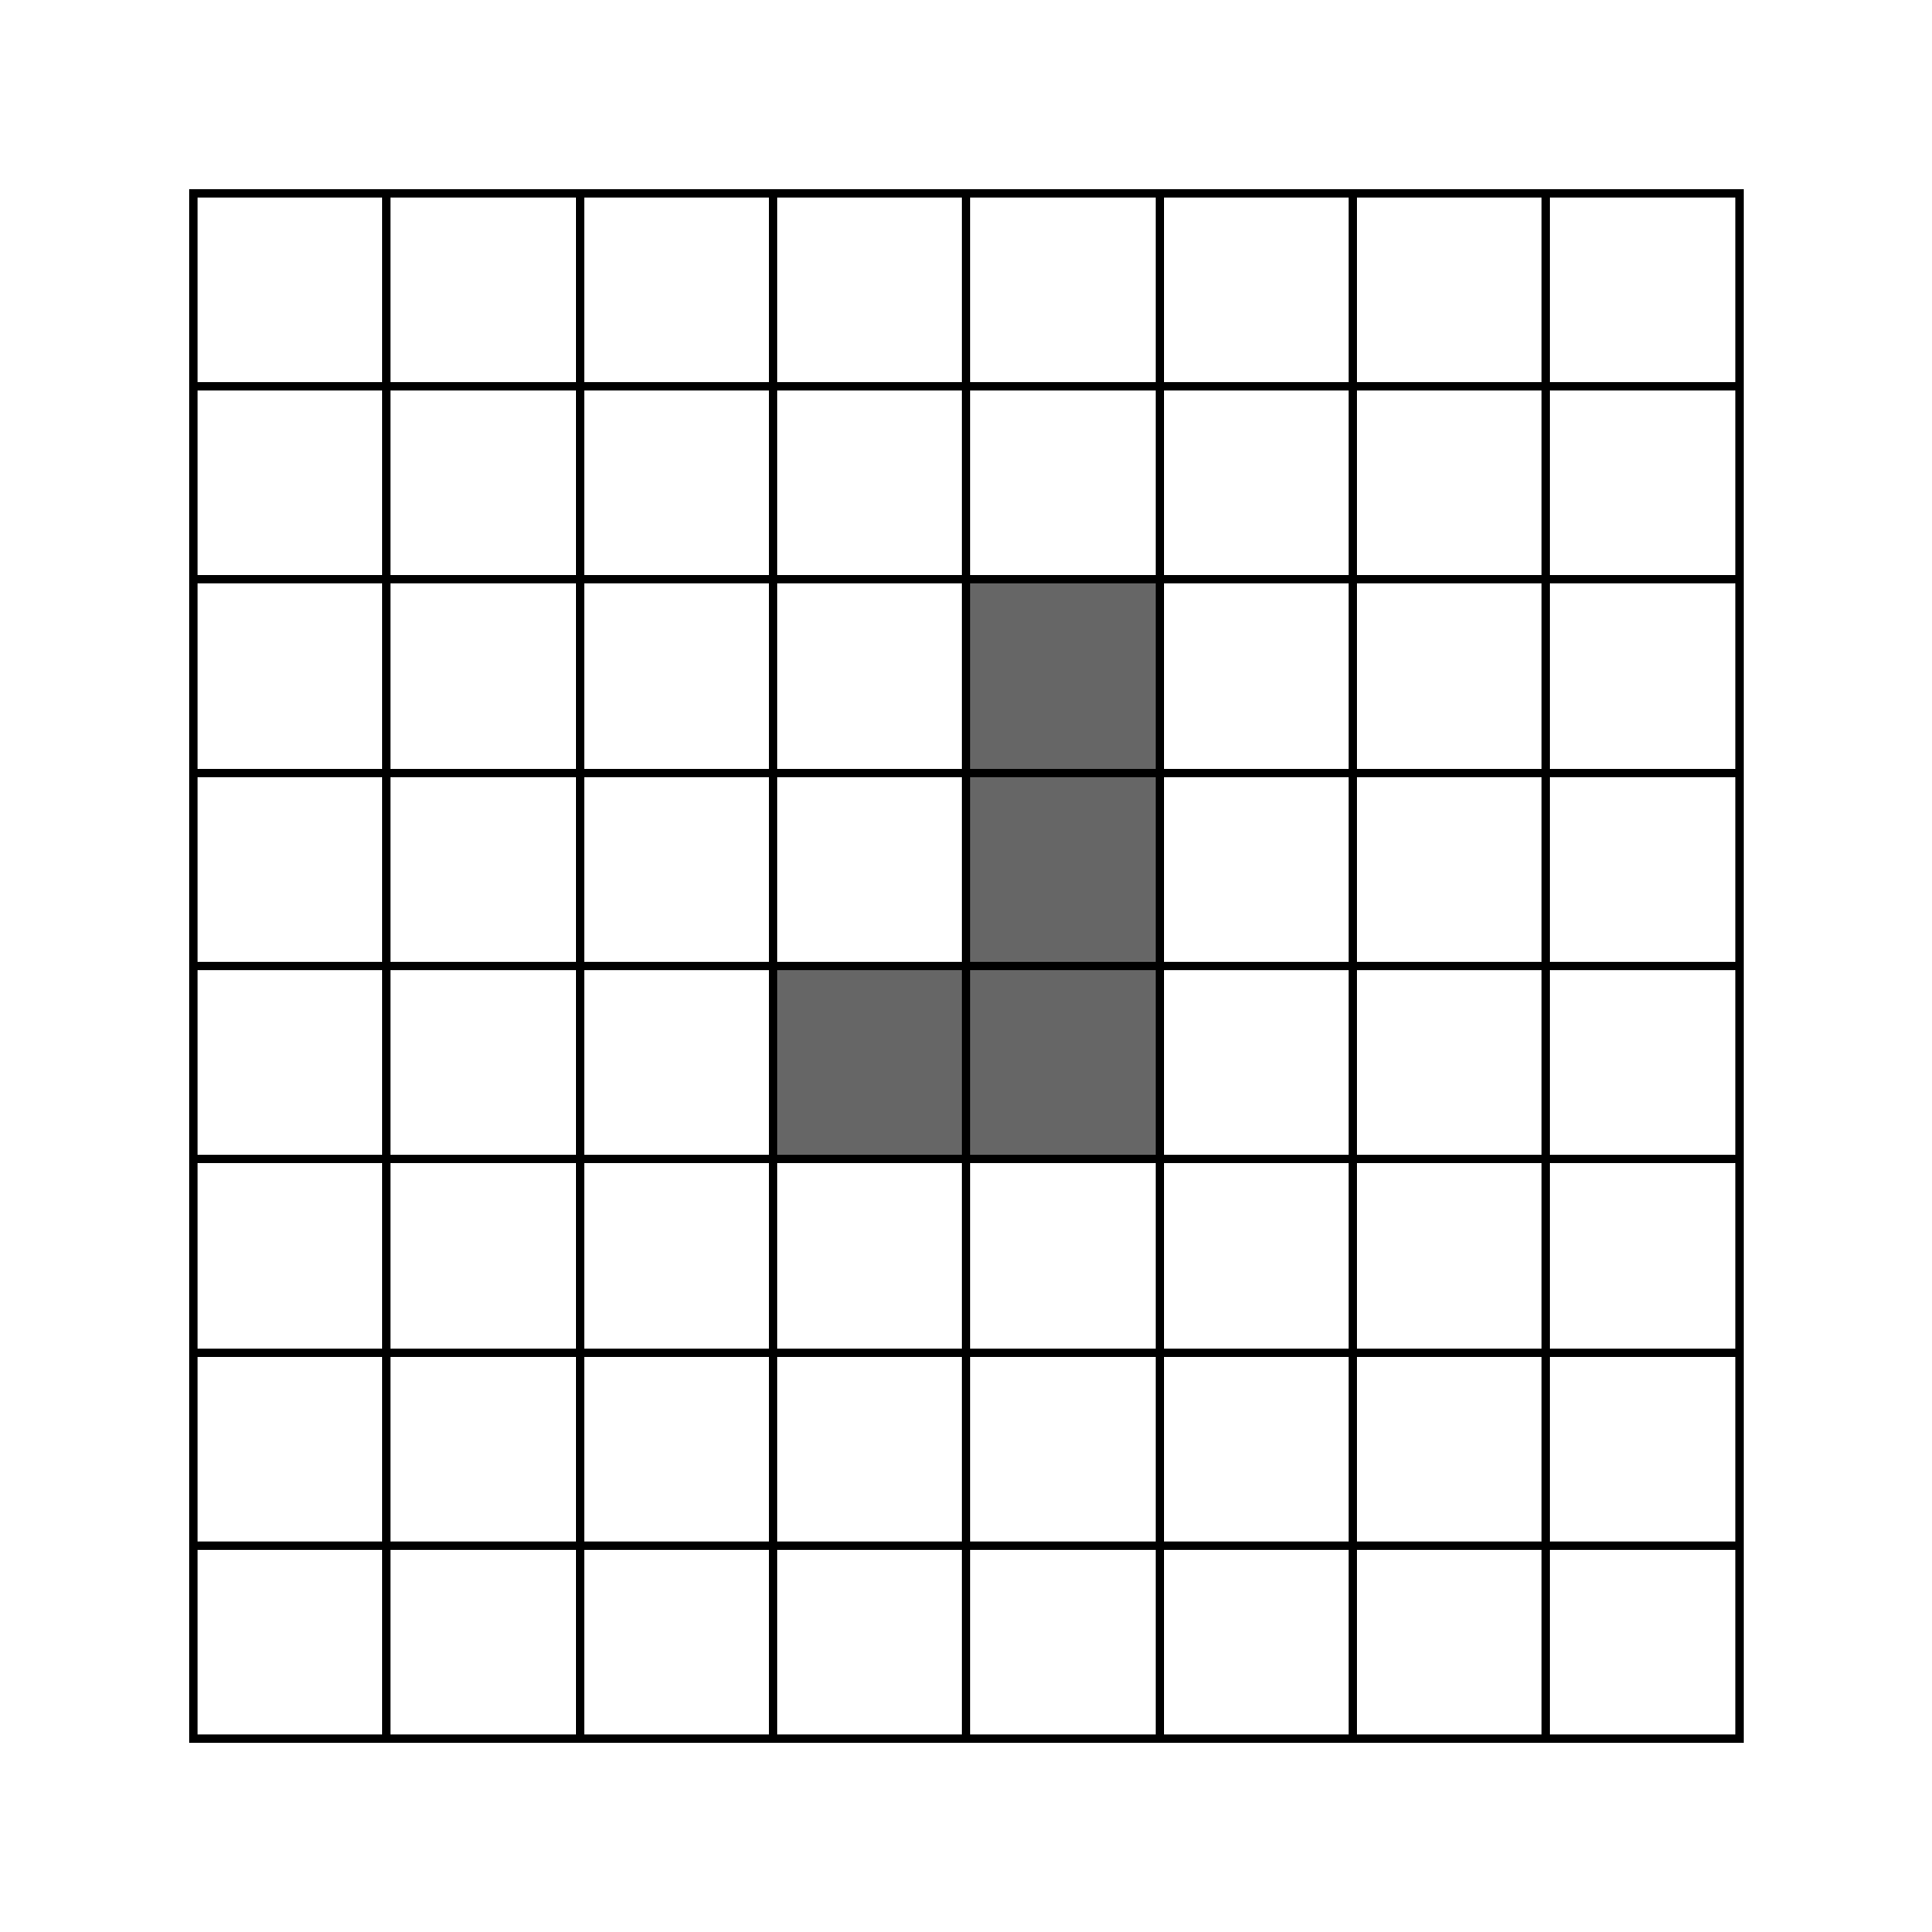
\includegraphics[width=0.2\textwidth]{chapters/cellularautomaton_images/Life1}
	\label{fig:ca_life_four_steps_step1}
}
\subfigure[Step 2]{
	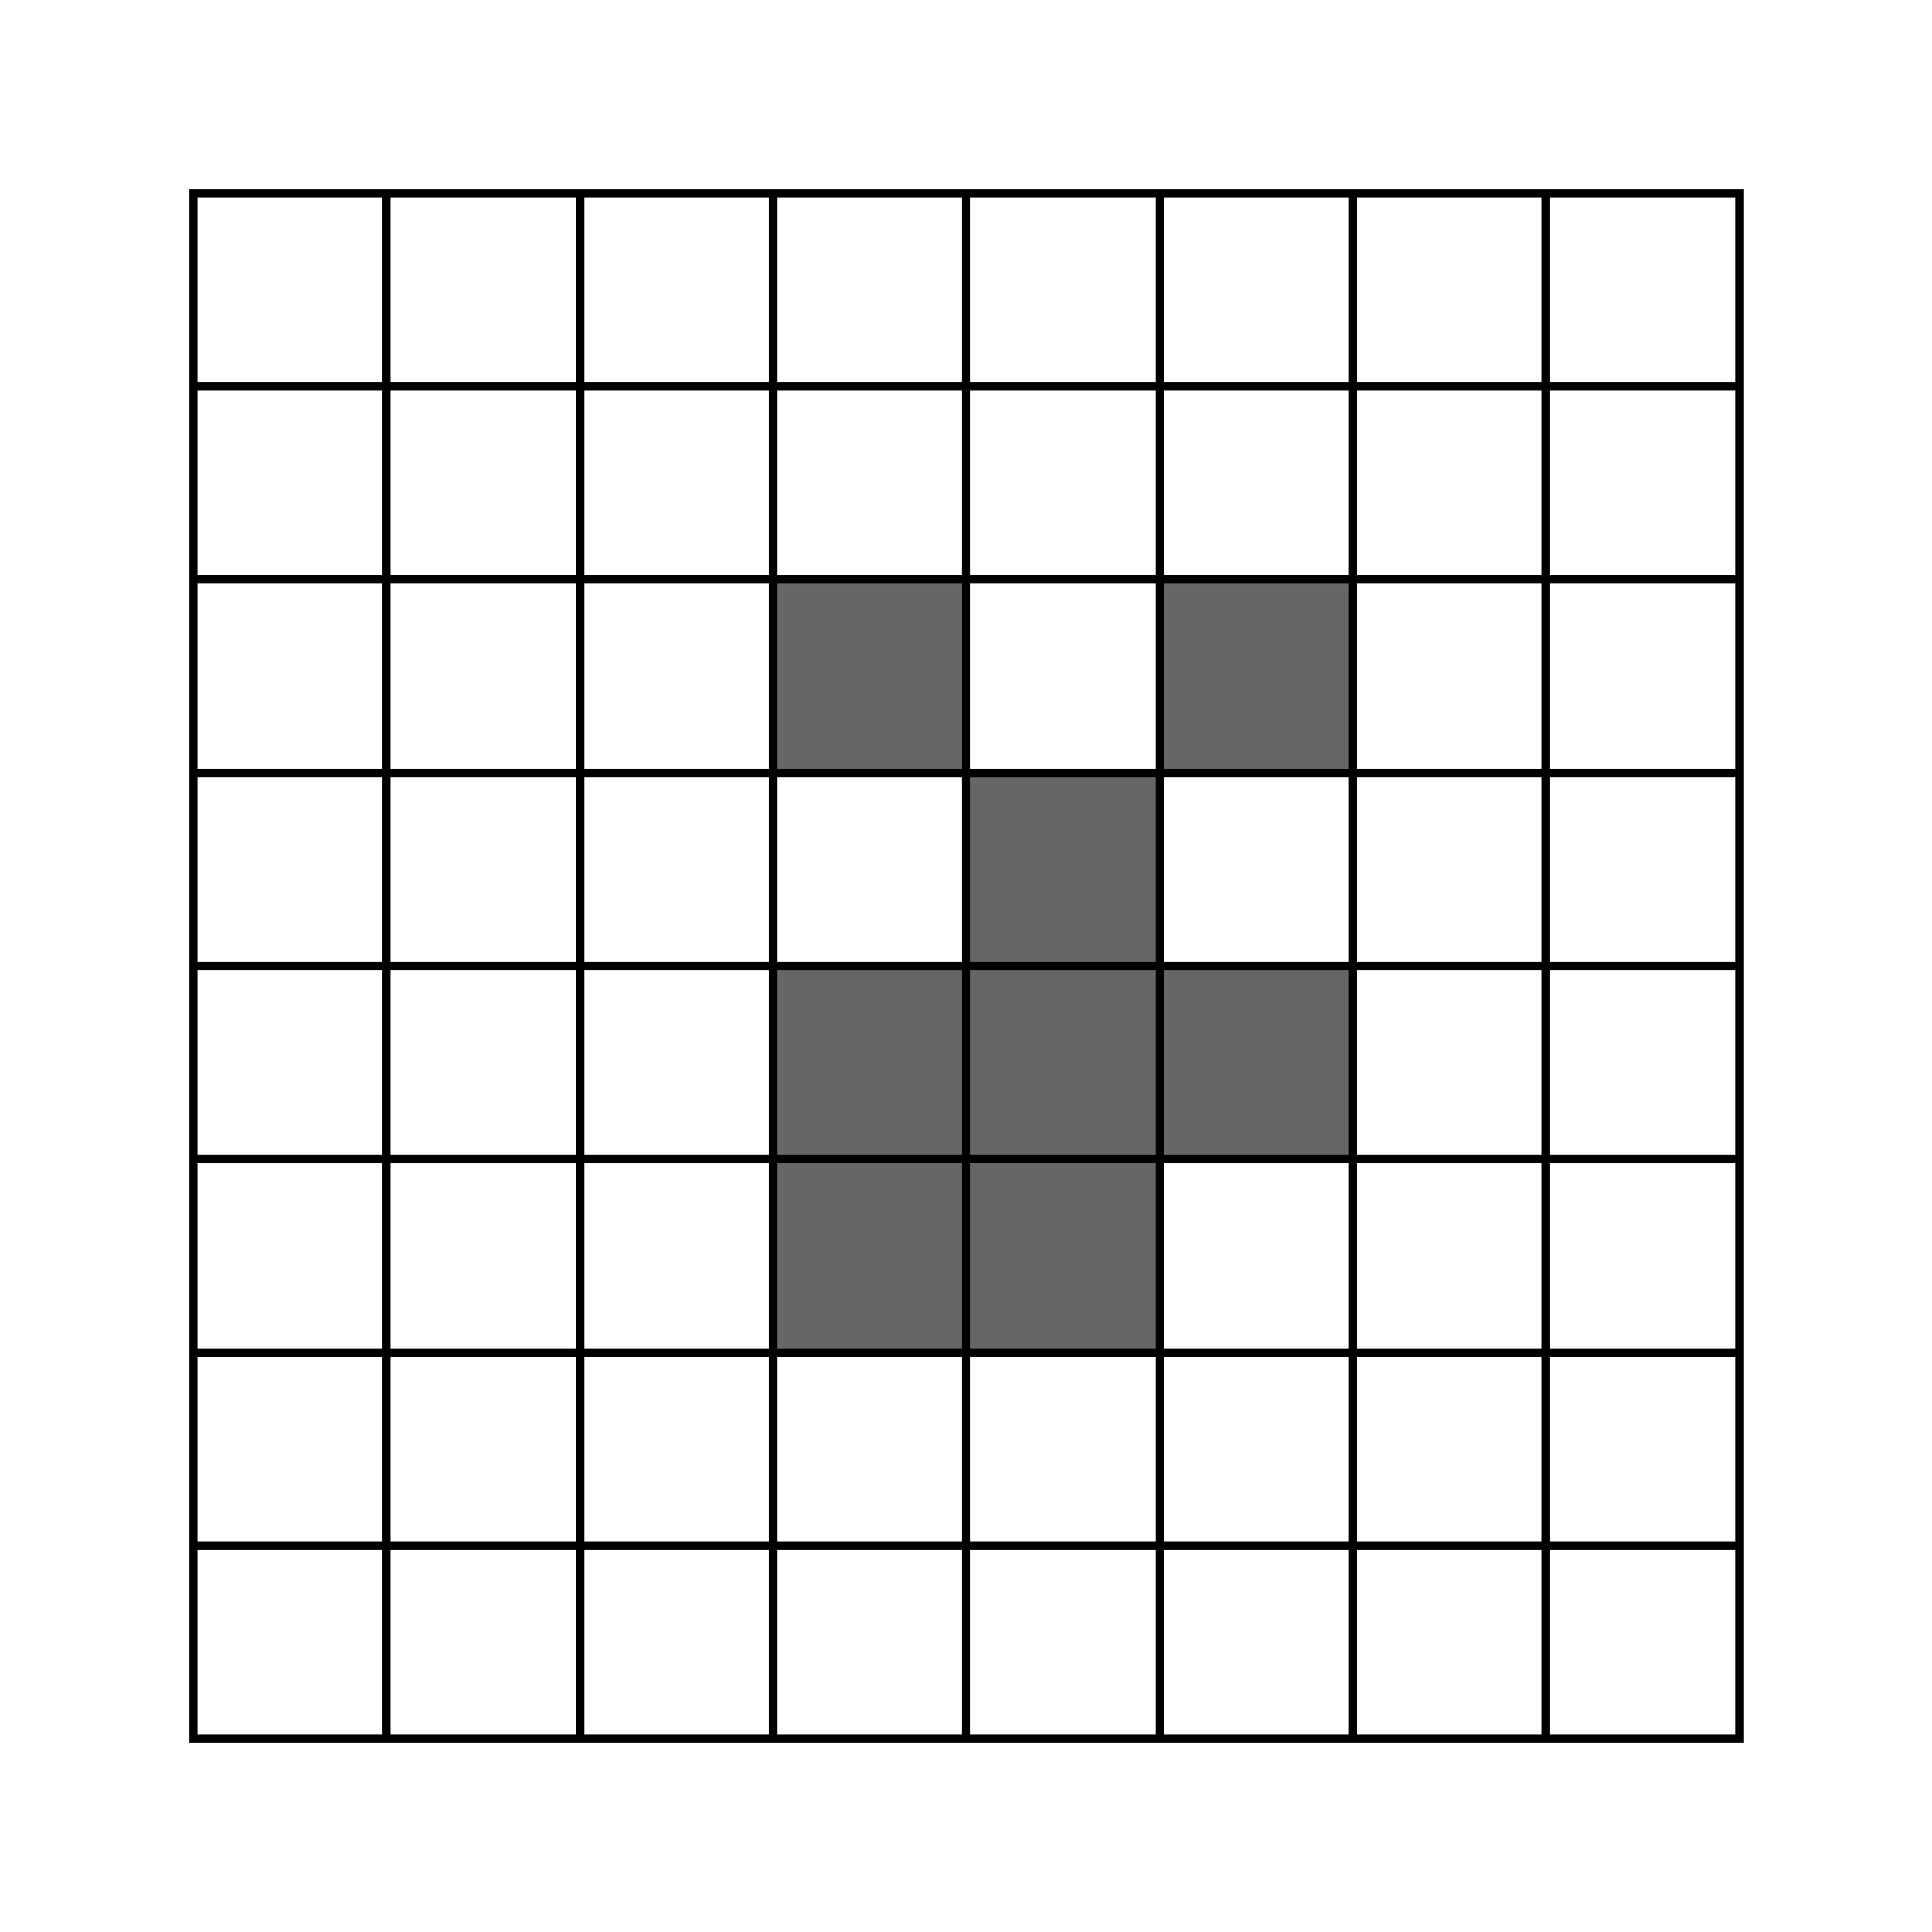
\includegraphics[width=0.2\textwidth]{chapters/cellularautomaton_images/Life2}
	\label{fig:ca_life_four_steps_step2}
}
\subfigure[Step 3]{
	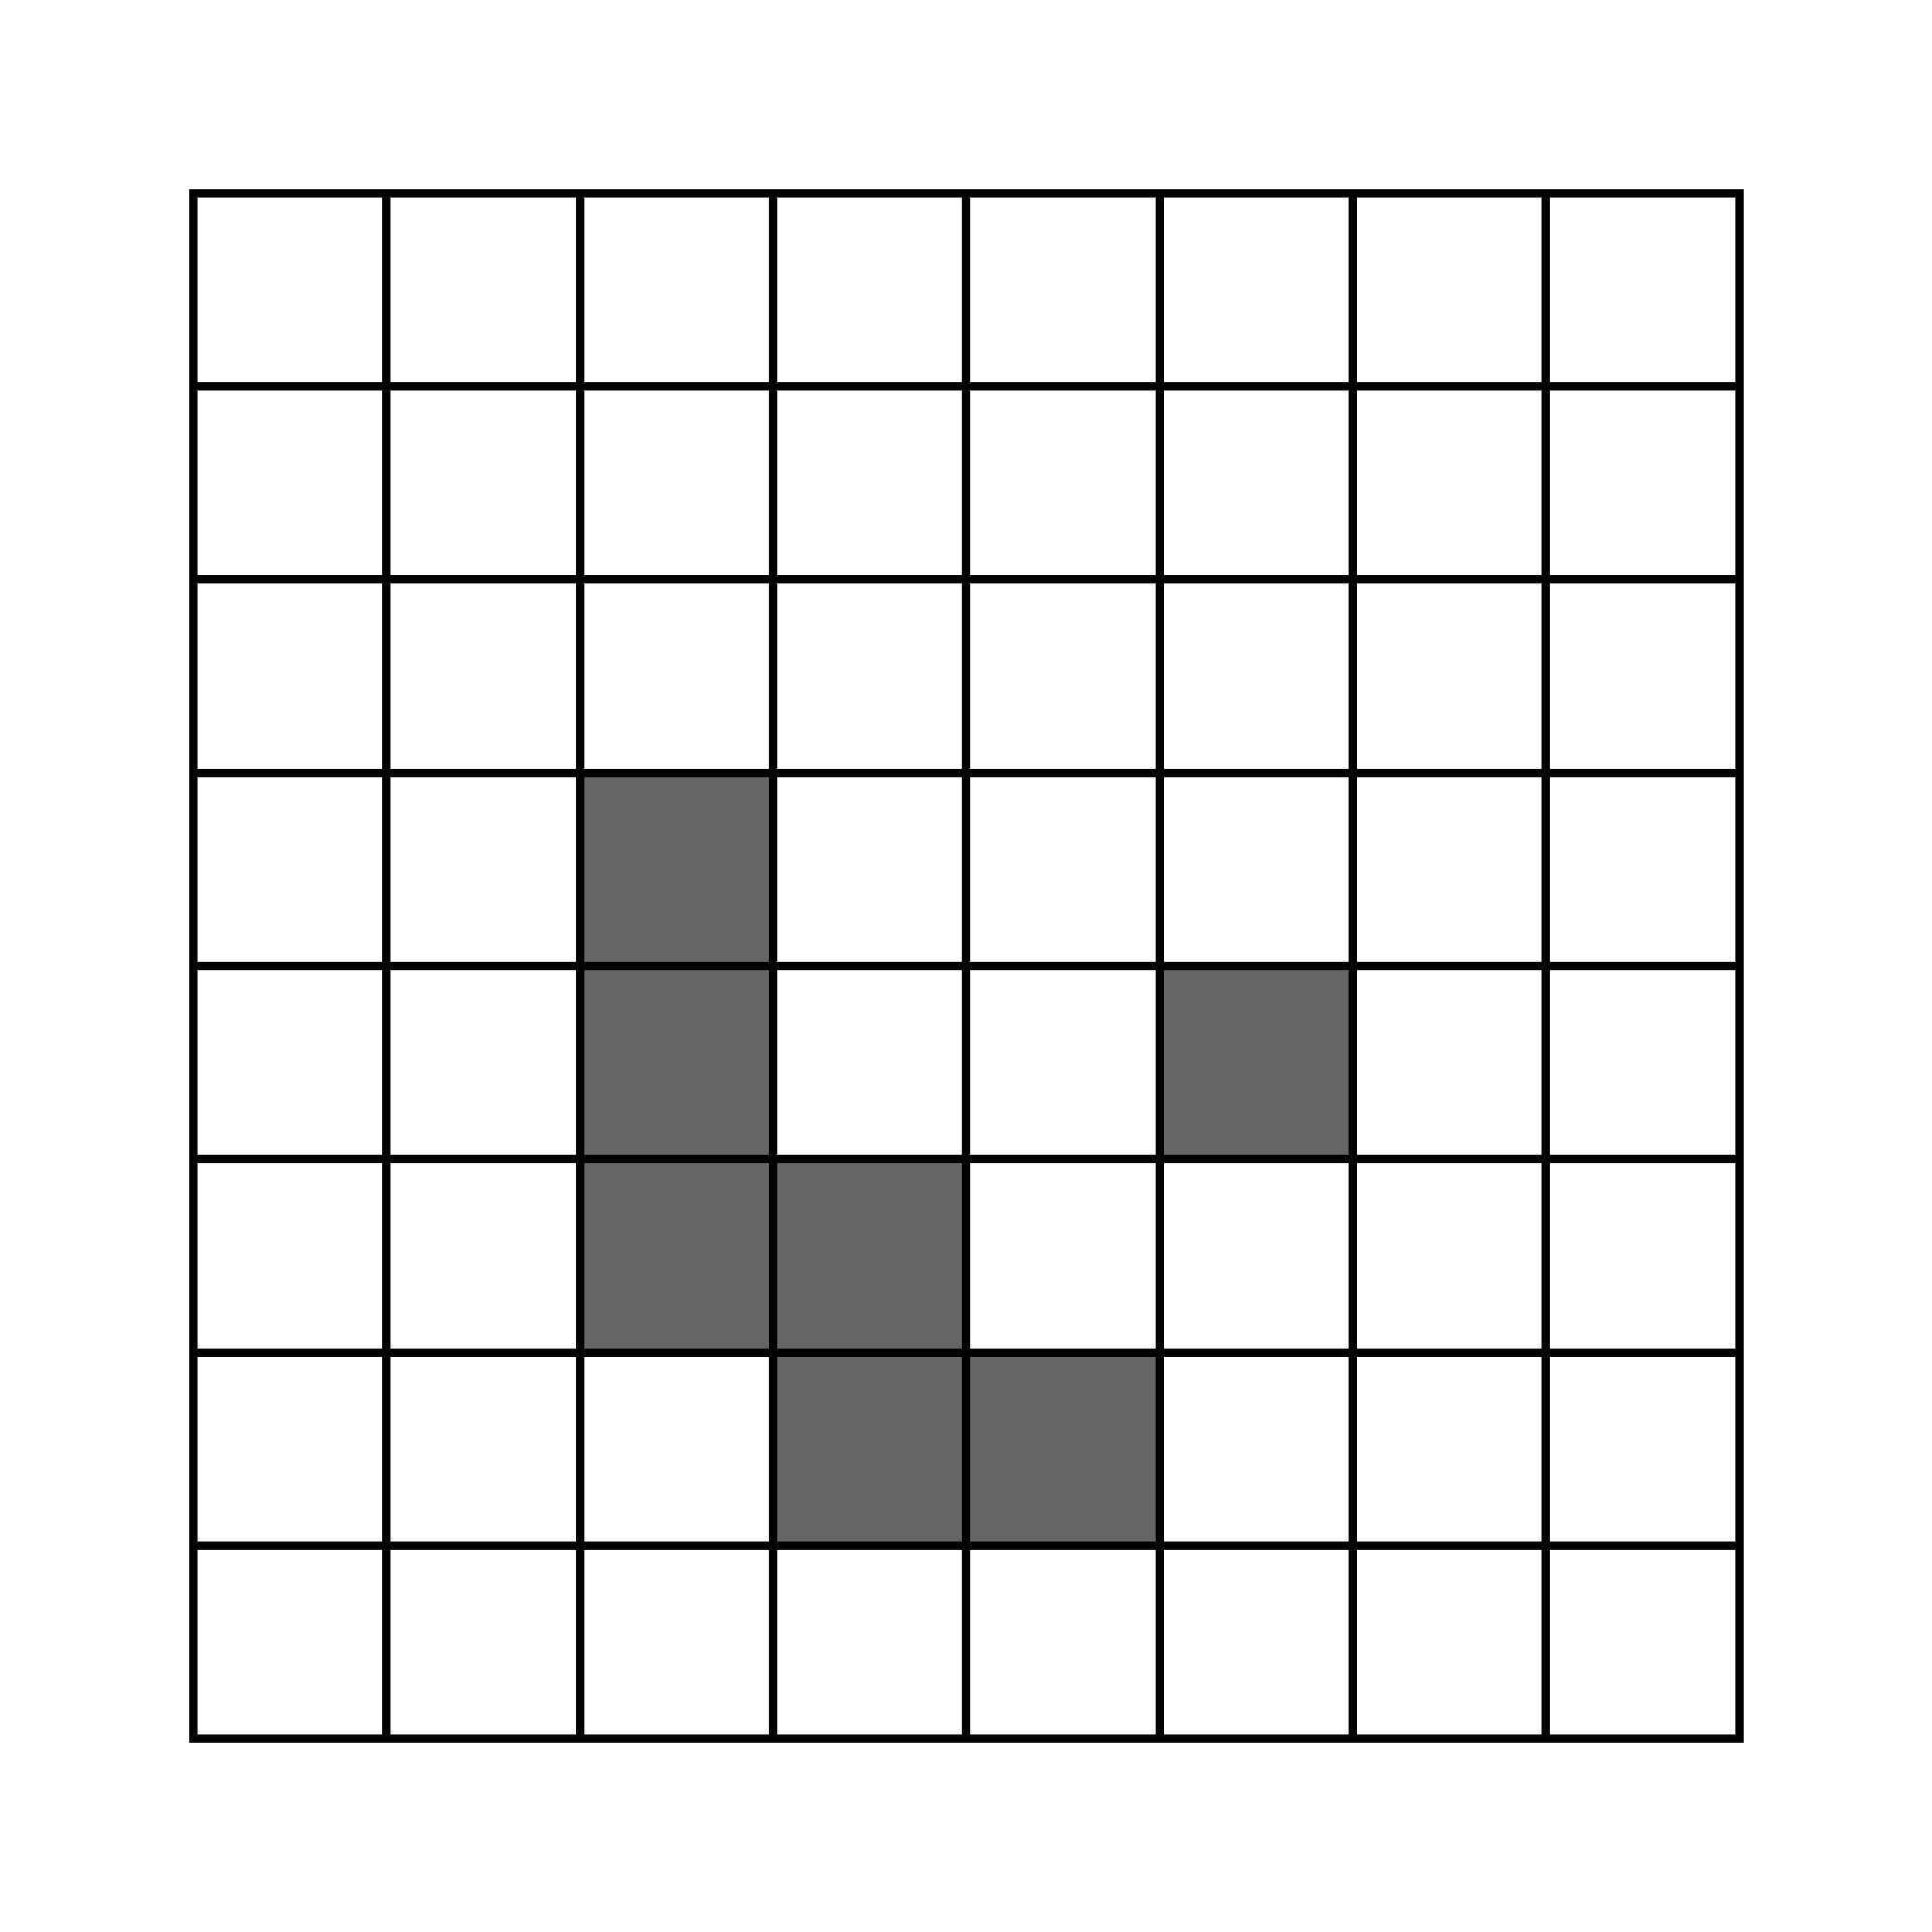
\includegraphics[width=0.2\textwidth]{chapters/cellularautomaton_images/Life3}
	\label{fig:ca_life_four_steps_step3}
}
\subfigure[Step 4]{
	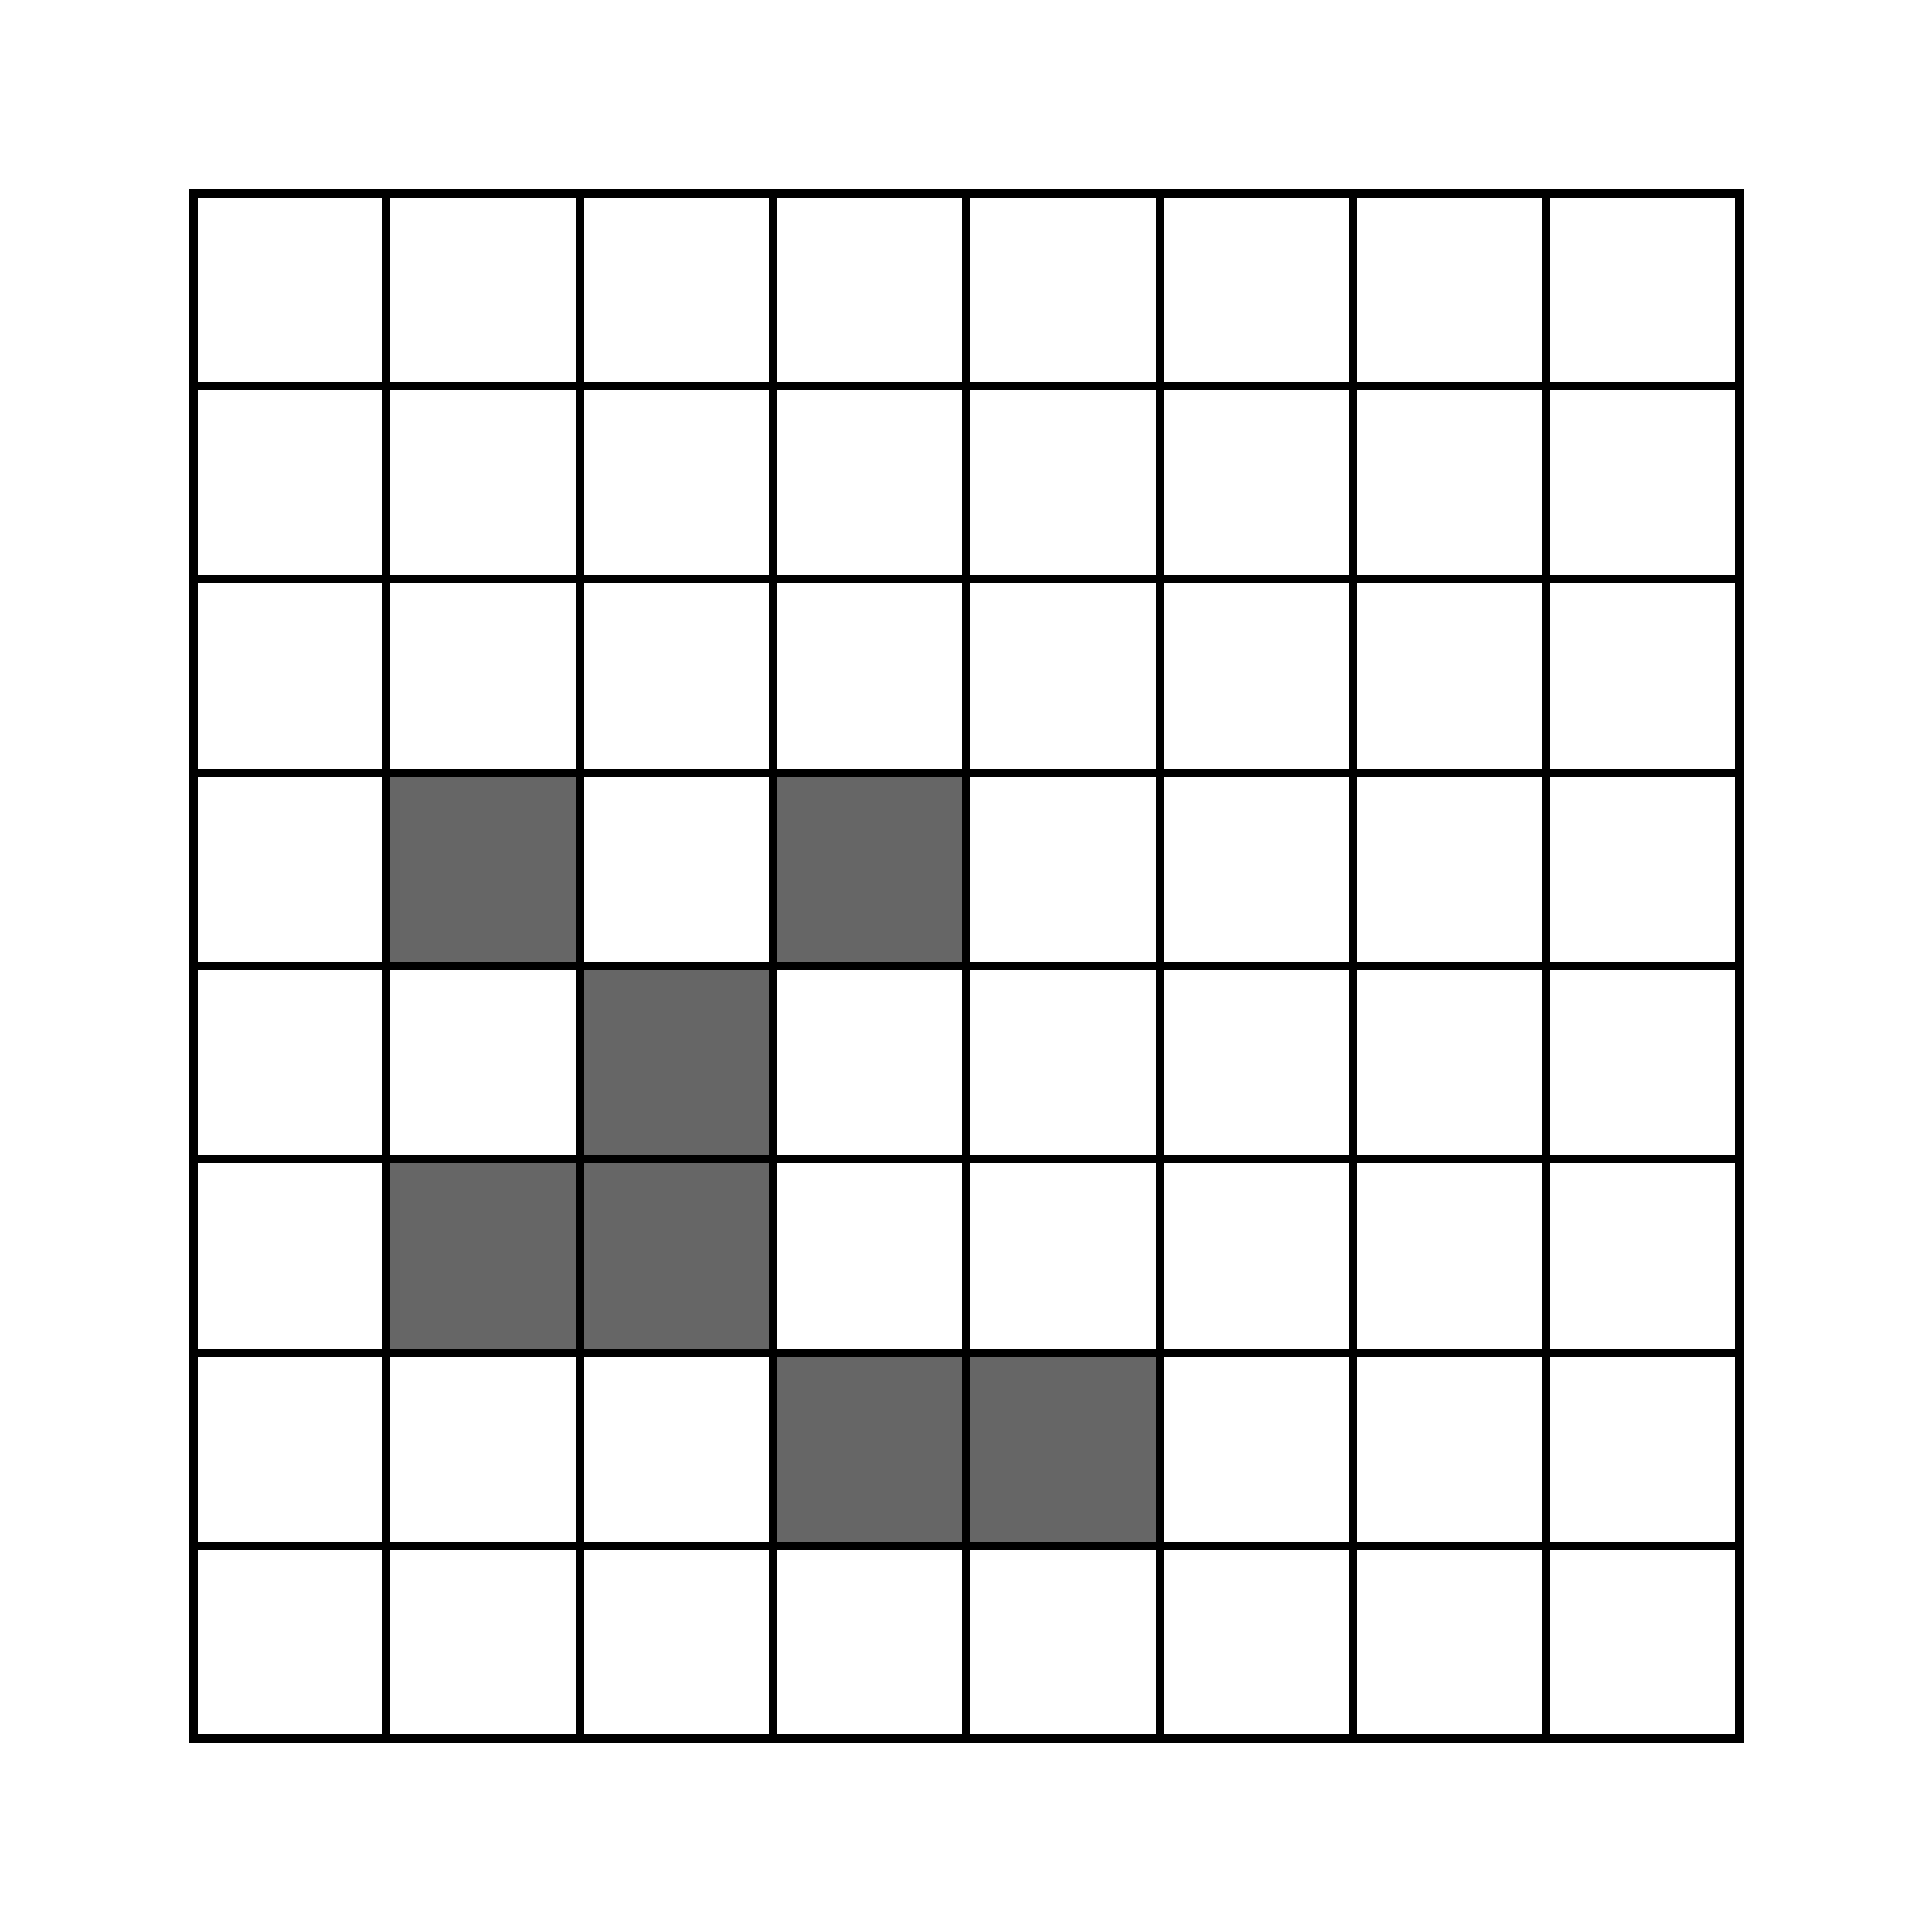
\includegraphics[width=0.2\textwidth]{chapters/cellularautomaton_images/Life4}
	\label{fig:ca_life_four_steps_step4}
}
\caption[Example of state evolution in \emph{Conway's Game of Life}]{\label{fig:ca_life_four_steps}The first four states of a \ac{CA} following the rules of \emph{Conway's Game of Life}. Grey squares represent live cells, white squares represent dead cells. The initial pattern results in complex states as the system evolves.}
\end{figure}

%% --------------------------------------------------
%% SECTION: Cellular Automata & Track Finding
%% --------------------------------------------------
\section{Cellular Automata \& Track Finding}\label{sec:cellularautomaton_history}
The use of a \ac{CA} for tracking in high-energy physics was proposed in \citep{Glazov1992} for filtering tracks in \ac{MWPC} detectors. They define a cluster of continuous hits to be a living cell and an empty region to be a dead cell. In order to support interrupted tracks due to detector inefficiencies, they also propose phantom cells, which may also be either living or dead, giving their \ac{CA} four states.

Neighbours are determined by the range of admissible angles at which a track may run through the cluster of hits corresponding to any given cell. The update rules create phantoms if there are living neighbours on either side which are compatible with the track model, and destroy cells if there are too few ($< 2$) or too many ($> 4$) neighbours. The first part is designed to cope with gaps in a track due to detector inefficiencies, while the last part filters out noise hits. The \ac{CA} is iterated until a stable configuration is reached, at which point the remaining real live cells correspond to the hits of filtered tracks. A similar procedure is also proposed in \citep{Casolino1995}.

An important development was made in \citep{Kisel1997} where it was proposed to make a \ac{CA} in which the cells were straight line segments linking hits or clusters in adjacent layers of a detector (or skipping at most one layer, to account for detector inefficiencies). The neighbours of a cell are considered to be those cells which share a hit or cluster at one end and have some angle $\phi < \phi_\mathrm{max}$ between the line segments.

An integer number is assigned as the state of each cell, associated with the cell's position along the track. Initially, all cells get the state 1 and at each step of evolution the update rule looks at neighbours in preceding layers and increases the position value by 1 if there is a neighbouring cell with the same state. Evolution stops when no neighbouring cells have the same state. As usual, time evolves in discrete steps with cell updates occurring simultaneously.

After this \ac{CA} is run the final state gives the positions of all segments of all track candidates. The track candidates are formed by starting with the highest valued segments and adding the neighbour with the previous position value, all the way back to position value 1. This approach not only filters out noise but also \emph{clusters} the track candidates into distinct clusters.

A further example of the use of line segments for the cells of a \ac{CA} with similar update rules, considering neighbours to be leftward segments sharing a common space point and having some angle no greater than a maximum \emph{breaking angle} between adjacent segments is considered for the HERA-B vertex detector in \citep{Abt2002}. The approach is extended to 3D tracks in a layered scintillator bar detector with horizontal and vertical layers in \citep{Maesaka2005}, where the \ac{CA} is run in 2D over the $xz$-plane and the $yz$-plane independently, and tracks are combined into a three-dimensional reconstruction using $z$ positions and timing information.

%% --------------------------------------------------
%% SECTION: 3D Cellular Automaton for Track Finding
%% --------------------------------------------------
\section{A 3D Cellular Automaton for Track Finding}\label{sec:cellularautomaton_algorithm}
The \ac{CARLA} algorithm is composed of several procedures, each of which is described in detail. The algorithm runs through each of the following stages in turn:

\begin{enumerate}
	\item Preprocessing
	\item Cell generation
	\item Forward run
	\item Reverse run
	\item Postprocessing
\end{enumerate}

The pre- and post-processing stages are specific to the form of data used; preprocessing typically includes a charge weighting process followed by a re-scaling to reduce the number of input hits, while postprocessing typically involves merging track segments and filtering out short fragments. In the following algorithm descriptions, the term \emph{leftward} means having lower coordinate value along the beam axis, which is defined to be the $x$-axis in the simulation. Similarly, \emph{rightward} means having higher coordinate value along the beam axis.

%% --------------------------------------------------
%% SUBSECTION: Preprocessing
%% --------------------------------------------------
\subsection{Preprocessing}\label{sec:cellularautomaton_preprocessing}
\subsubsection{Charge Weighting}\label{sec:cellularautomaton_preprocessing_charge_weighting}
A charge weighted smoothing procedure is applied to the raw hits before further processing occurs. This procedure is described in section \ref{sec:cellularautomaton_charge_weighting}.

\subsubsection{Scaling}\label{sec:cellularautomaton_scaling}
The run time of the \ac{CA} depends strongly on the hit multiplicity (which in turn determines the cell multiplicity). In order to reduce the run time, a re-scaling from $1\mm$ to $3\mm$ voxels is implemented after the charge weighting procedure. This re-scaling groups together hits within the same $3\mm \times 3\mm \times 3\mm$ region and represents them as a single cluster at the charge-weighted centroid position of those hits (calculated as for the charge weighting, with equation \ref{eqn:charge_weighted_avg_position}), but now containing the accumulated charge of all the hits within it.

%% --------------------------------------------------
%% SUBSECTION: Cell Generation
%% --------------------------------------------------
\subsection{Cell Generation}\label{sec:cellularautomaton_cell_generation}
Cell generation is the process by which cells are made from pairs of hits. A cell consists of a leftward and rightward hit pair, and represents the line between the two hits, pointing from the leftward hit to the rightward hit.  In principle, each possible pairing of points within a fixed radius could produce a cell, but for speed and performance reasons it is better to build the cells more selectively. The algorithm below does this in a manner which produces the required cells with very little overhead.

For each hit in the event:
\begin{enumerate}
	\item Build a list of neighbouring hits within a $2\mm$ radius; in this implementation a \ac{KDTree} is used for this near-neighbour search.
	\item Filter the neighbour list to select only those neighbours which are \emph{upstream} with respect to the beam direction, i.e. select only leftward neighbours.
	\item Generate a cell for each remaining leftward neighbour, pointing from that hit to the current central hit (from left to right); see figure \ref{fig:cellularautomaton_cellgen_normal}.
	\item If no leftward hits were found, i.e. no cells were generated in the previous step, expand the search radius by $0.05\mm$ and repeat the procedure above until either a cell is generated or the maximum search radius of $5.0\mm$ is reached; see figure \ref{fig:cellularautomaton_cellgen_expand}.
	\item If multiple cells were generated, filter out longer copies of cells with the same slope, using a comparison tolerance of $0.10$ on the slope components. This step avoids making long cells which ``jump'' over several shorter cells, which could lead to multiple interleaved tracks in the final reconstruction; see figure \ref{fig:cellularautomaton_cellgen_filter}.
\end{enumerate}

\begin{figure}
\centering
\subfigure[Normal operation]{\label{fig:cellularautomaton_cellgen_normal}
	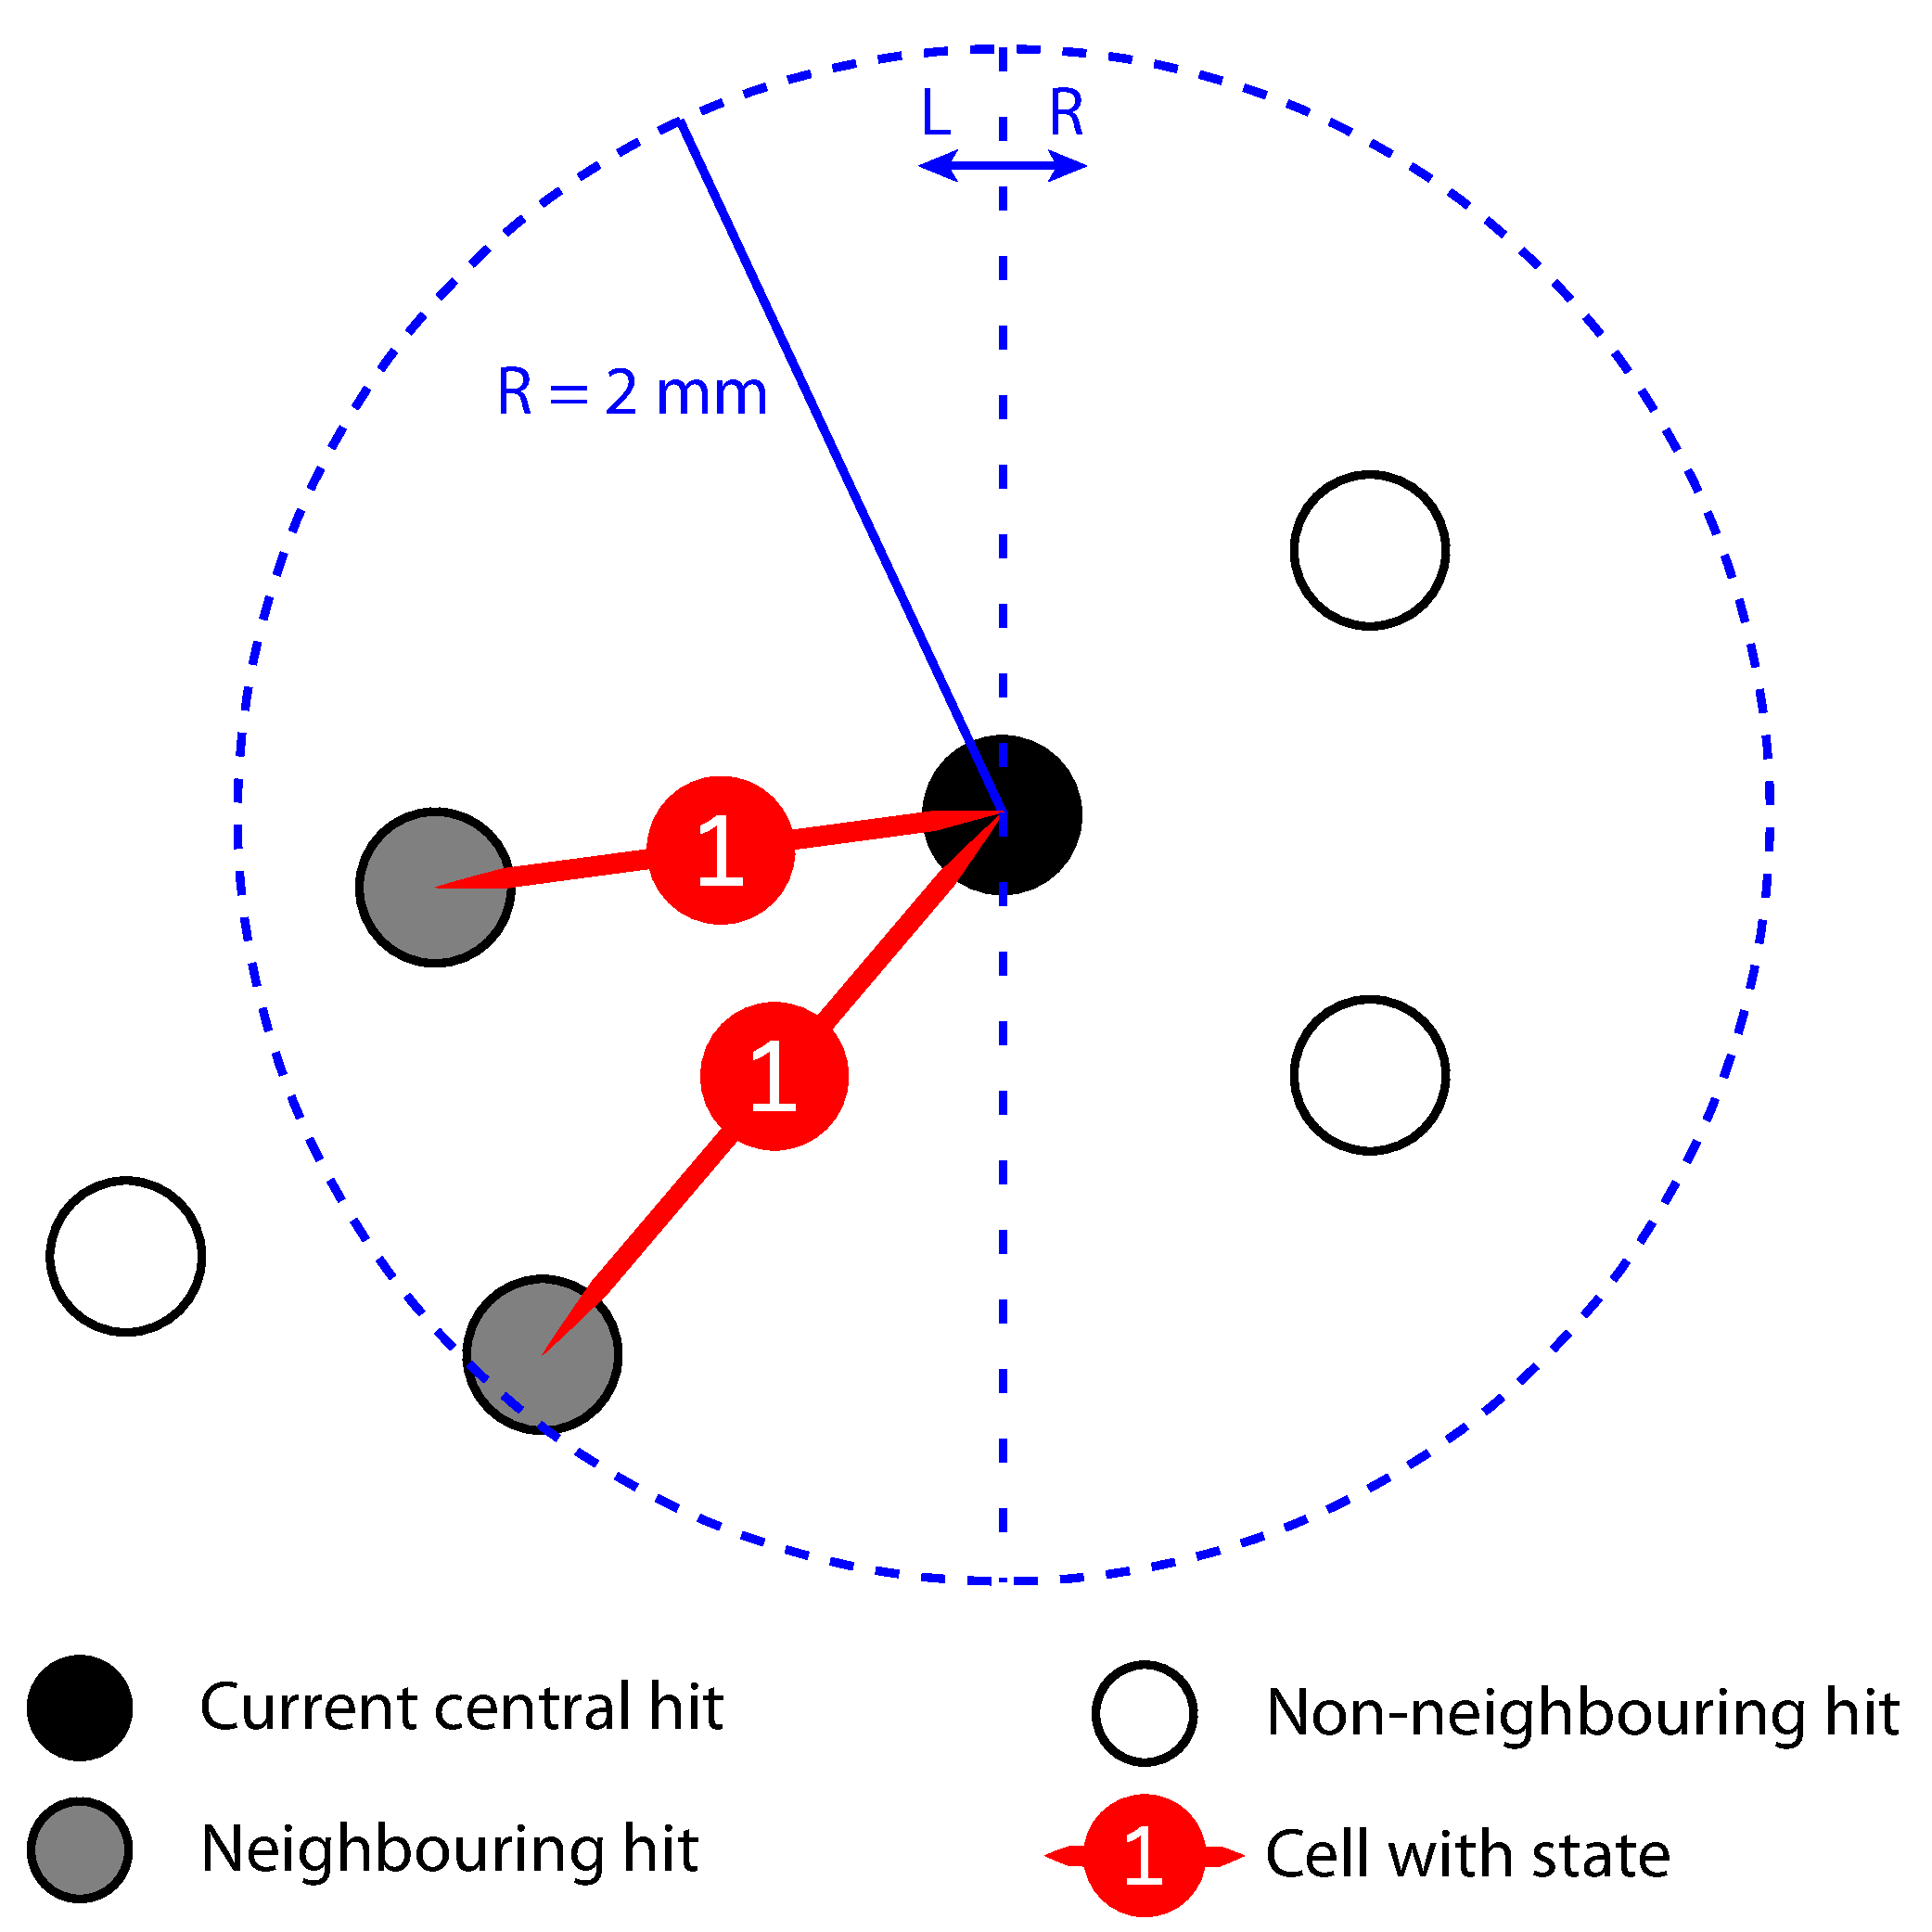
\includegraphics[width=0.3\textwidth]{chapters/cellularautomaton_images/CellGeneration1}
}
\subfigure[Expanding radius]{\label{fig:cellularautomaton_cellgen_expand}
	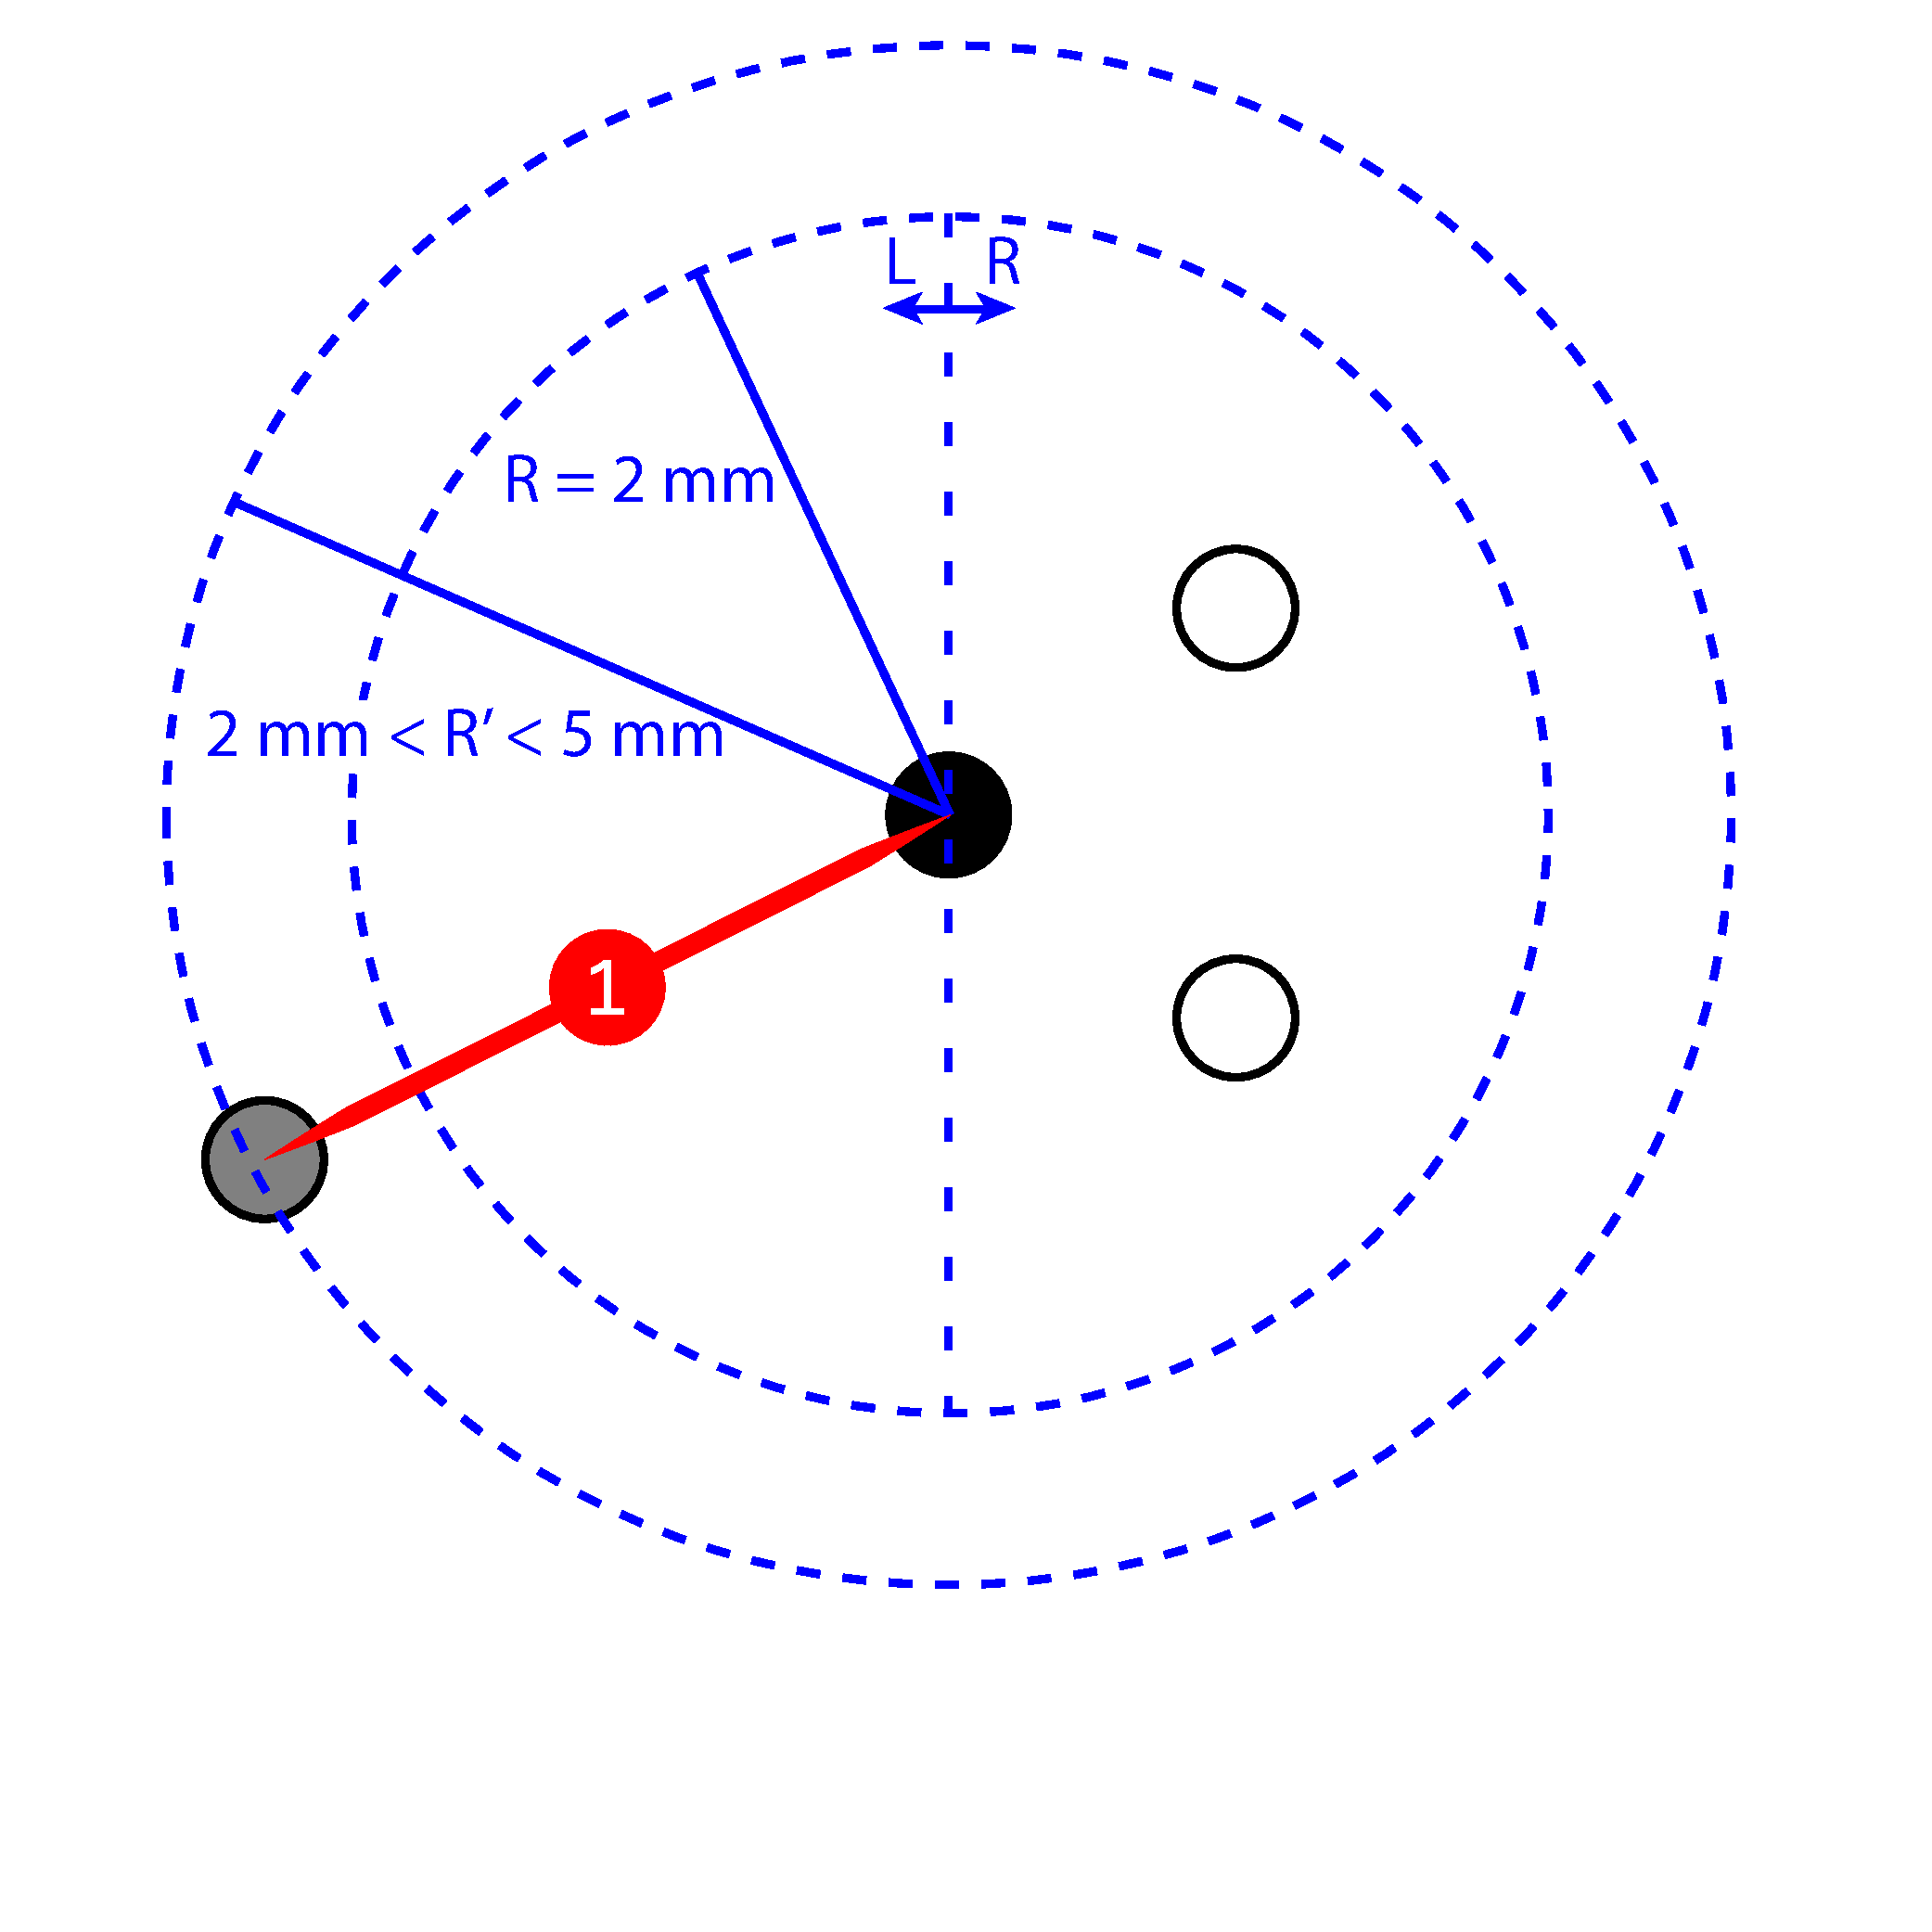
\includegraphics[width=0.3\textwidth]{chapters/cellularautomaton_images/CellGeneration2}
}
\subfigure[Filtering]{\label{fig:cellularautomaton_cellgen_filter}
	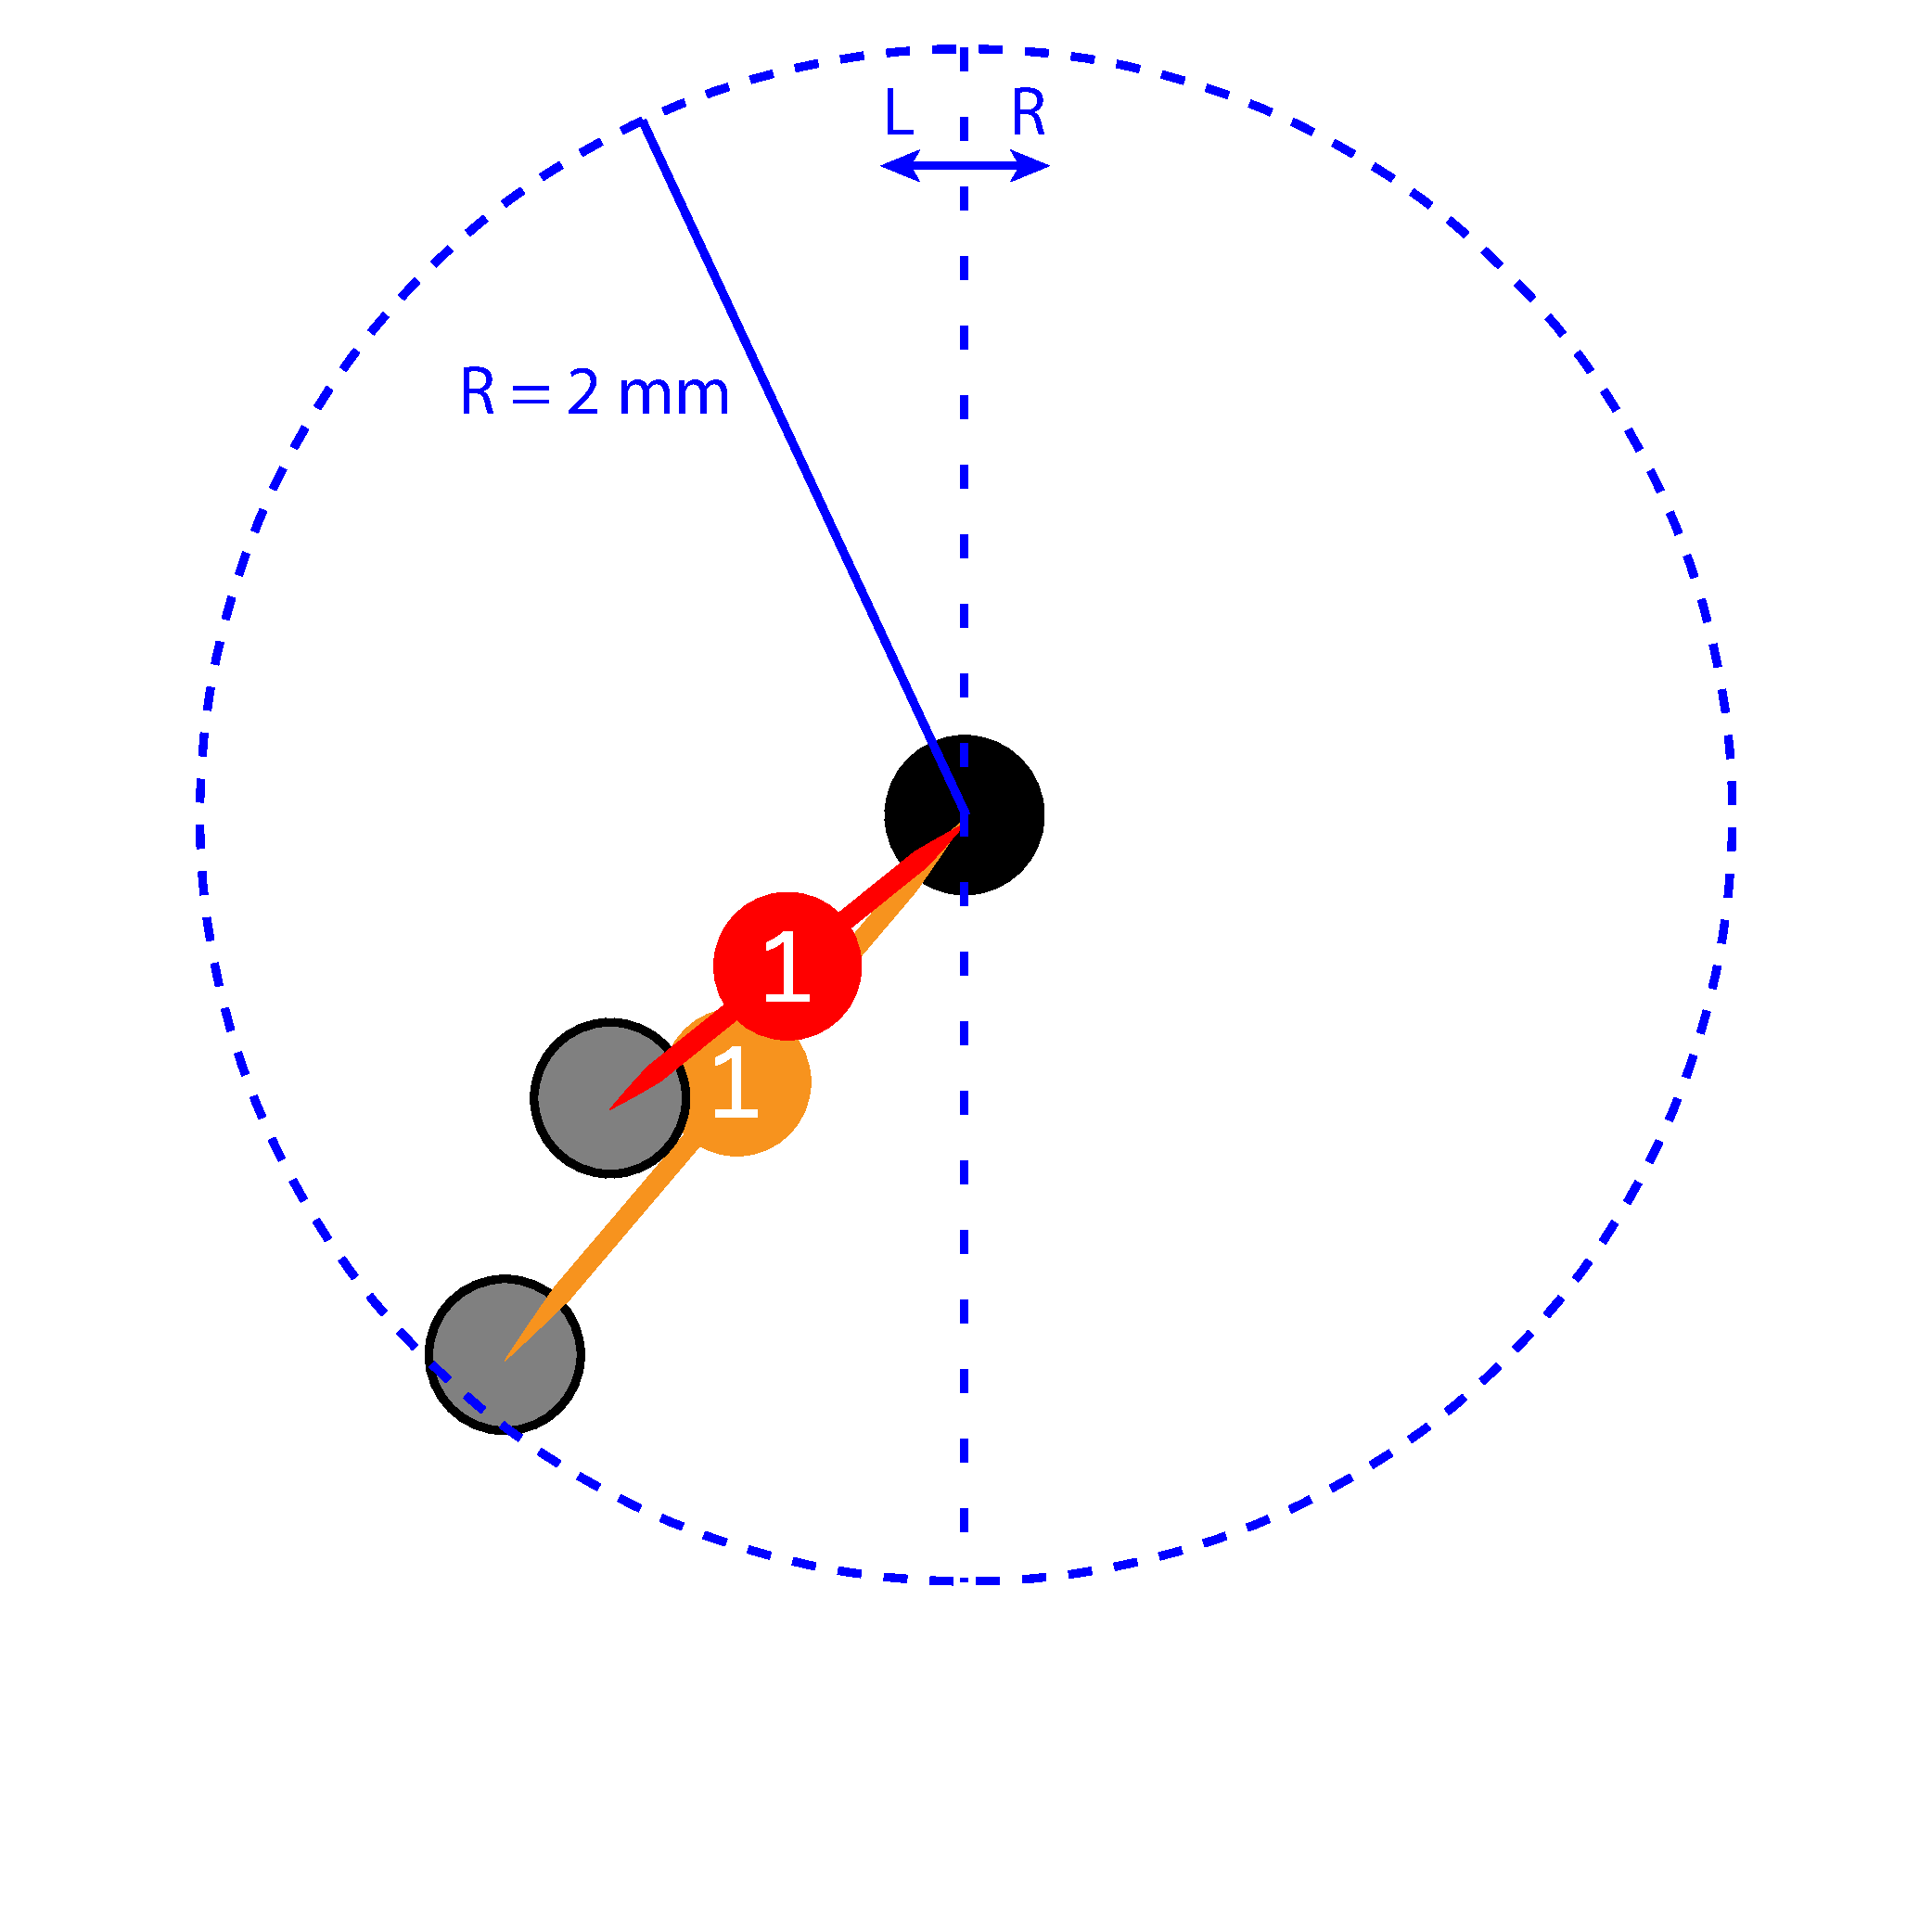
\includegraphics[width=0.3\textwidth]{chapters/cellularautomaton_images/CellGeneration3}
}
\caption[Illustration of the cell generation procedure in the CA algorithm]{\label{fig:cellularautomaton_cellgen}Illustration of the steps in the cell generation procedure for the \ac{CA}:\newline \subref{fig:cellularautomaton_cellgen_normal} creation of cells between a central point and any leftward neighbours within a $2\mm$ radius. \subref{fig:cellularautomaton_cellgen_expand} adaptive search radius expansion, which gradually expands the radius in $0.05\mm$ increments until either a leftward neighbour is found or a maximum radius of $5\mm$ is reached. \subref{fig:cellularautomaton_cellgen_filter} removal of cells if a shorter cell exists with similar slope; in this case, the red cell is retained while the longer orange cell is removed.}
\end{figure}

%% --------------------------------------------------
%% SUBSECTION: Forward Run
%% --------------------------------------------------
\subsection{Forward Run}\label{sec:cellularautomaton_forward_run}
The forward run is responsible for the evolution of the \ac{CA} from its initial state until a stable final state is reached. The forward step algorithm is run until the state remains unchanged, that is, until no cells needed to be updated in a step.

Before the first forward step, a mapping from cell to list of leftward neigbours is built. Cell A is a leftward neighbour of cell B if they share a central point (cell A's right point is identical to cell B's left point) and if the angle $\theta$ made between the two cell vectors is less than some threshold value $\theta_\mathrm{max}$. This mapping is used in every forward step, providing a speed boost over searching for leftward neighbours every time, since the number of cells does not change, and the cell properties are fixed (with the exception of cell state).

The forward step algorithm proceeds as follows (see also the illustration in figure \ref{fig:cellularautomaton_run}):
\begin{enumerate}
	\item For each cell with one or more leftward neighbours in the same state, mark the cell for update.
	\item Update all marked cells by increasing the value of their state by 1.
	\item Return the number of updated cells (if 0, this signals termination of the forward run).
\end{enumerate}

It is important not to update any cell state before all cells have been tested to see whether they must be updated. This prevents problems where a cell which would have been updated (because it had a neighbour with the same state) does not get updated because its neighbour was updated first. The forward step must appear to occur simultaneously across all cells; this opens up opportunities for parallelisation since each cell can be tested and marked for update independently. However, since this part of the algorithm is relatively quick for small numbers of cells, the current implementation does not do this in parallel.

\begin{figure}
\centering
\subfigure[Initial state]{\label{fig:cellularautomaton_run_initial}
	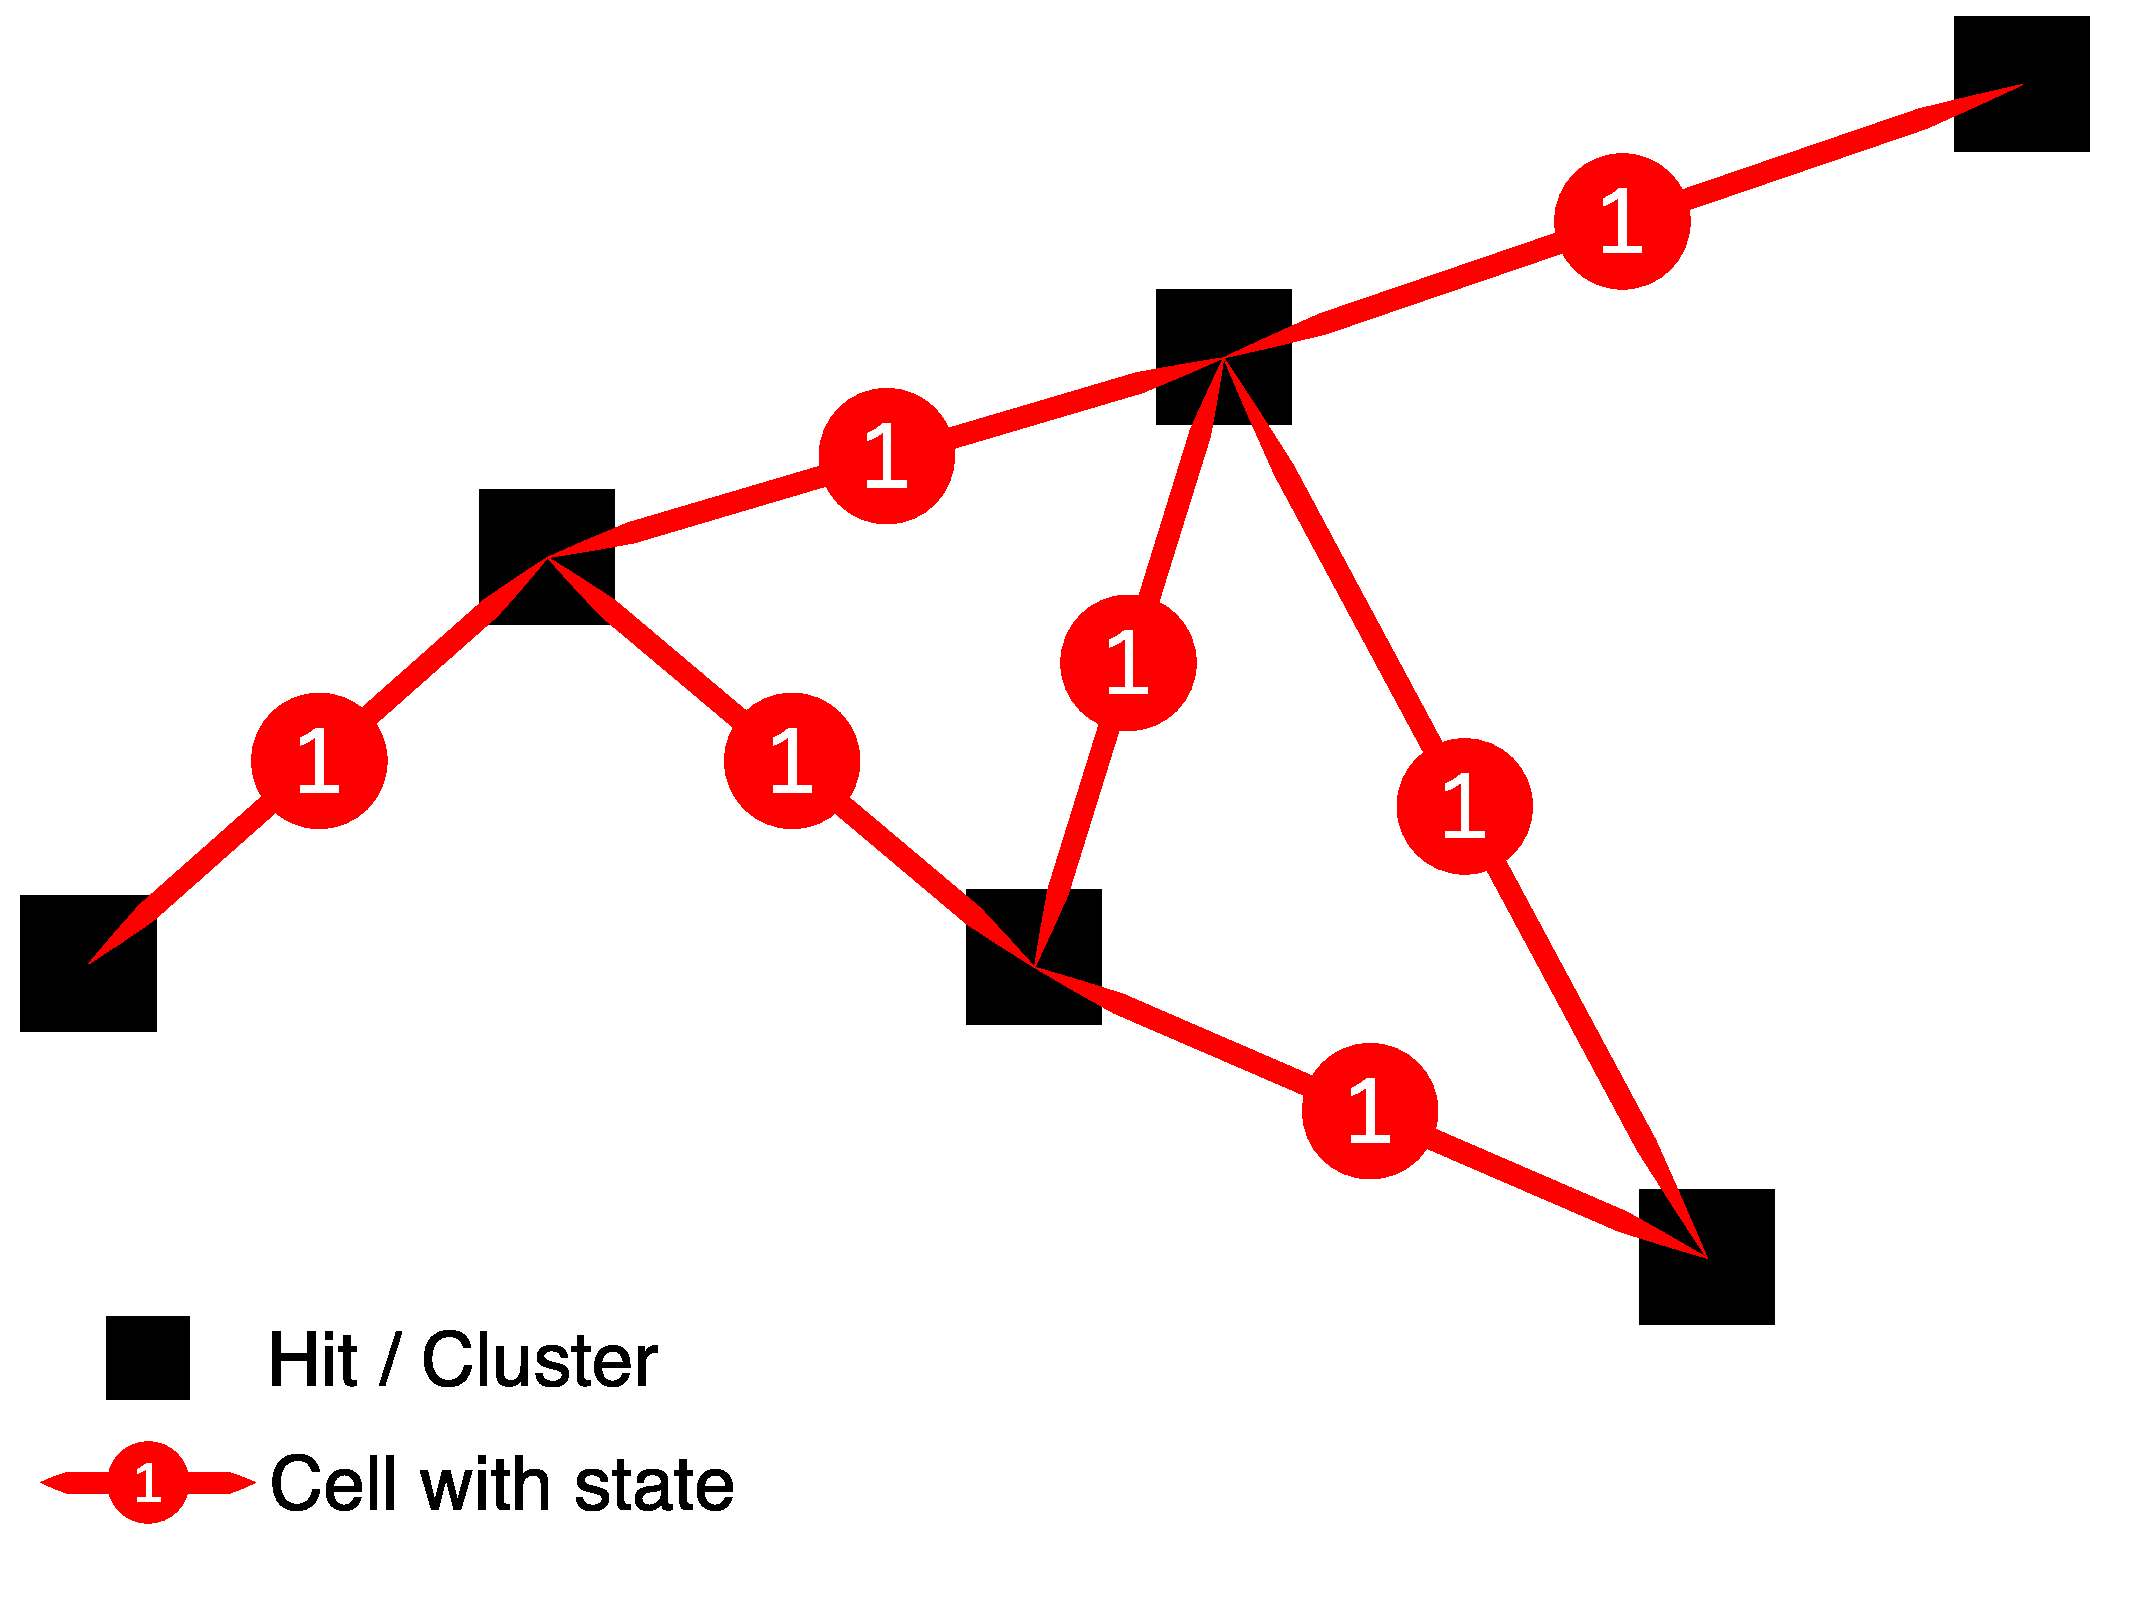
\includegraphics[width=0.3\textwidth]{chapters/cellularautomaton_images/ca-fig1}
}
\subfigure[Final state]{\label{fig:cellularautomaton_run_final}
	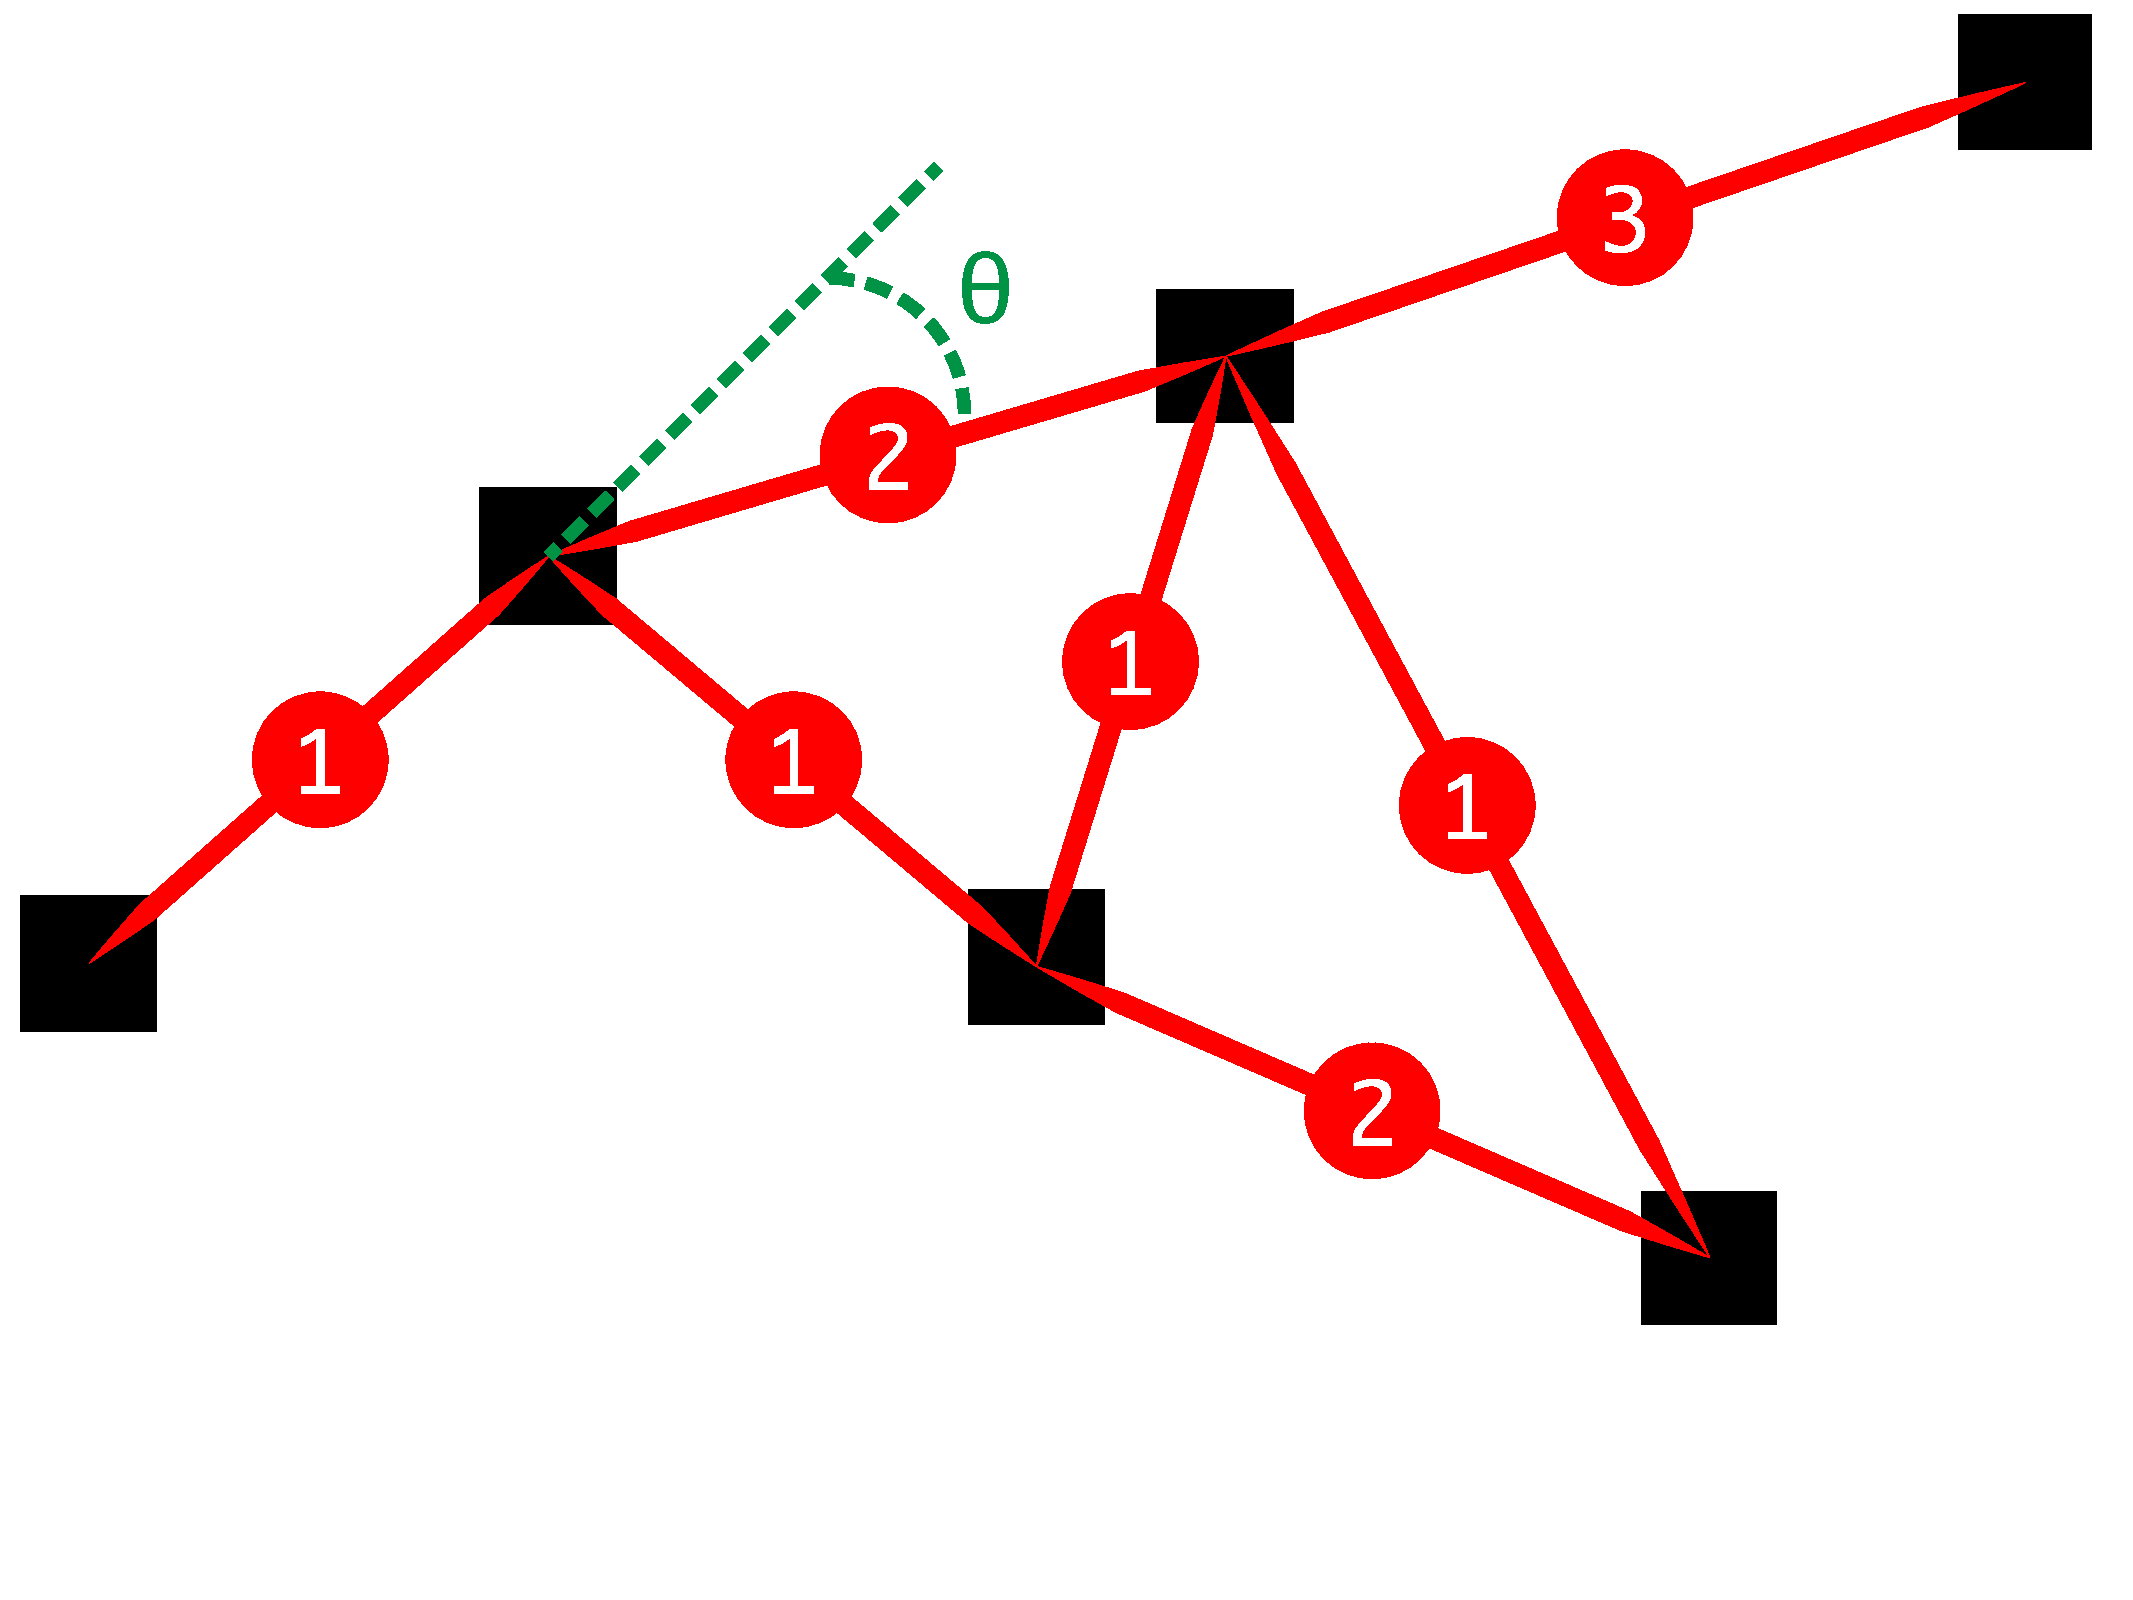
\includegraphics[width=0.3\textwidth]{chapters/cellularautomaton_images/ca-fig2-nolegend}
}
\subfigure[Output clustering]{\label{fig:cellularautomaton_run_output}
	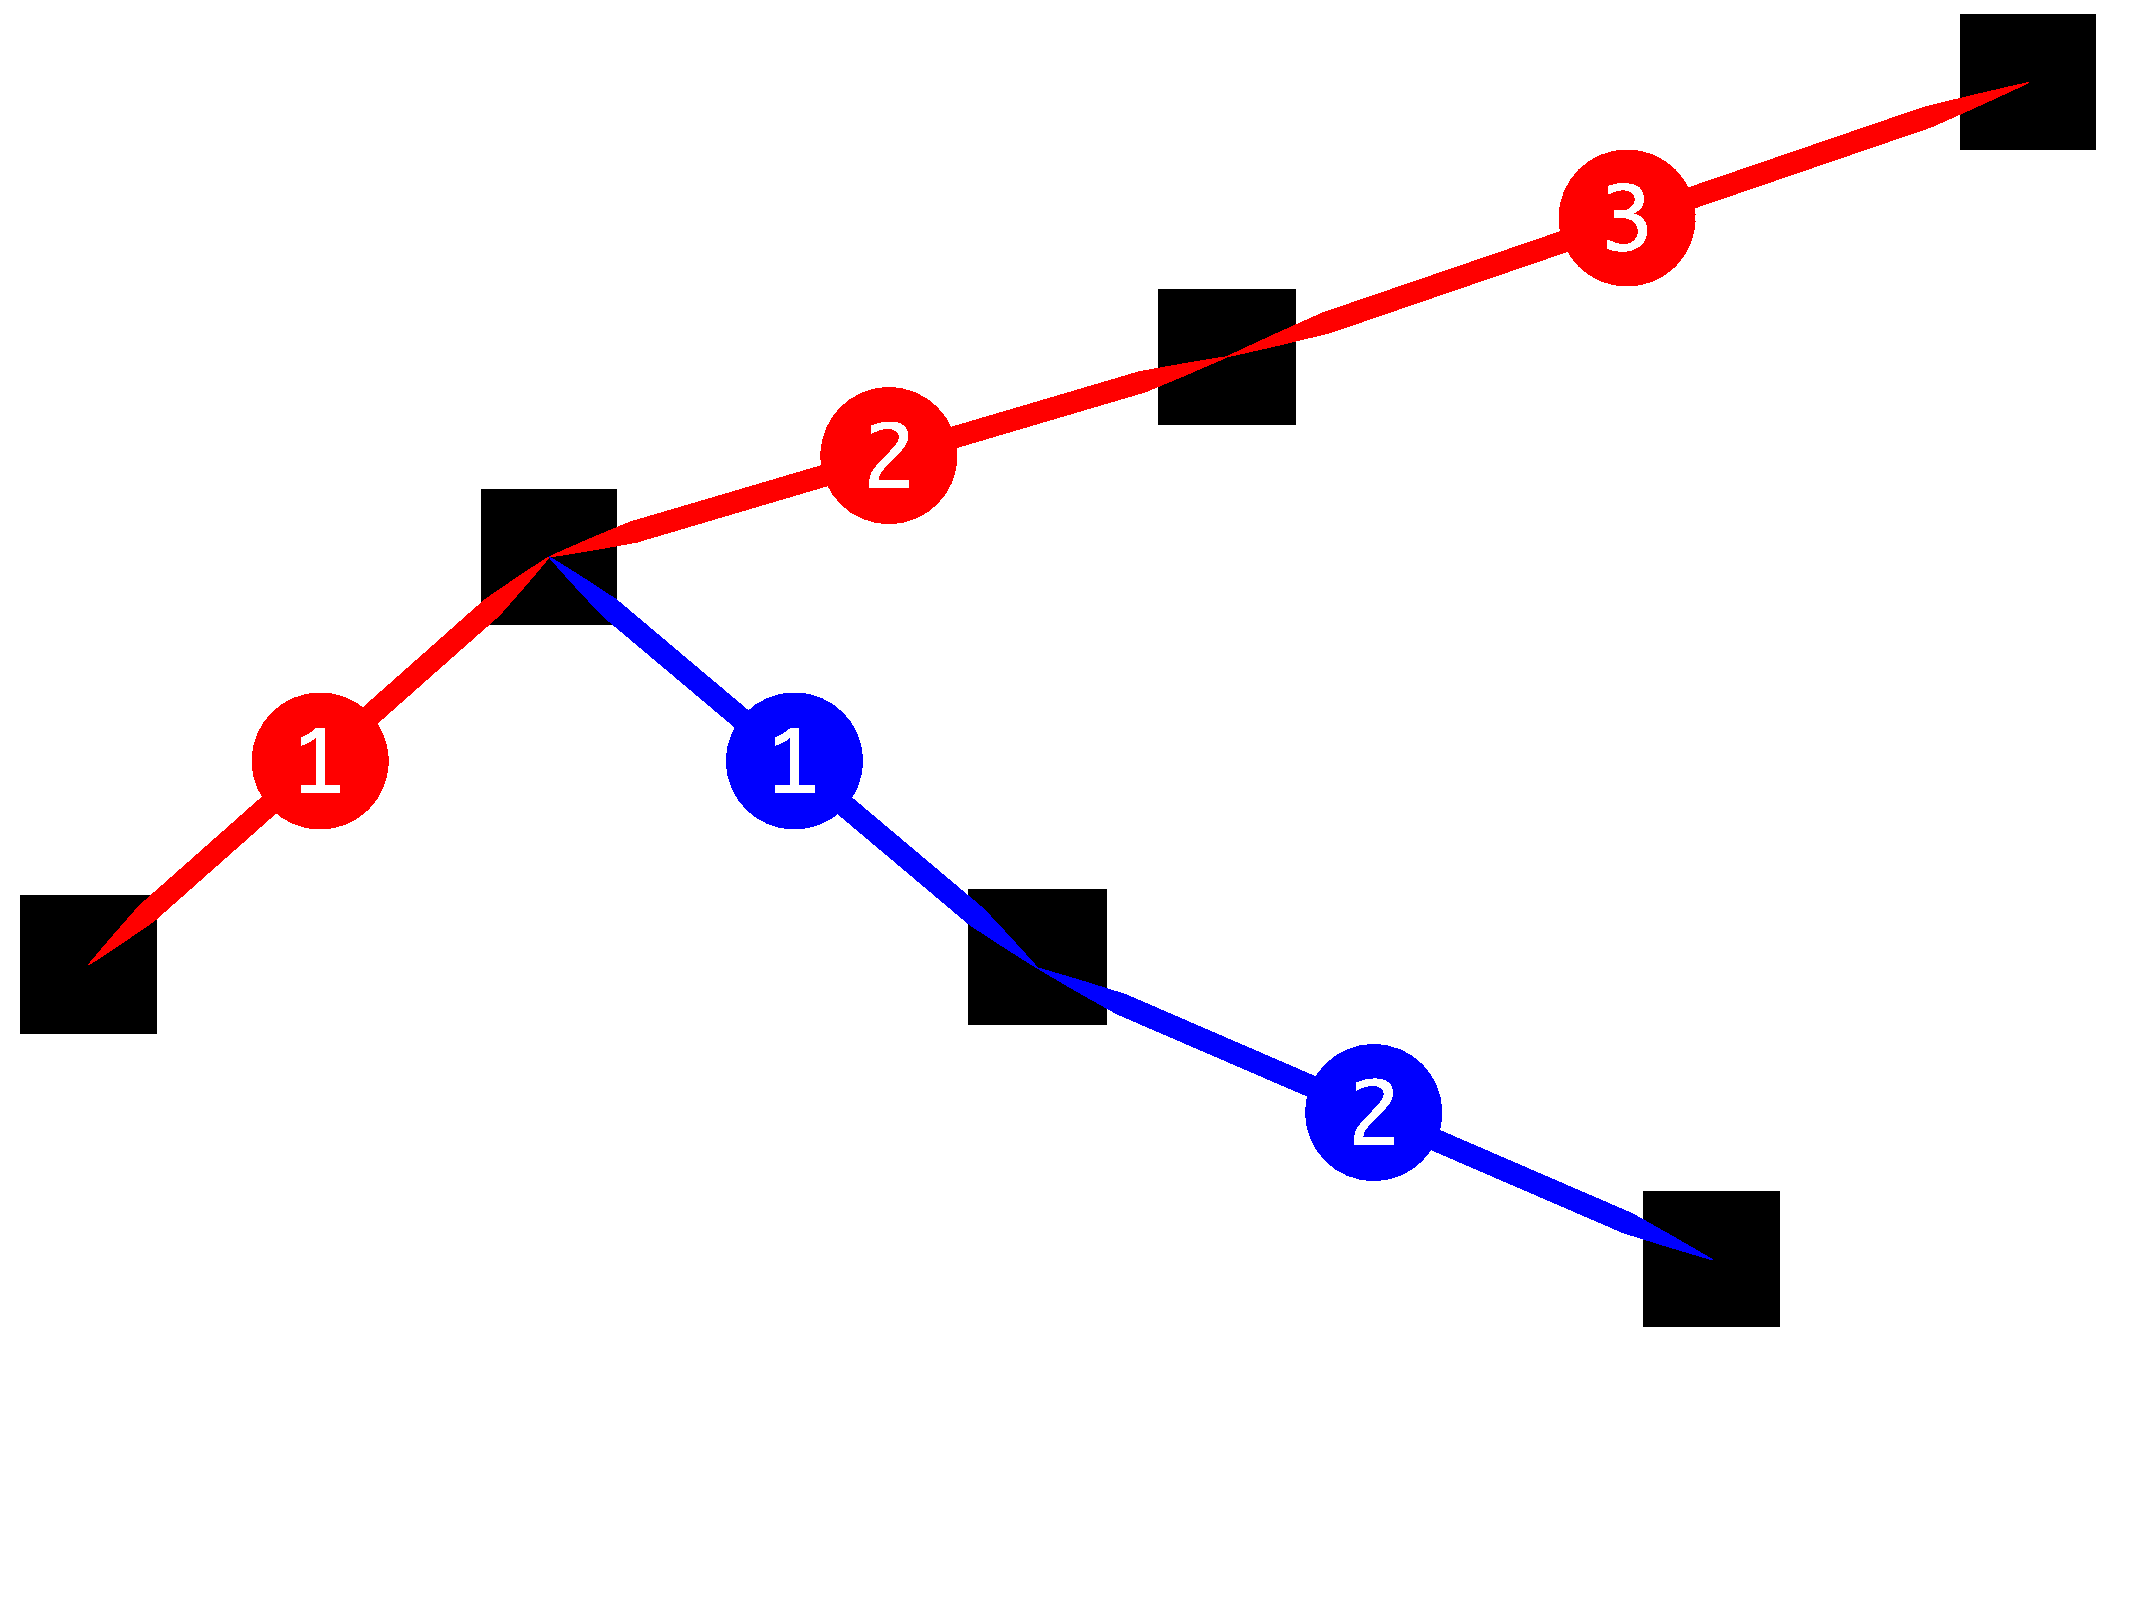
\includegraphics[width=0.3\textwidth]{chapters/cellularautomaton_images/ca-fig3-nolegend}
}

\caption[Initial and final states of a CA for track finding]{\label{fig:cellularautomaton_run}Illustration of the effects of the forward run of a \ac{CA} on a set of cells:\newline \subref{fig:cellularautomaton_run_initial} initial state with all cell values set to 1. \subref{fig:cellularautomaton_run_final} final state where cell values have been updated as per the forward step algorithm. Cell values now reflect the position of a cell in a straight line track. Cells which have no leftward neighbours consistent with the breaking angle $\theta$ retain the value 1. \subref{fig:cellularautomaton_run_output} track clusters are formed by following chains from high-valued to low-valued cells, while cells which are not part of a track are filtered out.}
\end{figure}

%% --------------------------------------------------
%% SUBSECTION: Reverse Run
%% --------------------------------------------------
\subsection{Reverse Run}\label{sec:cellularautomaton_reverse_run}
The reverse run extracts track clustering information from the final state of the \ac{CA}. The mapping of cells to a list of their leftward neighbours is retained, again for efficiency. Initially, all cells are considered as input to the reverse run. The reverse step algorithm is performed until no cells remain in the input list.

The reverse step algorithm proceeds as follows:
\begin{enumerate}
	\item Find the input cell with the highest valued state. Set as current cell.
	\item Create a new track candidate and add the current cell to it.
	\item While the current cell has value $> 1$:
	\begin{enumerate}
		\item Find a leftward neighbouring cell with state value 1 less than the current cell state.
		\item If multiple candidate cells exist, pick the one which makes the smallest angle with the current cell.
		\item Add this cell to the track candidate, and mark it as the new current cell.
	\end{enumerate}
	\item Remove allocated cells from the input list.
\end{enumerate}

Each reverse step follows a sequence of cells from a high-valued cell state to a cell with state 1, building a complete track candidate in the process. The reverse step algorithm runs until all track candidates have been extracted. Track candidates which contain only 1 cell are rejected as noise. The result of applying the reverse run algorithm is illustrated in figure \ref{fig:cellularautomaton_run_output}. Finally, the cells in each track candidate are unpacked to leave each track as a list of hits.

%% --------------------------------------------------
%% SUBSECTION: Postprocessing
%% --------------------------------------------------
\subsection{Postprocessing}\label{sec:cellularautomaton_postprocessing}
The \ac{CA} algorithm is considered to be complete at this point. Postprocessing stages are used to improve the results from the \ac{CA} based on its known properties.

The first stage involves uniquely assigning hits to tracks. The \ac{CA} makes unique assignments of cells to tracks, but since a hit can appear as an endpoint of multiple cells, it is possible that hits may appear multiple times across multiple tracks. The current strategy for unique hit assignment is to keep each hit with the longest track it is a member of, and remove it from any shorter tracks.

The second stage of postprocessing merges track segments together if they are compatible with being part of the same straight line. This is necessary because the CA tends to break tracks up at any site of complexity, including the primary vertex, decay vertices and delta electron production sites. In particular for $\mu$ tracks, it is useful to stitch together these segments to produce a single longer track. The merging algorithm is described in detail in section \ref{sec:cellularautomaton_merging}

%% --------------------------------------------------
%% SECTION: Performance of the CA on Toy MC Events
%% --------------------------------------------------
\section{Performance of the \acl{CA} on Toy Monte Carlo Events}\label{sec:ca-toy-tracks}
The \ac{CA} was initially tested on a set of straight line tracks from a toy \ac{MC} generator which deposits charge from straight line segments in voxels of $1\mm\times1\mm\times1\mm$. The tracks are generated such that they have lengths between $200\mm$ and $300\mm$. Both tracks begin at point $(0, 0, 0)$, and the opening angle between the two tracks is fixed to some $\theta$. The events are then rotated so that the lines are distributed isotropically, but retain the fixed opening angle and start point. A thousand events were generated at each angle $\theta$ from $2\degree$ to $178\degree$ in $4\degree$ intervals.

The events were first charge weighted with a radius of $6.0\mm$, then scaled with a scale size of $3.0\mm$. The resulting hits were run through the cell generation process with a default cell generation radius of $6.0\mm$, maximum radius $15.0\mm$ (in unscaled units). The \ac{CA} algorithm itself was applied with a breaking angle $\theta_\mathrm{max} = 10\degree$ and the resulting tracks were postprocessed with the track road merging algorithm with a cylinder radius of $5.0\mm$.\footnote{These parameters were chosen in order to maximise the number of correctly reconstructed events.}

%% --------------------------------------------------
%% SUBSECTION: Raw CA output
%% --------------------------------------------------
\subsection{Raw \acl{CA} Output}
The number of tracks found by the \ac{CA} as a function of angle is presented in figure \ref{fig:ca_toy_raw_trackcounts}. With 1000 events at each angle, and an input sample of events containing only two tracks, the number of interest is the efficiency for finding two tracks; that is, the number of events in which two clusters were found divided by the total number of events.% The two track efficiency is shown in figure \ref{fig:ca_toy_raw_twotrack_efficiency}.

\begin{figure}
\centering
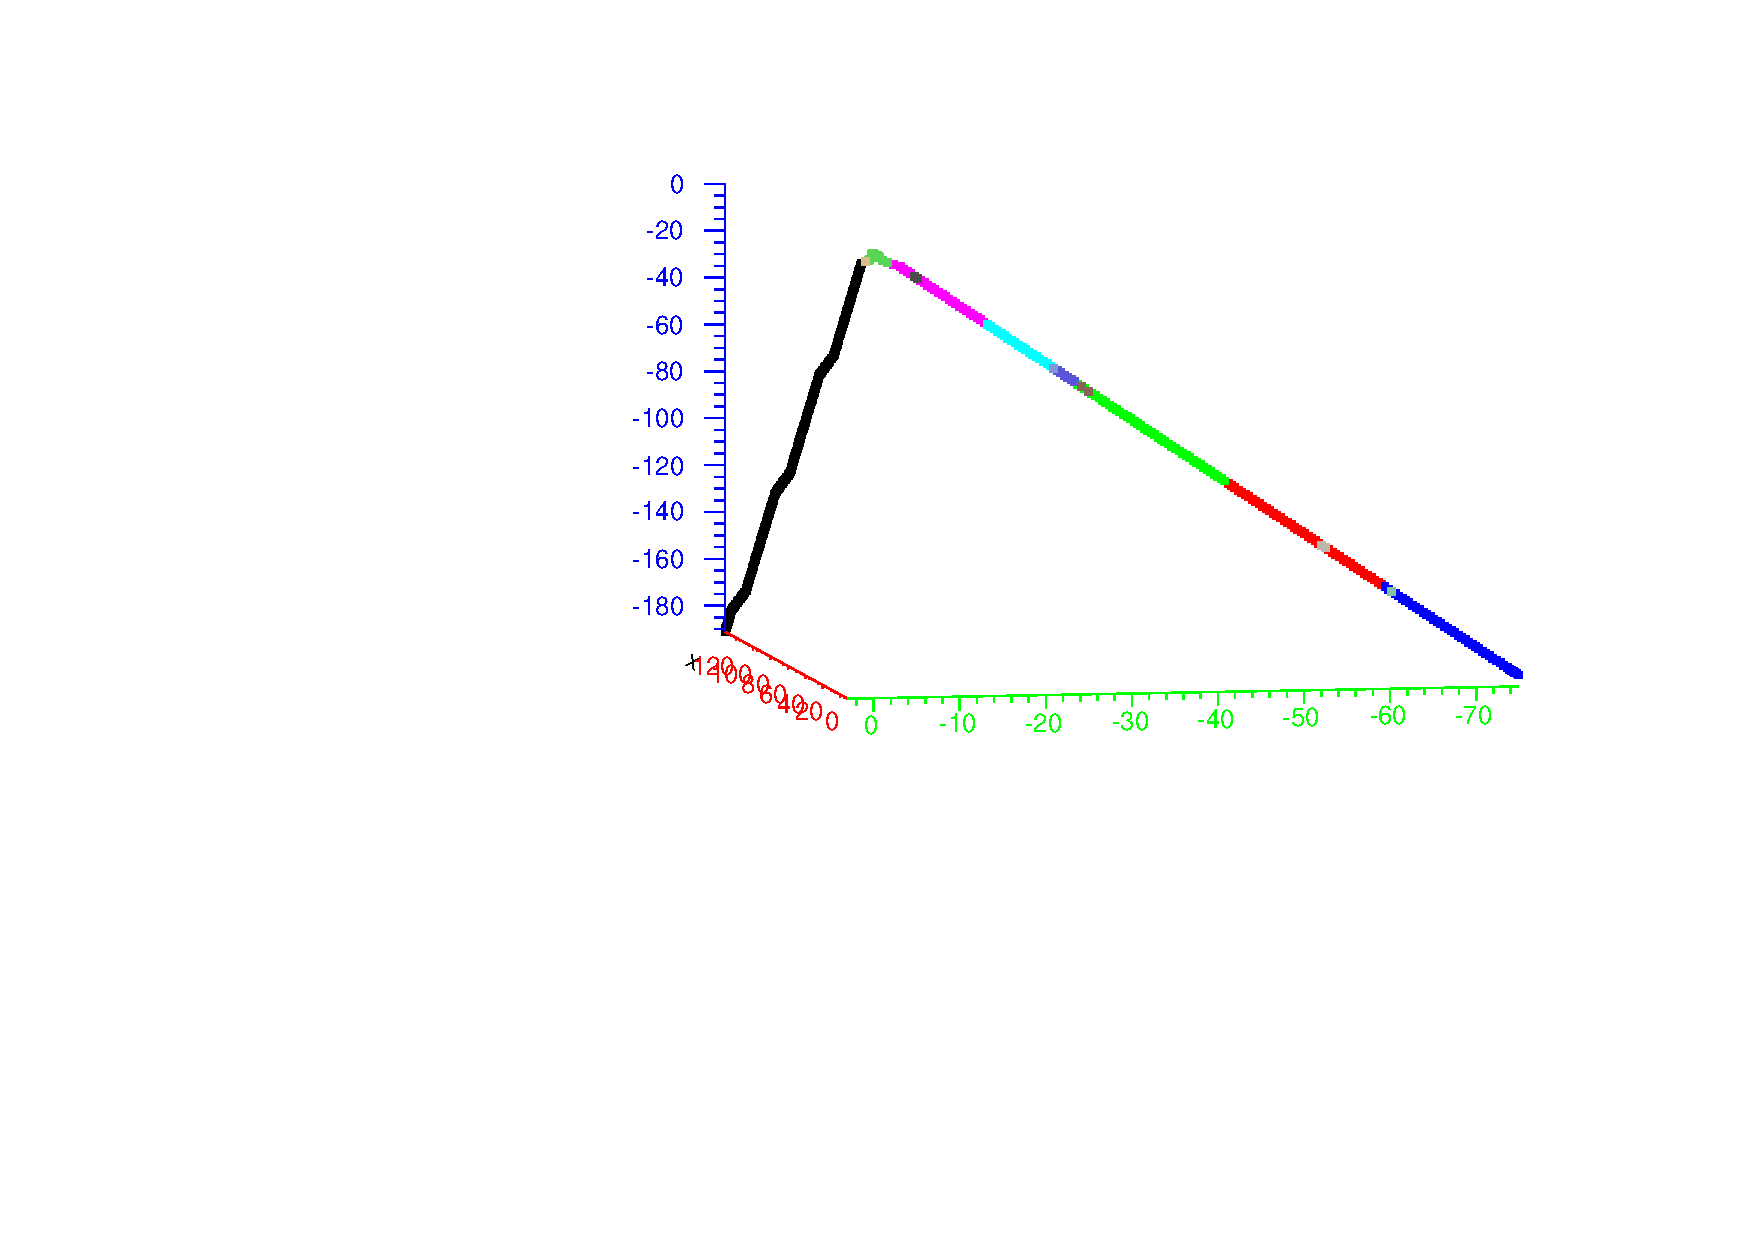
\includegraphics[angle=-90,width=0.8\textwidth]{chapters/cellularautomaton_images/openingangle-event_16-42deg}
\caption[Sample CA reconstruction of toy event with $42\degree$ opening angle]{\label{fig:ca-openingangle-sample-event-raw}Sample event from the toy track generator, with an opening angle of $42\degree$ between the two tracks. The cellular automaton clusters one track successfully, but produces several clusters (each coloured segment represents a cluster) along the length of the other due to the geometric effects of the voxellised data. It is important to note that each such cluster forms a segment along the line which is easy to merge together with the other segments, and that the segments include no hits that do not belong (i.e. hits from the other line).}
\end{figure}

\begin{figure}
\centering
% "Run8": CA Theta 10 deg, CW Radius 6 mm, Merging radius 5 mm
\resizebox{0.9\textwidth}{!}{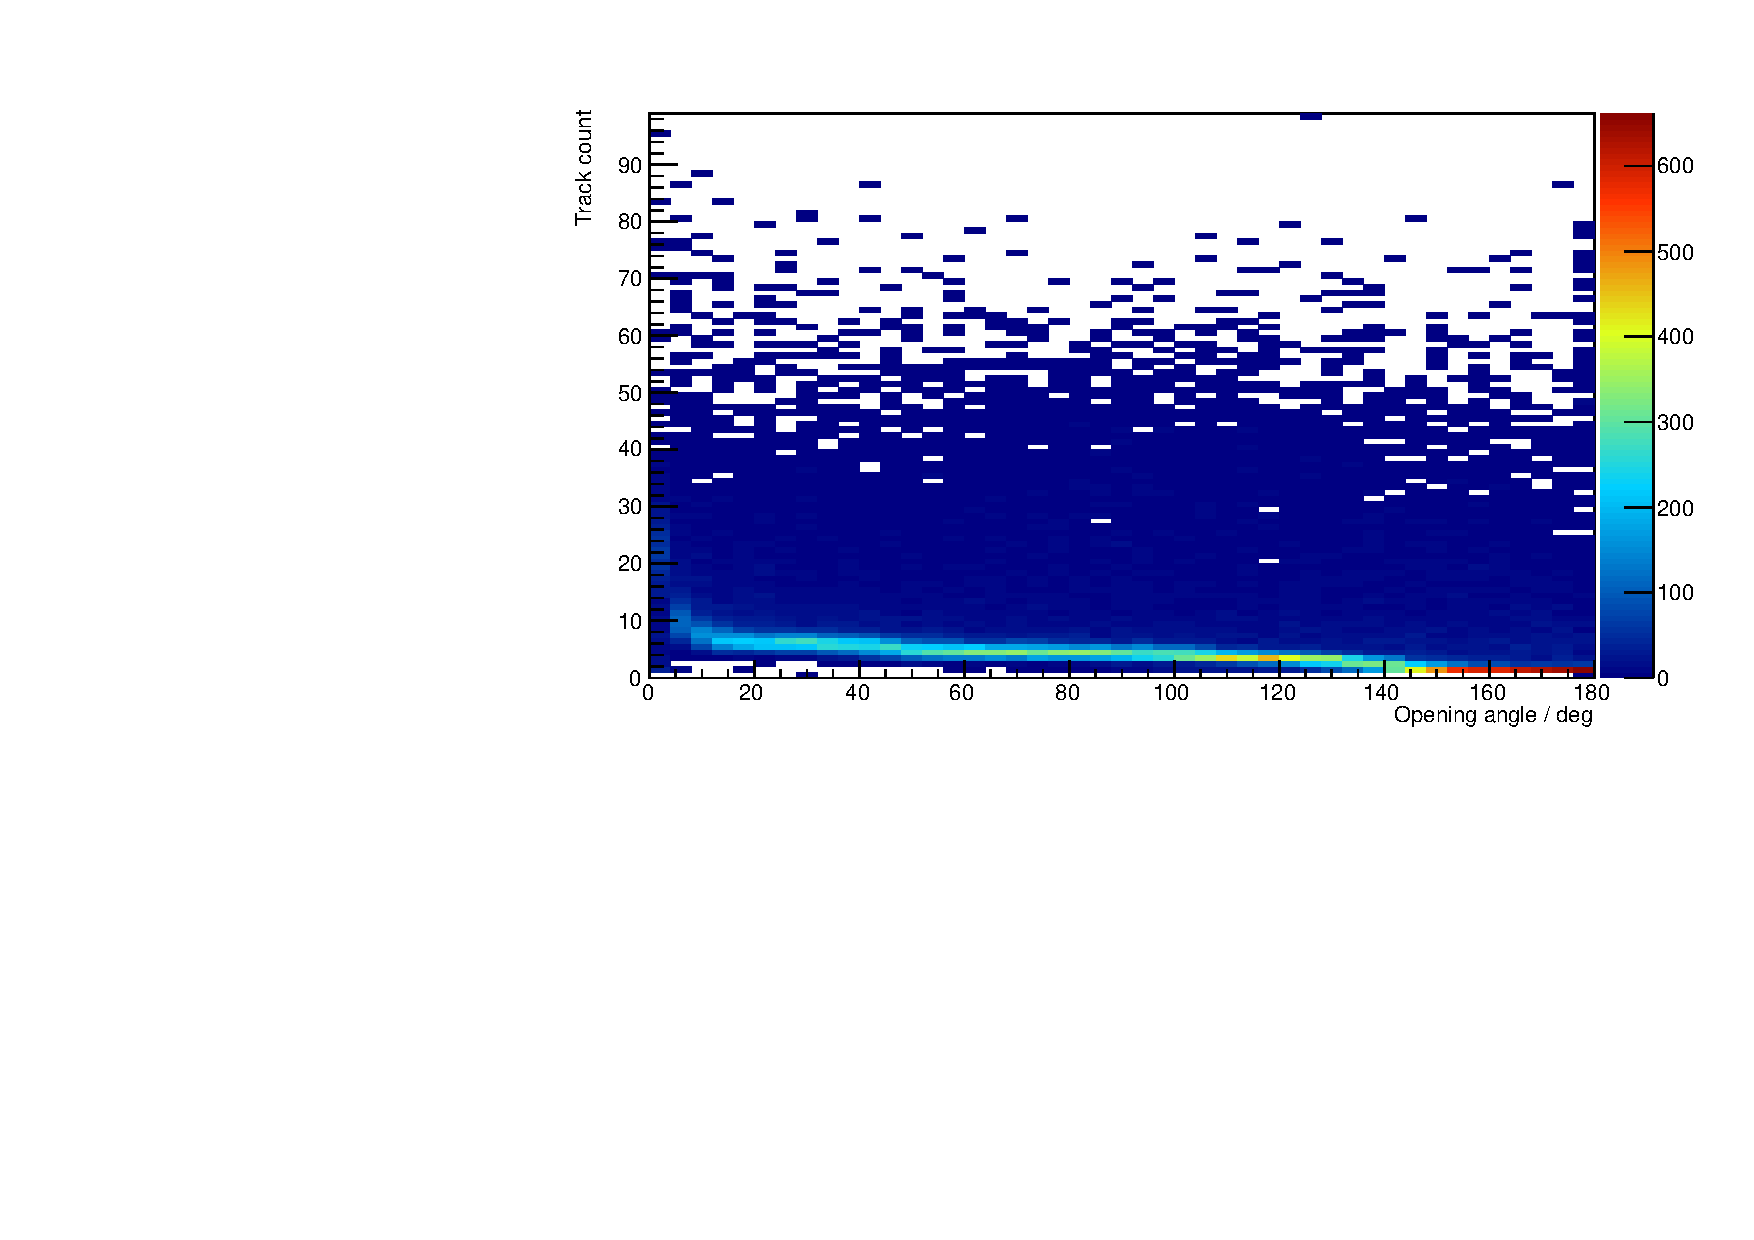
\includegraphics[angle=-90]{chapters/cellularautomaton_images/toy_raw_counts}}
\caption[Track count as a function of angle for raw CA operating on toy MC events]{\label{fig:ca_toy_raw_trackcounts}Number of tracks found as a function of opening angle for the raw \ac{CA} operating on two track events with a fixed opening angle. There are 1000 events per opening angle, and the events are rotated so as to be distributed isotropically. Large numbers of tracks are found in some cases due to geometric effects in the way the \ac{CA} operates. These can be merged back together with an appropriate merging algorithm.}
\end{figure}

%\begin{figure}
%\centering
%\resizebox{0.9\textwidth}{!}{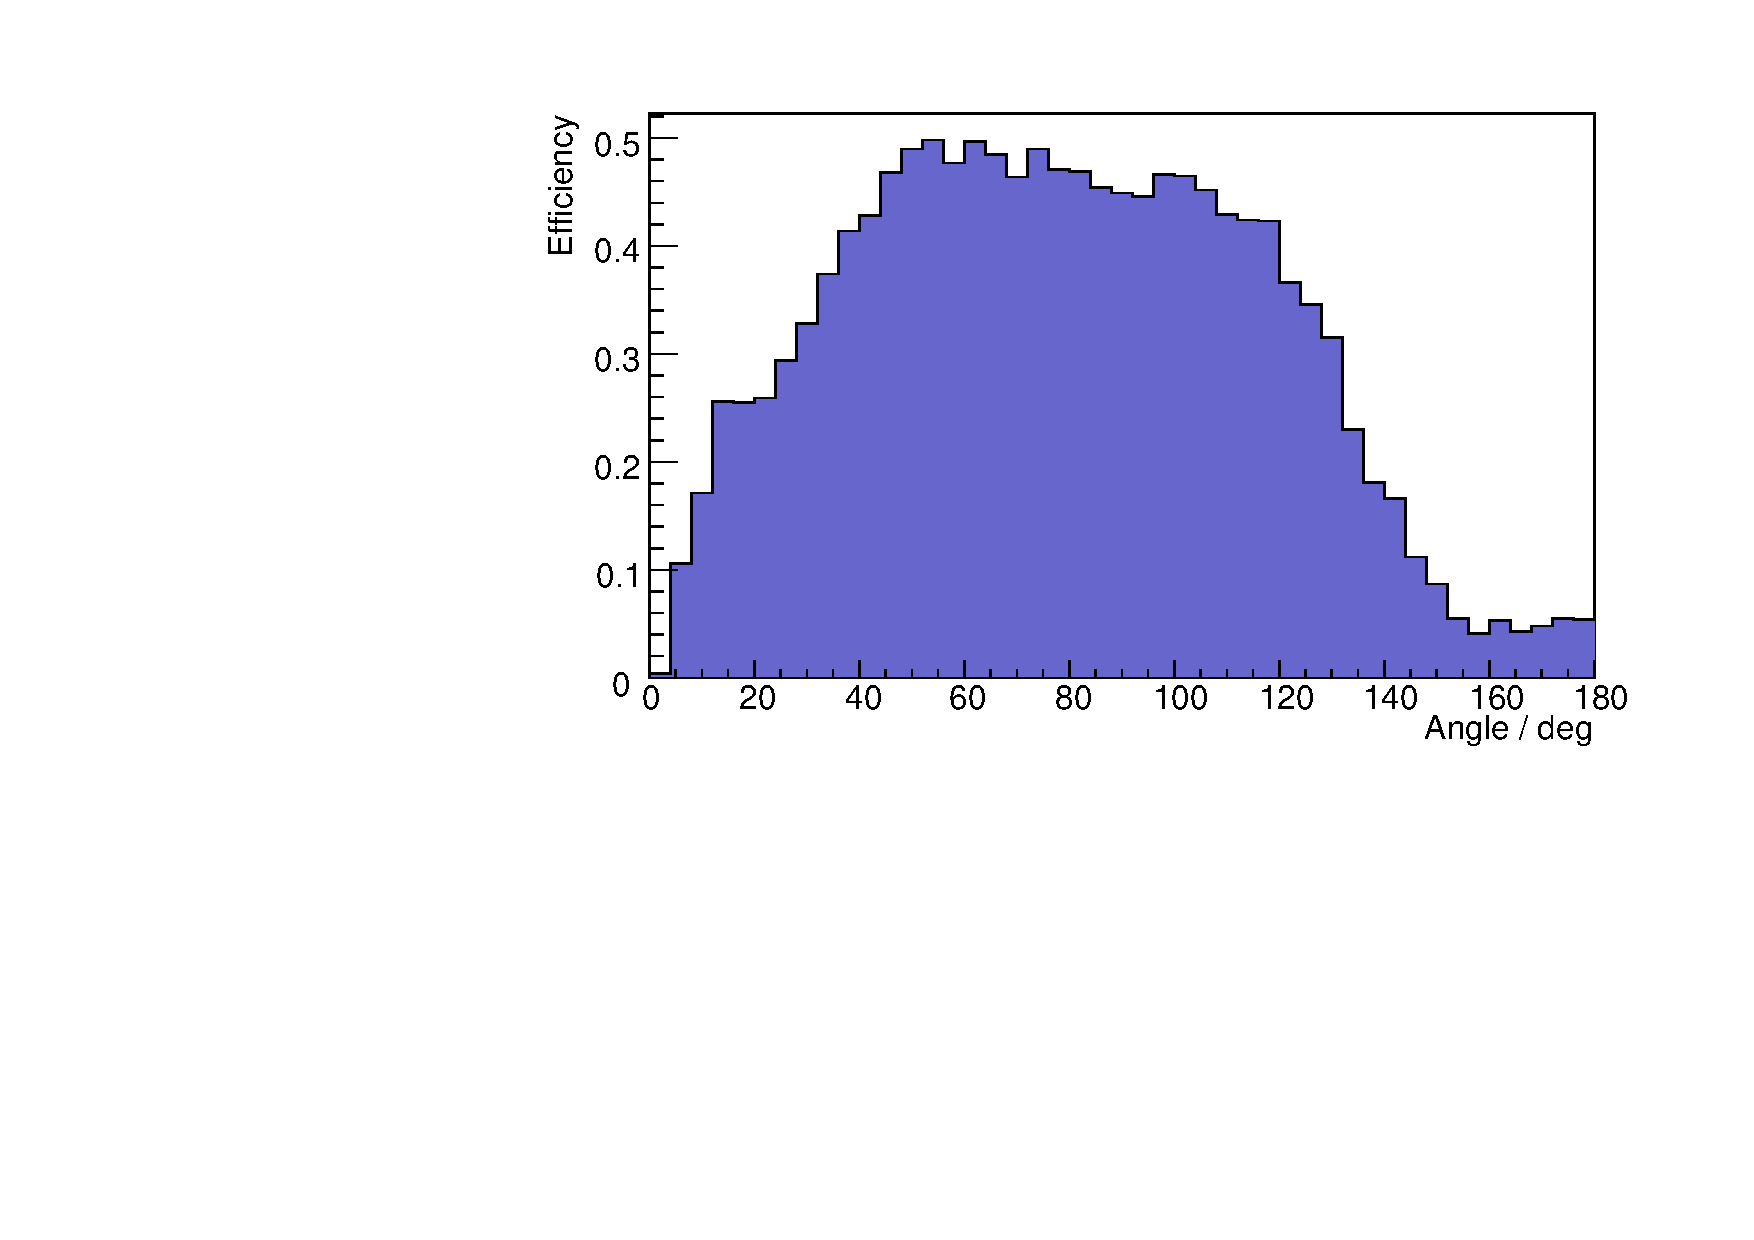
\includegraphics[angle=-90]{chapters/cellularautomaton_images/toy_raw_eff}}
%\caption[Efficiency for finding 2 tracks for raw CA operating on toy MC events]{\label{fig:ca_toy_raw_twotrack_efficiency}Efficiency for finding two tracks in the raw \ac{CA} operating on toy MC events with fixed opening angle, as a function of that angle. The efficiency is low due to the presence of several short track segments as a result of geometric effects in the operation of the \ac{CA}. For the most part these can be merged together. The efficiency drops further for angles above $140\degree$ since the \ac{CA} cannot distinguish such large opening angles from continuous straight line tracks.}
%\end{figure}

While the raw performance of the \ac{CA}, characterised by the efficiency for finding two tracks, is poor, the resultant clustering typically provides long track candidates which can be used as key tracks in the track road merging process. Figure \ref{fig:ca-openingangle-sample-event-raw} shows the raw clusters output by the CA for one such event. Although there are many clusters, one track was successfully identified in its entirety, while the other is split into several shorter segments. Each segment is long enough to act as a seed point from which almost all of the segments may be merged together to recover the other long track. As such, the CA provides a significant advantage over applying a combinatoric approach using only track road algorithms, which is impractical given the large numbers of hits typically associated with a neutrino event in a \ac{LAr TPC}. The segmented track in this event is due to the CA being unable to cope with geometric effects introduced by the voxellised nature of the data. These effects tend to produce runs of linear structures, separated by a jump or step that the CA interprets to be a large angle between cells; one of the criteria for breaking a track in two. This is a natural outcome from the CA and is the desired effect when dealing with vertices and interaction points, so it cannot be ``tuned out''. The merging algorithm discussed below aims to compensate for these cases in which the track structure remains sufficiently linear to suggest that the desired outcome is one cluster, not two.

%% --------------------------------------------------
%% SUBSECTION: Performance of the CA with Merging
%% --------------------------------------------------
\subsection{Performance of the \acl{CA} with Merging}
When the merging process is applied, the track counts (figure \ref{fig:ca_toy_merged_trackcounts}) %and two track efficiency (figure \ref{fig:ca_toy_merged_twotrack_efficiency})
are considerably improved. The merging process tidies the events up, gathering together any track fragments and recombining them with the track they should belong to. In some cases, small track fragments remain, and while the modal number of tracks after merging is $2$, there is a long tail caused by a handful of events with significantly more tracks after merging. A simple range cut can be imposed to remove these remaining fragments.

\begin{figure}
\centering
% "Run8": CA Theta 10 deg, CW Radius 6 mm, Merging radius 5 mm
\resizebox{0.9\textwidth}{!}{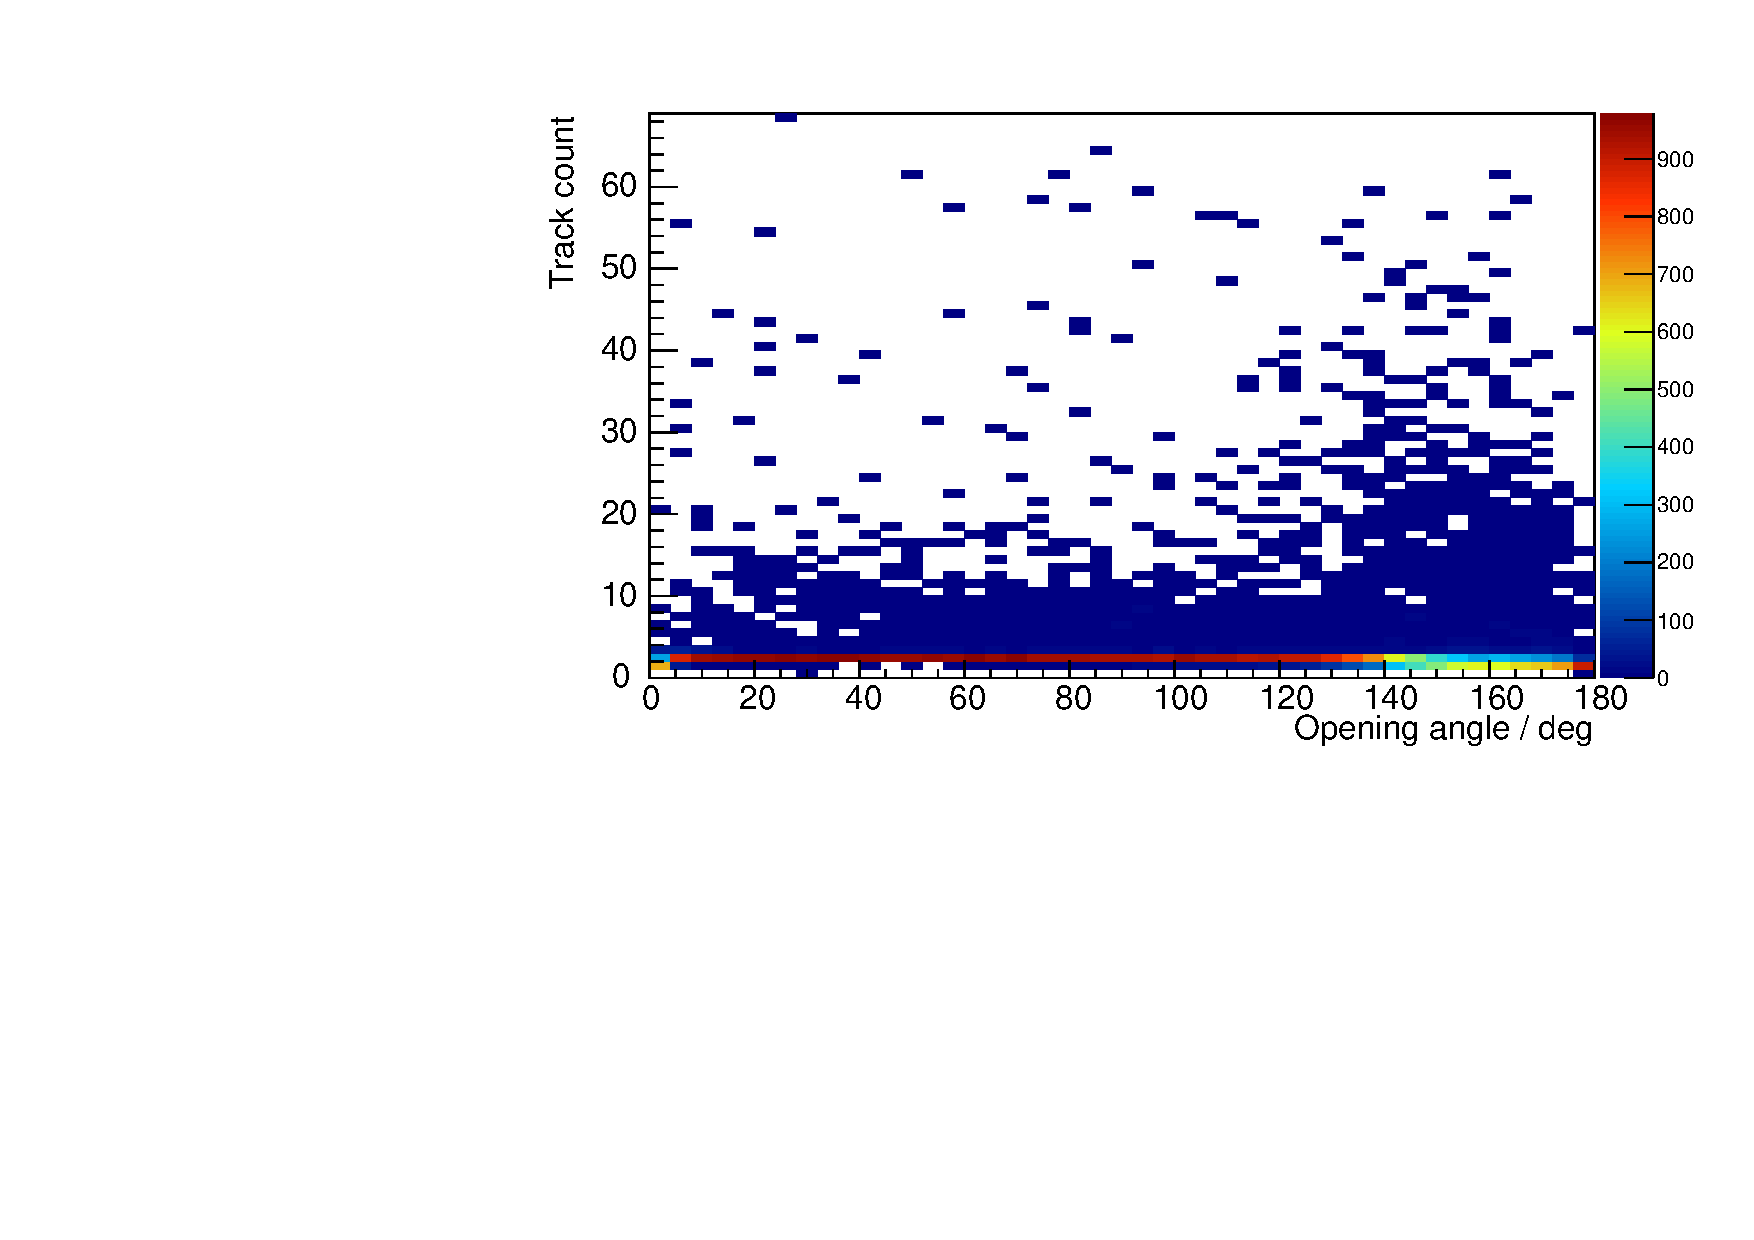
\includegraphics[angle=-90]{chapters/cellularautomaton_images/toy_merged_counts}}
\caption[Track count as a function of angle for CA with merging operating on toy MC events]{\label{fig:ca_toy_merged_trackcounts}Number of tracks found as a function of opening angle for the \ac{CA} with track road merging operating on two track events with a fixed opening angle. There are 1000 events per opening angle, and the events are rotated so as to be distributed isotropically. A small track fragment is usually left over, which can be removed with a suitable range cut.}
\end{figure}

%\begin{figure}
%\centering
%\resizebox{0.9\textwidth}{!}{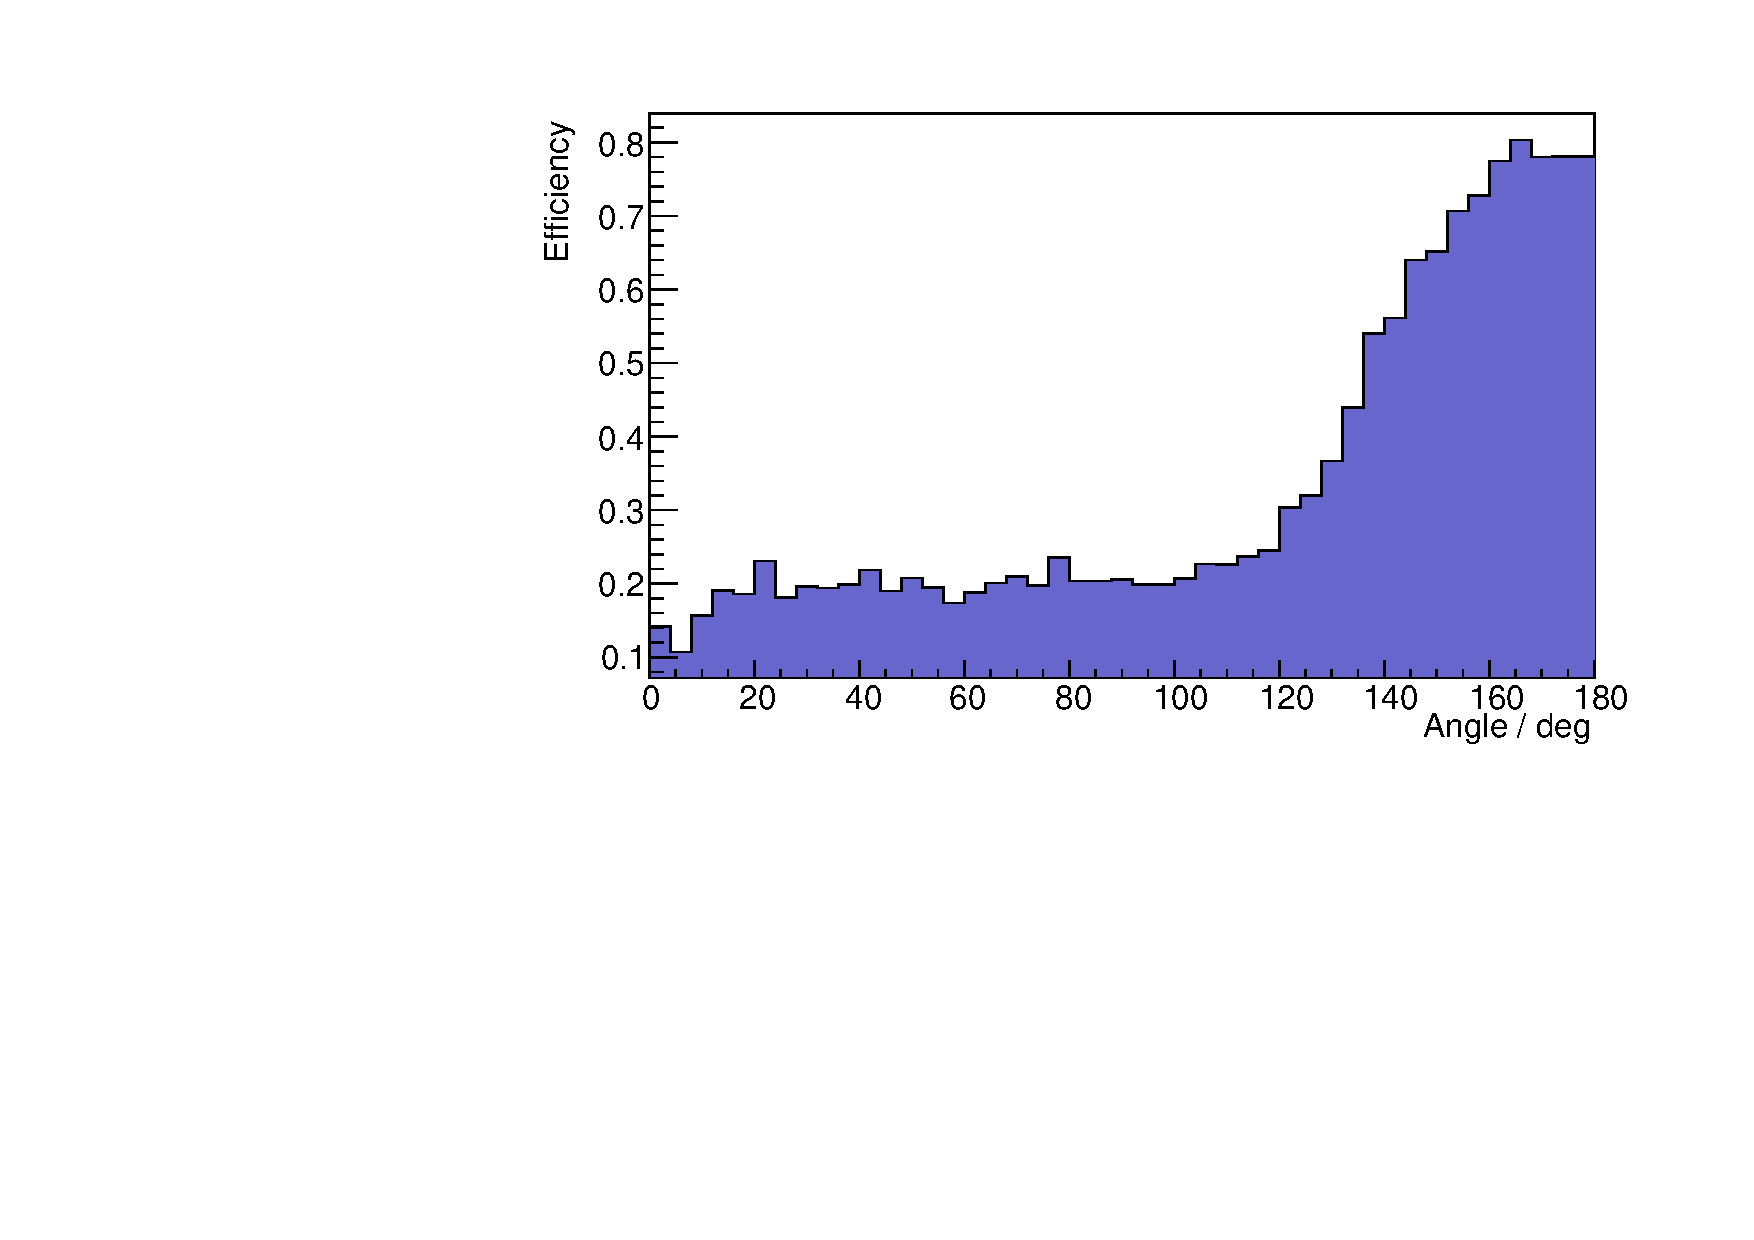
\includegraphics[angle=-90]{chapters/cellularautomaton_images/toy_merged_eff}}
%\caption[Efficiency for finding 2 tracks for CA with merging operating on toy MC events]{\label{fig:ca_toy_merged_twotrack_efficiency}Efficiency for finding two tracks in the \ac{CA} with track road merging operating on toy MC events with fixed opening angle, as a function of that angle. The efficiency is low due to small remnant fragments, which can be removed with a suitable range cut.}
%\end{figure}

%% --------------------------------------------------
%% SUBSECTION: Performance after a range cut
%% --------------------------------------------------
\subsection{Performance After a Range Cut}
After imposing a range cut of 20 hits (corresponding roughly to $20\mm$ or $4.2\MeV$ deposited by a minimum-ionising particle) the performance improves further. Now, the mean number of tracks (see figure \ref{fig:ca_toy_rcut_trackcounts}) is 2, giving a high two track reconstruction efficiency (figure \ref{fig:ca_toy_rcut_twotrack_efficiency}) for most opening angles. Above an opening angle of about $140\degree$ the \ac{CA} fails to cluster the two lines separately since the change in angle from one line to the next is now small and the \ac{CA} can smoothly travel across the join, resulting in a single output cluster. This is not symmetric with the case at an opening angle of $40\degree$, where the angle between the tracks is much sharper, and the \ac{CA} can easily distinguish the two. Efficiency curves are shown in fig. \ref{fig:ca_toy_rcut_twotrack_efficiency} at four different purity levels, defined on a hit level as the fraction of hits in a cluster which came from the same truth track. At $80\%$ and $85\%$ purity, the \ac{CA} performs with a high efficiency. This is reduced slightly for a requirement of $90\%$ purity, and substantially for a requirement of $95\%$ purity. The \ac{CA} can therefore be said to cluster simple topologies with very high efficiency and with reasonable purity, up to geometric opening angles of $140\degree$.

\begin{figure}
\centering
\resizebox{0.9\textwidth}{!}{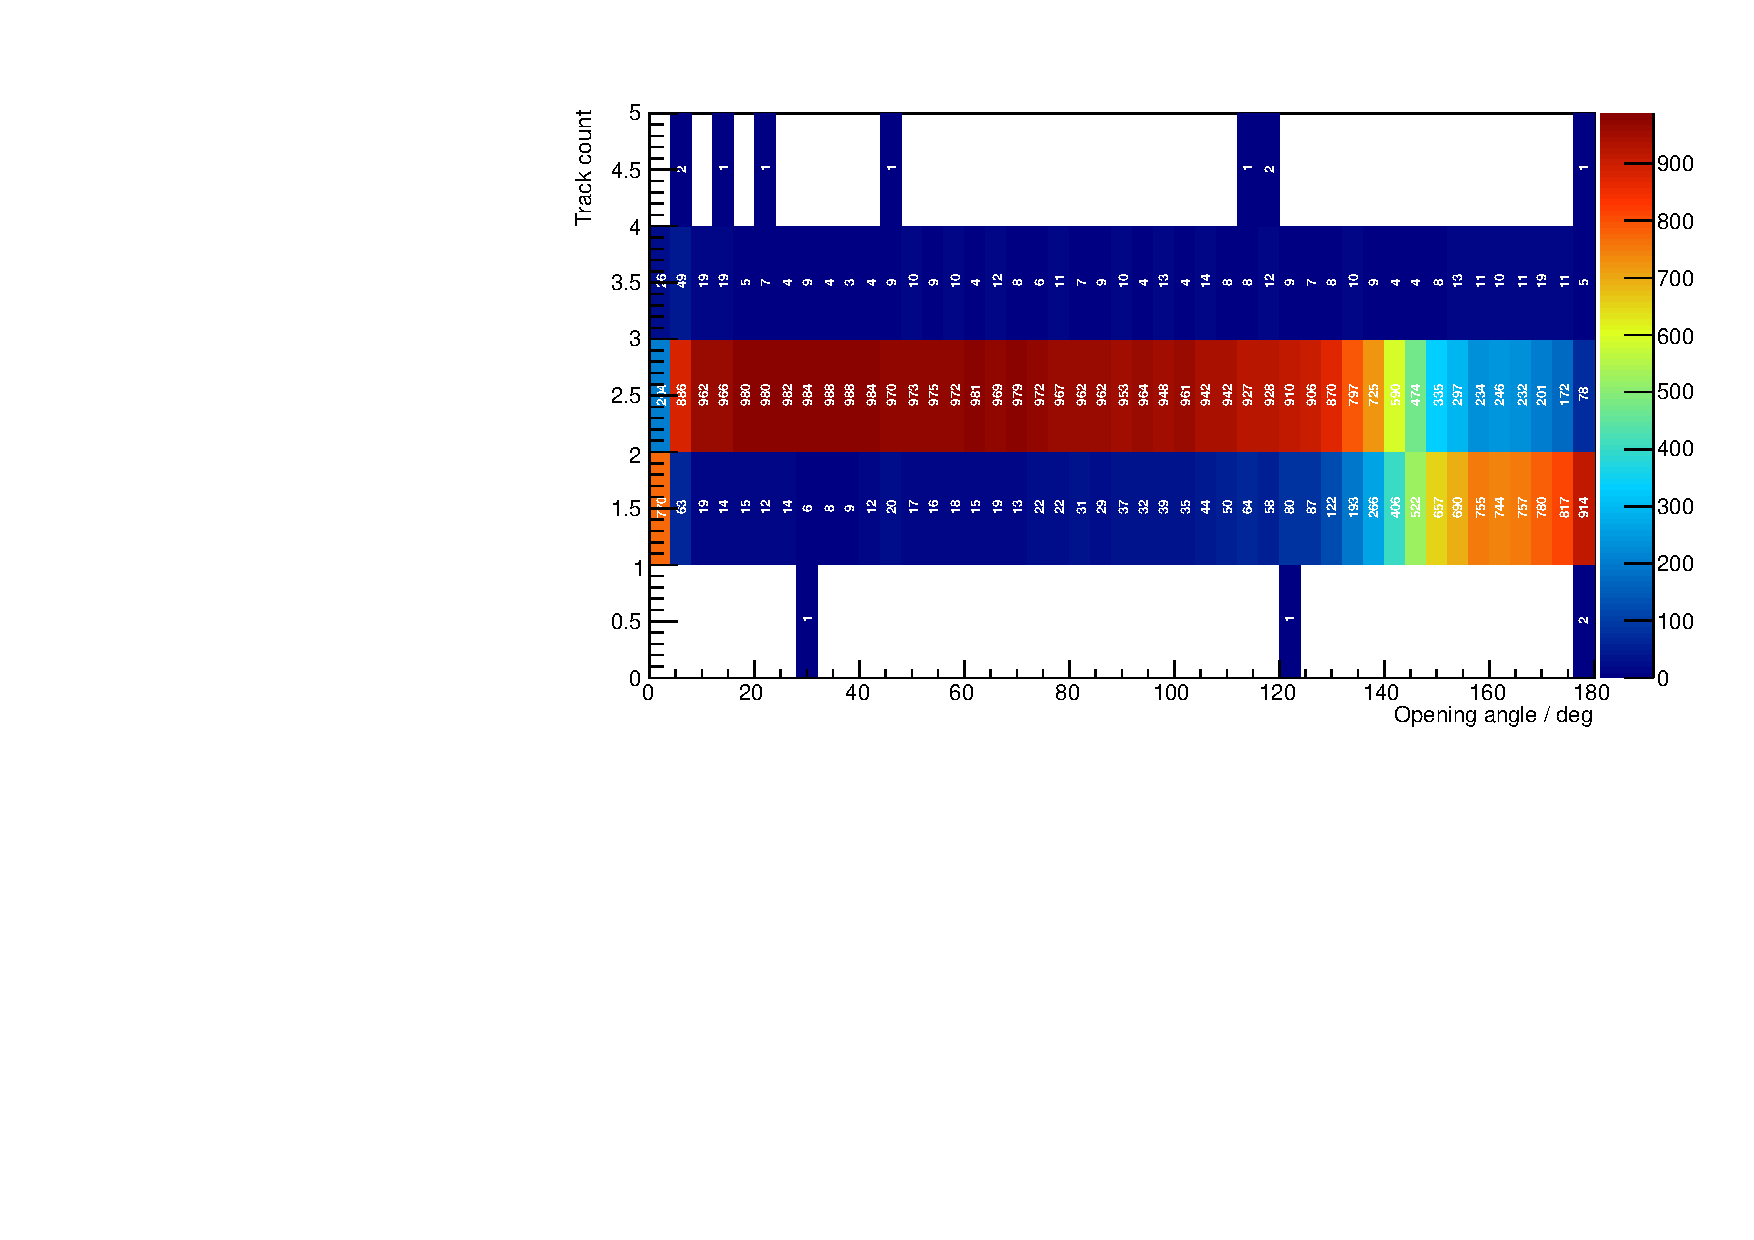
\includegraphics[angle=-90]{chapters/cellularautomaton_images/toy_rcut_counts}}
\caption[Track count as a function of angle for CA with merging and range cut operating on toy MC events]{\label{fig:ca_toy_rcut_trackcounts}Number of tracks found as a function of opening angle for the \ac{CA} with track road merging operating and a range cut of $20\mm$ on two track events with a fixed opening angle. There are 1000 events per opening angle, and the events are rotated so as to be distributed isotropically. The mean number of tracks found is now 2, dropping to 1 above $140\degree$ due to an inability of the \ac{CA} to distinguish this topology from that of a single continuous line.}
\end{figure}

\begin{figure}
\centering
\resizebox{0.9\textwidth}{!}{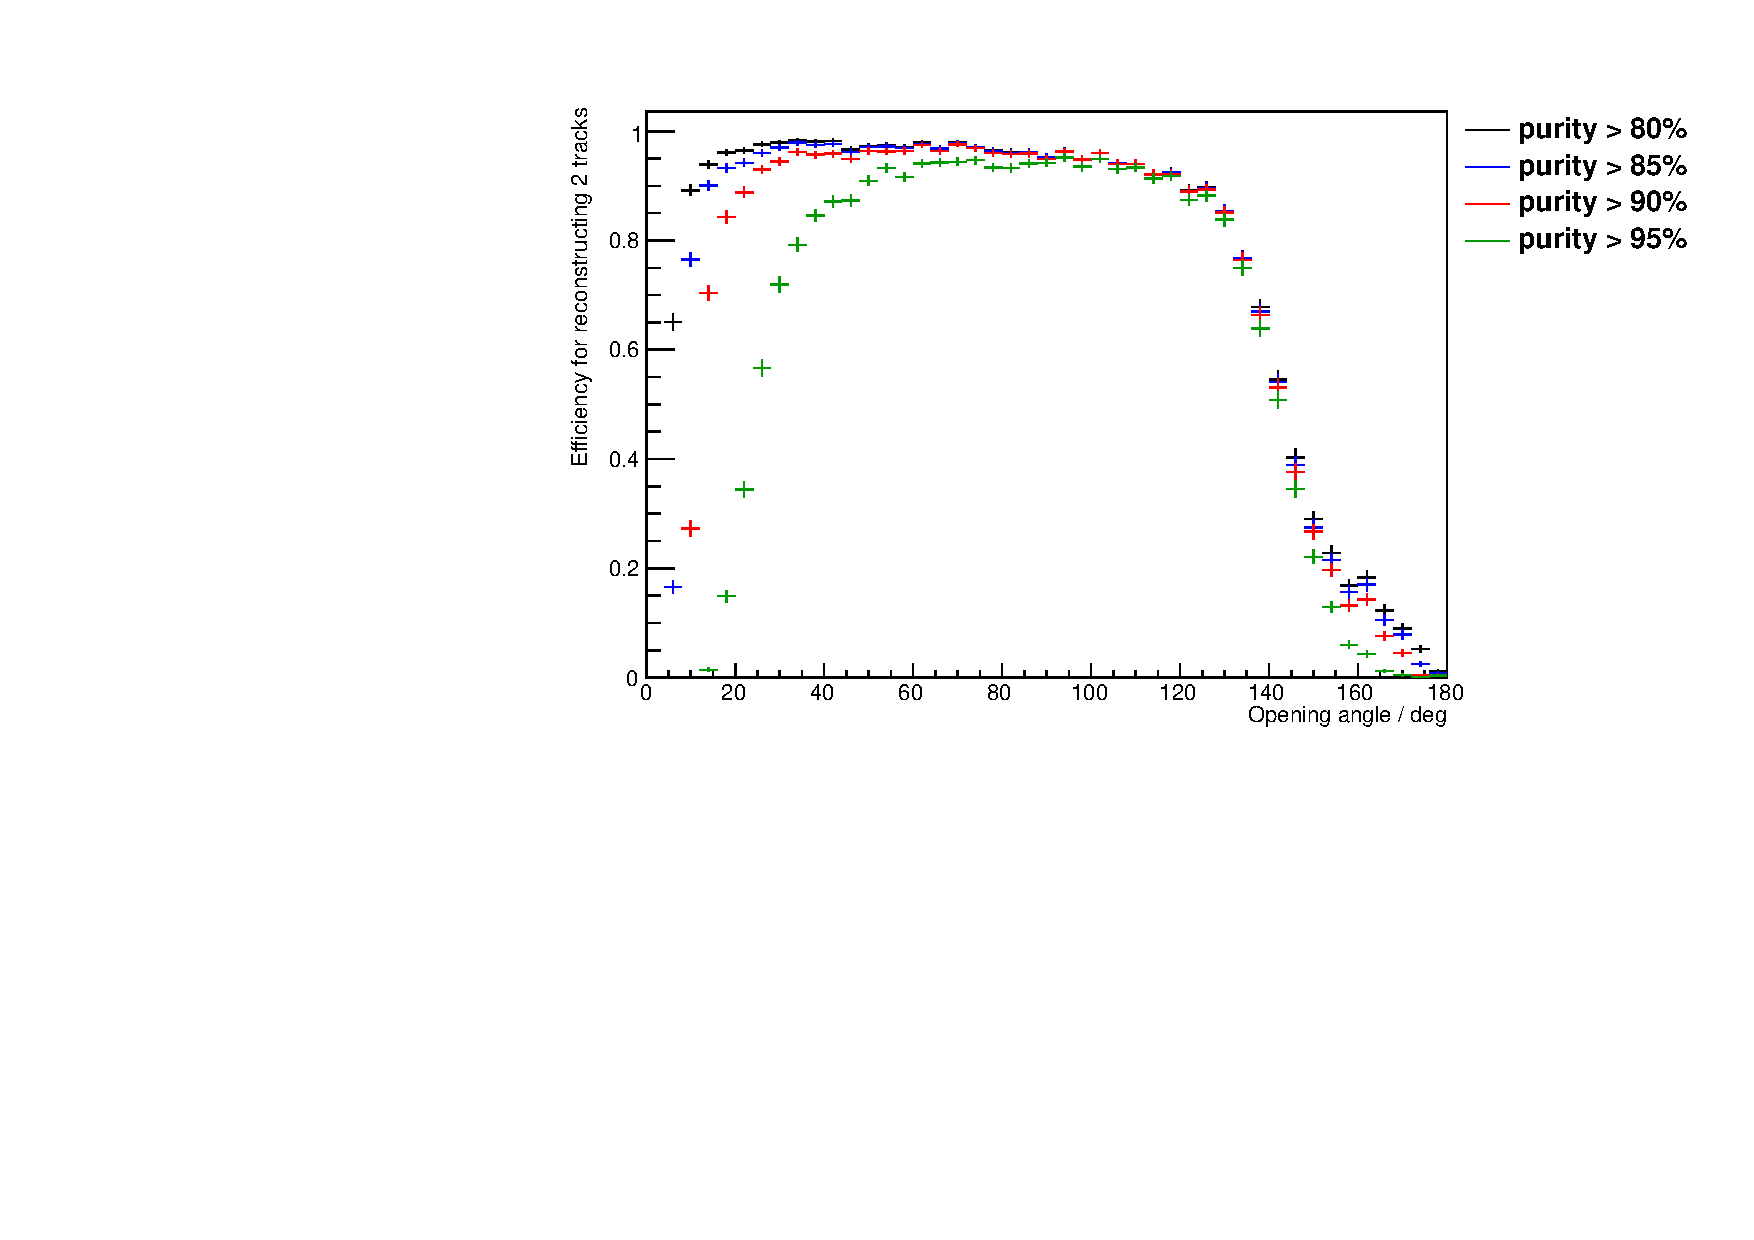
\includegraphics[angle=-90]{chapters/cellularautomaton_images/toy_rcut_eff}}
\caption[Efficiency for finding 2 tracks for CA with merging and range cut operating on toy MC events]{\label{fig:ca_toy_rcut_twotrack_efficiency}Efficiency for finding two tracks in the \ac{CA} with track road merging and a range cut of $20\mm$ operating on toy MC events with fixed opening angle, as a function of opening angle. Efficiency curves are plotted for four different purity cuts, requiring a minimum of $80\%$ (black), $85\%$ (blue), $90\%$ (red) and $95\%$ (green) purity in each track. The efficiency is high for almost all angles up to $140\degree$, beyond which the \ac{CA} is unable to distinguish the topology from that of a single continuous track.}
\end{figure}


\clearpage
%% --------------------------------------------------
%% SUBSECTION: Performance of the CA on Genie MC Events
%% --------------------------------------------------
\section{Performance of the \acl{CA} on Genie Monte Carlo Events}
The data for this section consists of neutrino events generated using Genie and tracked through a detector using Geant4, as described in chapters \ref{sec:genie} and \ref{sec:lamu} respectively. The reconstruction algorithm is applied first to charged current $\nu_\mu$ interactions producing $\ccqe$ final states (often referred to as \acl{CCQE} events), and then to charged current $\nu_\mu$ interactions producing $\ccpi$ final states.

\subsection{Charged Current $\nu_\mu \rightarrow \ccqe$ (CCQE)}
The Genie event generator was used to model the interactions of $0.77\GeV$ muon neutrinos on Argon nuclei. A sample was obtained of 1000 charged current interactions resulting in $\ccqe$ (only) final states. The resulting events were tracked through a liquid Argon TPC using Geant4 and the voxel data stored for analysis. Interactions of this type are of particular interest because they account for approximately 66\% of the interaction cross section at low energy and the two-body final state allows an accurate estimate of the muon neutrino energy to be made from the muon kinematics alone.

This data sample raises the possibility of attempting to optimise the \ac{CA} parameters for reconstructing neutrino events. Since it is a full simulation, the events will contain noise arising from delta electrons, hadronic reinteraction of the proton, muon decay and other physics processes. The truth information recorded for each event allows for the selection of a subset of this information, for example just the hits corresponding to energy deposited by the primary particles. In this way it is possible to optimise the algorithms based on more realistic data than in the toy study, but without including obviously difficult events.

\subsubsection{Long Two-Track Events}
In the first instance, events were selected in which both the proton and muon contained over 200 hits (corresponding approximately to a $20\cm$ straight line) and the hits from other particles were stripped from the event prior to running the \ac{CA}. The resulting events therefore contain two long tracks and nothing else. In a small number of cases, the event topology may make it difficult for the \ac{CA} to reconstruct these events correctly, e.g. if the muon and proton were produced almost back-to-back, or if either particle undergoes a large scatter along its trajectory, but for the most part these events should be reconstructed with two clusters in the \ac{CA} output.

A total of 483 events out of the sample of 1000 contain muon and proton tracks with over 200 hits each. Three parameters available in the reconstruction algorithms were varied and these 483 events processed with each permutation. The parameters are the \ac{CA} track angle $\theta$ ($10\degree$, $20\degree$ and $30\degree$), the charge weighting radius $R_{w}$ ($2.0\mm$, $5.0\mm$ and $10.0\mm$) and the track merging radius $R_m$ ($10\mm$, $20\mm$ and $30\mm$). The results of this optimisation are shown in table \ref{table:ccqe-2tr-opt-results}, which lists the number of events reconstructed with one, two or three tracks against the reconstruction parameters used. The results are sorted by the number of events reconstructed with two tracks. The largest number of two-track events are returned from the algorithm when used with parameters $\theta=10.0\degree$, $R_w=5.0\mm$ and $R_m=30.0\mm$. These parameters yield 345 two-track events, corresponding to $71.4\%$ of the input sample. In addition, these parameters give a low number of one- and three-track events.

\begin{table}
\centering
\begin{tabular}{*{6}{r}}
$\theta$ ($\degree$) & $R_w$ ($\mm$) & $R_m$ ($\mm$) & $\phantom{000} $$N_1$  & $\phantom{000}$ $N_2$  & $\phantom{000}$ $N_3$  \\
\hline
\hline
10.0  & 5.0   & 30.0  & 59   & 345  & 72 \\
10.0  & 5.0   & 20.0  & 43   & 341  & 84 \\
10.0  & 10.0  & 30.0  & 91   & 335  & 53 \\
10.0  & 5.0   & 10.0  & 35   & 331  & 70 \\
10.0  & 10.0  & 20.0  & 76   & 331  & 66 \\
10.0  & 10.0  & 10.0  & 67   & 327  & 62 \\
20.0  & 5.0   & 30.0  & 109  & 305  & 62 \\
20.0  & 5.0   & 20.0  & 94   & 305  & 70 \\
20.0  & 2.0   & 30.0  & 64   & 302  & 109 \\
20.0  & 5.0   & 10.0  & 85   & 301  & 55 \\
20.0  & 2.0   & 20.0  & 49   & 301  & 114 \\
20.0  & 2.0   & 10.0  & 38   & 293  & 98 \\
30.0  & 2.0   & 30.0  & 101  & 288  & 87 \\
30.0  & 2.0   & 20.0  & 88   & 288  & 89 \\
30.0  & 2.0   & 10.0  & 79   & 279  & 77 \\
20.0  & 10.0  & 30.0  & 196  & 237  & 46 \\
20.0  & 10.0  & 20.0  & 189  & 231  & 53 \\
20.0  & 10.0  & 10.0  & 188  & 217  & 56 \\
30.0  & 5.0   & 30.0  & 206  & 210  & 59 \\
30.0  & 5.0   & 20.0  & 198  & 204  & 67 \\
30.0  & 5.0   & 10.0  & 195  & 195  & 55 \\
10.0  & 2.0   & 30.0  & 28   & 170  & 246 \\
30.0  & 10.0  & 30.0  & 276  & 163  & 40 \\
30.0  & 10.0  & 20.0  & 271  & 157  & 45 \\
30.0  & 10.0  & 10.0  & 271  & 143  & 50 \\
10.0  & 2.0   & 20.0  & 16   & 97   & 285 \\
10.0  & 2.0   & 10.0  & 4    & 56   & 189 \\
\hline
\end{tabular}
\caption[Optimisation of Cellular Automaton reconstruction parameters]{\label{table:ccqe-2tr-opt-results}Optimisation of reconstruction parameters in the \ac{CA} for reduced CCQE events (see text for details). Data is shown for the number of events reconstructed as containing one, two or three tracks ($N_1$, $N_2$ and $N_3$) for different combinations of the track opening angle $\theta$, the charge weighting radius $R_w$ and the track merging radius $R_m$. Entries are sorted by the number of events reconstructed with two tracks ($N_2$), largest first. Each set of parameters was used to process the same 483 events. Events with more than three reconstructed tracks are not shown.}
\end{table}

While the number of tracks found in an event is one metric of the quality of the reconstruction, it is also important to consider \emph{hit efficiencies} and \emph{track purities}.
\begin{description}
    \item[Hit efficiency:] A measure of how much of the original event data is retained. Hits that are present in any output cluster, divided by the number of input hits. High hit efficiency means that the algorithm is not throwing away many hits, which makes subsequent energy calculations easier. Due to the nature of the \ac{CA}, the algorithm will necessarily throw away some hits but the track structures should remain and lost hits can be retrieved with track-road style merging applied to the original data, rather than to a cluster, if required.
    \item[Track purity:] A measure of how selective the clustering is. An output cluster will contain hits from one or more truth tracks. The track purity is the largest number of contributing hits from a single track, divided by the total number of hits. High purity means that the \ac{CA} clustered mostly hits from a single trajectory together. This is extremely important, though the purity is often diluted by hits from e.g. delta electrons produced along the length of a muon track, but clustered with it.
\end{description}

Figure \ref{fig:ca-ccqe-reduced-eff-pur-efficiency} shows the hit efficiency and figure \ref{fig:ca-ccqe-reduced-eff-pur-purity} track purity results from the analysis performed with $\theta=10\degree$, $R_w=5.0\mm$ and $R_m=30.0\mm$. The efficiency drops slightly with track length, most likely due to increased scattering as the particle that produced the track loses energy and slows down. The \ac{CA} will struggle with situations where the scattering angles exceed the track breaking angle $\theta$, and will produce many short track segments, each of which will be filtered out in subsequent stages unless they can be merged together. The track purity remains over $90\%$ for all track lengths, indicating that the \ac{CA} with these parameters is capable of differentiating extremely well between unrelated trajectories.

\begin{figure}
    \centering
    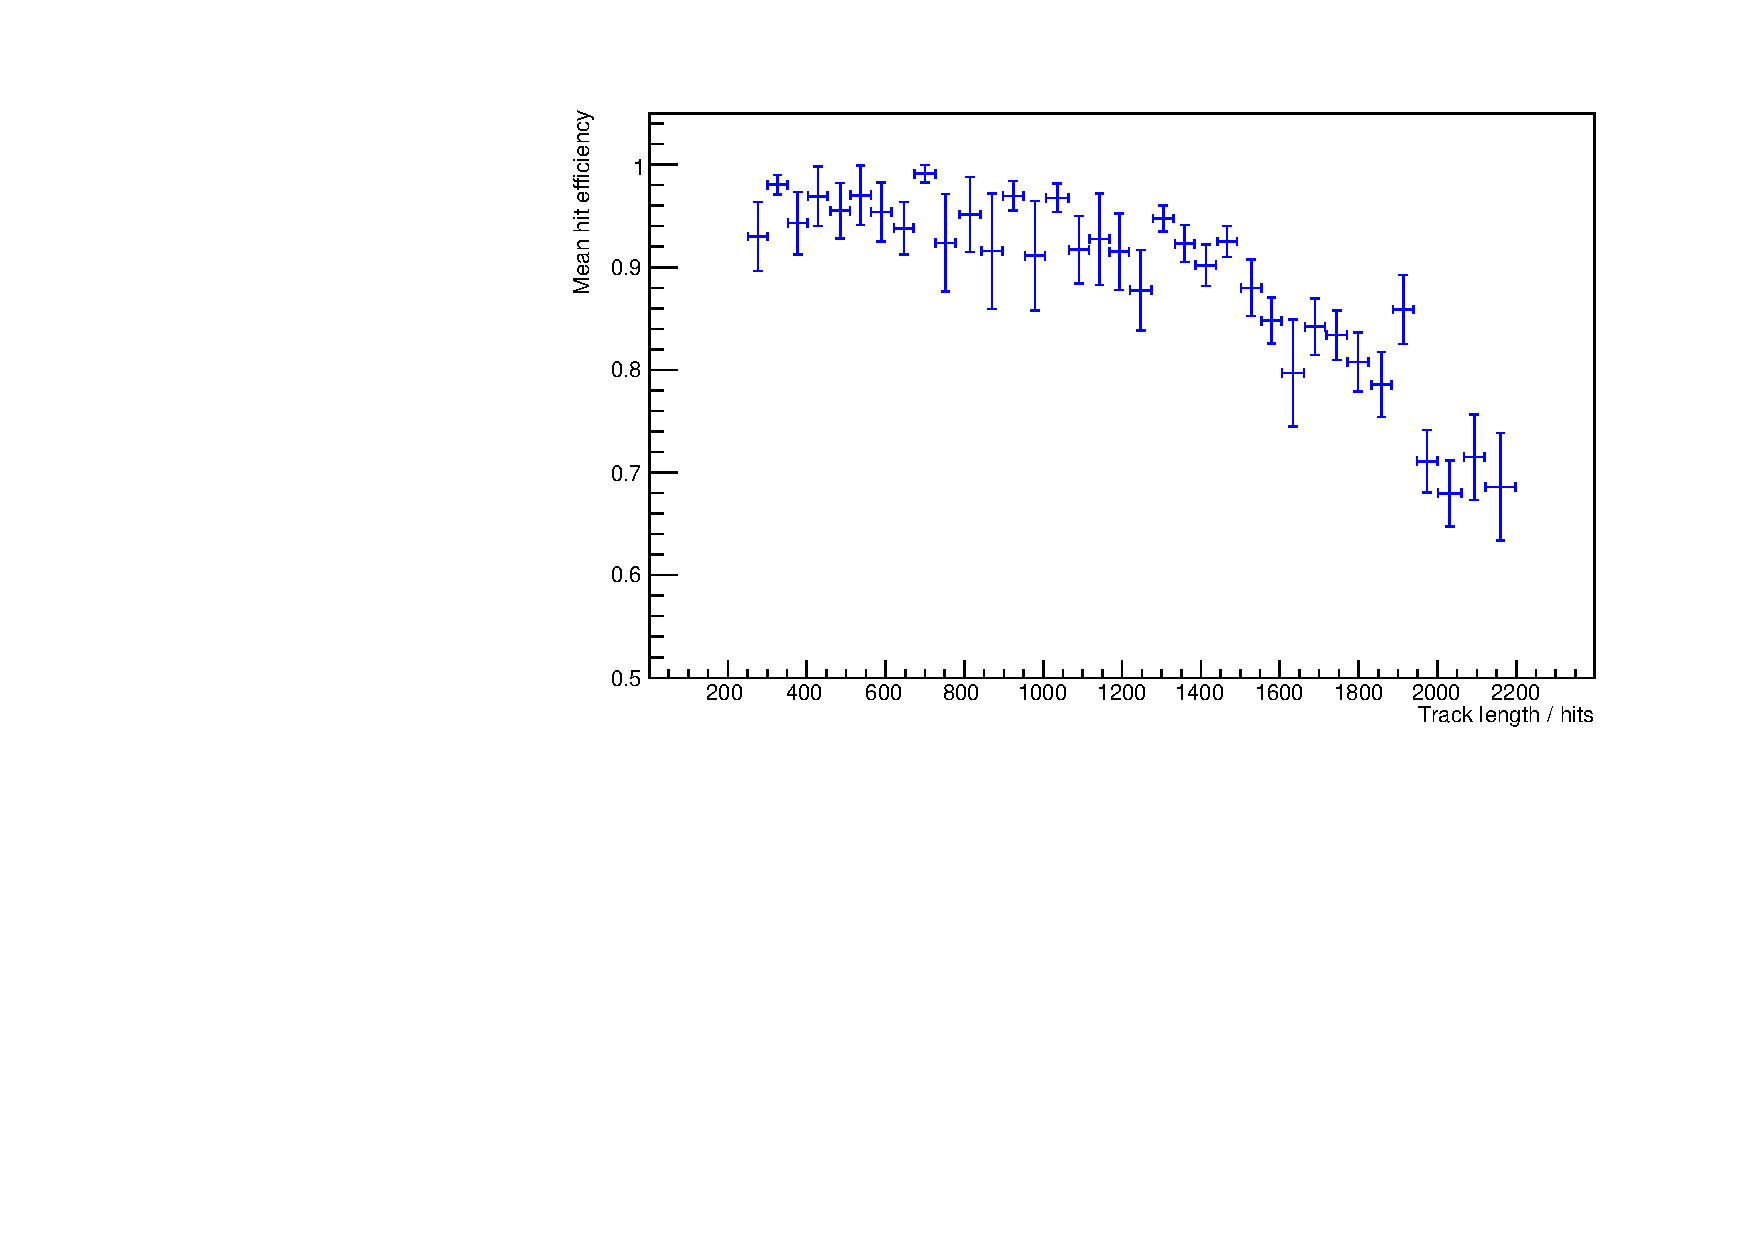
\includegraphics[angle=-90,width=0.8\textwidth]{chapters/cellularautomaton_images/ccqe-reduced-hit-efficiency}
    \caption[Hit efficiency for CA operating on long muon and proton tracks]{\label{fig:ca-ccqe-reduced-eff-pur-efficiency}Hit efficiency for the \ac{CA} operating on long muon and proton tracks from CCQE events. The hit efficiency is high, but drops as a function of track length, indicating that the \ac{CA} is not capable of retaining all hits for long tracks, most likely due to increased scattering.}
\end{figure}

\begin{figure}
    \centering
    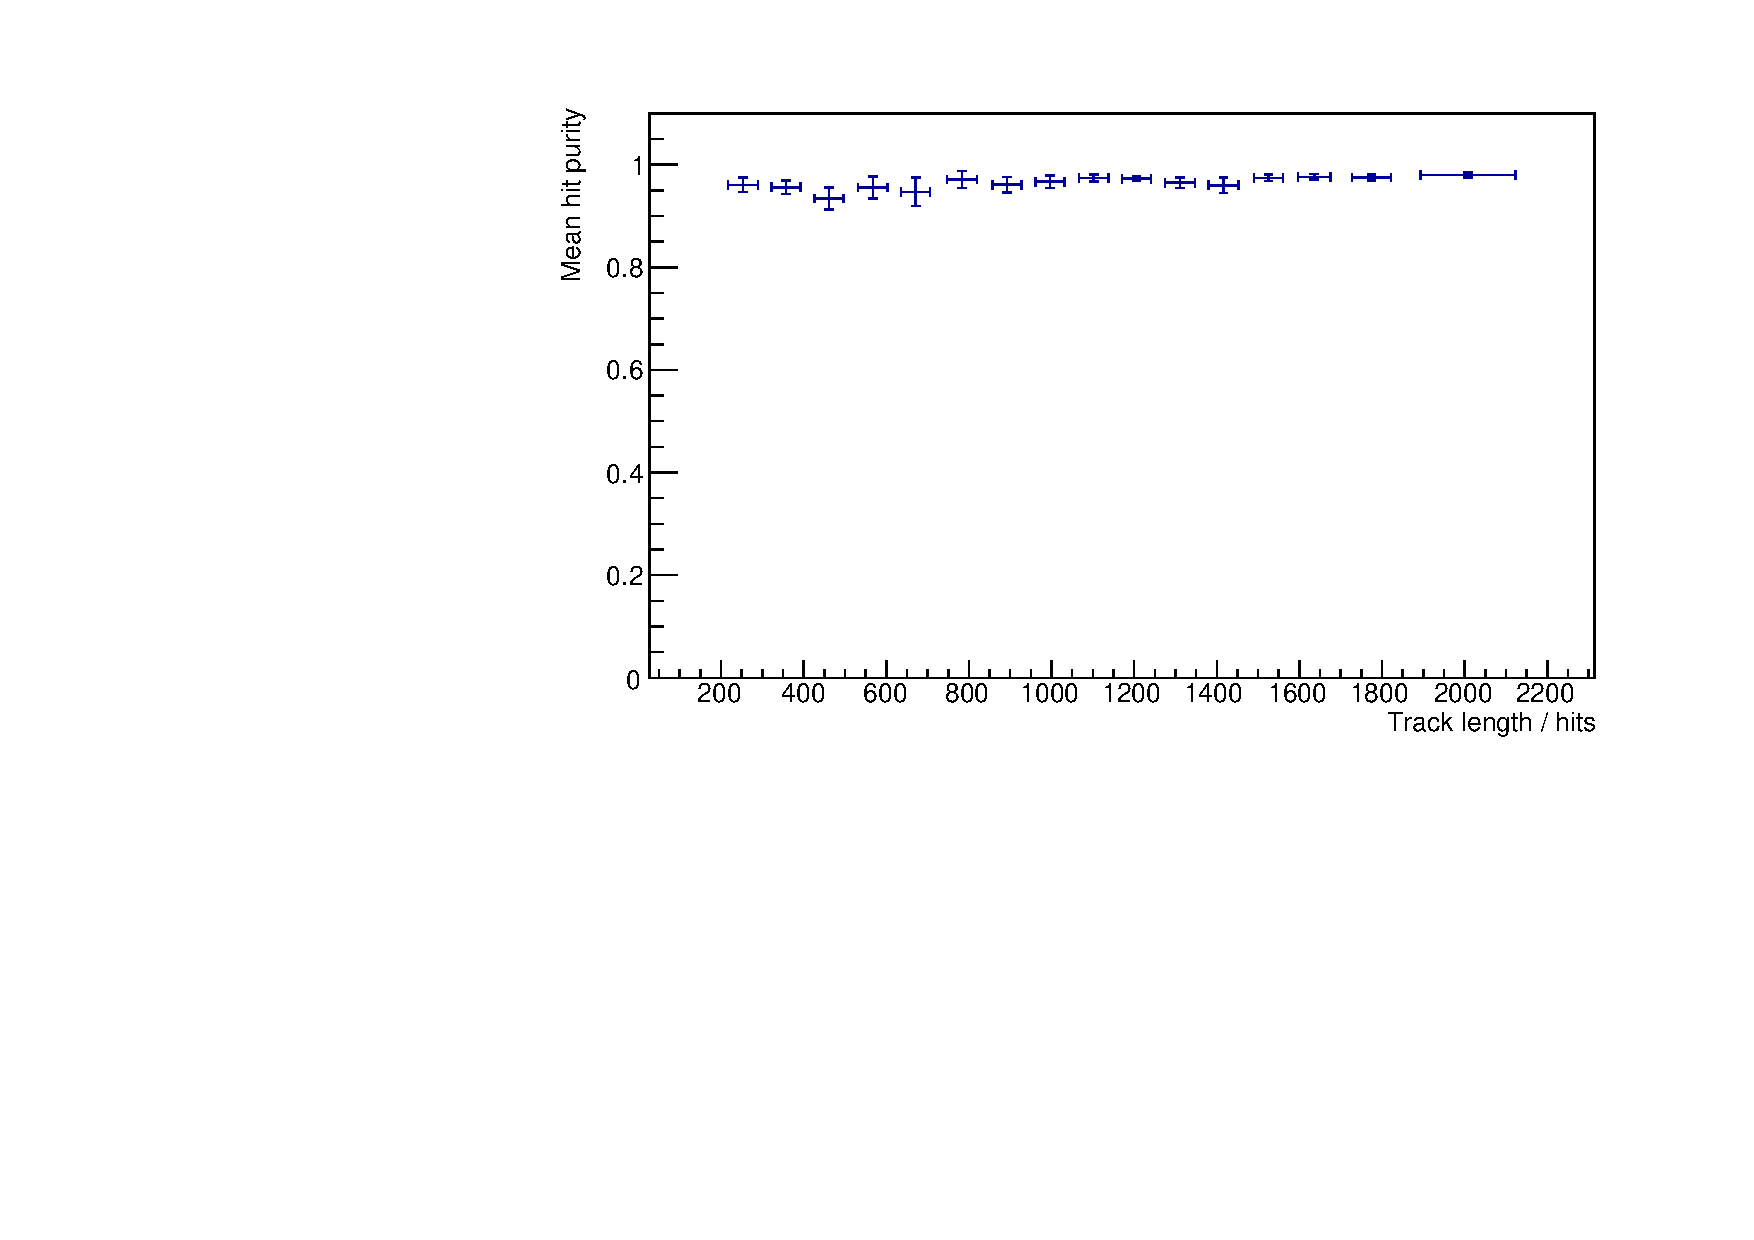
\includegraphics[angle=-90,width=0.8\textwidth]{chapters/cellularautomaton_images/ccqe-reduced-cluster-purity}
    \caption[Track purity for CA operating on long muon and proton tracks]{\label{fig:ca-ccqe-reduced-eff-pur-purity}Track purity for the \ac{CA} operating on long muon and proton tracks from CCQE events. The purity is over $90\%$ for all track lengths, indicating that the \ac{CA} is capable of separating hits resulting from different particles extremely well.}
\end{figure}

\subsubsection{Full Reconstruction}
Having attempted to optimise the parameters on a reduced dataset where two reconstructed tracks are expected, the performance of the \ac{CA} can be assessed when run against the full simulated events. Here, a much smaller range cut of 20 hits is applied. Events containing proton tracks with fewer than 20 hits are not processed, and in the remaining events all objects with fewer than 20 hits are cut out of the data before reconstruction. A 20 hit track corresponds approximately to a $20\mm$ trajectory, or an energy deposit of $4.2\MeV$, based on a minimum-ionising particle depositing $2.1\MeV \cm^{-1}$. Such values can be considered as realistic energy thresholds in any liquid Argon TPC, and the presence of tracks in the simulated data with such short range adds noise that would simply not be seen in a real detector. Following the 20 hit range requirement on protons, 878 events of the 1000 event sample survive for reconstruction. 

Because of this relaxation of the initial range cuts, and because the full event data is now included, the results are expected to be poorer than those for the case presented above. In particular, the noise introduced by delta electrons will serve to pull the \ac{CA} off course as it follows long tracks, and the decay products may themselves contribute additional tracks which can be reconstructed. We should not, therefore, expect the mean number of reconstructed tracks to be two.

Figure \ref{fig:ca-ccqe-full-trackcounts} shows the distribution of reconstructed track counts. Of the 878 events, 420 ($47.8\%$) had two reconstructed tracks, while a further 270 ($30\%$) had three reconstructed tracks and a further 86 events ($9.7\%$) had four or more reconstructed tracks. The maximum number of reconstructed tracks was six, which occurred for only three events. Given the full set of data included, these numbers are within expectation, i.e. almost $80\%$ of the events have two or three tracks, corresponding most likely to the proton, muon and either a delta or Michel electron. Those events with four or more reconstructed tracks bring the total to almost $90\%$, leaving 102 events ($11.6\%$) reconstructed with just one track.

The relatively large number of events reconstructed with just one track can be put down to a number of geometric effects in the interaction topologies, including short proton tracks running along almost the same trajectory as the muon, or proton tracks at large angles to the muon. It was already demonstrated in section \ref{sec:ca-toy-tracks} that the \ac{CA} cannot cope with extremely large opening angles (greater than about $140\degree$). Figure \ref{fig:ca-clusters-ccqe} shows the output from the CA for three events from this sample, with clusters indicated by colour.

\begin{figure}
    \centering
    \subfigure[]{
        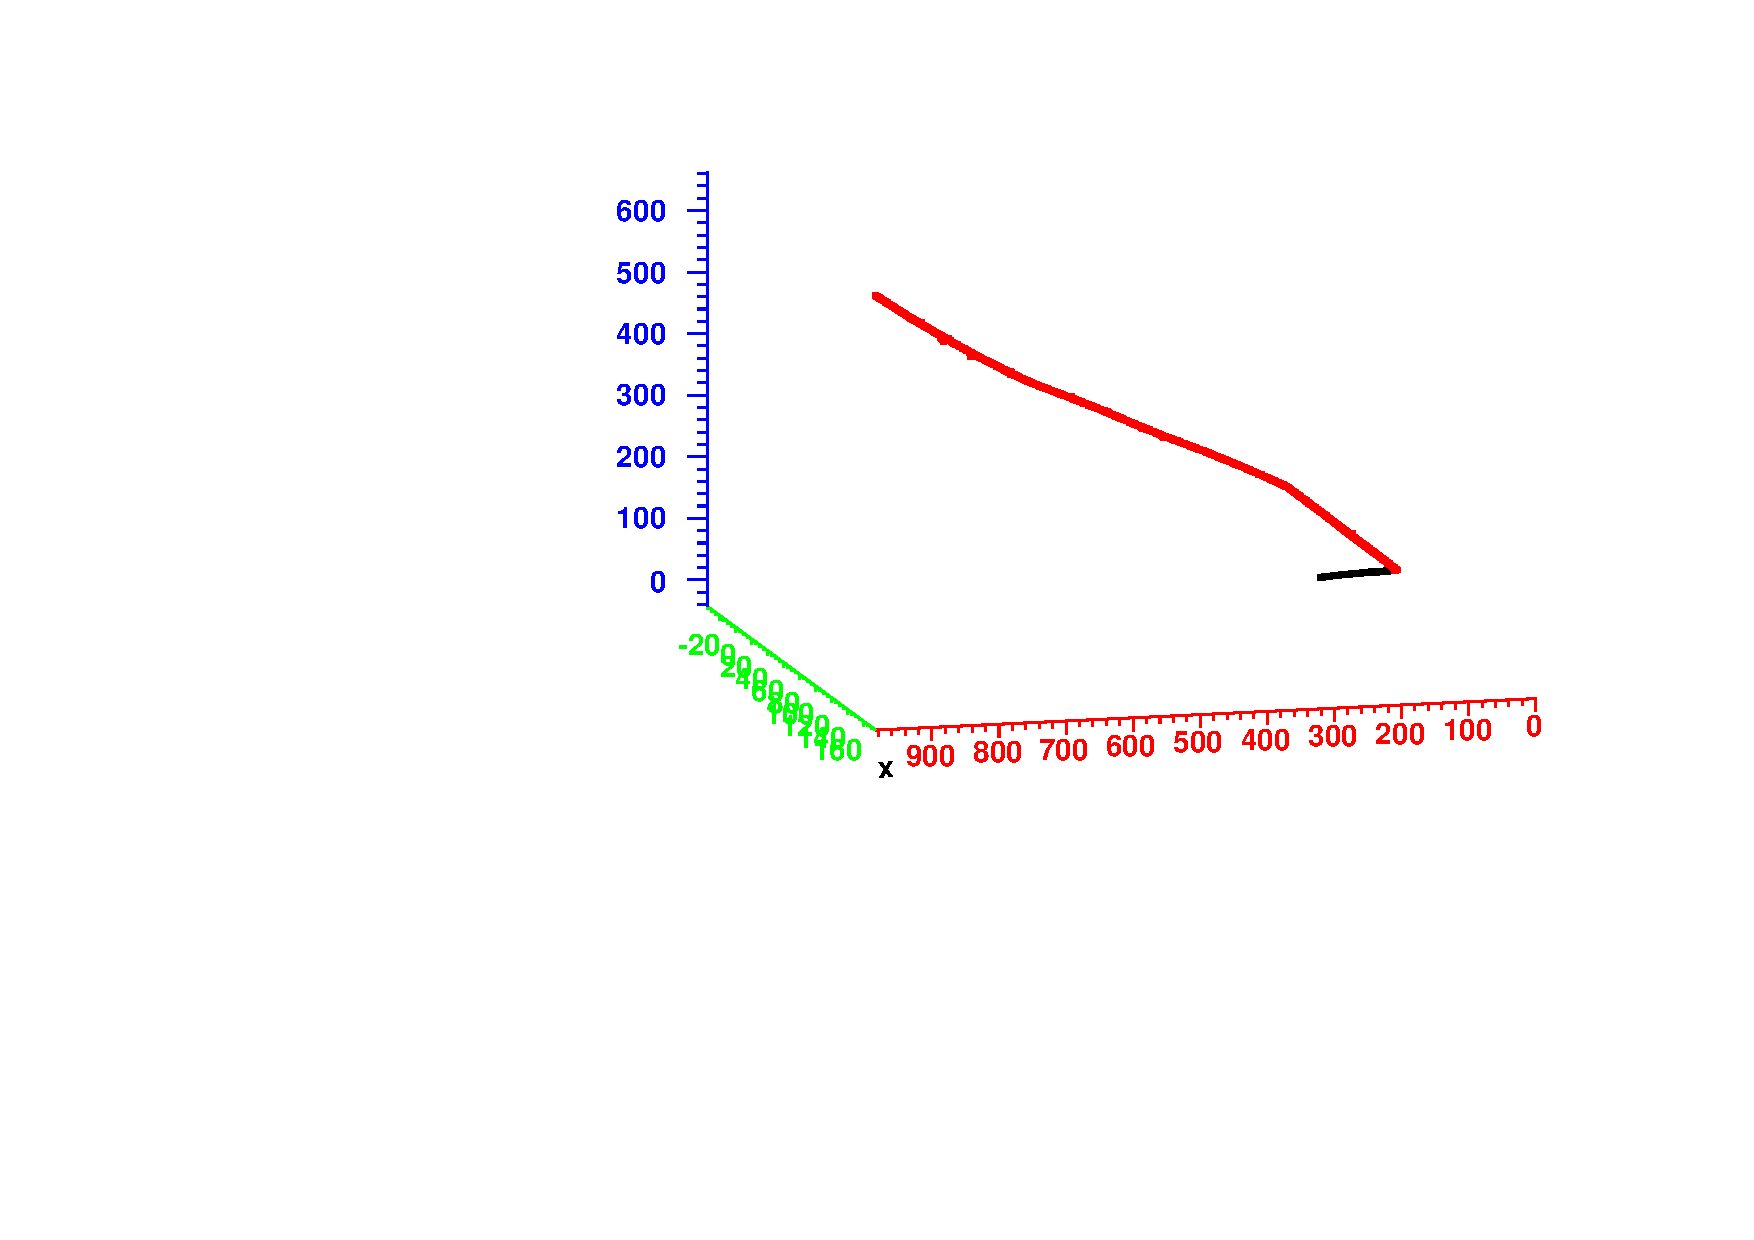
\includegraphics[angle=-90,width=0.6\textwidth]{chapters/cellularautomaton_images/event_8_2tr}
        \label{fig:ca-clusters-ccqe-2tr}
    }
    \subfigure[]{
        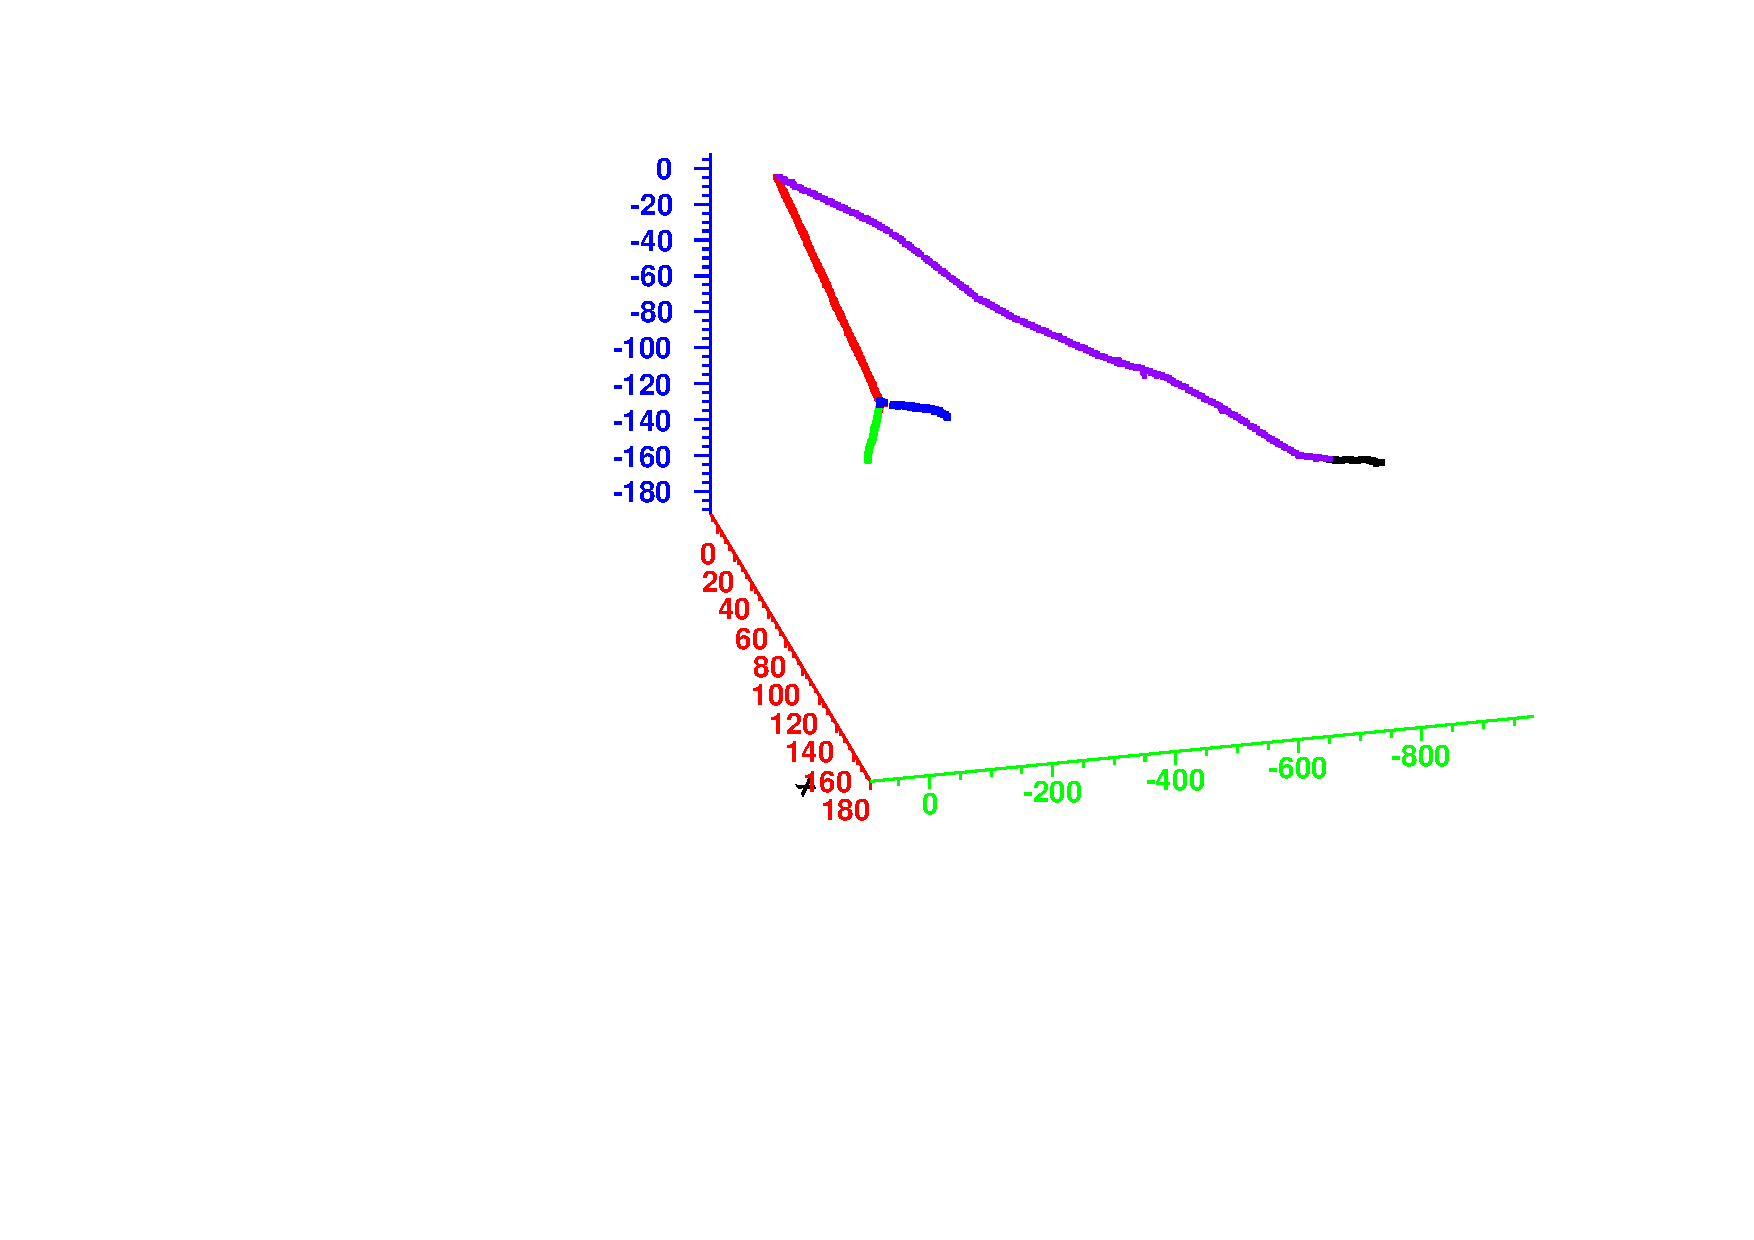
\includegraphics[angle=-90,width=0.6\textwidth]{chapters/cellularautomaton_images/event_366_mu_decay_p_hadronic}
        \label{fig:ca-clusters-ccqe-decay}
    }
    \subfigure[]{
        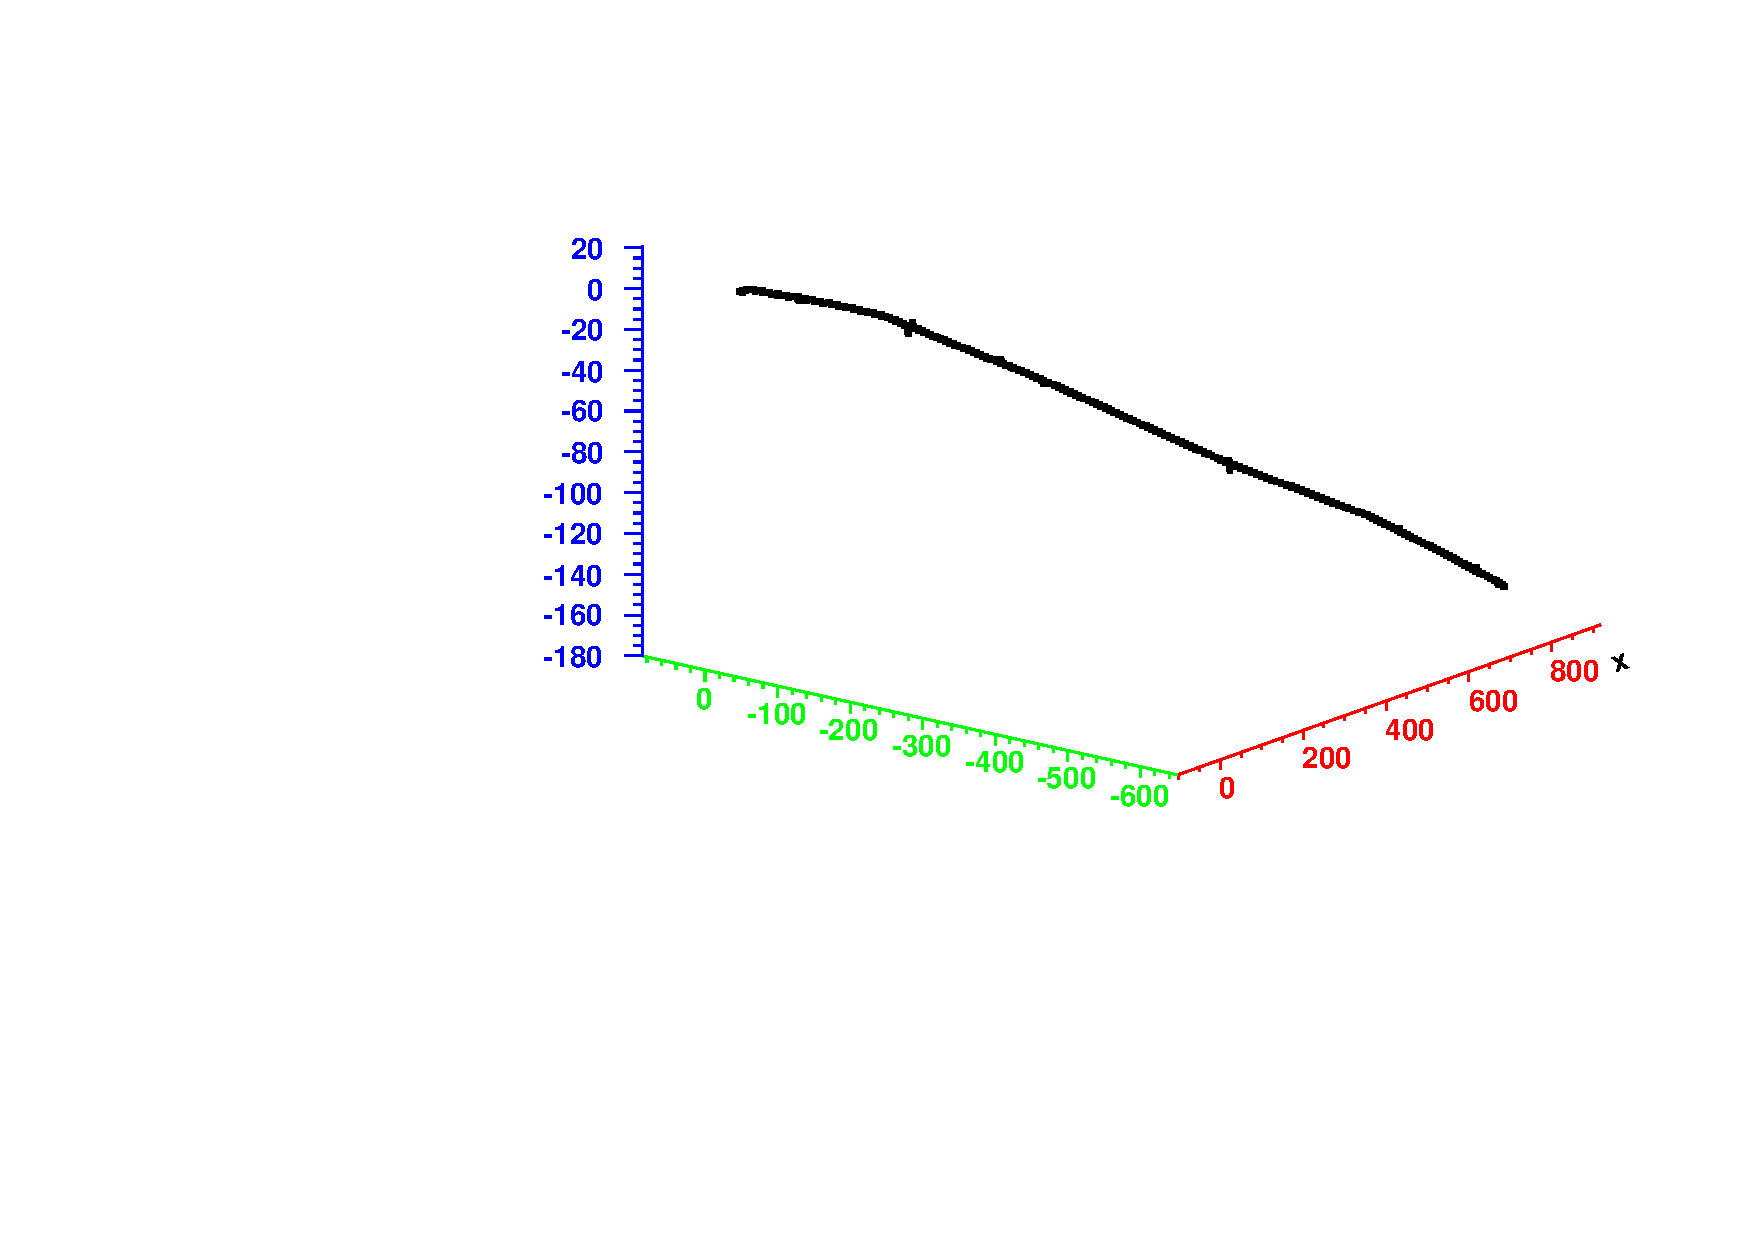
\includegraphics[angle=-90,width=0.6\textwidth]{chapters/cellularautomaton_images/event_986_1tr}
        \label{fig:ca-clusters-ccqe-1tr}
    }
    \caption[Clusters found by the CA in $\ccqe$ events]{\label{fig:ca-clusters-ccqe}Clusters found by the CA in $\nu_\mu$ charged current interactions resulting in $\ccqe$ final states. \subref{fig:ca-clusters-ccqe-2tr} $\mu$ (red) and proton (black) tracks correctly clustered. \subref{fig:ca-clusters-ccqe-decay} $\mu$ track (purple) and Michel electron (black), proton (red) and products of hadronic reinteraction (blue, green). \subref{fig:ca-clusters-ccqe-1tr} an event in which the $\mu$ and proton were produced with nearly identical trajectories and the CA was only able to find one track. Axes are labelled in $\mm$.}
\end{figure}

\begin{figure}
    \centering
    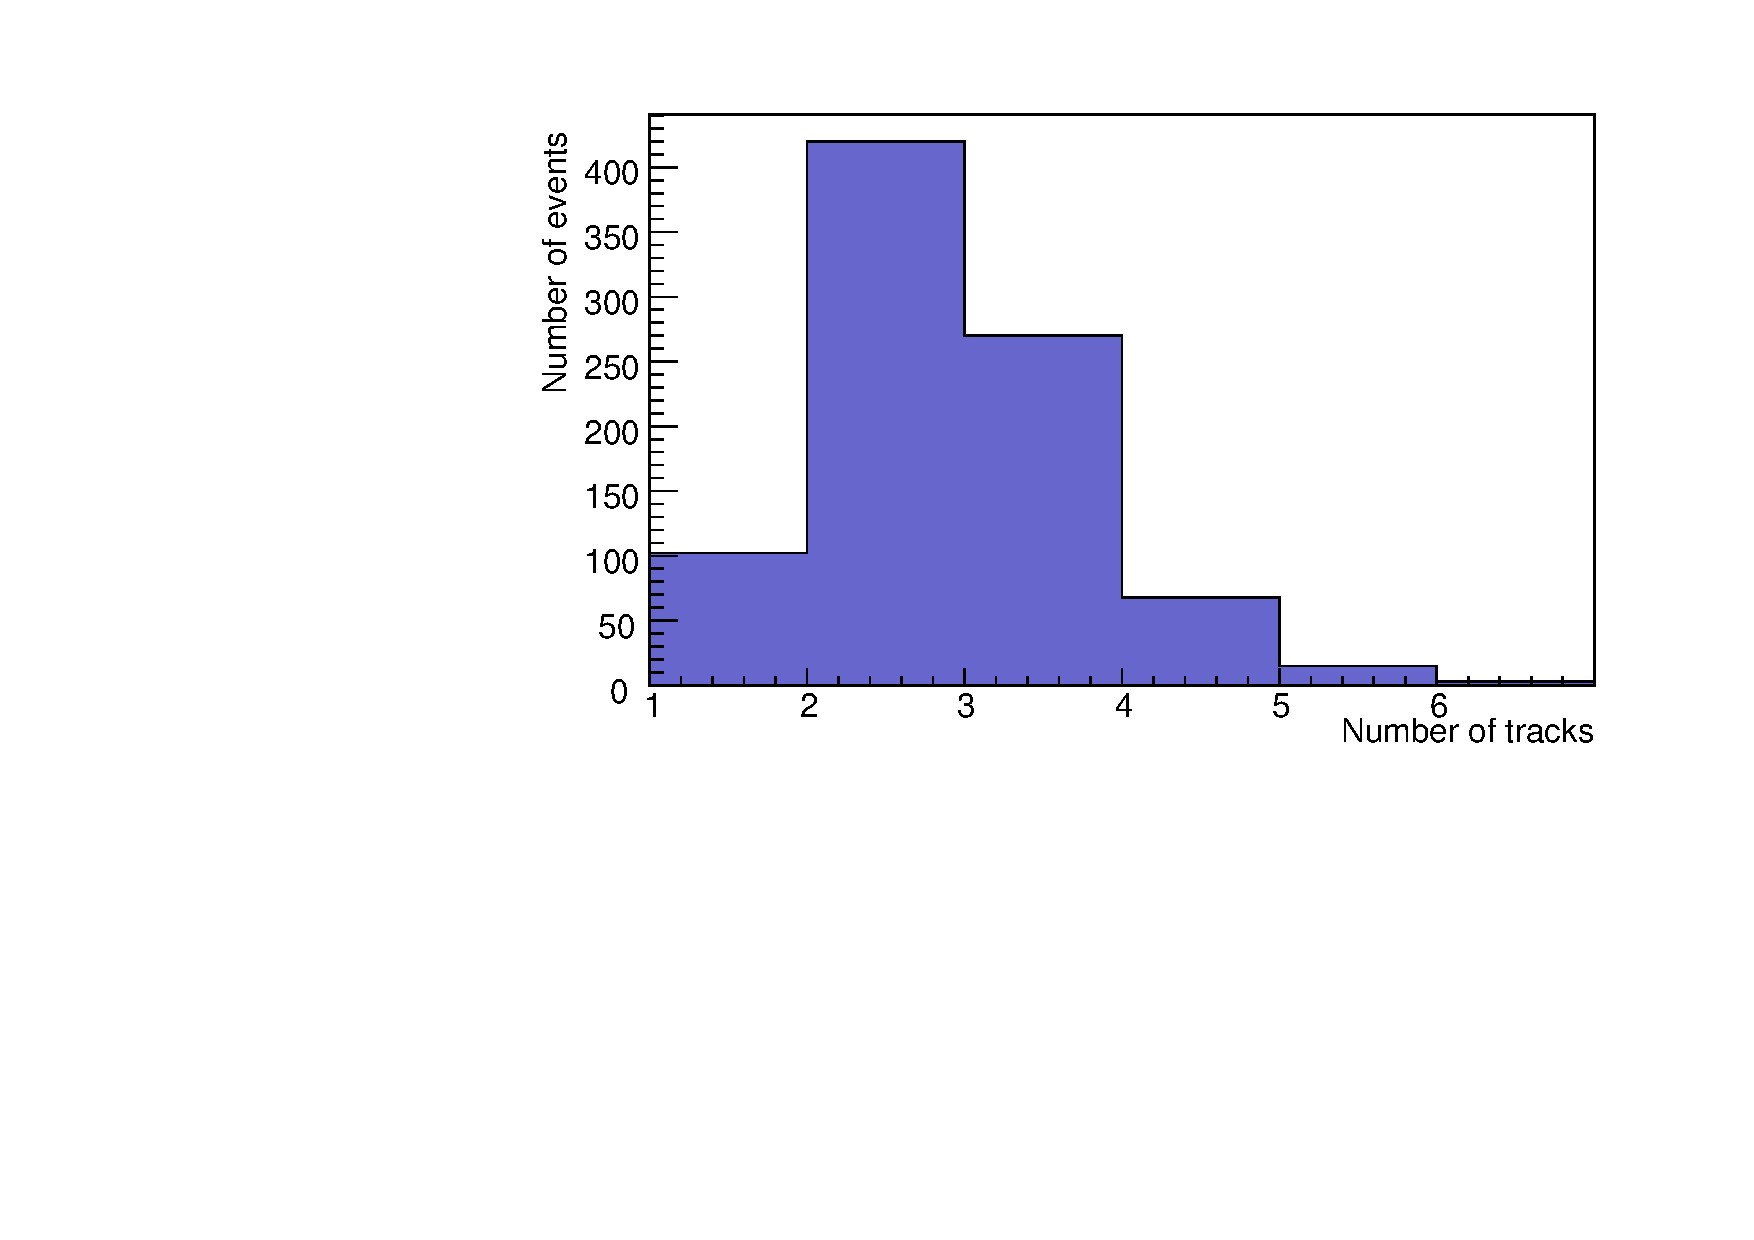
\includegraphics[angle=-90,width=0.8\textwidth]{chapters/cellularautomaton_images/ccqe-trackcount}
    \caption[Number of reconstructed tracks in CCQE events]{\label{fig:ca-ccqe-full-trackcounts}Distribution of reconstructed track counts for CCQE $\nu_\mu$ interactions resulting in $\ccqe$ final states, including hits from secondary particles. Events with a proton track of more than 20 hits were processed, and any trajectory of more than 20 hits was included in the input data. The expectation is to reconstruct two or more tracks (lower numbers are better). 878 events passed the range cut, of which approximately $11\%$ fall into the one-track bin here. The reconstruction can therefore be said to be $89\%$ efficient.}
\end{figure}

\begin{figure}
    \centering
    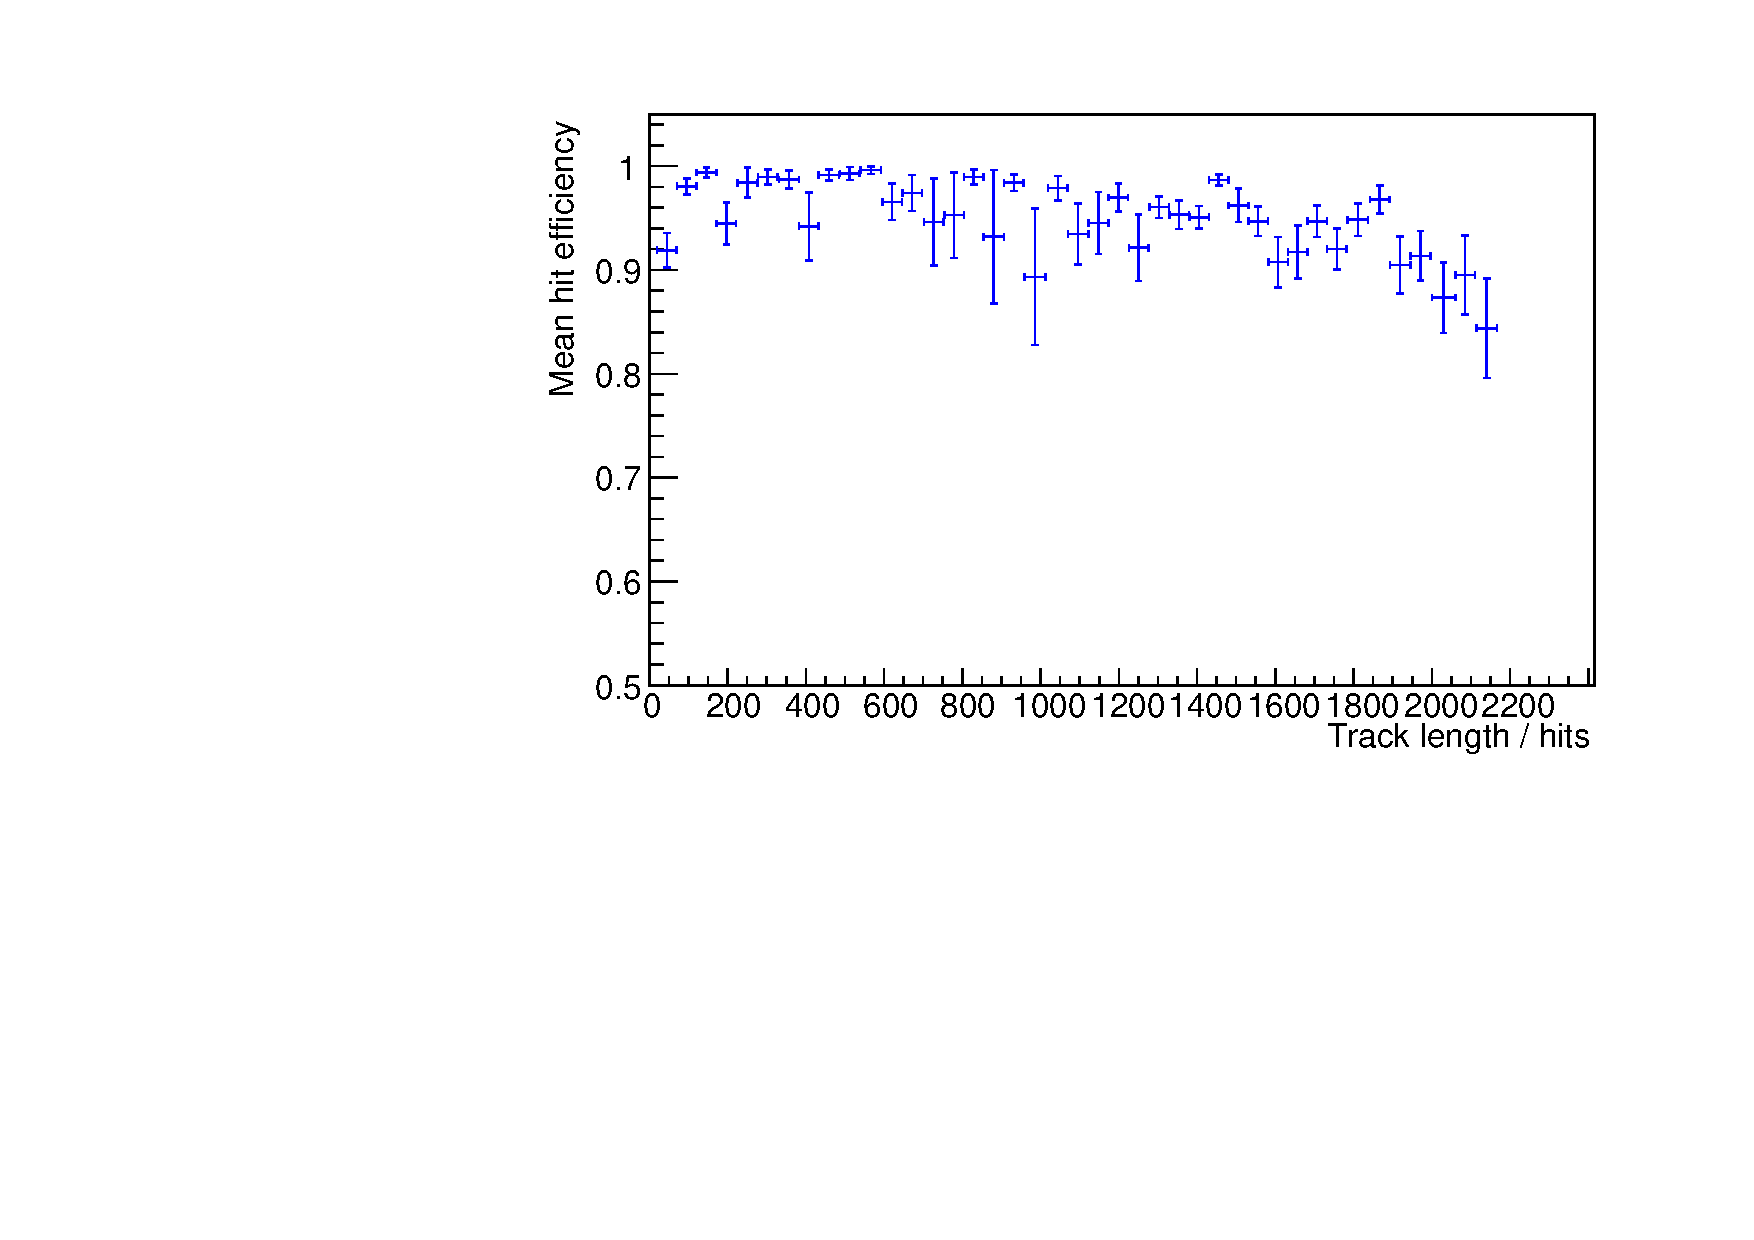
\includegraphics[angle=-90,width=0.8\textwidth]{chapters/cellularautomaton_images/ccqe-efficiency}
    \caption[Hit efficiency for CCQE events reconstructed with a CA]{\label{fig:ca-ccqe-full-efficiency}The hit efficiency (number of hits from the input that remain in an output cluster) for the CA operating on CCQE $\nu_\mu$ interactions with a $\ccqe$ final state. The efficiency is high for all truth track lengths, though the reduction in efficiency towards longer tracks remains.}
\end{figure}

\begin{figure}
    \centering
    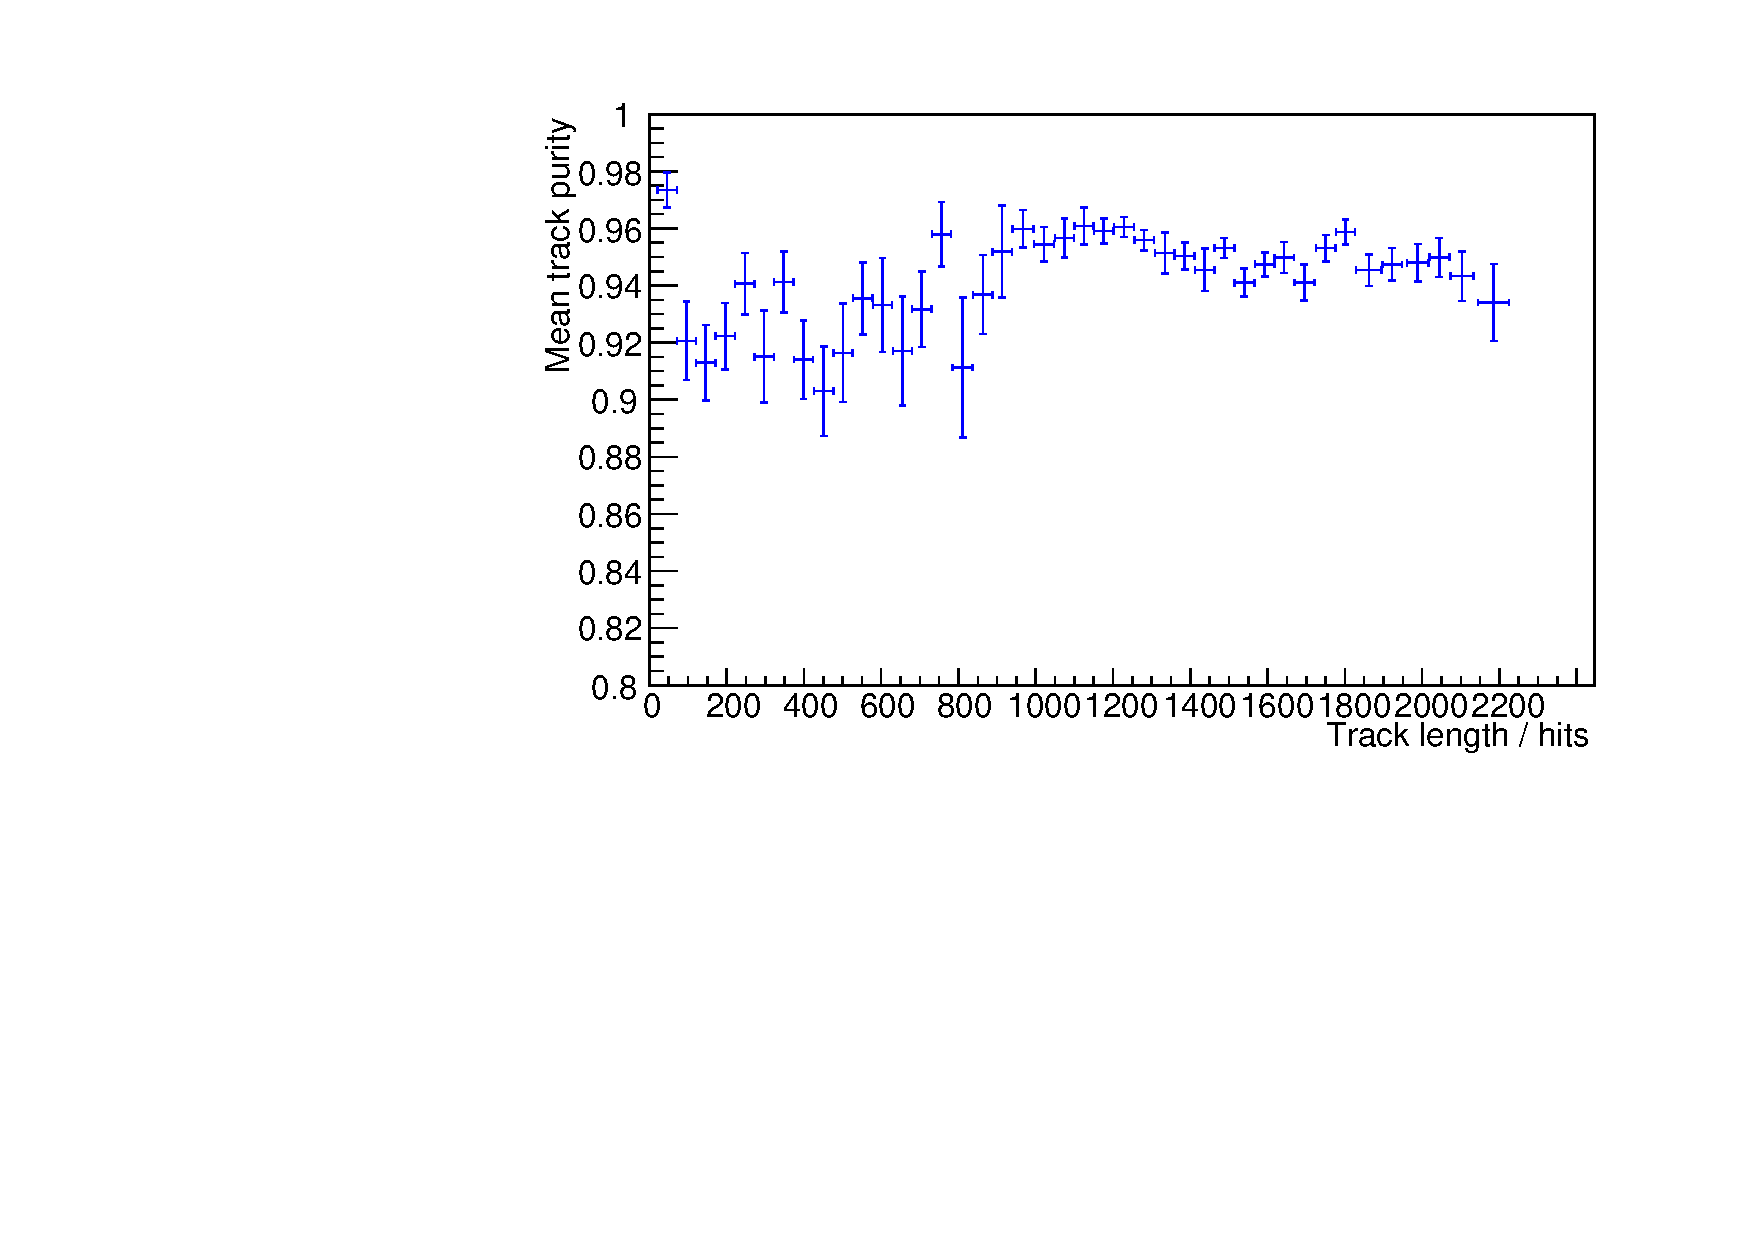
\includegraphics[angle=-90,width=0.8\textwidth]{chapters/cellularautomaton_images/ccqe-purity}
    \caption[Track purity for CCQE events reconstructed with a CA]{\label{fig:ca-ccqe-full-purity}The track purity (fraction of hits within a cluster that originate from the same truth track) for the CA operating on CCQE $\nu_\mu$ interactions with a $\ccqe$ final state. The purity is high for all cluster lengths.}
\end{figure}

Figure \ref{fig:ca-ccqe-full-efficiency} shows the hit efficiency (as defined above) for the full CCQE reconstruction. Here, the drop in efficiency with increasing track length is still present, though the effect is reduced; probably because the additional hits from delta electrons help to smooth out the large scattering angles sometimes present, and allow the \ac{CA} to run through them. Figure \ref{fig:ca-ccqe-full-purity} demonstrates that the \ac{CA} produces extremely pure tracks (over $90\%$ pure) even in situations where hits from delta electrons, decay products and other sources of noise are present. Since one of the main goals of clustering is to obtain collections of related hits, a high purity is very important.

\subsection{Charged Current $\nu_\mu \rightarrow \ccpi$ (CCPi)}
A small fraction of low energy neutrino charged current interactions will produce a charged pion in the final state, mostly through the production and subsequent decay of nucleon resonances. These events were generated with Genie, taking all charged current interactions at the required energy of $0.77\GeV$ and selecting those with a $\ccpi$ (only) final state. The reconstruction algorithm parameters were identical to those applied to the \ac{CCQE} events, above, i.e. $\theta=10\degree$, $R_w=5.0\mm$ and $R_m=30.0\mm$. Once again, 1000 events were generated, and a range cut of 20 hits imposed on both the proton and pion tracks, leaving 891 events for reconstruction.

In principle, the task of reconstruction is more challenging for these events due to the additional final state particle when compared to the CCQE events. In practice, the \ac{CA} handles these events with little degradation of performance. Figure \ref{fig:ca-ccpi-trackcounts} shows the distribution of number of tracks reconstructed. More tracks are found, on average, than in the CCQE events, which is to be expected since we must now consider the additional primary particle, decay products from the $\mu$ or $\pi^+$, and delta electrons or hadronic reinteraction of the proton, as before. Only 26 tracks ($3\%$) were reconstructed with fewer than three tracks. The \ac{CA} therefore successfully clusters $97\%$ of these events. Figure \ref{fig:ca-clusters-ccpi} shows an example of the CA output for a $\ccpi$ event in which both the $\mu$ and $\pi^+$ decay.

\begin{figure}
    \centering
    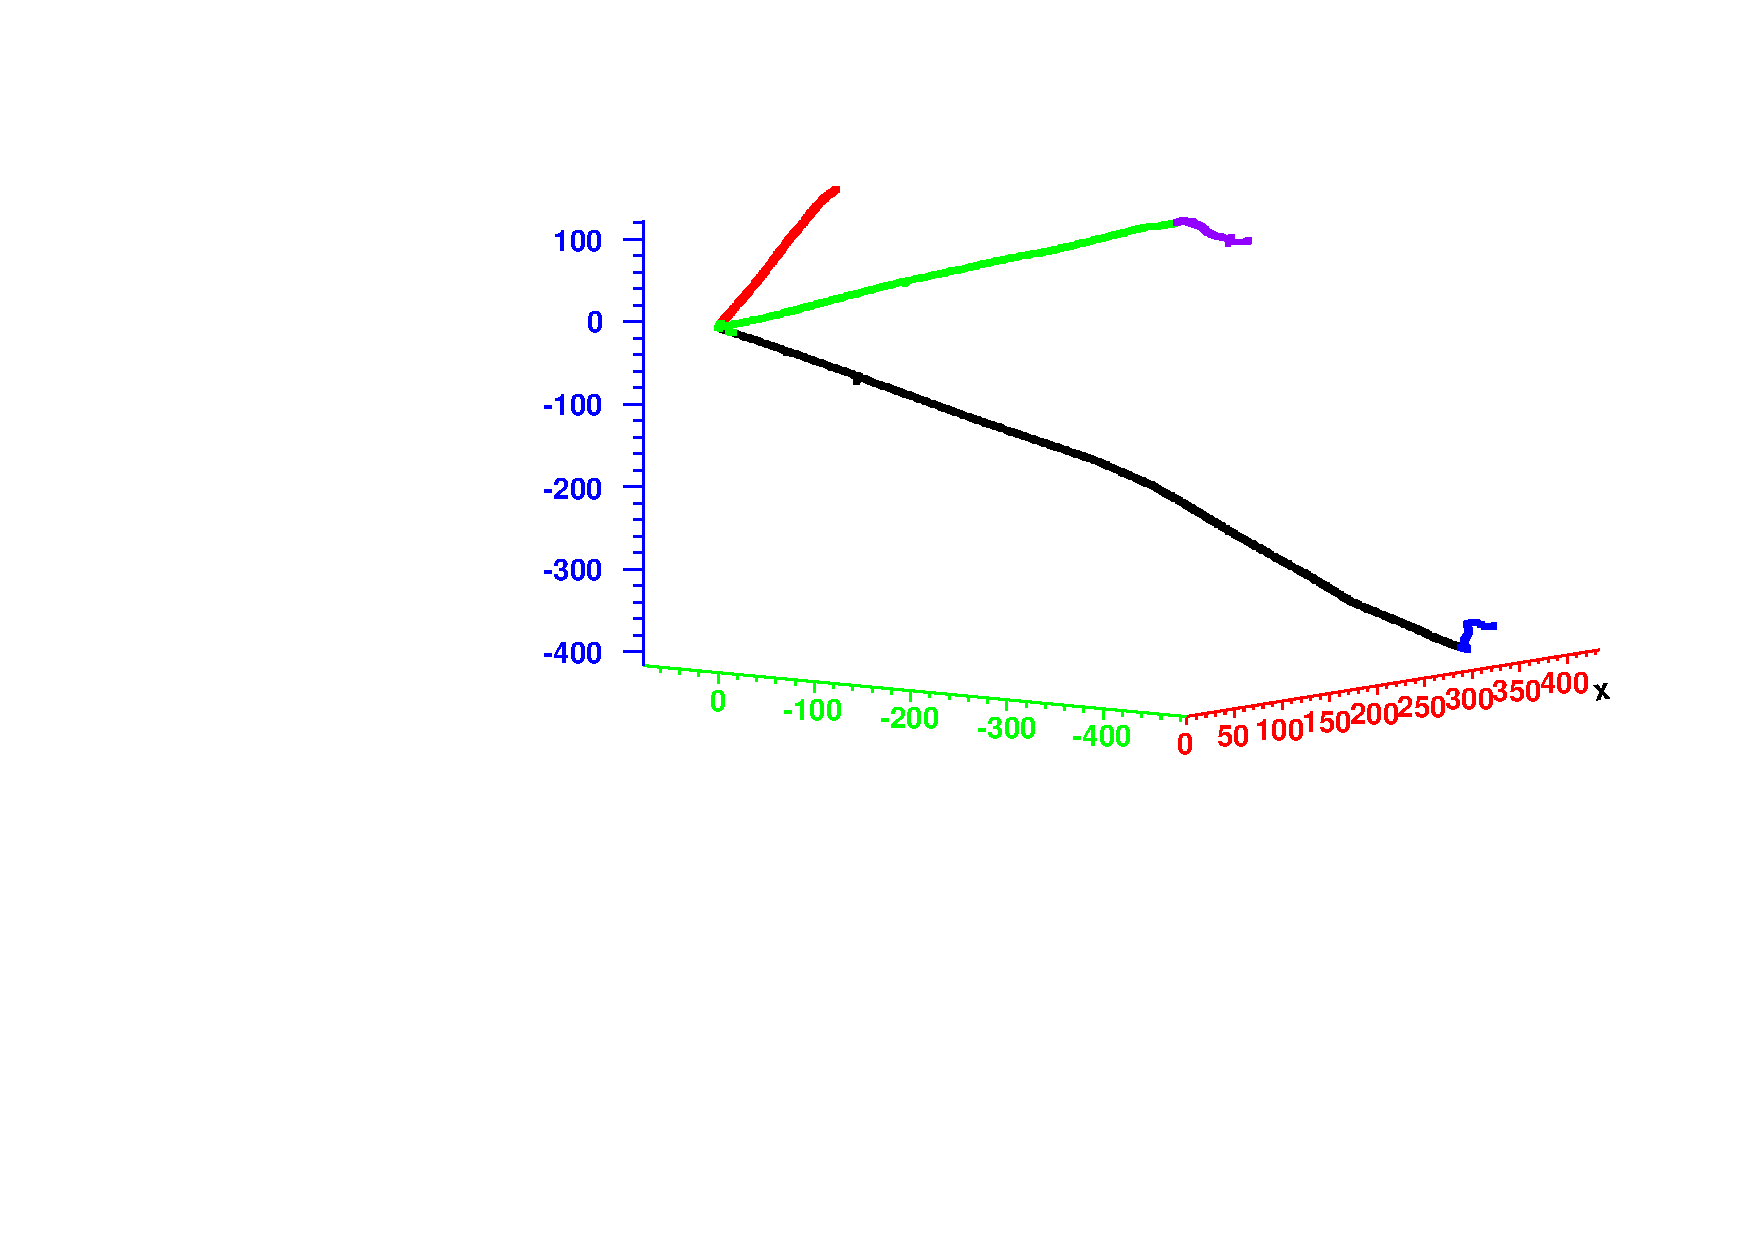
\includegraphics[angle=-90,width=0.7\textwidth]{chapters/cellularautomaton_images/ccpi_bothdecay}
    \caption[Clusters found by the CA in a $\ccpi$ event]{\label{fig:ca-clusters-ccpi}Clusters found by the CA for a charged current $\nu_\mu$ interaction resulting in a $\ccpi$ final state. The $\mu$ and $\pi^+$ both decay within the detector volume, and the CA produces one cluster for each major particle in the event; proton (red), $\pi^+$ (green) and its decay product (purple), the $\mu$ (black) and its Michel electron (blue). Axes are labelled in $\mm$.}
\end{figure}

\begin{figure}
    \centering
    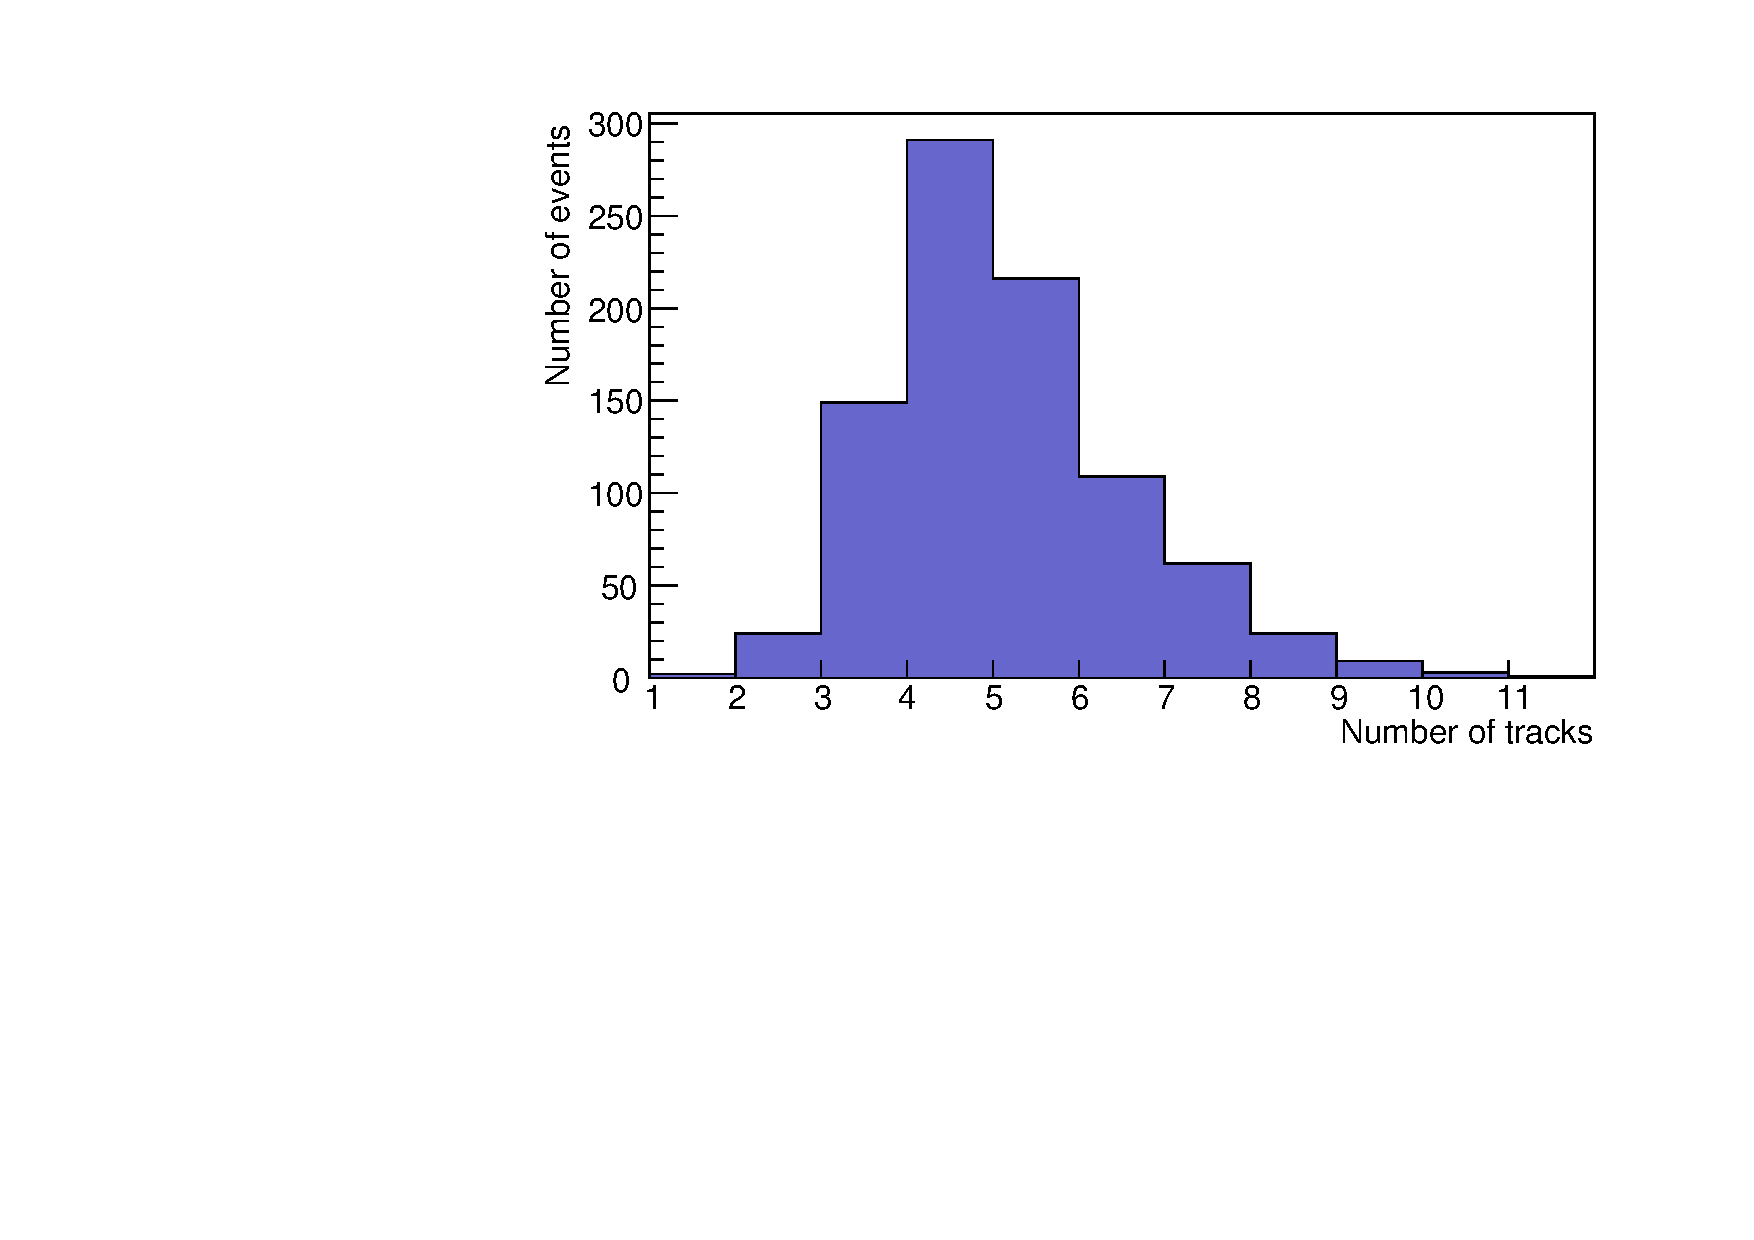
\includegraphics[angle=-90,width=0.8\textwidth]{chapters/cellularautomaton_images/ccpi-trackcounts}
    \caption[Number of reconstructed tracks in CC$\pi$ events]{\label{fig:ca-ccpi-trackcounts}Distribution of reconstructed track counts for charged current $\nu_\mu$ interactions resulting in $\ccpi$ final states, including hits from secondary particles. Events with both proton and pion tracks containing more than 20 hits each were processed, and any trajectory of more than 20 hits was included in the input data. The expectation is to reconstruct at least three tracks, typically more. 891 events passed the range cut, of which approximately $3\%$ were reconstructed with fewer than three tracks.}
\end{figure}

\begin{figure}
    \centering
    \includegraphics[angle=-90,width=0.8\textwidth]{chapters/cellularautomaton_images/ccpi-efficiency}
    \caption[Hit efficiency for CC$\pi$ events reconstructed with a CA]{\label{fig:ca-ccpi-efficiency}The hit efficiency (number of hits from the input that remain in an output cluster) for the CA operating on $\nu_\mu$ charged current interactions with a $\ccpi$ final state. The efficiency is high for all track lengths, but exhibits the same decline with increasing track length as found in the CCQE reconstruction.}
\end{figure}

\begin{figure}
    \centering
    \includegraphics[angle=-90,width=0.8\textwidth]{chapters/cellularautomaton_images/ccpi-purity}
    \caption[Track purity for CC$\pi$ events reconstructed with a CA]{\label{fig:ca-ccpi-purity}The track purity (fraction of hits within a cluster that originate from the same truth track) for the CA operating on $\nu_\mu$ charged current interactions with a $\ccpi$ final state. Short tracks exhibit low purity here, most likely because the addition of a final state $\pi^+$ means that the region around the neutrino interaction vertex is more densely populated than in the CCQE case. High purity is regained for longer tracks, i.e. away from the vertex along the $\mu$ track.}
\end{figure}

The hit efficiency (figure \ref{fig:ca-ccpi-efficiency}) for reconstruction of $\ccpi$ final states is high, but has the same characteristic tail-off with increasing track length. This reinforces the reasoning that the tail-off is due to large scattering events in the muon tracks as the particles deposit energy and slow down. The purity (figure \ref{fig:ca-ccpi-purity}) is lower than the CCQE case for short tracks, but this is expected because the region around the neutrino interaction vertex is more densely populated, making it harder for the CA to correctly cluster the hits. Further out, away from these sources of noise, the CA performs as well as in the CCQE case, and the purities of long tracks in CC$\pi$ events are comparable to those from the CCQE events.

\section{Conclusions}
The \ac{CA} performs three-dimensional clustering with high efficiency, resulting in clusters of high purity (typically over $90\%$). There are a number of parameters that affect the operation of the algorithm, and these must, to an extent, be tuned to the particular application; for example the parameters providing optimal results for clean straight tracks differ from those used to reconstruct noisy physics tracks. The resulting clusters typically require further processing, such as merging and track fitting, but as a tool for hit association, the CA performs well when applied to the typical \ac{LAr TPC} data with high hit densities.

Most of the inefficiencies have topological causes; typically large angular deviations from straight lines, or a high density of tracks close to a vertex, both of which reduce the ability of the CA to produce a small number of pure clusters. Much of this inefficiency could be recovered by applying other algorithms, such as the feature detection algorithm of chapter \ref{sec:latte_feature_detection} to locate interaction and decay vertices, then removing hits in a small sphere around those features. This would leave simpler line-like objects for the CA to work with. Another approach might be to explicitly include the charge deposits as an additional `coordinate', linking together only those cells that form a consistent ionisation energy loss profile.

The CA could be used as part of a larger reconstruction package not only to find and cluster tracks, but also to remove track-like objects prior to shower characterisation and analysis. The identification and analysis of electromagnetic and hadronic showers is an important goal for software reconstruction of events in LAr TPCs, where it is complicated by the homogeneous nature of the detector allowing tracks and showers to develop alongside each other.

In conclusion, the use of a cellular automaton to perform three-dimensional reconstruction of tracks in liquid Argon data is a useful addition to the current knowledge base surrounding \ac{LAr TPC} reconstruction, and is particularly powerful when used as part of an integrated reconstruction package, where its inefficiencies can be compensated with other algorithms.


\chapter{Track Fitting}\label{chapter:KalmanFilter}

\section{Introduction}
Track fitting is the process by which track parameters are determined from a collection of clustered hits. The track parameters include the trajectory, as well as kinematic variables such as the energy or momentum of the particle in question. Track fitting in particle physics is typically performed using a variant of the Kalman filter, which is the optimal estimator for the state of a discrete linear dynamic system.

Originally devised as a noise-reduction and signal filtering technique for communications, the Kalman filter determines optimal estimates of past, present and future states of a linear system based on a series of time-ordered measurements used in conjunction with a statistical model of the system and its measurement errors. It is used extensively for both track and vertex fitting in particle physics, most often in a magnetised detector, where it separates the curvature of a particle due to the magnetic field from the noise introduced by direction changes as a result of multiple scattering.

\section{The Icarus Kalman Filter}
The Icarus~\citep{Amerio2004} experiment presented a Kalman filter~\citep{Fruhwirth1987} which makes statistical use of the distribution of the multiple scattering angle $\theta$ to measure the momentum of a particle in a non-magnetised detector~\citep{Ankowski2006}. The Kalman filter is used to filter out the noise introduced by limited detector resolution. The details of the Icarus algorithm are presented here as an overview of the mechanism of action of the Kalman filter, but also as the basis for the Latte Kalman filter, which aims to perform the same task.

The Kalman filter operates on a discrete set of states, each represented by a state vector $\vec{x}_k$. These states correspond to points on the track, and can in principle be measured anywhere along it. In practice, the track is split into segments of fixed length, and the endpoints of these segments define the set of planes at which the state vector $\vec{x}_k$ is evaluated. 

The track system is described by the linear equation:~\citep{Ankowski2006}
\begin{equation}\label{eqn:kalman_track_system}
    \vec{x}_k^{-} = F_{k-1} \vec{x}_{k-1} + \vec{w}_{k-1}
\end{equation}
Here, $F_{k-1}$ is a matrix defining the propagation of the state vector from plane $k-1$ to plane $k$, $\vec{w}_{k-1}$ is the noise associated with this propagation (which is random, in liquid Argon) and acts to smear the state vector, $\vec{x}_{k-1}$ is the filtered state vector in plane $k-1$, and $\vec{x}_k^{-}$ is the predicted state vector in plane $k$.

The state vector is not usually observed directly; instead, quantities such as the scattering angle are observed, and these are related to quantities in the state vector (such as the particle momentum) through a transformation matrix:
\begin{equation}\label{eqn:kalman_measurement_equation}
    \vec{m}_k = H_k \vec{x}_k + \vec{\epsilon}_k
\end{equation}
where $H_k$ is a matrix transforming a measurement vector $\vec{m}_k$ into a state vector $\vec{x}_k$, and $\vec{\epsilon}_k$ represents measurement noise (errors on the measurements).

The process noise $\vec{w}_k$ and the measurement noise $\vec{\epsilon}_k$ are taken to be unbiased and with finite variance. The covariance matrices are $Q_k$ (for process covariance) and $V_k$ (for measurement covariance). If the process and measurement noise are both random Gaussian variables, the Kalman filter will be the optimal estimator of the system state.

The Kalman filter proceeds through the following three steps, repeated for each new plane $k$ and its corresponding measurement $\vec{m}_k$.

\vspace{1em}\hrule\vspace{1em}
\begin{description}
    \item[1. Prediction:] Given the state vector $\vec{x}_{k-1}$ in plane $k-1$, the prediction step of the Kalman filter estimates the state vector in a future plane $k$, in the absence of noise. The state $\vec{x}_k^{-}$ is the predicted state at plane $k$, using the information contained in all of the state vectors up to $k-1$.
    \begin{equation}\label{eqn:kalman_prediction_step}
        \vec{x}_k^{-} = F_{k-1} \vec{x}_{k-1}
    \end{equation}

    \item[2. Filtering:] Given a predicted state vector $\vec{x}_k^{-}$ (or a suitable initial state), the filtering step determines the present state $\vec{x}_k$ by taking into account the measurements of all previous planes (via the predicted state) and the current plane (via the measurement $\vec{m}_k$). Since the previous measurements are included via their contribution to the state vector, the Kalman filter automatically includes correlations between measurements.
    \begin{equation}\label{eqn:kalman_filtering_step}
        \vec{x}_k = \vec{x}_k^{-} + K_k \left(\vec{m}_k - H_k\vec{x}_k^{-} \right)
    \end{equation}
    where $K_k$ is the Kalman gain matrix, and is related to the covariance of the state vector and the measurement noise.

    \item[3. Smoothing:] When the filter is applied to plane $k+1$, a smoothing step can be used to improve the estimate of the state at plane $k$, taking into account all measurements up to and including $k+1$.
    \begin{equation}
        \vec{x}_k^{n} = \vec{x}_k + A_k \left(\vec{x}_{k+1}^n - \vec{x}_{k+1}^{-}\right)
    \end{equation}
    where $A_k$ is a smoothing gain matrix and $\vec{x}_k^n$ is the filtered state vector after smoothing, for plane $k$.
\end{description}
\vspace{1em}\hrule\vspace{1em}

For particles moving in a non-magnetised detector, the trajectory is split into small track segments, each fitted to a straight line. The state vector $\vec{x}_k$ contains the inverse momentum, coordinates, and track slopes:
\begin{equation}\label{eqn:kalman_state_vector}
    \vec{x}_k = \left( \begin{array}{c} \frac{1}{p} \\ x \\ y \\ \frac{dx}{dz} \\ \frac{dy}{dz} \end{array} \right)
\end{equation}

The transportation matrix $F_k$ provides a straight line extrapolation, with no changes to the track parameters. The energy deposited in a track segment (which can be determined from the charge collected) is subtracted from the momentum estimate in plane $k-1$ to update the momentum estimate in the state vector for plane $k$.

\begin{equation}\label{eqn:kalman_transportation_matrix}
    F_k = \left( \begin{array}{ccccc}
    \frac{1}{1-E_{\mathrm{dep}}/p}  &   0   &   0   &   0       &   0       \\
    0                               &   1   &   0   & \Delta z  &   0       \\
    0                               &   0   &   1   &   0       & \Delta z  \\
    0                               &   0   &   0   &   1       &   0       \\
    0                               &   0   &   0   &   0       &   1
    \end{array} \right)
\end{equation}

The measurement vector includes the coordinates and slopes, but not the inverse momentum. Instead, the angle $\theta_0$ between adjacent track segments at the plane $k$ is used; these angles build up a $\thetarms$ measurement, which is fed to the Kalman filter. Equation \eqref{eqn:kalman_theta_p_relationship} relates this scattering angle to the momentum~\citep{Eidelman2004}.
\begin{equation}\label{eqn:kalman_theta_p_relationship}
    \thetarms = \frac{13.6\MeV}{\beta c p} z \sqrt{\frac{l}{X_0}} \left(1 + 0.038\ln\left[\frac{l}{X_0}\right]\right)
\end{equation}
where $\beta$ is the velocity of the particle, $p$ is its momentum and $z$ is the charge, $X_0$ is the radiation length and $l$ the track segment length. The measurement vector $\vec{m}_k$ is then:
\begin{equation}\label{eqn:kalman_measurement_vector}
    \vec{m}_k = \left( \begin{array}{c} \thetarms \\ x \\ y \\ \frac{dx}{dz} \\ \frac{dy}{dz} \end{array} \right)
\end{equation}

The matrix $H_k$, which relates the measurement and state vectors, is given by:
\begin{equation}\label{eqn:kalman_measurement_matrix}
    H_k = \diag \left( C, 1, 1, 1, 1 \right)
\end{equation}
where $C$ is the constant multiplying $\displaystyle \frac{1}{p}$ in equation \eqref{eqn:kalman_theta_p_relationship}.

Finally, the covariance matrices $Q_k$ (for the system covariance) and $V_k$ (for the measurement covariance) must be taken into account. The Icarus experiment use system covariance matrices from \citep{Wolin1993}, where the covariances for multiple scattering are carefully derived, while the measurements are assumed to be uncorrelated, and the matrix $V$ is diagonal, with each component representing the measurement error.

\section{The Latte Kalman Filter}
The Latte Kalman filter follows closely the formulation used in the Icarus filter. The implementation is based on that present in the SciPy~\citep{SciPy} package for scientific programming in the Python language, with a linear system corresponding to the track fitting mechanism used by Icarus.

The state vector $x_k$ is:
\begin{equation}\label{eqn:kalman_latte_state_vector}
    x_k = \left(\begin{array}{c}
        \frac{1}{p} \\ y \\ z \\ \frac{\Delta y}{\Delta x} \\ \frac{\Delta z}{\Delta x}
    \end{array}\right)
\end{equation}

The measurement vector is identical to the state vector, except for the scattering angle $\thetarms$ in place of the inverse momentum:
\begin{equation}\label{eqn:kalman_latte_measurement_vector}
    x_k = \left(\begin{array}{c}
        \thetarms \\ y \\ z \\ \frac{\Delta y}{\Delta x} \\ \frac{\Delta z}{\Delta x}
    \end{array}\right)
\end{equation}


The process covariance matrix $Q$ is a $5\times 5$ matrix defined as:~\citep{Wolin1993}
\begin{equation}\label{eqn:kalman_process_covariance_matrix}
    Q = \left(
    \begin{array}{ccccc}

        \left(\frac{0.01}{p}\right)^2 &                 0 &                 0 &                0 &                0 \\
                                    0 & \Delta x^2 P_{33} & \Delta x^2 P_{34} & -\Delta x P_{33} & -\Delta x P_{34} \\
                                    0 & \Delta x^2 P_{34} & \Delta x^2 P_{44} & -\Delta x P_{34} & -\Delta x P_{44} \\
                                    0 & -\Delta x P_{33}  & -\Delta x P_{34}  & P_{33}           & P_{34}           \\
                                    0 & -\Delta x P_{34}  & -\Delta x P_{44}  & P_{34}           & P_{44}           

    \end{array}
    \right)
\end{equation}
where $p$ is the momentum at that step, $\Delta x$ is the segment length in the $x$ direction, and
\begin{align*}
    P_{33} &= \theta (1 + S_y^2)(1 + S_y^2 + S_z^2) \\
    P_{34} &= \theta S_y S_z(1 + S_y^2 + S_z^2) \\
    P_{44} &= \theta (1 + S_z^2)(1 + S_y^2 + S_z^2)
\end{align*}
where $\theta$ is the scattering angle, and $\displaystyle S_y=\frac{\Delta y}{\Delta x}$ and $\displaystyle S_z = \frac{\Delta z}{\Delta x}$ are the slopes in $y$ and $z$.

The measurement covariance matrix is diagonal, with components representing the measurement uncertainties on the values of $\theta$, $y$, $z$, $\displaystyle\frac{\Delta y}{\Delta x}$ and $\displaystyle\frac{\Delta z}{\Delta x}$ respectively:
\begin{equation}\label{eqn:kalman_measurement_covariance_matrix}
    V = \diag \left( 1\times10^{-4}, ~ 0.1, ~ 0.1, ~ 1\times10^{-3}, ~ 1\times10^{-3} \right)
\end{equation}

Tracks are split into segments of length $L$ (in $\mm$), with the Kalman filter applied to the points between two segments, and using the slopes of those segments to determine the scattering angle $\theta$ and the distribution of those angles to establish $\thetarms$. The segment lengths are chosen to be a multiple of the radius $R$ (in $\mm$) used for a charge smoothing process which reduces the total number of hits in the track, replacing groups of hits with a single charge-weighted hit. The track momentum is taken from the first component of the state vector after running along the entire track.

\section{Tuning the Kalman Filter}\label{sec:kalman-tuning}
The majority of parameters for the Kalman Filter are fixed by either the process itself (the description of multiple scattering that relates scattering angles to momenta) or by the measurement errors. The remaining free parameters are $R$ and $L$, the charge smoothing radius and segment length, respectively.

A sample of single muon events was generated using the Lamu simulation, producing 100 muons at each energy in the range $100$ to $5000\MeV$ in $100\MeV$ increments. The muon hits from these events were processed using the Kalman filter, and the resulting momentum measurements recorded. The true momentum $p$ is related to the initial kinetic energy $T$ by:\footnote{$E^2 = p^2+m^2$ and $E = T + m$, so $p^2 + m^2 = T^2 + m^2 + 2\,T m$ and the result above can be obtained by a cancellation of $m^2$ followed by the square root operator. This of course assumes natural units, i.e. $c=1$.}
\begin{equation}\label{eqn:momentum-kinetic-energy-relationship}
p = \sqrt{T^2 + 2\,T m}
\end{equation}
where $m$ is the mass of the muon, $105.6583715\MeV$~\citep{PDG2011}.

The segment length was initially chosen to be six times the charge smoothing radius, and the radius varied between $20.1\mm$ and $50.1\mm$. Figure \ref{fig:kalman-mu-momentum-charge-radius-variations} shows the resulting measurements, represented by the mean reconstructed momentum as a function of the true momentum. Smaller smoothing radii ($20.1\mm$) give smaller standard deviation in the results, especially at high momentum, while the mean values are closer to the true momentum for larger smoothing radii of $30.1\mm$ to $40.1\mm$. The distributions of residuals (defined as $p_{\mathrm{true}} - p_{\mathrm{recon}}$) are presented in figure \ref{fig:kalman-residuals} for each of the radii considered here. At momenta over approximately $500\MeV$, the Kalman filter underestimates the momentum when used with short ($20.1\mm$ and $30.1\mm$) segment lengths, but overestimates it for larger segment lengths. As the segment length increases, the range of momentum estimates also increases (both in the positive and negative directions). The Kalman filter in this configuration does not, therefore, provide reliable estimates of momentum.

\begin{figure}
\centering
\includegraphics[angle=-90,width=\textwidth]{chapters/trackfitting_images/kalman-mu-momentum-reconstruction}
\caption[Reconstructed momenta for various Kalman filter parameters]{\label{fig:kalman-mu-momentum-charge-radius-variations}The mean and standard deviation of reconstructed momenta as a function of the true momenta of single muons after application of the Kalman filter, for four values of the charge smoothing radius $R$ (and consequently the segment length $L=6R$).}
\end{figure}

\begin{figure}
\centering

\subfigure[$R=20.1\mm$]{
    \includegraphics[angle=90,width=0.4\textwidth]{chapters/trackfitting_images/r20}
    \label{fig:kalman-residuals-20}
}
\subfigure[$R=30.1\mm$]{
    \includegraphics[angle=90,width=0.4\textwidth]{chapters/trackfitting_images/r30}
    \label{fig:kalman-residuals-30}
}
\subfigure[$R=40.1\mm$]{
    \includegraphics[angle=90,width=0.4\textwidth]{chapters/trackfitting_images/r40}
    \label{fig:kalman-residuals-40}
}
\subfigure[$R=50.1\mm$]{
    \includegraphics[angle=90,width=0.4\textwidth]{chapters/trackfitting_images/r50}
    \label{fig:kalman-residuals-50}
}

\caption[Momentum residuals for various Kalman filter parameters]{\label{fig:kalman-residuals}Residuals (reconstructed momentum minus true momentum) for the Kalman filter with different values of the charge smoothing radius $R$, and therefore of the segment length $L=6R$. The gaps around $1000\MeV$ are due to the $100\MeV$ bin width used. See text for discussion.}
\end{figure}

\section{Momentum Measurements of CCQE \texorpdfstring{$\mu$}{μ} tracks}
In the tuning study of chapter \ref{sec:kalman-tuning}, muons of a fixed kinetic energy (and, therefore, momentum) were used to attempt to validate the Kalman filter algorithm and the choice of parameters. The results indicate that for a $50.1\mm$ charge smoothing radius, and choosing segment lengths six times that radius, the mean momentum measurement is close to the true momentum, but the range of measurements is extremely large.

In this section, the Kalman filter is applied to hits produced by the muon generated from charged current $\nu_\mu$ interactions on Argon nuclei, resulting in $\ccqe$ final states. Two neutrino energies are considered; $E_\nu = 770\MeV$ (1000 events) and $E_\nu = 4.5\GeV$ ($10^4$ events). For the high energy data, the detector simulation was expanded to a cylinder of radius $25\metre$ and height $50\metre$. Muons produced in these interactions have a range of energies and momenta, as well as a distribution of trajectories determined by Genie from the interaction physics models. The true momentum, stored in the Genie event data, was extracted for comparison against the measurements from the Kalman filter. Figure \ref{fig:kalman-ccqe-low} shows the two distributions for the $770\MeV$ neutrinos, and figure \ref{fig:kalman-ccqe-high} shows the distributions for the $4.5\GeV$ neutrinos.

\begin{figure}
\centering
\includegraphics[angle=-90,width=\textwidth]{chapters/trackfitting_images/kalman-ccqe-low}
\caption[True and reconstructed muon momentum distributions at $770\MeV$]{\label{fig:kalman-ccqe-low}Distribution of momenta for muons produced in a charged current low energy $\nu_\mu$ interaction at $770\MeV$ resulting in a $\ccqe$ (only) final state (in red). The distribution of reconstructed momenta (in blue) is from the output of the Kalman filter applied to 1000 such events. The distribution produced by the Kalman filter does not match the true distribution, being both flatter and shifted to higher momentum. The filter therefore overestimates (in general) the momentum of these muons (represented by the shift to higher momentum), but not in a consistent manner (represented by the flatness).}
\end{figure}

\begin{figure}
\centering
\includegraphics[angle=-90,width=\textwidth]{chapters/trackfitting_images/kalman-ccqe-high}
\caption[True and reconstructed muon momentum distributions at $4.5\GeV$]{\label{fig:kalman-ccqe-high}Distribution of momenta for muons produced in a charged current high energy $\nu_\mu$ interaction at $4.5\GeV$ resulting in a $\ccqe$ (only) final state (in red). The distribution of reconstructed momenta (in blue) is from the output of the Kalman filter applied to $10^4$ such events. As for the low energy distribution, the Kalman filter produces overestimates of the muon momentum, though the effect is much more pronounced here.}
\end{figure}

The Kalman filter overestimates the momentum in both the low energy and high energy neutrinos, though the effect is much more pronounced at high energy. Since the method of estimating momentum through the Kalman filter relies on measurements of the multiple scattering angle, these observations correspond to an underestimate of the angle. The angle is more likely to be underestimated at high energy since the effect of scattering is smaller there.

\subsection{Constrained Momentum Measurements}
The data in figure \ref{fig:kalman-mu-momentum-charge-radius-variations} implies that an energy (momentum) dependent choice of the smoothing radius may provide better results, but it is not possible to use this in a general purpose reconstruction algorithm, since the momentum is not known in advance. Indeed, the purpose of applying the Kalman filter is to obtain an estimate of this momentum. The distributions of reconstructed momenta for $E_\nu = 770\MeV$ and $E_\nu = 4.5\GeV$ extend far beyond the energy of the parent neutrino; a situation which is unphysical. Since the maximum possible neutrino energy (i.e. the beam energy) can be known in advance, it is possible to run the Kalman filter in a configuration that enforces constraints on the momentum estimate at each step.

In figure \ref{fig:kalman-constrained-ccqe-770} the distributions of true and reconstructed momenta are shown for $770\MeV$ CCQE interactions resulting in $\mu + p$ final states, where the Kalman filter was constrained such that at each step, the estimated momentum $|\vec{p}|$ must lie between $0\MeV$ and $770\MeV$. The residuals (i.e. the reconstructed momentum minus the true momentum) for this reconstruction are shown in figure \ref{fig:kalman-constrained-ccqe-770-residuals}; the residual is calculated per muon, and a value close to zero indicates compatibility between the true momentum and the reconstructed momentum estimate.

Both plots demonstrate that even with the momentum constrained, the reconstructed values do not agree with the truth. The constraint serves only to truncate all momenta with estimates that would exceed the maximum, resulting in a large peak at the maximum value allowed. From the residuals plot, it is clear that the Kalman filter still over-estimates the momentum of a given track (that is, there are more events on the positive side of the zero point than on the negative side), and that only 5 events out of 1000 have a residual of zero, indicating perfect reconstruction. Many more events have large residuals of over $200\MeV$, and these momentum estimates are not suitable for use in later stages of a general purpose reconstruction chain.

\begin{figure}
    \centering
    \includegraphics[angle=-90,width=\textwidth]{chapters/trackfitting_images/kalman-ccqe-low-constrained}
    \caption[True and reconstructed muon momentum distributions at $770\MeV$ (constrained)]{\label{fig:kalman-constrained-ccqe-770}Distribution of momenta for muons produced in a charged current $\nu_\mu$ interaction at $770\MeV$ resulting in a $\ccqe$ (only) final state (in red). The distribution of reconstructed momenta (in blue) is from the output of the Kalman filter applied to $10^3$ such events, with the momentum estimate at each step constrained such that $0 \le |\vec{p}| \le 770\MeV$. The distributions do not agree, and the highest momentum bin contains almost all of the reconstructed events.}
\end{figure}

\begin{figure}
    \centering
    \includegraphics[angle=-90,width=\textwidth]{chapters/trackfitting_images/kalman-ccqe-low-constrained-residuals}
    \caption[Residuals for constrained momentum reconstruction at $E_\nu = 770\MeV$]{\label{fig:kalman-constrained-ccqe-770-residuals}Residuals (reconstructed momentum minus true momentum) for a Kalman filter performing a constrained momentum reconstruction of muons resulting from $770\MeV$ muon neutrinos interacting in liquid Argon and producing $\ccqe$ (only) final states. Data from $10^3$ events is shown, of which only $5$ have a residual close to zero (which indicates a perfect reconstruction). Most events have a positive residual (which indicates a tendency for the algorithm to over-estimate) and there are many events with large residuals. These results indicate that the algorithm used is not well-suited to this task, and is not capable of delivering accurate momentum estimates on data of this type.}
\end{figure}

The analysis was repeated with $10^4$ muon tracks from interactions of $4.5\GeV$ muon-neutrinos, setting the maximum momentum estimate at each step to $4.5\GeV$. The resulting distribution is shown in figure \ref{fig:kalman-constrained-ccqe-high}, where it is compared to the true distribution. The residuals are not shown, since no events were reconstructed with a momentum less than the maximum allowed by the constraints, hence this reconstruction is no better than simply assuming that each muon carries the maximum possible momentum. These results again demonstrate that the Kalman filter is unfit for the general purpose reconstruction of muon momenta in this environment.

\begin{figure}
    \centering
    \includegraphics[angle=-90,width=\textwidth]{chapters/trackfitting_images/kalman-ccqe-high-constrained}
    \caption[True and reconstructed muon momentum distributions at $4.5\GeV$ (constrained)]{\label{fig:kalman-constrained-ccqe-high}Distribution of momenta for muons produced in a charged current $\nu_\mu$ interaction at $4.5\GeV$ resulting in a $\ccqe$ (only) final state (in red). The distribution of reconstructed momenta (in blue) is from the output of the Kalman filter applied to $10^4$ such events, with the momentum estimate at each step constrained such that $0 \le |\vec{p}| \le 4500\MeV$. The y-axis (number of events) is shown on a log scale. There is no overlap at all between the two distributions; every muon track is reconstructed with the highest allowed momentum.}
\end{figure}

\clearpage
\section{Conclusions}
The Kalman filter is traditionally a powerful tool for track parameter estimation, but in the environment of a \ac{LAr TPC} it does not perform well, at least for the estimation of track momentum. The Icarus experiment achieved better results, but with a smaller measurement error on their individual hits ($400\micron$)~\citep{Ankowski2006}. For data of the type presented here, the Kalman filter (as implemented) is not a good reconstruction tool for the purposes of estimating particle momentum. Attempts to constrain the estimates at each step of the procedure do not improve the end result and serve only as a simple `sanity check' to avoid unphysical reconstructed momenta.

The spatial track parameters were not considered here because muons in liquid Argon undergo frequent large scatters, resulting in tracks that can have substantial curvature or kinks. These track features make it extremely difficult to compare the state of the Kalman filter to the spatial parameters of the whole track, and would have to be considered on a smaller scale, with instantaneous state vectors.


\chapter{Particle Identification}\label{chapter:PID}

\section{Introduction}
Following on from the process of clustering hits together into associated groups, and fitting tracks to obtain parameters such as the slope or particle momentum, it is essential to be able to determine the nature of the particle that produced those hits.

For \ac{CCQE} neutrino interactions it is of critical importance to be able to identify the flavour of the lepton that was produced, and to be able to associate a track with the passage of a muon (if the interaction involved a $\nu_\mu$). Muon identification is often performed with the help of small detector units around the sides of the main detector. A muon typically behaves as a minimum ionising particle, and will often travel all the way through a detector and leave through one of the sides. A signal in such a muon detector is a strong indicator that the track leading into it was produced by a muon.

In the case of a \ac{LAr TPC}, the aim is to fully contain muons (at least, if they are produced somewhere near the centre of the detector volume), and identification must be performed using information from the track reconstruction stage. For the simplest category of charged current interactions, the muon should be represented by the longest track visible in the event, and it is on this basis that the primary identification of muon tracks will be carried out.

For other types of interaction, or for electron neutrinos, there is a much greater chance of an electromagnetic or hadronic shower developing in the event. One advantage often claimed of LAr TPCs is the ability to achieve electron--pion separation by looking at the rate of energy loss, $dE/dx$. Attempts at particle identification based on the properties of electromagnetic or hadronic showers are not considered here, but see \citep{Ramachers2012} for details of one such analysis. Since the homogeneous nature of LAr TPCs allows for the coexistence of tracks and showers, a full analysis framework must be able to cope with showers, in addition to tracks. Furthermore, in order to be applicable to $\nu_e$ events, it must be possible to identify electromagnetic showers and obtain calorimetric information from them, in order to be able to estimate the energy of the incoming $\nu_e$. This is an area in which LAr TPCs should excel, but the focus of this thesis is on track reconstruction techniques; an already difficult area for fully automated reconstruction in such a fine-grained environment.

\section{Muon Track Identification}
In order to be able to select muons based on the track length (approximated as the number of hits contained), it is useful to know the distributions of track lengths for various particle types which may be present in the charged current interactions considered. 

% ************ 0.77 GeV CCQE ************
\subsection{$770\MeV$ $\nu_\mu \rightarrow \ccqe$ (CCQE) Interactions}
This study begins by looking at those distributions for the products of charged current interactions of $770\MeV$ $\nu_\mu$ which produced $\ccqe$ or $\ccpi$ final states, making use of the truth information saved by the simulation. Figure \ref{fig:ccqe-track-lengths-770MeV} shows the distribution of lengths (in terms of number of hits) for muon and proton tracks, and figure \ref{fig:ccqe-electron-lengths-770MeV} shows the distribution of lengths for electron tracks, which are plotted on a different graph because the total number of electron tracks is extremely large, though nearly all such tracks have fewer than 50 hits. These correspond to the delta electrons produced along the length of the other tracks. At neutrino energies around $770\MeV$, there is a strong case to be made for treating all tracks longer than $1000$ hits as muons, resulting in a trade-off between selection efficiency for muons and contamination by protons.

\begin{table}
\centering
\begin{tabular}{*{5}{r}}
 & $\mu$ & $p$ & $e^-$ & $\pi^\pm$ \\
\hline
\hline
Included & 960 & 57 & 0 & 0 \\
Excluded & 40 & 1143 & 67228 & 3 \\
\hline
\end{tabular}
\caption[Composition of tracks after $1000$ hit cut on $770\MeV$ CCQE events]{\label{table:cut-results-ccqe-0.77}Composition of tracks after applying a $1000$ hit cut on the truth tracks from simulation of $770\MeV$ $\nu_\mu$ interactions producing $\ccqe$ final states. The cut selects muon tracks with $96.0\pm0.6\%$ efficiency and $94.4\pm0.8\%$ purity.}
\end{table}

Table \ref{table:cut-results-ccqe-0.77} shows the number of tracks included and excluded by a $1000$ hit cut, where the track type is determined from truth information. Since the electron tracks are produced arbitrarily along the muon track, it is impossible to eliminate electron hits from the muon track, even with clustering techniques such as those provided by the cellular automaton (see chapter \ref{chapter:CellularAutomaton}). The purity of any such tracks will therefore be reduced by the presence of hits from these short delta electron tracks, i.e. reconstructed muon tracks will not be $100\%$ pure at the hit level.


\begin{figure}
\centering
\includegraphics[angle=-90,width=0.8\textwidth]{chapters/particleid_images/particle-lengths-ccqe-770}
\caption[Track length distribution for $\mu$ and $p$ from $770\MeV$ neutrinos (CCQE)]{\label{fig:ccqe-track-lengths-770MeV}Distribution of track lengths, represented as number of hits contained in a track, for muon (blue) and proton (red) tracks produced in charged current interactions of $\nu_\mu$ at $770\MeV$. The distributions are naturally separated at around $1000$ hits.}
\end{figure}

\begin{figure}
\centering
\includegraphics[angle=-90,width=0.8\textwidth]{chapters/particleid_images/electron-lengths-ccqe-770}
\caption[Track length distribution for $e^{-}$ from $770\MeV$ neutrinos (CCQE)]{\label{fig:ccqe-electron-lengths-770MeV}Distribution of track lengths, represented as number of hits contained in a track, for electron tracks produced as secondary particles following charged current interactions of $\nu_\mu$ at $770\MeV$. An extremely large number of very short electron tracks can be seen, corresponding to the production of delta electrons along the length of the trajectories of the primary muon and proton. Most electron tracks have fewer than 50 hits.}
\end{figure}


\clearpage
% ************ 0.77 GeV CCPi ************
\subsection{$770\MeV$ $\nu_\mu \rightarrow \ccpi$ (CCPi) Interactions}
This data set contains 1000 events where a $770\MeV$ $\nu_\mu$ underwent a charged current interaction with an Argon nucleus, producing a $\ccpi$ final state. The distribution of track lengths (represented in terms of the number of hits) for muons, protons and charged pions is shown in figure \ref{fig:ccpi-track-lengths-770MeV}. Here, the separation of muons from other particles by track length alone is not a realistic proposal; although the muons dominate the longer tracks, a number of pion tracks are also long enough to provide significant pollution of the muon selection if track length alone is used to discriminate particle type.

\begin{figure}
\centering
\includegraphics[angle=-90,width=0.8\textwidth]{chapters/particleid_images/ccpi-770-track-lengths}
\caption[Track length distribution for $\mu$, $p$ and $\pi^+$ from $770\MeV$ neutrinos (\acs{CCPi})]{\label{fig:ccpi-track-lengths-770MeV}Distribution of track lengths, represented as number of hits contained in a track, for muon (blue) and proton (red) tracks produced in charged current interactions of $\nu_\mu$ at $770\MeV$ resulting in $\ccpi$ final states. More than $1000$ proton tracks are present, indicating that the $\pi^+$ sometimes produces one or more protons. The distributions are not clearly separated, and while muon tracks are still typically long, there is much more contamination from the other particle species.}
\end{figure}

\clearpage
% ************ 4.5 GeV CCQE ************
\subsection{$4.5\GeV$ $\nu_\mu \rightarrow \ccqe$ (CCQE) Interactions}
This data set contains $10^4$ events in which a $4.5\GeV$ $\nu_\mu$ underwent a charged current interaction with an Argon nucleus, producing a $\ccqe$ final state. The distribution of track lengths (represented in terms of the number of hits) for muons, protons and charged pions (which are produced as secondary particles, in these events) is shown in figure \ref{fig:ccqe-track-lengths-4500MeV}. In addition, a large number of short electron tracks are present, the longest containing only $1238$ hits (in contrast, the muon peak is at 22000 hits).

For these high energy events, it is clear that any track with more than around 5000 hits must correspond to a muon, and the vast majority of muon tracks have between 14000 and 24000 hits. Using the track length to separate muons from other particles should provide an extremely pure selection of muons, in this case. Table \ref{table:cut-results-ccqe-4.5} shows the number of tracks included and excluded by a 5000 hit cut, where the track type is determined from truth information.

\begin{figure}
\centering
\includegraphics[angle=-90,width=0.8\textwidth]{chapters/particleid_images/ccqe-4500-track-lengths}
\caption[Track length distributions for $\mu$, $p$ and $\pi^+$ from $4.5\GeV$ neutrinos (CCQE)]{\label{fig:ccqe-track-lengths-4500MeV}Distribution of track lengths, represented as number of hits contained in a track, for muon (blue), proton (red) and charged pion (orange) tracks produced in charged current interactions of $\nu_\mu$ at $4.5\GeV$ resulting in $\ccqe$ final states. The proton distribution peaks at over $1.55\times10^4$ tracks on the left.}
\end{figure}

\begin{table}
\centering
\begin{tabular}{*{5}{r}}
 & $\mu$ & $p$ & $e^-$ & $\pi^\pm$ \\
\hline
\hline
Included & 9982 & 14 & 0 & 0 \\
Excluded & 32 & 29640 & 11961433 & 1646 \\
\hline
\end{tabular}
\caption[Composition of tracks after $5000$ hit cut on $4.5\GeV$ CCQE events]{\label{table:cut-results-ccqe-4.5}Composition of tracks after applying a $5000$ hit cut on the truth tracks from simulation of $4.5\GeV$ $\nu_\mu$ interactions producing $\ccqe$ final states. The cut selects muon tracks with $99.7\pm0.1\%$ efficiency and $99.9\pm0.1\%$ purity.}
\end{table}

% ************ 4.5 GeV CCPi ************
\subsection{$4.5\GeV$ $\nu_\mu \rightarrow \ccpi$ (CCPi) Interactions}
This data set contains $10^4$ events in which a $4.5\GeV$ $\nu_\mu$ underwent a charged current interaction with an Argon nucleus, producing a $\ccpi$ final state. The distribution of track lengths (represented in terms of the number of hits) for muons, protons and charged pions is shown in figure \ref{fig:ccpi-track-lengths-4500MeV}. The $\pi^+$ and $p$ peaks on the left extend up to $4.3\times10^4$ tracks. In this case, the muons are once again clearly separated, as for the CCQE events at $4.5\GeV$, and a cut at 5000 hits would select almost entirely muon tracks, rejecting those from protons and pions. Table \ref{table:cut-results-ccpi-4.5} shows the number of included and excluded tracks following a 5000 hit cut.

\begin{figure}
\centering
\includegraphics[angle=-90,width=0.8\textwidth]{chapters/particleid_images/tracks-ccpi-4500MeV}
\caption[Track length distribution for $\mu$, $p$ and $\pi^+$ from $4.5\GeV$ neutrinos (CCPi)]{\label{fig:ccpi-track-lengths-4500MeV}Distribution of track lengths, represented as number of hits contained in a track, for muon (blue), proton (red) and charged pion (orange) tracks produced in charged current interactions of $\nu_\mu$ at $4.5\GeV$, resulting in $\ccpi$ final states. The proton and pion peaks on the left extend up to $4.3\times10^4$, and the plot range has been reduced to better display the separation between hadron ($p$ and $\pi$) and lepton ($\mu$) tracks. A cut at 5000 hits would cleanly select muons with low contamination from other tracks.}
\end{figure}

\begin{table}
\centering
\begin{tabular}{*{6}{r}}
 & $\mu$ & $p$ & $e^-$ & $\pi^\pm$ & Other \\
\hline
\hline
Included & 9717 & 24 & 0 & 12 & 12 \\
Excluded & 337 & 67286 & 12854577 & 18691 & 188995 \\
\hline
\end{tabular}
\caption[Composition of tracks after $5000$ hit cut on $4.5\GeV$ CCPi events]{\label{table:cut-results-ccpi-4.5}Composition of tracks after applying a $5000$ hit cut on the truth tracks from simulation of $4.5\GeV$ $\nu_\mu$ interactions producing $\ccpi$ final states. The cut selects muon tracks with $96.6\pm0.2\%$ efficiency and $99.5\pm0.1\%$ purity.}
\end{table}

\clearpage
\subsection{Conclusions}
It is clear from the track distributions presented above that for the low energy $\mu + p$ events, and for the high energy $\ccqe$ and $\ccpi$ events, a simple cut on the minimum track length is sufficient to select muon tracks from an event. The low energy $\ccpi$ events are an exception to this, and present a more complicated case for analysis, which may require further variables to be considered in order to extract muons with high purity. More traditional particle identification mechanisms, which make use of many variables and attempt to categorise events based on likelihood fits or the results of a neural network are not considered here, but may prove useful in cases such as the low energy $\ccpi$, where the interactions of the particles differ considerably, but are not well represented in the track length alone.

For the remaining three event classes (high and low energy CCQE, high energy CCPi) this range cut should retain high efficiency, though it is worth noting that the studies in this chapter consider truth information, and that the effects of a reconstruction algorithm such as the cellular automaton of chapter \ref{chapter:CellularAutomaton} will necessarily reduce the efficiency of such a technique. The cut values are summarised in table \ref{table:summary_cuts}.

\begin{table}
\centering
\begin{tabular}{cccc}
Class & Cut Value (Hits) & Efficiency & Purity \\
\hline
\hline
CCQE $770\MeV$ & 1000 & $96.0\pm0.6$ & $94.4\pm0.8$ \\
CCQE $4.5\GeV$ & 5000 & $99.7\pm0.1$ & $99.9\pm0.1$ \\
CCPi $4.5\GeV$ & 5000 & $96.6\pm0.2$ & $99.5\pm0.1$ \\
\hline
\end{tabular}
\caption[Summary of cuts with efficiencies and purities]{\label{table:summary_cuts}Summary of the cuts for muon selection in different event classes, including the efficiency for selecting muons, and the resulting purity.}
\end{table}


\chapter{Analysis of Neutrino Interactions}\label{chapter:Analysis}
\section{Introduction}
The goal of this thesis is to demonstrate a fully automated reconstruction chain for event data from \ac{LAr TPC}s. Since the details of charge readout and position reconstruction will vary depending on the detector technology and geometry, as well as the equipment used, this study begins from the point at which three-dimensional hit data exists in a persistent on-disk format. This chapter uses the algorithms and techniques presented earlier to attempt to reconstruct physics information such as the muon energy from charged current $\nu_\mu$ interactions at beam energies of $770\MeV$ and $4.5\GeV$.

\section{Charged Current $\nu_\mu \rightarrow \mu + p$ at $770\MeV$}
\subsection{Event Selection Efficiency}
A sample of $1000$ events produced from charged current interactions of $\nu_\mu$ at $770\MeV$, yielding $\mu + p$ (only) final states were considered. These are the same events used for validation of algorithms earlier in this thesis. Of these 1000 events, 878 survive the initial requirement that the true proton track has more than 20 hits and undergo reconstruction. 

Events surviving the initial cut undergo the following reconstruction steps:
\begin{enumerate}
    \item Apply charge weighting using a weighting radius $R_w=5\mm$.
    \item Apply the cellular automaton, using a maximum scattering angle of $30\degree$.
    \item Apply the cylinder-based merging algorithm, using a merging radius $R_m=30\mm$ and allowing infinitely long cylinders.
    \item Select events with two reconstructed clusters after merging.
    \item Select events in which one cluster has $> 1000$ hits, and the other has $< 1000$ hits.
    \item Associate the longer of the two clusters with the muon track.
    \item Associate the shorter of the two clusters with the proton track.
\end{enumerate}

A total of 420 events have only two tracks in the output after merging (events with more tracks in the output can potentially be recovered with improved merging algorithms, or by discarding delta electron tracks). Of these, 407 events have at least one output track containing over 1000 hits (of which, 10 events have both tracks with over 1000 hits). In 341 events, there is one track with over 1000 hits, and one smaller track. The long track is identified from the truth information as corresponding to the muon, and the shorter track is identified from the truth information as corresponding to the proton.

Based on the numbers above, an analysis that required precisely two tracks, one of which had over 1000 hits, and the other with fewer than 1000 hits will recover 397 events from the sample of 1000, of which 341 will be correctly identified as $\mu + p$ events, with the tracks tagged with the right particle type. This corresponds to an efficiency of $397/1000 = 39.7\%$ for selecting $\mu + p$ events, with a purity of $341/397 = 85.9\%$.

While the efficiency of this selection is low (under $40\%$), the purity attained is high (over $85\%$), and as already mentioned it is possible to recover many more events with improvements to the reconstruction chain.

\subsection{Muon Energy Reconstruction}
\subsubsection{Using Number of Hits}
In an ideal scenario, the number of hits in a cluster should correspond approximately to the length of the cluster in $\mm$. Since the range of a muon track varies with the initial energy of the muon, assuming minimum-ionising behaviour throughout, it should be possible to obtain a calibration for conversion between number of hits (or muon track length) and initial muon energy. In practice, the number of hits in an output cluster is a poor estimator for the initial muon energy, as demonstrated in figure \ref{fig:ccqe-770-e-nhits-calib}. One possible reason for this is the loss of hits in the cellular automaton state of the reconstruction; the proportion of lost hits rises with track length, resulting in increasingly poor estimates. However, since the hit loss should occur throughout the track, it may be possible to use the length itself to estimate the energy.

\begin{figure}
    \centering
    \includegraphics[angle=-90,width=0.8\textwidth]{chapters/analysis_images/ccqe-770-e-nhits-calib}
    \caption[Relationship between number of hits and energy]{\label{fig:ccqe-770-e-nhits-calib}The relationship between the number of hits $N$ in a muon cluster and the initial energy $E_\mu$ of the particle, in $\MeV$. The broad distribution indicates that the number of hits is not a good estimator for the energy of the particle, and that calibrations based on this quantity cannot provide reliable energy estimates.}
\end{figure}

\subsubsection{Using Track Length}
Calculating the length of the track is not as simple as taking the ``smallest'' and ``largest'' hits and determining the distance between them, since it is possible that the muon track may undergo significant scattering along its length, and can develop an appreciable curve. In order to determine the track length, an algorithm must run along the track in small steps, adding up the segment lengths as it goes. Such a mechanism can be easily implemented using the \ac{KDTree} structure described in chapter \ref{sec:latte_kdtree}, but this introduces another parameter; the radius used for the neighbour search, which becomes the maximum segment length.

\begin{figure}
    \centering
    \subfigure[$20\mm$]{
        \includegraphics[angle=-90,width=0.45\textwidth]{chapters/analysis_images/seg-20}
    }
    \subfigure[$50\mm$]{
        \includegraphics[angle=-90,width=0.45\textwidth]{chapters/analysis_images/seg-50}
    }
    \subfigure[$100\mm$]{
        \includegraphics[angle=-90,width=0.45\textwidth]{chapters/analysis_images/seg-100}
    }
    \subfigure[$150\mm$]{
        \includegraphics[angle=-90,width=0.45\textwidth]{chapters/analysis_images/seg-150}
    }
    \subfigure[$200\mm$]{
        \includegraphics[angle=-90,width=0.45\textwidth]{chapters/analysis_images/seg-200}
    }
    \subfigure[$300\mm$]{
        \includegraphics[angle=-90,width=0.45\textwidth]{chapters/analysis_images/seg-300}
    }
    \subfigure[$400\mm$]{
        \includegraphics[angle=-90,width=0.45\textwidth]{chapters/analysis_images/seg-400}
    }
    \caption[Relationship between track length and muon energy]{\label{fig:energy-recon-track-length}Relationship between the measured length of a reconstructed track and the true energy of the corresponding muon, shown for segment lengths of $20\mm$, 50\mm$, 100\mm$, 150\mm$, 200\mm$, $300\mm$ and $400\mm$. See text for discussion.}    
\end{figure}

The track length is calculated by taking the clustered set of hits, looking for an \emph{extreme} hit, i.e. one end of the track, then searching for neighbours within some radius $R$. The furthest neighbour becomes the next seed point, and the distance between the two is added to an accumulator variable. This process is repeated, using principal components analysis to ensure that the discovered point is always moving away from the previous steps, until the other end of the track is reached. The sum of step lengths approximates the length of the entire track. The maximum segment length is determined by the value of $R$, and the results of applying this procedure to the $397$ tracks being analysed here are shown in figure \ref{fig:energy-recon-track-length} for seven different maximum segment lengths.

Smaller segment lengths allow for a more accurate estimate of the track length in the presence of curvature, but are more susceptible to gaps in the reconstructed track causing early termination of the algorithm. This can be seen in the results for a $20\mm$ segment length, where most measurements have very small lengths. Longer segment lengths are more tolerant of gaps, but provide poor estimates when traversing curved tracks, as well as reducing the sensitivity to features on a scale smaller than the segment length. This can be seen across the set of graphs, with the cluster of points shifting rightward (i.e. towards longer estimates) with increasing segment length. The results in figure \ref{fig:energy-recon-track-length} indicate that, once again, the correlation between reconstructed track length and true muon energy is poor, and cannot be used to calibrate for energy reconstruction.

\section{Conclusions}
The analysis in this chapter presents one possible approach to the reconstruction of neutrino events in \ac{LAr TPC} environments, using many of the tools and algorithms developed, described and characterised in the rest of this thesis. Although the final step of reconstructing the muon energy was not possible using the techniques applied above, there remain other options for reconstructing physics information, and some of the same procedures could be applied to obtain clusters and produce event selections with a very high purity (over $85\%$). The efficiency of such a selection is low, in part due to the very specific requirements that were imposed, i.e. precisely two reconstructed tracks, one with greater than $1000$ hits, and one with fewer than $1000$ hits. As has already been mentioned, the selection efficiency (under $40\%$) can be boosted by considering additional event classes, for instance the three-track events, with extra merging or further processing.

The techniques presented clearly provide building blocks for the clustering and selection of arbitrary track-like objects, and depending on the physics case, an analysis such as the one described in this chapter could be built from these algorithms, tailored to the specific requirements for identifying the kind of particles of interest. While the analysis presented focused on muons, and was ultimately unable to reconstruct the energy from the two techniques applied, the successful demonstration of clustering and selection of these events stands alone; such automated processing has not been fully demonstrated prior to the work of this thesis.


\chapter{Conclusion}\label{chapter:Conclusion}
A number of algorithms and reconstruction techniques have been introduced in this thesis, and it is worth taking some time to summarize the important results of the characterisation of each.

Chapter \ref{chapter:Latte} introduced a number of algorithms that can be used as building blocks for more complicated reconstruction procedures. In particular, the KDTree has been used to provide near-neighbour search in the cellular automaton of chapter \ref{chapter:CellularAutomaton} and in the length estimation algorithms of chapter \ref{chapter:Analysis}. The KDTree is not a reconstruction algorithm in itself, but is demonstrably useful in the implementation of such algorithms.

Of particular note in chapter \ref{chapter:Latte} is the three-dimensional feature detection, which was demonstrated to correctly identify the primary interaction vertex (as well as a number of other features such as the production sites of delta electrons, and track endpoints) in over $70\%$ of charged current $\nu_\mu$ interactions producing $\ccqe$ final states. The ability to identify these interest points with high efficiency and in three dimensions is a significant result. The technique could be further improved by extending the mathematical operations of the feature detection algorithm to three dimensions, rather than using projections as described in this thesis. Such an extension would take full advantage of the three-dimensional data and may result in more accurate determination of features of interest. However, this task relies on finding a suitable function to produce a scalar \emph{response value} from the response matrix.

The cylinder merging algorithm presented merges hits that fall inside an infinitely long cylinder around a seed track. This is a successful strategy for very sparse events, but with higher track multiplicities, it is possible to have intersecting cylinders from key tracks. In such a situation, stealing hits from one track is not desirable, so the algorithm could be trivially extended by considering only the regions near the end of a track. In events with a high track multiplicity, or with high curvature, such a merging strategy would produce better results than the infinite cylinder method used here.

In order to automate the application of these algorithms to perform reconstruction tasks, the \emph{Latte Control} framework was developed and described in chapter \ref{sec:LatteControl}. This allowed for the prototyping of reconstruction sequences, as well as automating reconstruction in a controllable and customisable way. This framework makes automated reconstruction of \ac{LAr TPC} events possible by simply chaining together correctly configured components, which can perform any task from the initial reconstruction steps through to complex statistical analyses.

Chapter \ref{chapter:CellularAutomaton} introduced a clustering technique based on a cellular automaton. The performance of this algorithm was characterised by applying it to simple two-track straight line events before running on long two-track events from charged current $\nu_\mu$ interctions. The final step was to apply the algorithm to the full set of hits from charged current $\nu_\mu$ interactions producing either $\ccqe$ or $\ccpi$ final states. The resulting clusters were typically of very high purity (over $90\%$) and although some hit loss reduced the hit-level efficiency, many of these hits could be recovered by returning to the raw data and applying a merging algorithm to fill in any dropped hits.

The cellular automaton itself produces small clusters of high purity based on its ability to discriminate between sets of related hits according to how track-like they are, and according to the directionality of those tracks. When applied to straight line two-track events with a large opening angle (i.e. over $140\degree$) this ability to discriminate is diminished; applying feature detection to isolate the vertex and mask out hits in that region may help to improve the clustering in these cases.

Chapter \ref{chapter:KalmanFilter} describes a Kalman filter for muon momentum reconstruction, as presented by the Icarus collaboration. An attempt to re-implement this filter and apply it to muon data from the \emph{Lamu} simulation proved unsuccessful, with no reliable momentum measurements available. It is possible that with further tuning, the Kalman filter may be able to provide realistic momentum estimates from measurements that take into account the multiple scattering of particles in a dense medium, but this will always be an easier task to perform in the presence of a magnetic field, where a helical fit can be applied. Given the large size of planned liquid Argon detectors, a strong magnetic field would be prohibitively expensive, but weaker, non-uniform fields may be sufficient to perform this task. A magnetic field would also provide much needed charge discrimination, e.g. between $\mu^+$ and $\mu^-$.

The cuts applied in chapter \ref{chapter:PID} are for the selection of muons, and apply only to data from the \emph{Lamu} simulation, although the arguments used remain valid for any data source. They were presented primarily to allow for the continuation of an analysis based on selecting events by their clustered properties.

Finally, chapter \ref{chapter:Analysis} describes an attempt to reconstruct the energy of the muon in charged current $\nu_\mu$ interactions at $0.77\GeV$, resulting in $\ccqe$ final states. Events were selected based on being reconstructed with precisely two tracks (after merging), and further refined by requiring that one track had over $1000$ hits, and the other fewer than $1000$ hits, as per the cuts described in chapter \ref{chapter:PID}. This resulted in a selection where each event contains one proton track and one muon track, with efficiency $39.7\%$ and purity $85.9\%$. As stated in the chapter itself, the efficiency is low due to the stringent requirements applied, and could be boosted by applying further merging to events with three or four tracks, based e.g. on eliminating tracks consistent with delta electrons or decay products, and by requiring that tracks considered to be protons and muons originate from the same vertex. In these cases, the information required to perform such an analysis is provided by the algorithms already presented, but there was insufficient time to extend this work to include higher track multiplicities.

A determination of the energy of the muon in each event could not be completed in this thesis, but by improving the merging algorithm to reduce hit loss, and considering the charge deposited (along with the $dE/dx$ profile for a muon in liquid Argon) it should be possible to obtain energy measurements. Indeed, for a fully contained muon track, this should be a matter of summing the charge deposits and correcting for the Argon quenching factors described in chapter \ref{chapter:DetectorPhysics}, as well as any losses in the reconstruction chain.

The algorithms presented here each stand alone as a significant contribution to the field of automated reconstruction in liquid Argon Time-Projection Chambers, and when combined through the \emph{Latte Control} framework, they offer a flexible and customisable package for automated reconstruction and analysis, something that has not yet been successfully demonstrated by any running or planned \ac{LAr TPC} experiment. It should be noted that the algorithms are written and presented in a manner that is invariant to the voxel size (readout resolution) and the effects of readout or digitization. These effects will require different parameters to be used for each algorithm, optimised for each detector or simulation for which they are used. The Latte framework provides a general purpose reconstruction toolkit, which can be applied to data from a number of experiments or simulations. In addition to the work presented in the main part of this thesis, appendix \ref{appendix:other_alg} describes other algorithms that I investigated in less detail, and appendix \ref{appendix:other_uses} describes the use of the Latte framework, and the cellular automaton algorithm in particular, by others in the research group at Warwick. This continued use of the algorithms and framework presented here demonstrates the value of both as collaborations continue to work towards a fully automated reconstruction chain.


% Bibliography stuff follows
\bibliographystyle{unsrtnat}
\cleardoublepage % Required to make the contents line and PDF bookmark go to the right page!
\phantomsection % Ensure PDF bookmark is set
\addcontentsline{toc}{chapter}{Bibliography}
\bibliography{thesis} 

\end{document}                       %% Done.
